 %
% Modified by Megan Patnott
% Last Change: Jan 18, 2013
%
%%%%%%%%%%%%%%%%%%%%%%%%%%%%%%%%%%%%%%%%%%%%%%%%%%%%%%%%%%%%%%%%%%%%%%%%
%
% Modified version of the sample_ndthesis.tex
% by Sameer Vijay
% Last Change: Wed Jul 27 2005 14:00 CEST
%
%%%%%%%%%%%%%%%%%%%%%%%%%%%%%%%%%%%%%%%%%%%%%%%%%%%%%%%%%%%%%%%%%%%%%%%%
%
% Sample Notre Dame Thesis/Dissertation
% Using Donald Peterson's ndthesis classfile
%
% Written by Jeff Squyres and Don Peterson
%
% Provided by the Information Technology Committee of
%   the Graduate Student Union
%   http://www.gsu.nd.edu/
%
% Nothing in this document is serious except the format.  :-)
%
%%%%%%%%%%%%%%%%%%%%%%%%%%%%%%%%%%%%%%%%%%%%%%%%%%%%%%%%%%%%%%%%%%%%%%%%
% This is *not* a substitute for the documentation, which is included
% as a pdf file in the standard distribution, and can be obatined from
% the dtx file in the advanced distribution.
%%%%%%%%%%%%%%%%%%%%%%%%%%%%%%%%%%%%%%%%%%%%%%%%%%%%%%%%%%%%%%%%%%%%%%%%
%
% You should *also* have a ND formatting guide to ensure that you have
% all the relevant parts, put the captions in the right place, etc.
% Just because you have this wonderful style classfile doesn't mean
% that it removes *all* the formatting onus from you.  :-)
% Although be warned that the Graduate School has been known to let
% their official formatting guide get out of date. When in doubt,
% the Microsoft Word example seemed to be the only thing kept
% consistently up-to-date in 2013, and is probably the safest thing
% to consult.
%
% You should break all of this stuff up into separate files
% (at the very least, one chapter per file) and use the \include
% command, as has been done here for chapters 1 and 2 and the appendix.
% There is also an \input command, but \include is more commonly used to
% import chapters in books and dissertations. For the differences between these
% two commands, see, e.g., 
% http://web.science.mq.edu.au/~rdale/resources/writingnotes/latexstruct.html
% or http://tex.stackexchange.com/questions/246/when-should-i-use-input-vs-include.
%
% If you compile from the command line, note that you should also have 
% a good Makefile; one that invokes LaTeX as many times as necessary 
% (up to 4) and bibtex if necessary.
%
% If you use an editor that allows you to compile from within the
% program, note that you will need to compile up to four times. Also,
% we recommend that you use pdflatex (sometimes displayed as
% LaTeX => PDF) to compile directly to pdf.
%
% If you have any suggestions, comments, questions, please send e-mail
% to: dteditor@nd.edu
%
%%%%%%%%%%%%%%%%%%%%%%%%%%%%%%%%%%%%%%%%%%%%%%%%%%%%%%%%%%%%%%%%%%%%%%%%

\documentclass[numrefs,sort&compress,review]{nddiss2e}
% One of the options draft, review, final must be chosen.
% One of the options textrefs or numrefs should be chosen
% to specify if you want numerical or ``author-date''
% style citations.
% Other available options are:
% 10pt/11pt/12pt (available with draft only)
% twoadvisors
% noinfo (should be used when you compile the final time
%         for formal submission)
% sort (sorts multiple citations in the order that they're
%       listed in the bibliography)
% compress (compresses numerical citations, e.g. [1,2,3]
%           becomes [1-3]; has no effect when used with
%           the textrefs option)
% sort&compress (sorts and compresses numerical citations;
%           is identical to sort when used with textrefs)

\usepackage{graphicx}% Include figure files
\usepackage{amssymb}
\usepackage{amsmath}
\usepackage{mhchem}
\usepackage{revsymb}
\usepackage{bm}
\usepackage{realboxes}
\usepackage{morefloats}
\usepackage[flushleft]{threeparttable} 
\usepackage{rotating}
\usepackage{floatpag}
%\usepackage{float}
%\pagestyle{plain}
%\usepackage{subfig}
\usepackage{subcaption}
\usepackage{mwe}
\usepackage{enumitem}
\usepackage{gensymb}
\usepackage{graphicx}
\usepackage{topcapt}
\usepackage{booktabs}
\usepackage{commath}
\usepackage{units}
\usepackage{makecell}
\usepackage{adjustbox}
\usepackage{listings}
\lstset{language=C}
\lstset{breaklines}
\usepackage{xcolor}
 
\definecolor{codegreen}{rgb}{0,0.6,0}
\definecolor{codegray}{rgb}{0.5,0.5,0.5}
\definecolor{codepurple}{rgb}{0.58,0,0.82}
\definecolor{backcolour}{rgb}{0.95,0.95,0.92}

\lstdefinestyle{mystyle}{
    backgroundcolor=\color{backcolour},   
    commentstyle=\color{codegreen},
    keywordstyle=\color{magenta},
    numberstyle=\tiny\color{codegray},
    stringstyle=\color{codepurple},
    basicstyle=\ttfamily\footnotesize,
    breakatwhitespace=false,         
    breaklines=true,                 
    captionpos=b,                    
    keepspaces=true,                 
    numbers=left,                    
    numbersep=5pt,                  
    showspaces=false,                
    showstringspaces=false,
    showtabs=false,                  
    tabsize=2
}
 
\lstset{style=mystyle}
%\usepackage{amsfonts}


\begin{document}

\frontmatter % All the items before the first chapter go in ``frontmatter''

% Titles may be 1-4 lines long. If your title is longer than 4 lines,
% the class file may have difficulty formatting the title page.
% Line-breaks in the title have to be protected with `\protect`.
\title{An investigation of the astrophysically important $^{14}$N$\left( p,\gamma \right) ^{15}$O reaction}
% TITLE OF WORK. It must be in all caps, and ensuring this is your
 % responsiblity.
\author{Bryce Alan Frentz}
\work{Dissertation} % or \work{Thesis}
\degaward{Doctor of Philosophy} % or 
%\degaward{Master of Science \\ in \\ Subject}
\advisor{Ani Aprahamian}
\department{Physics}

\maketitle
%%%%%%%%%%%%%%%%%%%%%%%%%%%%%%%%%%%%%%%%%%%%%%%%%%%%%%%%%%%%%%%%%%%%%%%%
%
% Front stuff
%
%%%%%%%%%%%%%%%%%%%%%%%%%%%%%%%%%%%%%%%%%%%%%%%%%%%%%%%%%%%%%%%%%%%%%%%%

% You must either set the copyright information or put your work in the public domain.
\copyrightholder{Bryce Frentz} % See template or documentation for
\copyrightyear{2019}           % other copyright options.
\copyrightlicense{CC-BY-4.0}
\makecopyright

% An abstract is optional for a mster's thesis, and required for a doctoral dissertation.
\begin{abstract}
  
  $^{14}$N$\left( p,\gamma \right) ^{15}$O \\
  
  What do you even put in an abstract for a thesis? Seems a little ridiculous... But I suppose that this is where I'll write a page or so about the final results and try to summarize everything I've done in the last six years. And now I think this is long enough to show that it is double spaced for a formatting check.
  
  Bananas is fruits.
  Tacos is sandwiches.
  
\end{abstract}

% A dedication is optional.
\renewcommand{\dedicationname}{NEW DEDICATION NAME}

\begin{dedication}
  To Laura, without whose support I probably couldn't have accomplished anything. For if I have ever done the impossible, it is only because I have done it together with you.
\end{dedication}

% These are required, and must be in this order.
\tableofcontents
\listoffigures
\listoftables

% A preface is optional.
\begin{preface}
  
When nothing is done, nothing is left undone. - Lao Tzu
  
  
  
%  When numbers acquire the significance of language they acquire the power to do all of the things that language can do. Describe power history success failure victory defeat character grace to become fiction, drama, and poetry. 
  
\end{preface}

% It's hard to tell from the information available from the Graduate
% School in Spring 2013 whether or not an acknowledgements section is optional.
\begin{acknowledge}
  I would like to acknowledge ... 
  Thanks everyone!
\end{acknowledge}

% A symbols section is optional.
%\begin{symbols}
%  \sym{\mathcal{F}}{sighting frequency of Gnus about campus}
%  \sym{p}{student population}
%  \sym{f}{type of food available}
%  \sym{d}{day of week}
%  \sym{c}{speed of light}
%  \sym{m}{mass}
%  \sym{e}{elementary charge}
%  \sym{a,b}{miscellaneous constants}  
%  \sym{E}{energy}  
%\end{symbols}

\mainmatter
% Place the text body here.
%\include{chapter-one}
%Begin each chapter with \chapter{Title}. Both the thesis title and
%chapter titles should match in style.

%
% An unnumbered chapter (features)
%
%\unnumchapter{Features of Formatting in This Example File}
%% The \unnumchapter command allows you to include an unnumbered chapter as part of
%% the main text before Chapter 1. It will appear in your table of contents, and you
%% should have at most one such chapter (although nothing in the class file will
%% prevent you from creating more).
%
%% The usual \cite{} command is also available, and should work as expected.
%This \verb+chapter+ has been added to the original sample file to highlight the
%various features with the formatting that conforms to the Graduate school
%guidelines --- whether obtained due to the use of \nddiss\/ class file or just
%plain good practice.
%\begin{itemize}
%\item An important note on line-breaks via \verb+\\+ in titles: the
%  titles of the thesis as well as chapters and table captions use
%  \verb+\MakeTextUppercase{}+ from the \verb+textcase+ package.  Due
%  to the nature of the \verb+center+ environment, any line-breaks
%  introduced in titles and captions should be protected, as in
%  \verb+\protect\\+.
%  To preserve the case in titles and captions, use, e.g.,
%  \verb+\NoCaseChange{Gnus}+.
%\item In the \emph{dedication}, the title name has been modified. So, you know
%how to and that it can be done.
%\item The entries in the \emph{List of figures} and \emph{List of Tables} are
%single-spaced themselves but are double-spaced from the other.
%\item The table captions are not in all CAPS as well for the reason mentioned
%above.
%\item Appropriate space is left between the \verb+Table xx+ and its
%corresponding caption (which is double-spaced itself) as in table \ref{tbl:bogus1}.
%\item Tables look much better without the vertical lines (good practice).
%\item There is double-spacing between the table entries but single-spacing
%within the entry.
%\item The chapter (see Chapter \ref{chap:golfing}) or section titles are
%double-spaced as mentioned in the guidelines.
%\item There is a \verb+subsubsection+ present (eg. section \ref{sec:data}) and
%is properly formatted in the TOC.
%\item Sections deeper than \verb+subsubsection+ should not appear in the TOC.
%\item Table \ref{tbl:defs} is an example of the use of \textsf{landscape}
%environment in which a normal table is formatted in a \emph{landscape} mode.
%\item The \textsf{longtable} environment is used in Tables \ref{tbl:votes} and
%\ref{tbl:rotated-rankings}, in normal and \verb+landscape+ mode, respectively. The
%table captions are formatted properly in both cases.
%\item In the table \ref{tbl:votes}, the \verb+footnote+ in the table header 
%does not appear at all. This is not an error of the \nddiss\/ class but of the
%\textsf{longtable} package.
%\item An example of citing a website is shown in the bibliography (see
%\citep{gairley2000}) which is formatted using the \verb+nddiss2e.bst+
%citation style file.
%\item A bit of information on the \nddiss\/ class file and the typesetting program
%used is included in a box on the last page of the thesis.
%\item Footnotes should space properly.
%\item Items in \verb+itemize+, \verb+enumerate+, and \verb+description+ environment
%should automatically single-space within an item, but double space between items.
%\end{itemize}

%
% Chapter 1
%

%
% Modified by Megan Patnott
% Last Change: Jan 18, 2013
%
%%%%%%%%%%%%%%%%%%%%%%%%%%%%%%%%%%%%%%%%%%%%%%%%%%%%%%%%%%%%%%%%%%%%%%%%
%
% Modified by Sameer Vijay
% Last Change: Tue Jul 26 2005 13:00 CEST
%
%%%%%%%%%%%%%%%%%%%%%%%%%%%%%%%%%%%%%%%%%%%%%%%%%%%%%%%%%%%%%%%%%%%%%%%%
%
% Sample Notre Dame Thesis/Dissertation
% Using Donald Peterson's ndthesis classfile
%
% Written by Jeff Squyres and Don Peterson
%
% Provided by the Information Technology Committee of
%   the Graduate Student Union
%   http://www.gsu.nd.edu/
%
% Nothing in this document is serious except the format.  :-)
%
% If you have any suggestions, comments, questions, please send e-mail
% to: ndthesis@gsu.nd.edu
%
%%%%%%%%%%%%%%%%%%%%%%%%%%%%%%%%%%%%%%%%%%%%%%%%%%%%%%%%%%%%%%%%%%%%%%%%


%
% Chapter 1
%

\chapter{Introduction}
\label{chap: introduction}

\section{Overview}
\label{sec: Nuclear astrophysics overview}

\subsection{General overview}

The partnership between the fields of nuclear physics and astrophysics was actually born in the early days of nuclear physics when Sir Arthur Eddington postulated that recent laboratory discoveries could explain the energy generation of the sun and stars \cite{IliadisBook}, and the relationship between the two has only deepened in the years since. Today, the field is known as nuclear astrophysics and is understood to be the interdisciplinary branch of physics concerned with studying topics like the origin of the first stars in the universe, stellar evolution, stellar nucleosynthesis, explosive cosmic phenomena, and the origin of elements heavier than iron within the universe. As many astrophysical phenomena are governed by underlying nuclear physics, developments in one area naturally link to increased knowledge in the other - a scientific point and counterpoint. So, as a nuclear physicist, it is through the study of the subatomic interactions of elements in the universe that we also elucidate its behavior in the grandest scales imaginable. 

The general questions at heart of nuclear astrophysics, as defined by the community in a recent White Paper \cite{Riley2017}, mirror a subset of the fundamental questions from the 2012 Decadal Survey of Nuclear Physics \cite{nrc2013} as follows:

\begin{itemize}
\item How did visible matter come into being and how does it evolve?
\item How does subatomic matter organize itself and what phenomena emerge?
\item How can the knowledge and technological progress provided by nuclear science best be used to benefit society?
\end{itemize}

\noindent Re-formed through the lens of nuclear astrophysics, these can be summarized into an overarching goal: to understand and observe both the processes by which the chemical elements are formed (in either quiescent or explosive scenarios) and also those mechanism(s) responsible for their relative abundance distribution observed today. Crucially, stellar evolution is cyclic: stars are born, evolve, and ultimately die, seeding the interstellar medium with the collective material they've created over their life in order to form the building blocks for the next stellar generation. As each of the different stellar phases are guided by the underlying nuclear physics, investigations into these questions provide a rich link to our place in the cosmos. 

The synthesis of the chemical elements began with the universe as the Big Bang created hydrogen, helium, and trace amounts of lithium \cite{Alpher1948}. Shortly after the Big Bang, the temperature and density of the Universe dropped too low for any significant nuclear fusion to occur and overcome the mass 5 and mass 8 barriers. This was the end of Big Bang Nucleosynthesis (BBN), as after this point, the elemental abundances were nearly stable, with the only changes coming from the radioactive decay of $^{3}$He $\rightarrow$ $t$ and $^{7}$Be $\rightarrow$ $^{7}$Li \cite{Fields2011}.

\begin{figure}
\thisfloatpagestyle{plain}
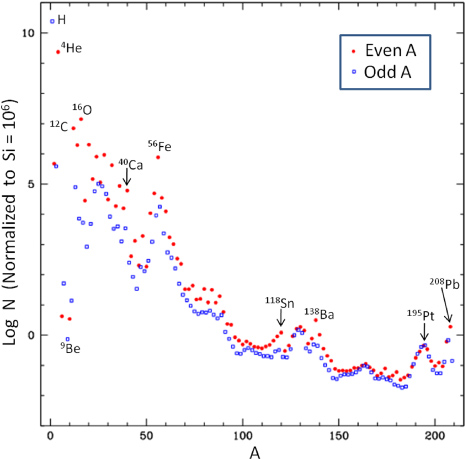
\includegraphics[width=\linewidth]{figures/abundances.jpg}
\caption{The current solar isotopic abundance pattern vs. mass number for even and odd nuclei \cite{Jose2011a}. Abundances are based on both meteoritic samples and observations of the solar photosphere. }
\label{fig: abundances}
\end{figure}

From this point, generations of stellar evolution created nearly all other elements up to iron, with those beyond iron being formed in exotic phenomena, leading to the currently observed elemental abundance distribution, shown in Figure \ref{fig: abundances}. The synthesis of elements heavier than BBN products, commonly referred to as ``metals" by astronomers, began with the formation of the first stars. Cold gas clouds, composed primarily the BBN products of hydrogen and helium (and metals in subsequent stellar generations), coalesce under their mutual gravitational attraction, converting their gravitational potential energy to heat -- increasing their pressure, density, and temperature. Upon passing a critical threshold, typically temperatures $>$1 MK, thermonuclear fusion reactions begin in the core \cite{RyanNortonBook}. This ignition marks the ``birth" of a star, having reached a point where nuclear reactions provide a sufficient heat source to balance energy losses from radiation and stabilize the star's gravitational contraction. 


\subsection{General stellar evolution}

Every star is unique in its intrinsic quantities when forming, such as mass, initial abundance distribution, or subsequent brightness; quantities which prescribe the nuclear reactions that can occur throughout their lifetimes. Despite their differences, correlations emerge in studies of their observational properties, like luminosity, mass distribution, temperature, color, etc. The most evident patterns appeared when classifying stars by luminosity (or magnitude) vs temperature (or color), named the \textit{Hertzsprung-Russel} (HR) diagram \cite{CarrollOstlieBook, IliadisBook, RyanNortonBook}, distilling the most important relationship between stellar properties. An example HR diagram for stars in the solar neighborhood is displayed in Figure \ref{fig: HR_diagram}. Since HR diagrams represent a snapshot of the evolutionary tack of a set of stars, the most densely populated areas of such plots are those in which individual stars necessarily spend most of their lives. Conversely, as there is a lower probability of observing a star in a short-lived phase, sparsely populated areas of HR diagrams detail such phases of stellar burning. 

The vast majority of stars lie on the diagonal band stretching from the upper left (hot, bright stars) to the lower right (cool, faint stars) of the diagram. This feature is called the main sequence. These stars support themselves through core hydrogen burning -- implying that stars spend most of their lives in this long period of quiescent hydrogen burning in the \textit{pp chains} and the CNO cycles, detailed in subsequent sections. Other prominent features of typical HR diagrams are the clusters of stars in the upper quadrants (very bright stars), commonly referred to as the giant branch, the lower left quandrant (hot, faint stars), where the white dwarf stars reside, and the lower right quadrant beyond the main sequence, occupied by brown dwarfs. Each classification corresponds to different nuclear reactions, with stars evolving off the main sequence being characterized by phases of burning of heavier elements, like helium or carbon. 

\begin{figure}
\centering
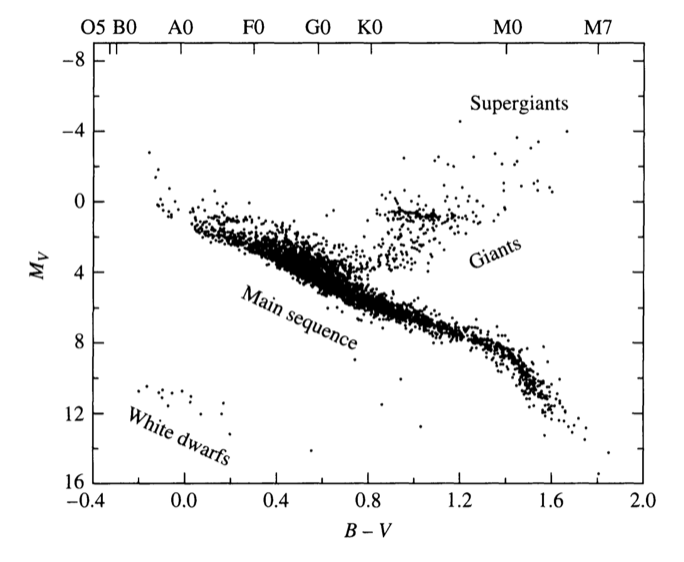
\includegraphics[width=\linewidth]{figures/hrDiagram.png}
\caption{An example of a Herzprung-Russell diagram. The horizontal axis gives the temperature of the star while the vertical shows the stellar luminosities \cite{CarrollOstlieBook}.}
\label{fig: HR_diagram}
\end{figure}

Any single star's evolutionary track will follow different paths depending on its initial mass \cite{IliadisBook, RyanNortonBook}.  For cosmic objects of mass $\lesssim$ 0.08 M$_{\odot}$, where M$_{\odot}$ is the mass of the sun, core temperatures never rise high enough to sustain hydrogen fusion, and thus they evolve directly into brown dwarf stars. In the range of mass 0.08 M$_{\odot} \lesssim$ M $\lesssim$0.4 M$_{\odot}$, stars undergo core hydrogen fusion through the \textit{pp chains}, but do not reach temperatures sufficient to initiate helium burning after exhausting hydrogen in the core. The next mass grouping consists of Sun-like stars, with masses 0.4 M$_{\odot} \lesssim$ M $\lesssim$ 8.0 M$_{\odot}$, which evolve off the main sequence and continue growing and burning (both in the stellar core and shells in their stellar envelope). Such stars achieve temperatures high enough to create final abundance distribution composed of primarily carbon and oxygen in their core. After losing their stellar envelopes, these stars are carbon-oxygen white dwarfs. However, if such a star has a companion of sufficient mass, it will eventually explode in a type Ia supernova. Lastly, are stars of mass M $\gtrsim$ 8.0 M$_{\odot}$, which go through sequences of carbon, neon, oxygen, and silicon burning to produce a dominantly iron-nickel core. At this point, as the stars are more massive than the Chandrasekar limit, the gravitational attraction will exceed the support of electron degeneracy pressure causing a core collapse (type II) supernova. Depending on the star's mass at this stage, it will become either a neutron star or black hole. While not the topic of this thesis, such explosive scenarios are currently an area of intense research as they are the location of many unresolved issues of nuclear astrophysics, including what the National Research Council identified in 2003 as one of the eleven greatest unanswered questions of the century, namely the origin of the elements heavier than iron \cite{Turner2003}, reignited by the 2017 observation of gravitational waves from the neutron star merger GW170817 \cite{Abbott2017}.


\subsection{Hydrogen burning}

The lifetimes of stars along the main sequence vary drastically, from millions of years to trillions of years, depending on the star's properties when forming. Likewise, the dominant type of hydrogen burning that occurs during the main sequence phase is also highly dependent on stellar characteristics like mass and initial composition. Broadly, there are two sets of nuclear processes that comprise the hydrogen burning phases in stellar cores, the \textit{pp chains} and the CNO cycles, with each ultimately functions in a similar way, to convert four hydrogen nuclei to one helium nucleus, releasing $ \sim$26 MeV of energy \cite{RolfsBook}. 

The \textit{pp chains} are the main energy generator in smaller stars with core temperatures below 20 MK \cite{RyanNortonBook}, like the sun. There are three variations of the \textit{pp chains} (denoted ppI, ppII, and ppIII), shown below.

\begin{align*}
\underline{\mathrm{ppI}} & & \underline{\mathrm{ppII}} & &\underline{\mathrm{ppIII}}  & \\
p\left(p, e^{+} \nu \right) d & & p\left(p, e^{+} \nu \right) d & & p\left(p, e^{+} \nu \right) d \\
d\left(p, \gamma \right) \ce{^{3}He} & & d\left(p, \gamma \right) \ce{^{3}He} & & d\left(p, \gamma \right) \ce{^{3}He} \\ 
\ce{^{3}He} \left( \ce{^{3}He}, 2p \right) \ce{^{4}He} & & \ce{^{3}He} \left( \ce{^{4}He}, \gamma \right) \ce{^{7}Be} &  &  \ce{^{3}He} \left( \ce{^{4}He}, \gamma \right) \ce{^{7}Be}  \\
& & \ce{^{7}Be}  \left( e^{-}, \nu \right) \ce{^{7}Li} & & \ce{^{7}Be} \left( p, \gamma \right) \ce{^{8}B} \\
& & \ce{^{7}Li} \left( p, \alpha \right) \ce{^{4}He} & & \ce{^{8}B} \left( e^{+} \nu \right) \ce{^{8}Be} \\
& & & & \ce{^{8}Be} \left( \alpha \right) \ce{^{4}He} 
\end{align*}

Between the three branches there are clear similarities and differences. The energy released between each of ppI, ppII, and ppIII are 26.20 MeV, 25.66 MeV, and 19.75 MeV, respectively, with the difference coming from the amount of energy carried away by the electrons, positrons, and neutrinos \cite{IliadisBook}. Of these chains, ppI is the most prominent, occurring $\sim$ 85 \% of the time, where the remainder branches off as a $\ce{^{3}He}$ nucleus will fuse with a $\ce{^{4}He}$ nucleus, resulting in the ppII or ppIII chain, occurring $\sim$ 14.99 \% and $\sim$ 0.1 \% of the time, respectively \cite{RyanNortonBook}. Regardless of the branching for the \textit{pp chains}, each starts with the $p\left(p, e^{+} \nu \right) d$ reaction. This reaction is governed purely by the weak interaction, and thus is about 20 orders of magnitude slower than those proceeding via the strong interaction \cite{RolfsBook}, like the reactions in the chains that follow. Therefore, energy production, nucleosynthesis, and stellar evolution timescales for stars dominated by the \textit{pp chains} are restricted by the $p\left(p, e^{+} \nu \right) d$ reaction.

However, for more massive stars the CNO cycles are the dominant energy source. Stellar energy generation depends sensitively on the temperature in the star's core, which is closely tied to its mass. For stars of mass M $\gtrsim$ M$_{\odot}$, where cores contain carbon and oxygen seed nuclei and temperatures exceed 20 MK, the CNO cycles' energy production overtakes that of the \textit{pp chains}. Thus, the knowledge of the overall rate of this cycle is important for the study of their evolution. 

The CNO cycles are the collection of four similar energy producing cycles broadly characterized by their synthesis of helium from hydrogen with a carbon catalyst, seeded by earlier generations of stars. There are four CNO cycles, listed below with their relationships shown in Fig. \ref{fig: CNO-cycles}.

\begin{align*}
\underline{\mathrm{CNO1}} & & \underline{\mathrm{CNO2}} & &\underline{\mathrm{CNO3}}  & & \underline{\mathrm{CNO4}} & \\
\ce{^{12}C} \left( p, \gamma \right) \ce{^{13}N} & & \ce{^{14}N} \left( p, \gamma \right) \ce{^{15}O} & & \ce{^{15}N} \left( p, \gamma \right) \ce{^{16}O} & & \ce{^{16}O} \left( p, \gamma \right) \ce{^{17}F}\\
\ce{^{13}N} \left( \beta^{+} \nu \right) \ce{^{13}C} & & \ce{^{15}O} \left( \beta^{+} \nu \right) \ce{^{15}N} & & \ce{^{16}O} \left( p, \gamma \right) \ce{^{17}F} & & \ce{^{17}F} \left( \beta^{+} \nu \right) \ce{^{17}O} \\
\ce{^{13}C} \left( p, \gamma \right) \ce{^{14}N} & & \ce{^{15}N} \left( p, \gamma \right) \ce{^{16}O} & & \ce{^{17}F} \left( \beta^{+} \nu \right) \ce{^{17}O} & & \ce{^{17}O} \left( p, \gamma \right) \ce{^{18}F}\\
\ce{^{14}N} \left( p, \gamma \right) \ce{^{15}O} & & \ce{^{16}O} \left( p, \gamma \right) \ce{^{17}F} & & \ce{^{17}O} \left( p, \gamma \right) \ce{^{18}F} & & \ce{^{18}F} \left( \beta^{+} \nu \right) \ce{^{18}O} \\
\ce{^{15}O} \left( \beta^{+} \nu \right) \ce{^{15}N} & & \ce{^{17}F} \left( \beta^{+} \nu \right) \ce{^{17}O} & & \ce{^{18}F} \left( \beta^{+} \nu \right) \ce{^{18}O} & & \ce{^{18}O} \left( p, \gamma \right) \ce{^{19}F}\\
\ce{^{15}N} \left( p, \alpha \right) \ce{^{12}C} & & \ce{^{17}O} \left( p, \alpha \right) \ce{^{14}N} & & \ce{^{18}O} \left( p, \alpha \right) \ce{^{15}N} & & \ce{^{19}F} \left( p, \alpha \right) \ce{^{16}O}
\end{align*}

\noindent As with the \textit{pp chains}, the net result of each of the CNO cycles is the conversion of four protons into helium, releasing $\sim$ 26 MeV of energy in the process \cite{RyanNortonBook}. Additionally, all of the heavier elements (carbon, nitrogen, oxygen, and fluorine) are only catalysts, with the core still consuming only hydrogen. Since the seed nuclei are not consumed through the process, the overall abundance of these metals in the core is not diminished while their relative abundances evolve with the star. Furthermore, the fact that these nuclei are not destroyed through the reaction chains means that the CNO cycles can occur even if the amount of these heavy elements is relatively small, like in the case of only being seeded by a single prior generation of stars \cite{IliadisBook}. Of the cycles, however, the main CNO1 cycle contributes $\sim$99$\%$ of the CNO energy production \cite{Adelberger1998}, so hereafter CNO1 will be referred to as simply the CNO cycle, while the others will be designated as needed. 

Within the CNO cycle, the $\ce{^{14}N} \left( p, \gamma \right) \ce{^{15}O}$ reaction is the slowest and thus the rate-limiting step of the whole process, ruling the energy production and the overall time spent in this burning phase \cite{Imbriani2004}.

The relative energy production between the \textit{pp chains} and CNO cycles are shown in Fig. \ref{fig: CNO-energy}. It can be seen that the CNO cycle accounts for $< $1 \% of solar energy production \cite{Adelberger1998, Adelberger2011}. However, it produces 1.6 \% of solar neutrinos through the $\beta$-decay of $\ce{^{13}N}$ and $\ce{^{15}O}$ \cite{Bahcall2005a}, which can be used to test assumptions of the Standard Solar Model (SSM), as these rates are one of the largest sources of uncertainty in model predictions \cite{Serenelli2013}. Efforts to measure the neutrino fluxes from the $\beta$-decays of $\ce{^{13}N}$ and $\ce{^{15}O}$ are either ongoing or planned at the Borexino, Super-Kamiokande, and SNO+ laboratories \cite{Jose2011a}.

These laboratories are well known for their contributions in solving the \textsl{solar neutrino problem} \cite{Jose2011a} (and references therein). However, after this solar problem was solved, a new problem arose, named the solar abundance problem \cite{Adelberger2011, Serenelli2009}. The problem is as follows, solar models describe the structure, composition, and evolution of a 1$M_{\odot}$ star from ignition through the sun's current age and are constrained by the plethora of helioseismology data from the Sun. Recent analyses of the Sun's photosphere lead to a reduced metallicity estimate, destroying the agreement between helioseismology and solar models \cite{Asplund2009}. In discussing potential solutions to this problem, it was proposed to use the neutrino fluxes from the $\beta$-decay of CNO isotopes $\ce{^{13}N}$ and $\ce{^{15}N}$ to address this problem, as these quantities depend linearly on their abundance within the solar core \cite{Bahcall2005a, Bahcall2005b}. As a part of the CNO cycles, there are the $\beta^{+}$-decays of and the electron captures on $\ce{^{13}N}, \ce{^{15}O},$ and $\ce{^{17}F}$.  Each of these interactions produces neutrinos but the overall rate of these processes as a part of the CNO cycle in the sun is again limited by the $\ce{^{14}N} \left( p, \gamma \right) \ce{^{15}O}$, which is again the slowest step in the overall cycle. Therefore, a more precise understanding of these neutrino fluxes (like the example given in Fig.\ \ref{fig: neutrinoSpectrum}), requires ever more precise knowledge of the relevant nuclear cross-sections, as the fluxes from CNO neutrinos are one of the largest uncertainties present. 



\begin{figure}
\centering
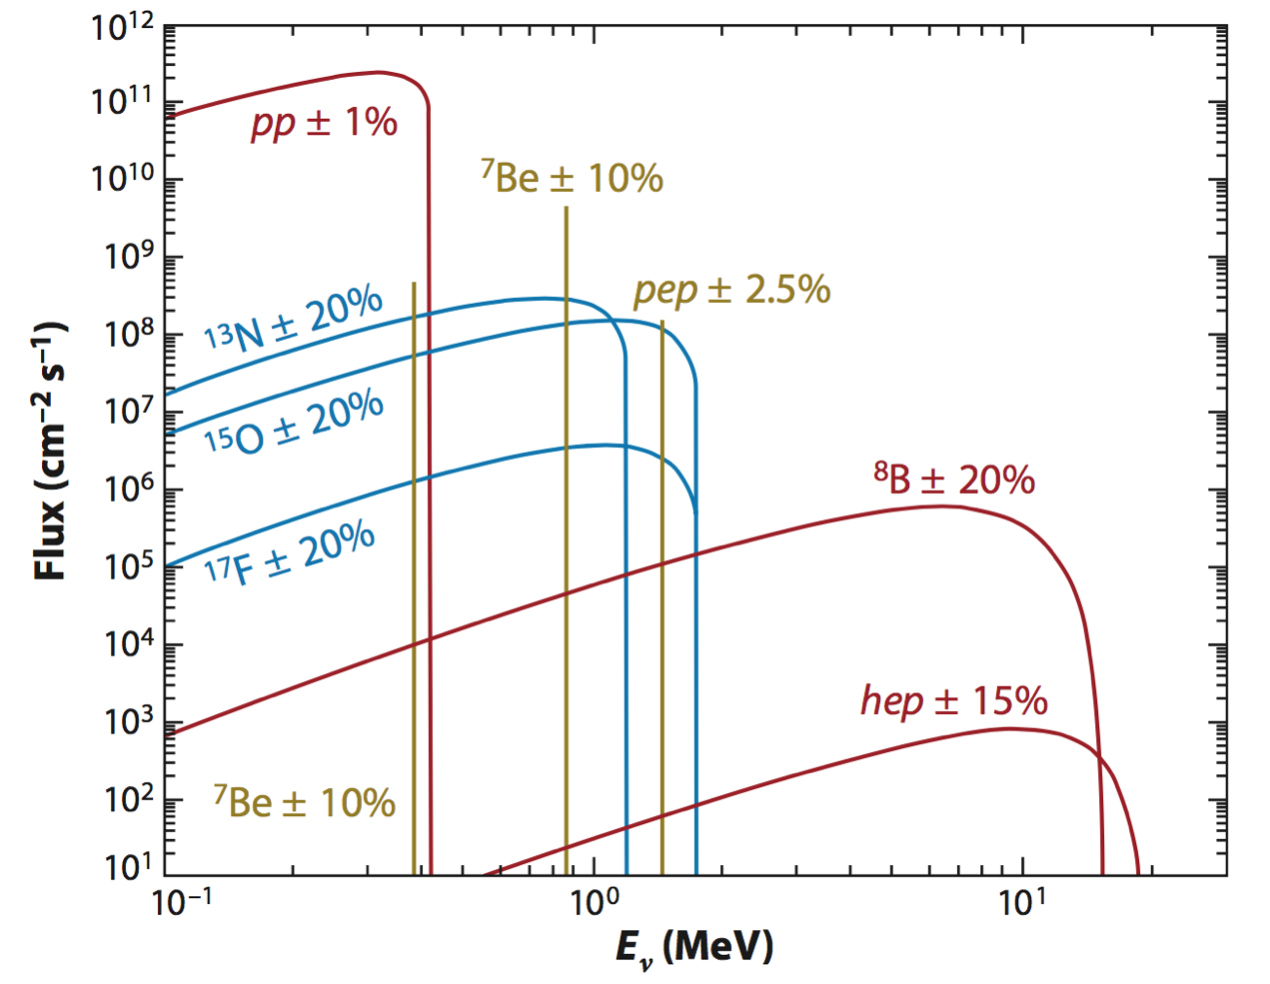
\includegraphics[width=\linewidth]{figures/neutrinoFlux.png}
\caption{Predicted solar neutrino flux spectrum, taken from \cite{Wiescher2010} and produced from data in \cite{Bahcall2004}.   }
\label{fig: neutrinoSpectrum}
\end{figure}



In fact, in 2020, the Borexino collaboration reported the first measurement of the solar CNO neutrino flux \cite{agostini2020direct}. This result can be seen in Fig.\ \ref{fig: borexinoSpectrum}. The contributions to the neutrino flux from different sources are separated and noted. The highlighted region represents the point of best separation between the CNO neutrinos and those coming from other sources. After nearly a decade of measurements, the collaboration was able to constrain the background neutrino rates coming from the beta decays of $^{210}$Bi (intrinsic to the detector) and the proton-electron-proton reaction ($p^{+} + e^{-} + p^{+} \rightarrow ^{2}$H$ + \nu_{e}$) in the \textit{pp chains} \cite{agostini2020sensitivity}. The authors were able to extract the CNO contribution with a multivariate fit, for the first time confirming the presence of solar CNO neutrinos (and at a $5 \sigma $ level). The Borexino collaboration reported a flux higher than those inferred from other measurements of the relevant cross-sections. Following this result, it is critical to understand the nuclear physics inputs, particularly those coming from the $\beta$ decay of $^{15}$O, in order to resolve discrepancies between solar models and helioseismology.


\begin{figure}
\centering
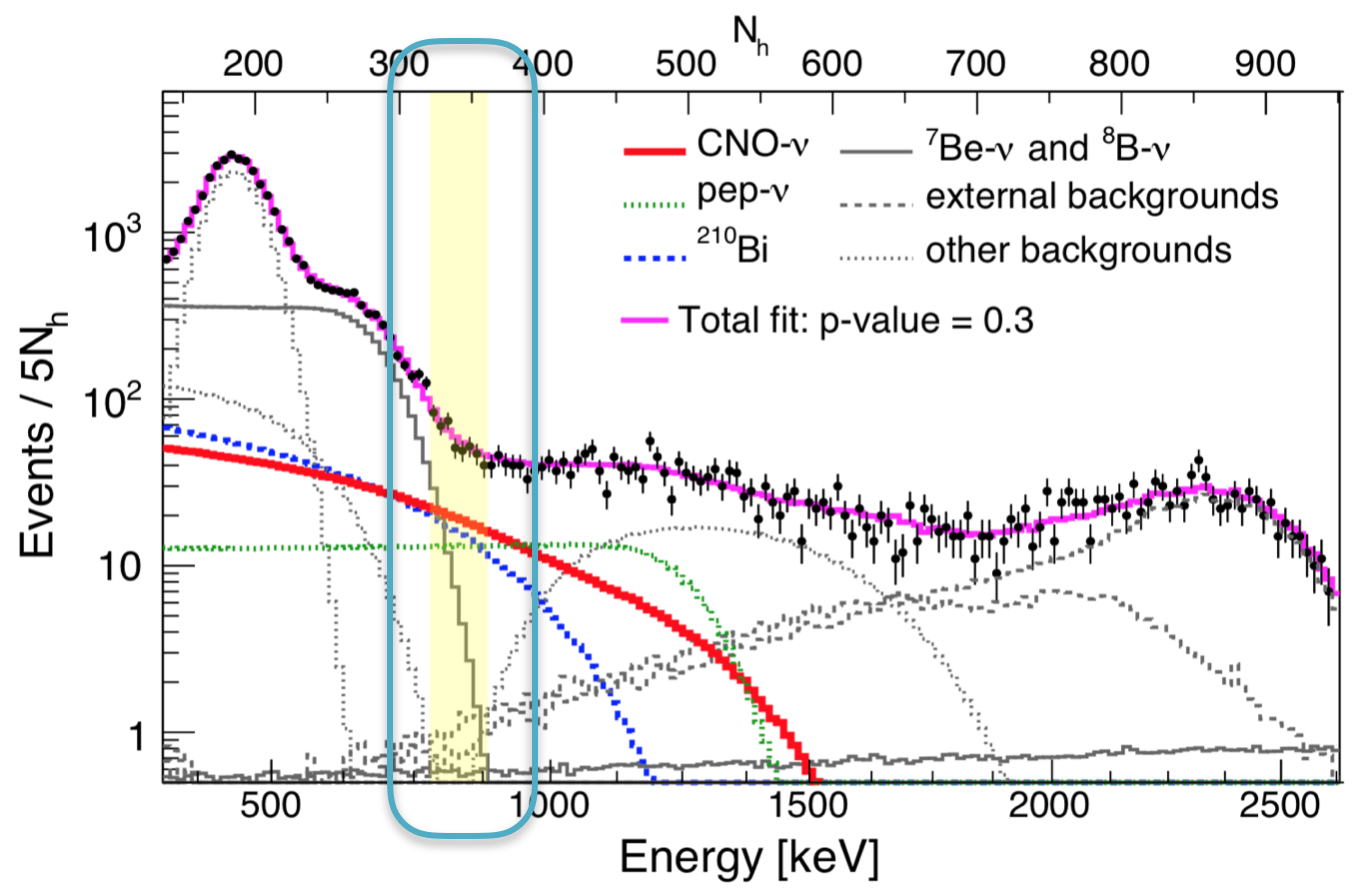
\includegraphics[width=\linewidth]{figures/borexino_result.png}
\caption{Energy distribution of events measured in the Borexino detector (black), and the spectral fit to the data (magenta), taken from \cite{agostini2020direct}. The contributions from different sources are are separated and noted. The highlighted region (with the additional box for emphasis) represents the region with the highest signal-to-background ratio for the CNO neutrinos. It is by measuring this energy range precisely that the authors determined the CNO contribution to the solar neutrino flux. Following this measurement, it is critical to understand the nuclear physics inputs, particularly those coming from the $\beta$-decay of $^{15}$O, in order to resolve discrepancies between solar models and helioseismology.   }
\label{fig: borexinoSpectrum}
\end{figure}


\begin{figure}
\thisfloatpagestyle{plain}
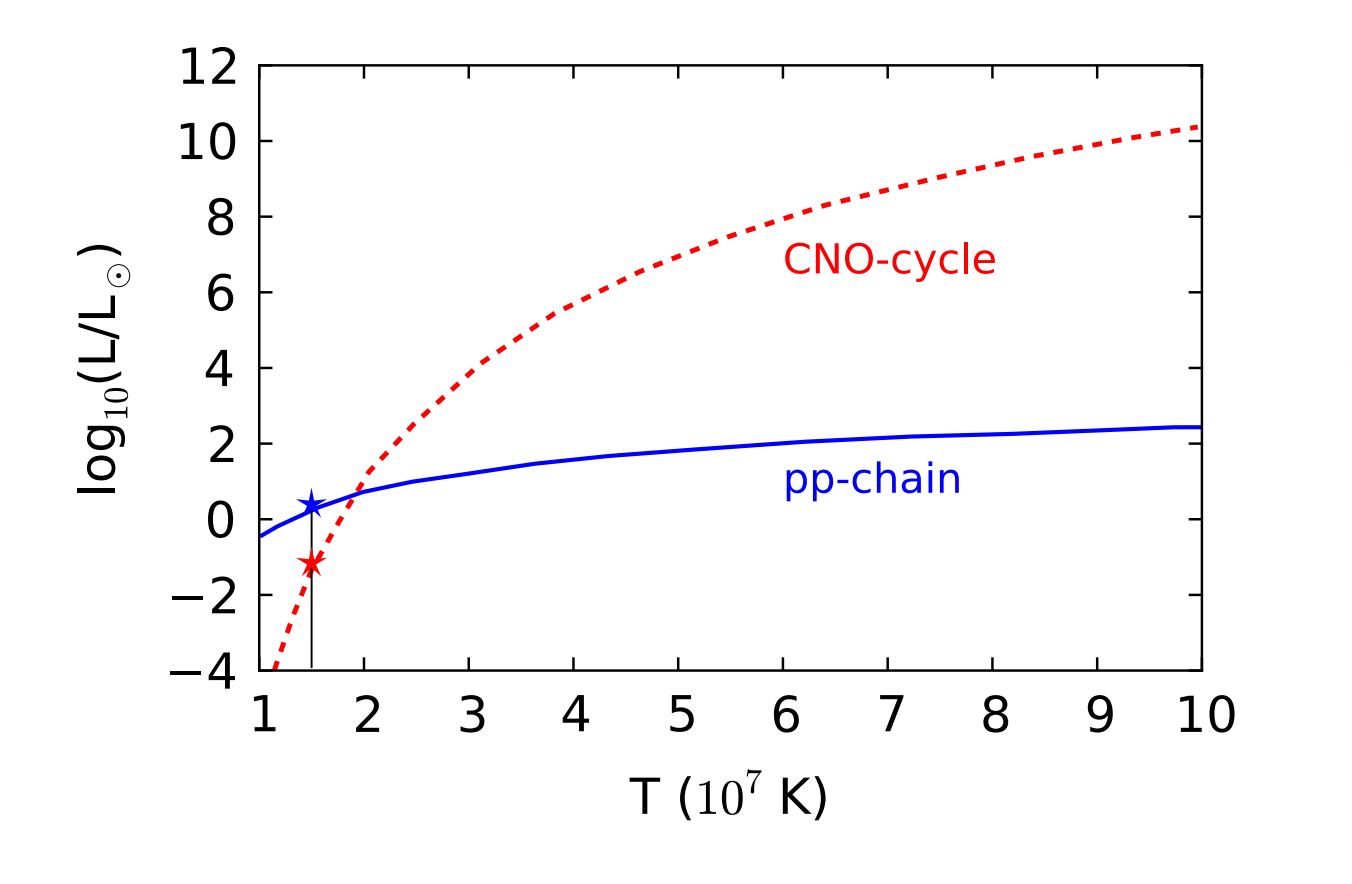
\includegraphics[width=\linewidth]{figures/energyProduction.png}
\caption{Energy dependence of the \textit{pp chains} and the CNO cycles as a function of stellar temperature assuming a solar abundance distribution of CNO elements \cite{Bertulani2016}. The sun's temperature is marked with the star in the figure. This shows that for lower mass stars like the sun the \textit{pp chains} are the dominant mode of energy production in main sequence burning. However, for hotter, more massive stars, the CNO cycle quickly dominates. }
\label{fig: CNO-energy}
\end{figure}



Due to the importance of the $\ce{^{14}N} \left( p, \gamma \right) \ce{^{15}O}$ reaction, it is the focus of this work. Presented first, in Sec. \ref{sec: thermonuclear reaction rates} and Sec. \ref{sec: reactions} are an overview of nuclear reactions and reaction theory relevant for nuclear astrophysics. An extension of these theories using the $R$-matrix formalism will be presented in Sec. \ref{sec: r-matrix}. The current state of knowledge surrounding the reaction, its uncertainties, and previous measurements are discussed in Sec. \ref{sec: 14N(p,g)}. Finally, an outline of the remainder of this work will be presented in Sec. \ref{sec: thesis outline}.


\begin{figure}
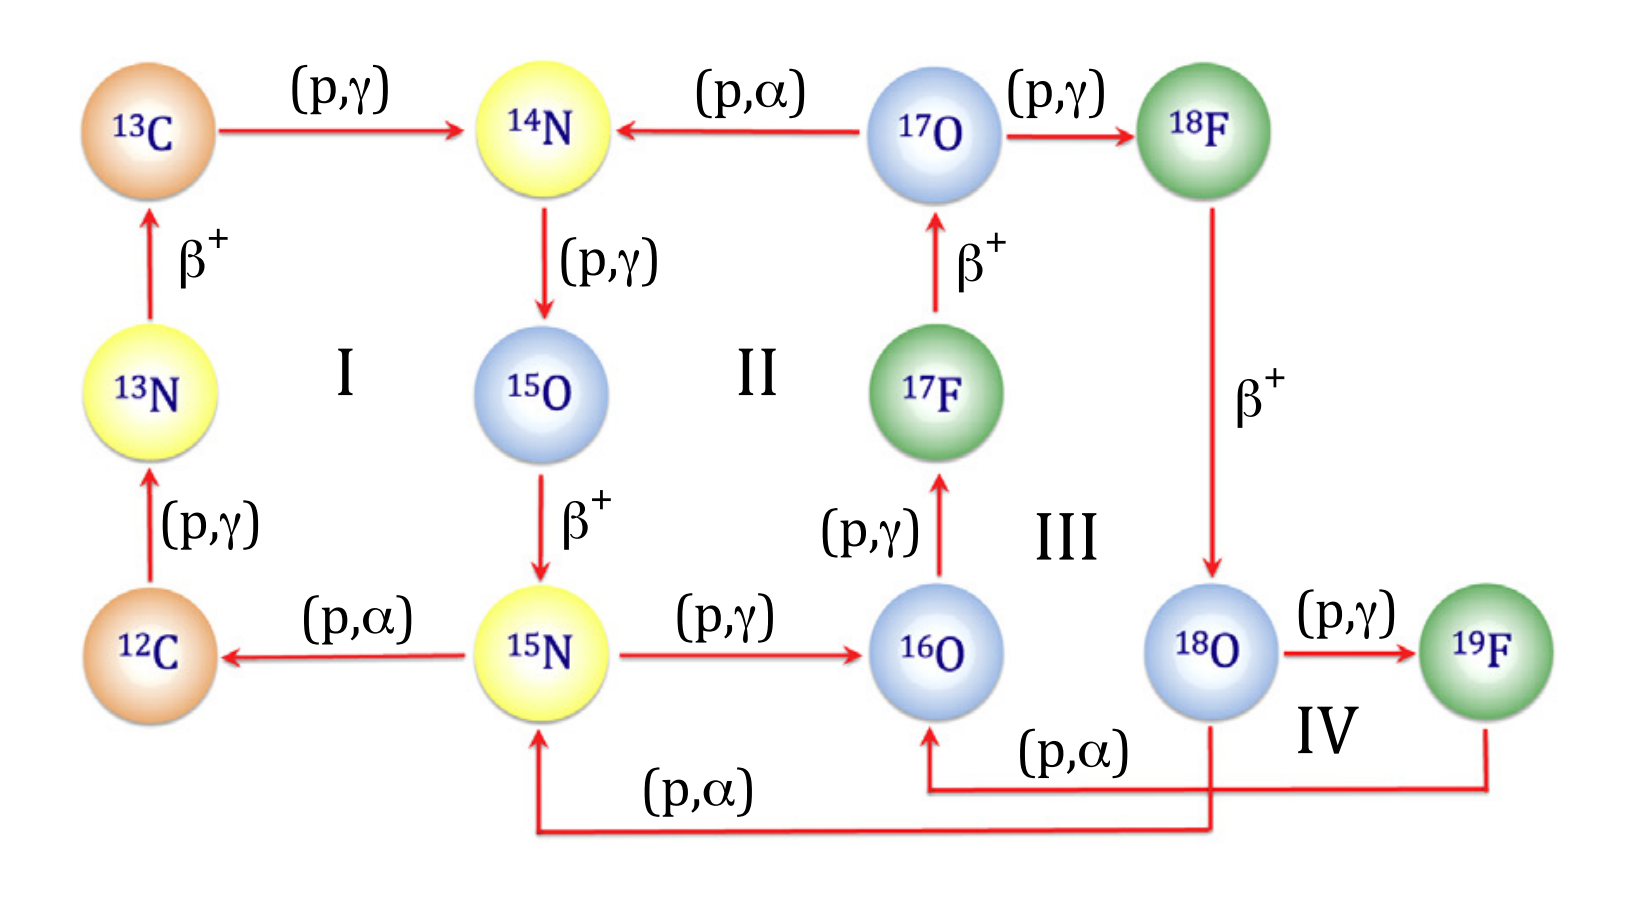
\includegraphics[width=\linewidth]{figures/cnoCycles.png}
\caption{A depiction of the CNO cycles for hydrogen burning in stars \cite{Bertulani2016}. Cycles II, III, and IV only contribute meaningfully at very high temperatures or explosive burning scenarios. }
\label{fig: CNO-cycles}
\end{figure}




\section{Thermonuclear reaction rates}
\label{sec: thermonuclear reaction rates}

Stars are fueled by the energy released during nuclear reactions. A nuclear reaction can be written as 

\begin{equation}
a + A \rightarrow b + B + Q \hspace{0.5in} \text{or} \hspace{0.5in} A(a,b)B^{*}
\end{equation}

\noindent where $a$ denotes the projectile, $A$ the target nucleus, $b$ the ejectile, $B$ the reaction product, and $Q$ the energy released (or absorbed) during the reaction, typically present as kinetic energy distributed among the reaction products. For this reaction to occur, the initial nuclei must have enough energy to overcome the Coulomb repulsion created by their constituent protons. The probability of their interaction, called their cross section ($\sigma$), is therefore energy dependent. As stars are powered by thousands of such reactions at a variety of energies, the understanding of nuclear cross-sections are crucial components to the subsequent understanding of stellar evolution and nucleosynthesis. 

Consider a stellar environment filled with two types of nuclei with number densities (nuclei / cm$^{3}$) $N_{1}$ and $N_{2}$, respectively, and relative velocity $v$. The rate of reaction for these two species per unit volume would then be proportional to the probability that a given pair of particles would react multiplied by the number of pairs that interact per unit time. Mathematically, the reaction rate $R_{12}$ would therefore be

\begin{equation}
R_{12} = \dfrac{N_{1} N_{2}}{1+\delta_{12}} v \sigma (v)
\label{eqn: rr general}
\end{equation}

\noindent with $\delta_{12}$ to prevent overcounting if the particles are identical. In stellar environments, the relative velocity between the two particles can take a range of values related to the temperature, $T$. The probability distribution of the potential relative velocities, $P(v)$, is described by the Maxwell-Boltzmann distribution \cite{RyanNortonBook}: 

\begin{equation}
P(v) = 4 \pi v^{2} \left( \dfrac{\mu}{2\pi k T} \right)^{3/2} \exp \left( - \dfrac{\mu v^{2}}{2 k T} \right)
\label{eqn: mb distribution}
\end{equation}

\noindent where $k$ is the Boltzmann constant, relating the kinetic energy of a particle to the temperature of its environment, and $\mu = m_{1}m_{2}/(m_{1}+m_{2})$ is the reduced mass of the two nuclei. Explicitly, the probability that a given pair of nuclei having a relative velocity between $v$ and $v+dv$ is $P(v)dv$ and satisfies the unity expression

\begin{equation}
\int_{0}^{\infty} P(v) dv = 1.
\end{equation}

Therefore, the reaction rate per particle pair $\langle \sigma v \rangle$ with relative velocity $v$ is the average value of $v$ multiplied with $\sigma(v)$ for a given temperature,

\begin{equation}
\langle \sigma v \rangle = \int_{0}^{\infty} v P(v) \sigma(v) dv.
\label{eqn: rr condensed}
\end{equation}

\noindent Using a few useful substitutions, this formulation allows us to rewrite Equation \ref{eqn: rr general}, the general reaction rate, as a function of energy instead of velocity. To do this, recall that the kinetic energy is $E = \dfrac{1}{2} \mu v^{2}$ and its derivative is $dE / dv = \mu v$. By explicitly writing the Maxwell-Boltzmann distribution into and replacing the appropriate terms in Equation \ref{eqn: rr condensed} leads to 

\begin{equation}
\langle \sigma v \rangle = \left( \frac{8}{\pi \mu} \right) ^{1/2} \left( \frac{1}{kT} \right) ^{3/2} \int_{0}^{\infty} \sigma (E) E \exp \left(-\dfrac{E}{kT} \right) dE.
\label{eqn: rr full}
\end{equation}

\noindent It is important to note that the only unknown in the entirety of the reaction rate is the expression of the nuclear cross section as a function of energy, $\sigma(E)$.  Therefore, to understand the reaction rates for stellar environments, $\sigma(E)$ needs to be determined. 

While the cross section, $\sigma(E)$, is an expression of the probability of two nuclei reacting when brought together at a specific energy, $E$, it is analogous to the classical, cross-sectional area of the nucleus, so it is expressed in units of area (specifically barns, where 1 b = $10^{-24}$cm$^{2}$). An insightful description is to think of the cross section coming from throwing two balls at each other with random perturbations off of a common axis, classically. If either ball's size changes (cross-sectional area), the chances of hitting will also change in a manner that is directly proportional to the alteration of the respective sizes of the balls since the total cross-sectional area is $\sigma = \pi (R_{1} + R_{2})^{2}$. For our quantum mechanical nuclei, the nuclear size needs to be replaced with the deBroglie wavelength, resulting in $\sigma = \pi \lambdabar$. Translating this into another formulation that is more familiar, the cross section is the number of reactions occurring divided by the number of potential reactions, given as

\begin{equation}
\sigma = \dfrac{N_{R}}{(N_{i} N_{t})/A},
\end{equation}

\noindent where $N_{R}$ is the number of reactions that take place per unit time, $N_{i}$ is the number of incident nuclei per unit time, $N_{t}$ is the number of target nuclei within the area of incidence, $A$. 

In astrophysical environments, nuclei typically do not have enough energy to overcome the Coulomb repulsion, which is given as $V_{C} = Z_{0}Z_{1}e^{2}/R_{n}$ with $R_{n}$ is the nuclear radius, provided by the protons within the nucleus and combine with the attractive nuclear strong force. A diagram of the combined nuclear and Coulomb potentials is given in Fig. \ref{fig: potentials}. The repulsive Coulomb interaction causes the cross section to drop quickly at low center-of-mass energies \cite{IliadisBook}. Thus, for such reactions to occur, nuclei must actually tunnel through the Coulomb barrier. 

\begin{figure}
\thisfloatpagestyle{plain}
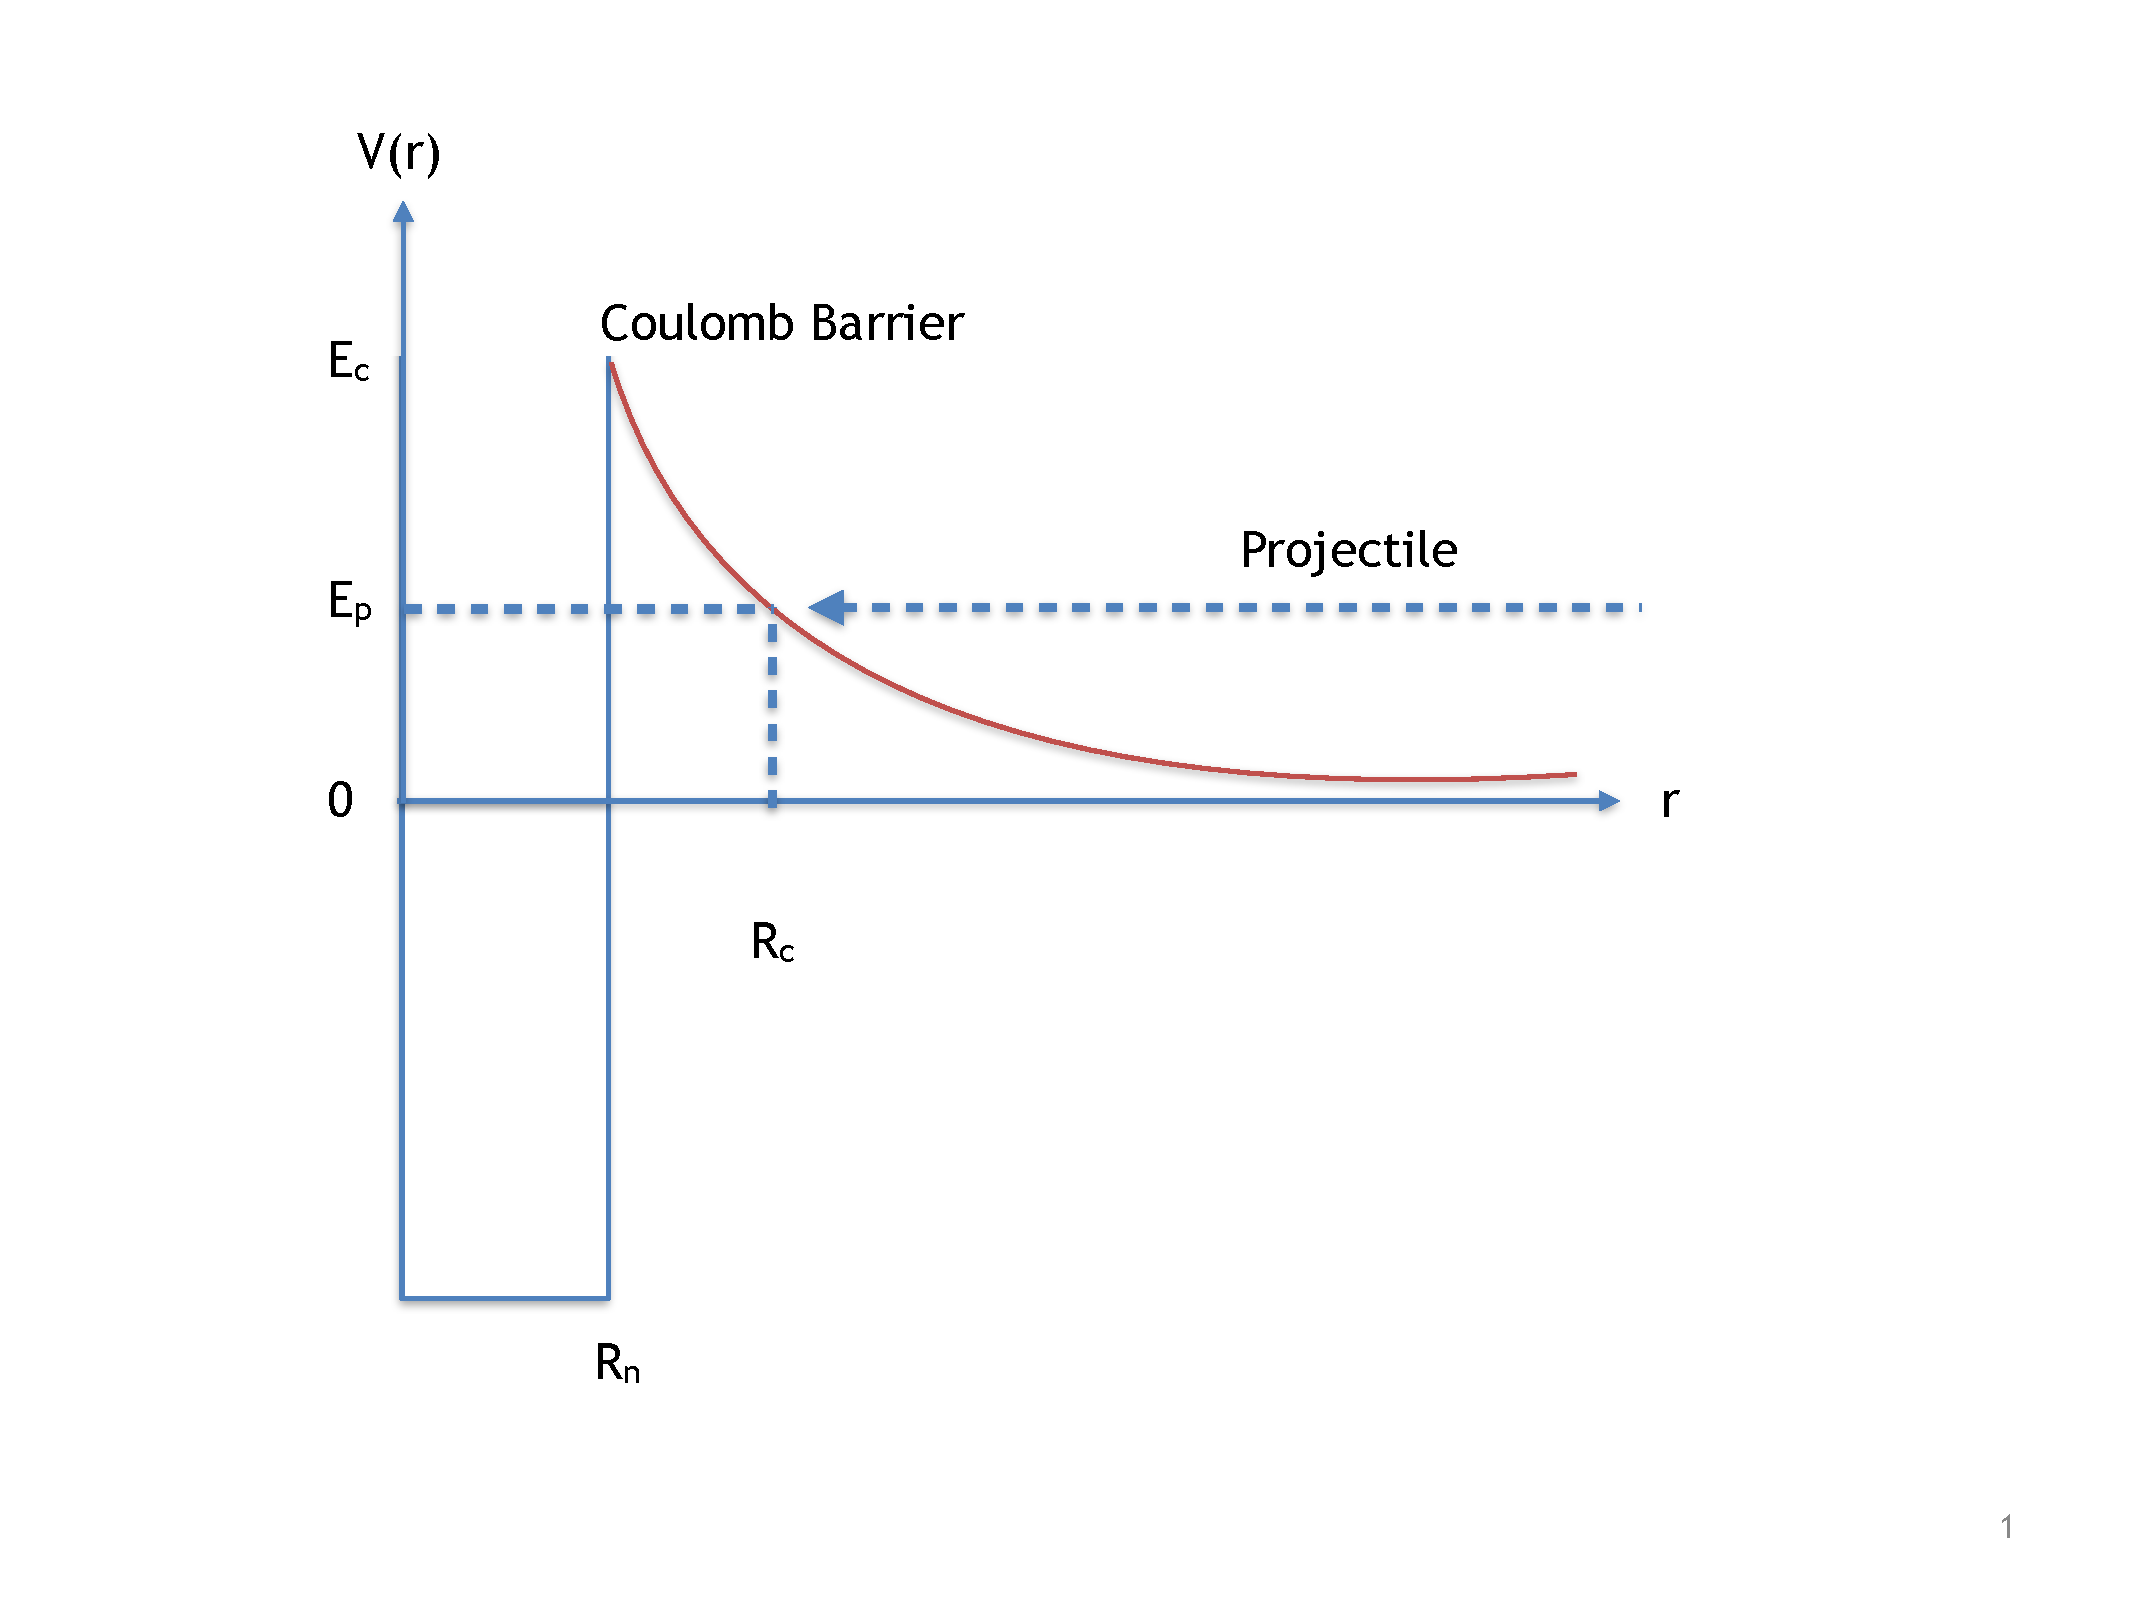
\includegraphics[width=\linewidth]{figures/potentials.pdf}
\caption{Schematic plot of the combined attractive nuclear and repulsive Coulomb potentials where $R_{n}$ is the nuclear radius, $R_{c}$ is the classical turning point due to Coulomb repulsion, $E_{c}$ is the height of the Coulomb barrier, and $E_{p}$ is the projectile's energy. Because this is a quantum system, the projectile has a chance to tunnel through the Coulomb barrier and make it into the attractive nuclear potential when it has energy $E_{p} < E_{c}$. }
\label{fig: potentials}
\end{figure}

The Coulomb penetrability, $P$, can be approximated as the leading term of the $s$-wave ($\ell$ = 0) barrier transmission coefficient:

\begin{equation}
P = \exp(-2\pi\eta),
\end{equation}

\noindent where $\eta$ is the Sommerfeld parameter,

\begin{equation}
\eta = \dfrac{Z_{1}Z_{2}e^{2}}{4 \pi \epsilon_{0} \hbar v} = \alpha Z_{1} Z_{2} \sqrt{\dfrac{\mu c^{2}}{2E_{cm}}},
\end{equation}

\noindent where $Z_{i}$ is the respective proton number of each nucleus, $v$ is the incident center-of-mass velocity, $\alpha \approx 1/137$ is the fine-structure constant, $\mu$ is the reduced mass of the system, and $E_{cm}$ is the center of mass energy of the interacting nuclei. Numerically, it is convenient to evaluate the quantity $2\pi \eta$, known as the Gamow factor, as

\begin{equation}
2\pi \eta = 0.989534 Z_{1} Z_{2} \left( \dfrac{\mu}{E_{cm}} \right)^{1/2}, 
\label{eqn: gamow factor}
\end{equation}

\noindent where $E_{cm}$ is expressed in units of MeV and $\mu$ in atomic mass units (amu or simply, u). 

By factoring the Coulomb penetrability out of the cross section, we can separate the contributions from the Coulomb barrier to isolate the nuclear physics in the astrophysical $S$-factor, $S(E)$, 

\begin{equation}
\sigma(E) = \dfrac{1}{E} S(E) e^{-2\pi \eta}.
\label{eqn: s-factor definition}
\end{equation}

\noindent The astrophysical $S$-factor is more slowly varying with energy over the Gamow window (in the absence of resonances) when compared to the nuclear cross section. Fig. \ref{fig: energy dependence} provides a comparison of the energy dependence of both the cross section and $S$-factor, where you can see that the cross section drops by orders of magnitude in an energy regime where the $S$-factor is relatively constant. This implies that the Coulomb effects can obscure important nuclear physics effects. Additionally, as the $S$-factor is slowly varying, extrapolations of it's behavior towards zero energy from higher energy data are significantly more reliable than those made from cross section data. 

\begin{figure}
\thisfloatpagestyle{plain}
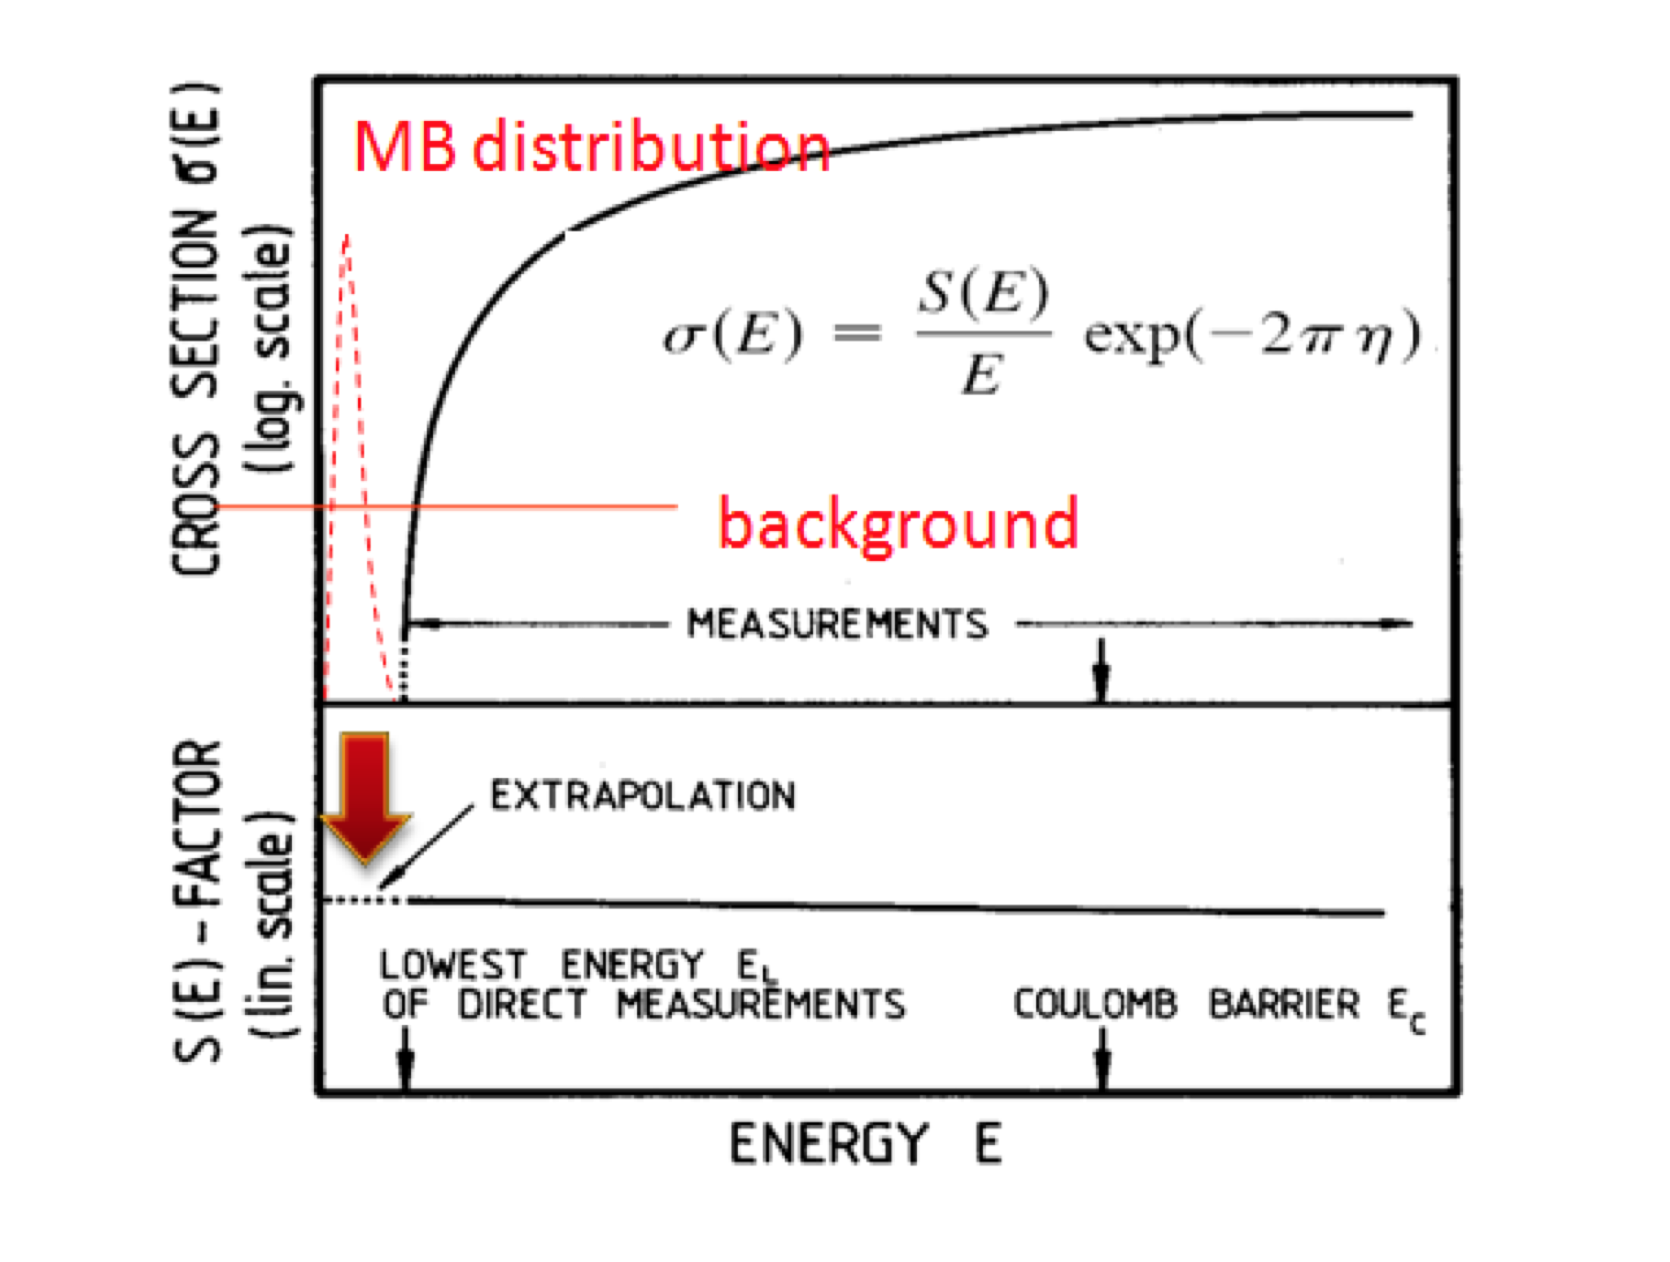
\includegraphics[width=\linewidth]{figures/crossSectionDependence.png}
\caption{The energy dependence of the nuclear cross section and astrophysical S-factor \cite{RolfsBook}. The cross section drops dramatically due to Coulomb repulsion as the incident energy drops, however the $S$-factor, by removing the Coulomb penetrability varies slowly towards the Gamow window (barring the absence of nuclear resonances). }
\label{fig: energy dependence}
\end{figure}

Now, after defining the $S$-factor, the reaction rate can be written finally as 

\begin{equation}
\langle \sigma v \rangle = \left( \frac{8}{\pi \mu} \right) ^{1/2} \left( \frac{1}{kT} \right) ^{3/2} \int_{0}^{\infty} S (E) \exp \left(-\dfrac{E}{kT} - \dfrac{b}{E^{1/2}}\right) dE.
\label{eqn: Rrate with sfac}
\end{equation}

\noindent where $b$ has units of (MeV)$^{1/2}$ and is given as

\begin{equation}
b = 0.989534 Z_{1} Z_{2} \mu^{1/2}. 
\end{equation}

\noindent Recall that one of the most useful features of $S(E)$ is that it is typically smoothly varying with respect to energy, meaning that the reaction rate in total is dependent primarily on the exponential term inside the integrand of Eq. \ref{eqn: Rrate with sfac}. The two components of this term arise from the Coulomb penetrability and the Maxwell-Boltzmann velocity distribution described in Eq. \ref{eqn: mb distribution}. The convolution of these two quantities can be used to estimate the energy range where the reaction rate should be maximized for given stellar temperatures \cite{IliadisBook}. 

The Coulomb penetrability and Maxwell-Boltzmann velocity distribution have opposite behaviors in energy regimes with the penetrability dropping to zero at low energies while the probability distribution for the velocities is maximized at low energies and vice-versa at high energies. The product of the terms is therefore negligible for nearly all energies. However, for a small set of energies this product, and therefore the reaction rate, maximizes. This behavior, as well as their product, commonly called the Gamow Peak, is presented in Fig. \ref{fig: Gamow Peak}. 

The Gamow peak's maximum can be obtained with basic calculus on the exponential term in Eq. \ref{eqn: Rrate with sfac} by setting the derivative with respect to energy equal to zero and solving for the energy value. This results in the maximum energy of the reaction rate being 

\begin{figure}
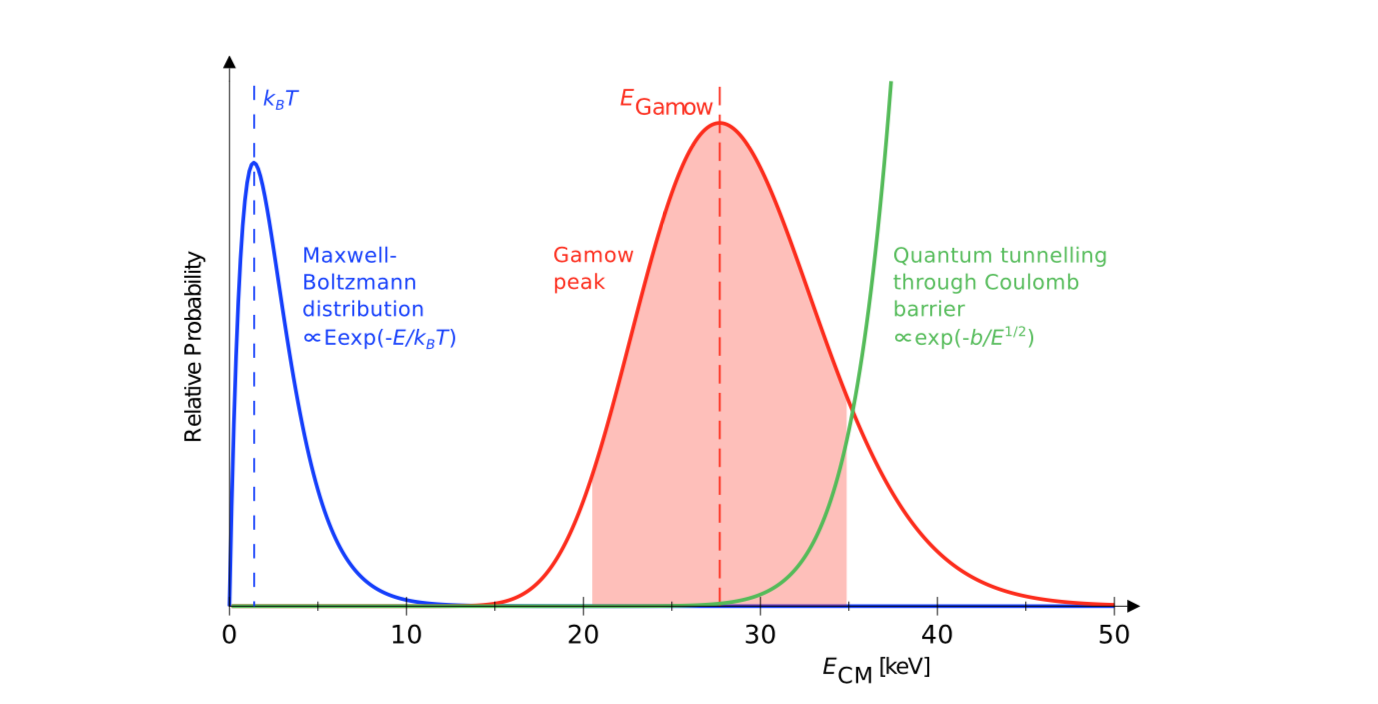
\includegraphics[width=\linewidth]{figures/gamowWindow.png}
\caption{The two dominant terms of the reaction rate calculation and their convolution (Gamow peak) for the $\ce{^{14}N}(p,\gamma)\ce{^{15}O}$ reaction at $T = 0.016$ GK \cite{Bemmerer2004}. The y-axis is given in arbitrary units.}
\label{fig: Gamow Peak}
\end{figure}

\begin{equation}
E_{0} = \left( \dfrac{b k T}{2}  \right)^{2/3}. 
\label{eqn: GamowPeak}
\end{equation}

\noindent For a given stellar temperature, $T$, the average effective energy at which the reaction occurs is $E_{0}$. Additionally, this also allows for an approximation of the range of energies over which the reaction primarily occurs, provided that the $S$-factor is smoothly varying (which is not true if resonances are present, which will be discussed in the next section). This range of energies is known as the Gamow Window, $\Delta$:

\begin{equation}
\Delta = \dfrac{4}{\sqrt{3}} \sqrt{E_{0} k T}.
\label{eqn: Gamow window width}
\end{equation}

\noindent The Gamow window identifies the range of energies as a function of temperature over which experimental data should be taken to provide a complete understanding of stellar processes and the interplay of the Maxwell-Boltzmann velocity distribution with the Coulomb penetrability to create the Gamow window is presented in Fig. \ref{fig: Gamow Peak}. As an example, the $\ce{^{14}N} \left( p, \gamma \right) \ce{^{15}O}$ reaction in the sun has a Gamow peak energy at $E_{0} = 26.6$ keV and $\Delta = 13.6$ keV, meaning that measuring the cross section in the energy range of 19.8 - 33.4 keV is crucial in the understanding of this reaction. 

Unfortunately, though, measuring at energies this low is not feasible, experimentally. This is because at these energies the signal-to-noise ratio of observables drops dramatically and the signals of interest are obscured within background noise. To provide accurate measurements of such situations, experiments must necessarily then occur in the timescale of years to measure a single datum. This is simply unfeasible, practically, and our understanding must rely on extrapolations from higher-energy data. As the $\ce{^{14}N} \left( p, \gamma \right) \ce{^{15}O}$ reaction is not alone in having a Gamow window at such low energies, extrapolation techniques must be employed to describe the cross section and $S$-factor for nearly all astrophysically important reactions at the Gamow window. This, then, in a nutshell highlights the primary goal of experimental nuclear astrophysics: to a) directly measure relevant cross-sections down to astrophysical energies when possible, or b) measure as low in energy as possible to provide the best constraint for theoretical extrapolations to Gamow energies.



\section{Nuclear reactions}
\label{sec: reactions}

For the $\ce{^{14}N} \left( p, \gamma \right) \ce{^{15}O}$ reaction, both resonant and direct capture contributions are important. Resonant reactions are those in which an incoming particle combines with a target to form an excited state in a compound nucleus and then subsequently decay as part of a two-step process. Alternatively, direct capture reactions are those in which the particle pair proceeds directly to a final, bound nuclear state in one step. An energy level diagram of the $\ce{^{14}N} \left( p, \gamma \right) \ce{^{15}O}$ reaction is shown in Fig. \ref{fig: level diagram}.

\begin{figure}
\thisfloatpagestyle{plain}
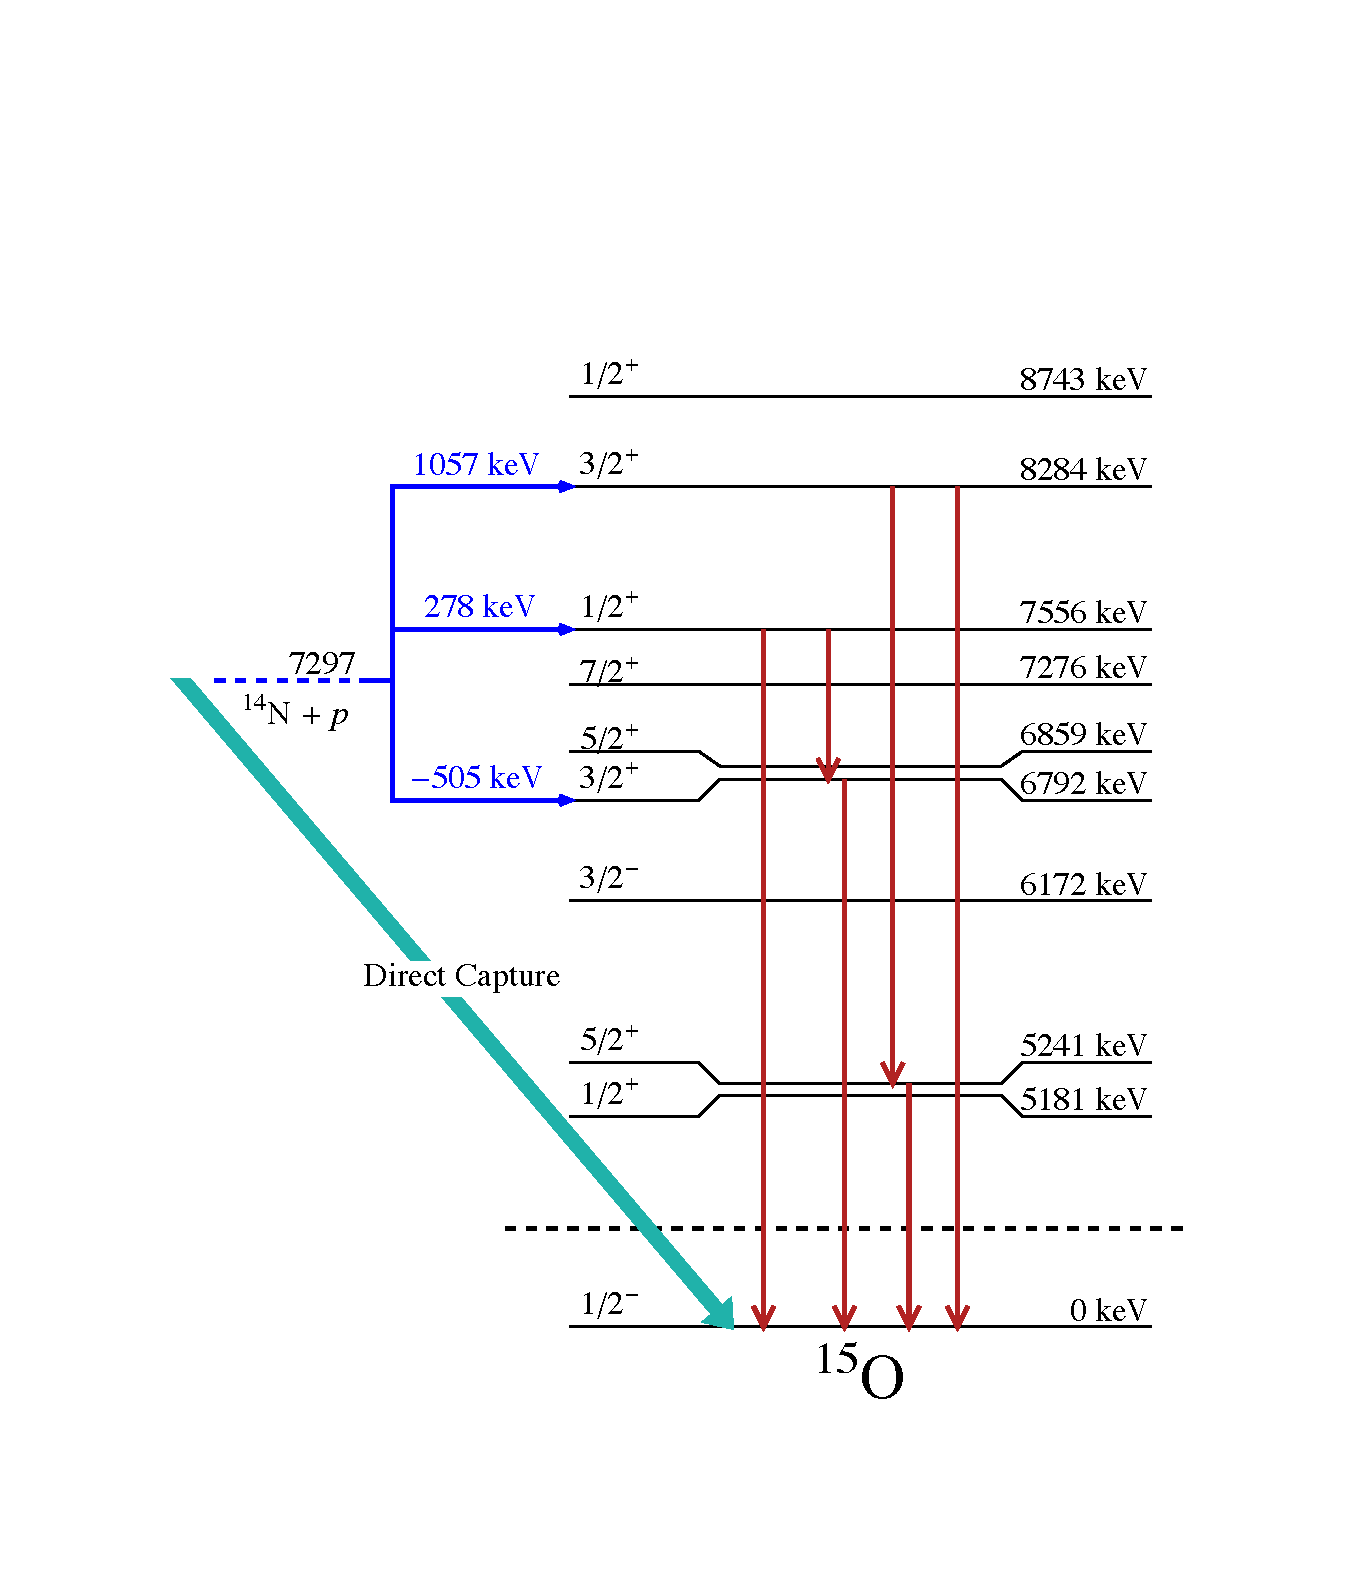
\includegraphics[width=\linewidth]{figures/levelsO15.pdf}
\caption{An energy level diagram of the $\ce{^{14}N} \left( p, \gamma \right) \ce{^{15}O}$ reaction. This shows the pathways of decay to the ground state of the $\ce{^{15}O}$ nucleus. The paths shown in red indicate a resonance reaction, with the formation of the compound nucleus in an excited state, while the path in green shows a direct capture process, proceeding immediately to the final state (ground in this example) from any energy above the proton threshold.}
\label{fig: level diagram}
\end{figure}




\subsection{Direct capture reactions}

The other side of the proverbial coin from resonant reactions is direct capture, or nonresonant reactions. Such cases are defined as those in which the cross section and $S$-factor vary smoothly with energy, being the result of a one-step, electromagnetic process where the capture proceeds from the initial state of two incident particles to the final, bound state of the system. This is process is also highlighted as a part of Fig. \ref{fig: level diagram}. 

With nonresonant reactions, the $S$-factor varies smoothly with energy. This means that the earlier characterization  of the $S$-factor, reaction rate, and Gamow energy/window parameters in Equations \ref{eqn: rr full} - 
\ref{eqn: Gamow window width} are applicable for the case of direct reactions. In extrapolating experimental data to stellar energy ranges, it is often useful to express an effective $S$-factor, $S_{\text{eff}}$ from the Taylor expansion of the component functions \cite{IliadisBook},

\begin{equation}
S_{\text{eff}} = S(0) \left( 1 + \dfrac{5 k T}{36 E_{0}}   \right) + S'(0) E_{0} \left( 1 + \dfrac{35 k T}{36 E_{0}}   \right)  + \dfrac{1}{2} S''(0) E_{0}^{2} \left( 1 + \dfrac{89 k T}{36 E_{0}}   \right),
\label{eqn: Seff}
\end{equation}

\noindent where $E_{0}$ is the Gamow peak energy from Equation \ref{eqn: GamowPeak}. Armed with this expansion, the $S$-factor can be successfully extrapolated to low, stellar energies in cases where the $S$-factor varies slowly with energy. This means that for nonresonant reactions, $S(E)$ can be approximated by its zero-energy value, $S(0)$, and only small corrections given by its first and second derivatives, $S'(0)$ and $S''(0)$, respectively. 




\subsection{Resonant reactions}

The presence of a resonance enhances the cross section at its specific center-of-mass energy and means that the $S$-factor no longer varies smoothly with respect to energy. The specific increase is highly dependent on the situation since, as a two-step process, it depends on the probability of both forming the compound nucleus and decaying via a specific pathway, also shown in Fig. \ref{fig: level diagram}. To understand this mathematically, consider an isolated, narrow resonance at energy $E_{R}$; the reaction cross section under the influence of such a resonance is described by the Breit-Wigner formula:

\begin{equation}
\sigma_{BW}(E) = \pi \lambdabar^{2} \frac{2J_R+1}{(2J_1+1)(2J_2+1)}\frac{\Gamma_\mathrm{in}\Gamma_\mathrm{out}}{(E-E_{R})^2+\Gamma_{T}^2/4}
\label{eqn: BreitWigner}
\end{equation}

where $\lambdabar$ is the deBroglie wavelength corresponding to the incident momentum, $p=\hbar/\lambdabar$, $J_1$ and $J_2$ are the spins of the target and projectile, $J_R$ is the spin of the resonance in the compound nucleus, $\Gamma_\mathrm{in}$ and $\Gamma_\mathrm{out}$ are the entrance and exit reaction channel widths (essentially the probability for a particular part of the process to occur), and $\Gamma_T$ is the total width ($\Gamma_t = \Gamma_1 + \Gamma_2 + ... \Gamma_n$). The total width is related to the mean lifetime, $\tau$, of the excited state through the Heisenberg Uncertainty Principle by 

\begin{equation}
\tau \Gamma_{T} = \hbar.
\label{eqn: width to lifetime}
\end{equation}

For most nuclear states, the widths can be determined experimentally, allowing for the understanding of the total width, $\Gamma_{T}$. However, due to many of the earlier described constraints, this is not always easy in practice. Additionally, the fact that different resonances have different strengths and can complicate the situation by having resonances interfere with and dominate each other. In the cases that a specific resonance channel, or channels, is dominant, then the total width with be controlled by that partial width. Furthermore, dominant entrance or exit channels will have a proportionally large effect on the overall cross section and reaction rate. In the case of the $\ce{^{14}N} \left( p, \gamma \right) \ce{^{15}O}$ reaction, there are two states near the proton threshold, one above and one below in energy, as shown in Fig. \ref{fig: level diagram}, and these two provide the largest contributions to the overall astrophysical reaction rate.

To characterize this, we replace the Breit-Wigner formula from Equation \ref{eqn: BreitWigner} into the reaction rate equation \ref{eqn: rr full} \cite{IliadisBook}. This leads to 

\begin{equation}
\langle \sigma v \rangle_{\text{BW}} = \left( \frac{8}{\pi \mu} \right) ^{1/2} \left( \frac{1}{kT} \right) ^{3/2} \int_{0}^{\infty} \sigma_{\text{BW} }(E) E \exp \left(-\dfrac{E}{kT} \right) dE.
\label{eqn: reaction rate BW}
\end{equation}

\noindent Because we are considering a narrow energy range for this resonance, both the energy, $E$, and the exponential term provided by the Maxwell-Boltzmann velocity distribution, $\exp \left( -E / kT \right)$, are constant over the integration. This allows us to rewrite the integral as

\begin{equation}
\langle \sigma v \rangle_{\text{BW}} = \left( \frac{8}{\pi \mu} \right) ^{1/2} \left( \frac{1}{kT} \right) ^{3/2} E_{R} \exp \left(-\dfrac{E_{R}}{kT} \right) \int_{0}^{\infty} \sigma_{\text{BW}} (E) dE.
\end{equation}

\noindent The previous integral is proportional to the area under the resonance cross section and is known as the resonance strength. By substituting the Breit-Wigner formula, the integral becomes

\begin{equation}
\int_{0}^{\infty} \sigma_{\text{BW}} (E) dE = \pi \lambdabar_{R}^{2} \left(  \frac{2J_R+1}{(2J_1+1)(2J_2+1)} \right) (1 + \delta_{12}) \Gamma_{\text{in}} \Gamma_{\text{out}} \int_{0}^{\infty} \dfrac{1}{(E-E_{R})^{2} + (\Gamma_{T}/2)^{2}} dE,
\end{equation}

\noindent which is solved analytically as

\begin{equation}
\int_{0}^{\infty} \sigma_{\text{BW}} (E) dE = \pi \lambdabar_{R}^{2} \left(  \frac{2J_R+1}{(2J_1+1)(2J_2+1)} \right)  (1 + \delta_{12}) \frac{\Gamma_{\text{in}} \Gamma_{\text{out}} }{\Gamma_{T}}.
\end{equation}

\noindent For simplicity, the statistical factor, $\omega$, is now defined as

\begin{equation}
\omega = \frac{2J_R+1}{(2J_1+1)(2J_2+1)} (1 + \delta_{12})
\label{eqn: statisticalFactor}
\end{equation}

\noindent and the width ratio, $\gamma$, is

\begin{equation}
\gamma = \dfrac{\Gamma_{\text{in}} \Gamma_{\text{out}}}{\Gamma_{T}}, 
\end{equation}

\noindent leading to 

\begin{equation}
\int_{0}^{\infty} \sigma_{\text{BW}} (E) dE = 2\pi^{2} \lambdabar_{R}^{2} \omega \gamma.
\end{equation}

\noindent The product $\omega \gamma$ is called the resonance strength and is very important for reaction rate calculation, since the rate is dependent primarily on it and the resonance energy, $E_{R}$. This can be seen by implementing this integral calculation with the earlier derivation in Equation \ref{eqn: reaction rate BW}, resulting in

\begin{equation}
\langle \sigma v \rangle = \left(  \dfrac{2 \pi}{\mu k T} \right)^{3/2} (\omega \gamma) \hbar^{2} \exp \left( - \dfrac{E_{R}}{k T} \right).
\end{equation}



\section{$R$-matrix theory}
\label{sec: r-matrix}

In many cases, the nuclear cross-section landscape is quite complicated, with the combined effects of multiple resonances and direct capture contributions. With all of this overlap, the Breit-Wigner formulation starting in Equation \ref{eqn: BreitWigner} is no longer valid. Therefore, a reliable theory accounting for all contributions and interferences is needed to describe relevant information and perform meaningful extrapolations. For these purposes, $R$-matrix theory was derived and is now commonly used in nuclear astrophysics calculations; details of its formal derivation and specific examples can be found in References \cite{Lane1958, Azuma2010}. 

The core concept of $R$-matrix theory is to describe the wave function of the system by matching individual components of the wavefunction in both the region of the compound nucleus where the nuclear potential is present and also to an exterior region in which only the Coulomb potential contributes (and nucleons are treated as individual particles). At the boundary of these two regions, known as the channel surface and occurring at the channel radius, $a_{c}$, the wave functions and their derivatives must match. The $R$-matrix relates these wave functions for each different reaction channel and is defined as

\begin{equation}
\mathbf{R}_{c' c} =  \sum_\lambda \frac{\gamma_{\lambda c'}\gamma_{\lambda c}}{E_\lambda-E},
\label{eqn: Rmatrix}
\end{equation}

\noindent where $c$ and $c'$ are the respective entrance and exit channels of the given reaction and the $\gamma_{\lambda}$ is the reduced width, given as

\begin{equation}
\gamma_\lambda^2 = \hbar^2/(2m a_c)u_\lambda^2(a_c),
\end{equation}

\noindent with the $u_{\lambda}$ forming a complete set of basis states that satisfy the Schr\"odinger  equation. The reaction channels are defined as 

\begin{equation}
c = \alpha s \ell,
\end{equation}

\noindent where the $\alpha$'s identify the interacting particle pair, the $\ell$'s are the respective orbital angular momenta of the particles, the $s$'s are their respective spins.

While the theory is named for the $R$-matrix, the cross section is actually calculated through other intermediate quantities, namely the collision matrix, $\mathbf{U}$, and the transition matrix, $\mathbf{T}$. The collision matrix relates specifically the incoming channels, $y_{c}$, to those of the outgoing particles, $x_{c}$, defined as

\begin{equation}
x_{c} = - \sum_{c'} \mathbf{U}_{c' c} y_{c'}.
\end{equation}

\noindent Ultimately, $\mathbf{U}$ is proportional to the $R$-matrix as

\begin{equation}
\mathbf{U} \propto | \mathbf{R} |^{2}.
\end{equation}

\noindent The transition matrix, on the other hand, is defined through the collision matrix as 

\begin{equation}
\mathbf{T}_{c' c} = e^{2\imath \omega_{c}} \delta_{c' c} - \mathbf{U}_{c' c},
\end{equation}

\noindent where $\omega_{c}$ represents the Coulomb phase shift and $\delta_{c' c}$ is the Dirac delta function relating channels $c'$ and $c$. The angle integrated cross section is then 

\begin{equation}
\sigma_{\alpha' \alpha} = \dfrac{\pi}{k_{\alpha}^{2}} \sum_{J \ell' \ell s' s} \omega | \mathbf{T}_{c' c}^{J} |^{2}
\end{equation}

\noindent where $J$ is the total angular momentum of the system and $\omega$ is the statistical spin factor as defined by Equation \ref{eqn: statisticalFactor}. 

In this work, the multichannel, multilevel $R$-matrix code AZURE2 \cite{Azuma2010} was used to perform the calculations. A user inputs the spin-parity of the nuclear states, initial energies, partial widths of the excited states, the asymptotic normalization coefficient's (ANC's) of bound states (which describe the tail of the interaction below the particle threshold), and any external cross section or $S$-factor data into AZURE2. The computation of $S$-factor and cross section are done via a simple GUI interface. The results are truncated to finite eigenstates behind the scenes to allow the code to operate quickly. As such, a background pole is typically included at high-energy to account for contributions from states not included directly in the calculations. The theory is also referred to as phenomenological $R$-matrix because each of the $\gamma_{\lambda}$'s and $E_{\lambda}$'s in Equation \ref{eqn: Rmatrix} are free fit parameters. 





\section{The $^{14}$N$\left( p,\gamma \right) ^{15}$O reaction}
\label{sec: 14N(p,g)}

The $^{14}$N$\left( p,\gamma \right) ^{15}$O reaction has been investigated many times in recent years by a wave of campaigns spurred by new facilities, equipment, and analyses \cite{Schroder1987, Bertone2001, Bertone2002, Formicola2004, Yamada2004, Imbriani2004, Imbriani2005, Runkle2005, Bemmerer2006, Lemut2006, Schurmann2008, Marta2008, Marta2010, Marta2011, Michelagnoli2013, Galinski2014, Szucs2015, Daigle2016, Li2016, Wagner2018}. Collectively, these experiments represent an effort to understand the astrophysical $S$-factor at stellar energies through both direct and indirect methods. The indirect approaches have two faces: measuring the width of the subthreshold state at excitation energy $E_{x} =6792$ keV ($E_{R}$ = -505 keV) and the Asymptotic Normalization Coefficient (ANC), which relates to the overlap of nuclear wavefunctions, while the direct approach is simply that - measuring the cross section to low energies and extrapolating from that data to astrophysical energies, usually through an $R$-matrix analysis. The level scheme of the reaction product of $\ce{^{15}O}$ is shown in Fig. \ref{fig: level diagram}.

\subsection{Reaction cross section}

Cross section measurements of the $^{14}$N$\left( p,\gamma \right) ^{15}$O reaction have been made and the contributions of the different $\gamma$-ray transitions have been disentangled to characterize the behavior of the $S$-factor  and provide more reliable low-energy extrapolations. Measurements have ranged as low in energy as 70 keV (center-of-mass), still far above the solar Gamow window at 27 keV. Five different capture transitions contribute to the cross section at low energies: those proceeding through the DC/R$\rightarrow$GS (Direct capture or resonant capture to the ground state), the DC/R$\rightarrow$6.79 MeV primary transition, the DC/R$\rightarrow$6.17 MeV primary transition, the DC/R$\rightarrow$5.24 MeV primary transition, and the DC/R$\rightarrow$5.18 MeV primary transition. In evaluating the total $S$-factor, each of these transitions contributes and must therefore be known in turn. 

The first modern comprehensive measurement of the $^{14}$N$\left( p,\gamma \right) ^{15}$O reaction was performed by Schr{\"o}der \textit{et al.} in 1987 \cite{Schroder1987}. They studied the reaction with protons ranging in energy from 0.2 - 3.6 MeV and found that the DC/R$\rightarrow$gs transition accounted for near 50 \% of the total $S$-factor when extrapolated to zero energy, which itself was determined to be $S(0) = 3.2 \pm 0.54$ keV b. The dominant uncertainty the authors found was caused by the interference of the subthreshold state at 6.79 MeV (505 keV below the proton threshold) with the ground state capture, assigning the state a width of $\Gamma^{6.79}$ = 6.3 eV. These results were then used in further reviews \cite{Adelberger1998} and the NACRE tabulations of reaction rate data \cite{Angulo1999}. 

In 2001, however, Angulo \textit{et al.} revisited the data from Schr{\"o}der \textit{et al.} \cite{Schroder1987} using the $R$-matrix formalism and recommended an $S(0)$ value lower by nearly a factor of two \cite{Angulo2001}. This owed primarily to two discoveries in the analysis: a new value for the contribution from the ground state capture, revising it to $S_{gs}(0)$ = 0.08 keV b, and the dominance that the width of the 6.79 MeV level shows on the behavior of $S(0)$. Consequently, they recommended new values for the total $S$-factor of $S(0)$ = 1.77 $\pm$ 0.20 keV b and a gamma width of $\Gamma^{6.79}$=1.75 eV, nearly a factor of four change. The authors also identified the contribution of the DC/R$\rightarrow$6.17 MeV primary transition to be the other important transition, with all others accounting for $< 5\%$ of the total astrophysical $S$-factor. However, it is important to note that the Schr{\"o}der \textit{et al.} \cite{Schroder1987} data was given as only yields and Angulo \textit{et al.} \cite{Angulo2001} did not convert these to cross-sections before fitting. Ultimately, this study, similar to its subject reaction, set off a chain of new measurements and re-analyses of data with $R$-matrix techniques. The vast majority of these studies were done by the groups at TUNL and LUNA, with the results of all studies tabulated in Table \ref{table: s factors}.

\begin{sidewaystable}[]
\caption{A SUMMARY OF PREVIOUS S-FACTOR MEASUREMENTS}
\thisfloatpagestyle{plain}
\hspace*{-1.5cm}

\begin{threeparttable}
\begin{tabular}{@{}lllllll@{}}
\toprule
     &                                                          & \multicolumn{5}{c}{Astrophysical $S$-factor $S(0)$ (keV b)}                                                                                                                               \\ \midrule
Year & Reference                                                & R/DC $\rightarrow$ 0.00                         & R/DC $\rightarrow$ 6.79                 & R/DC $\rightarrow$ 6.17        & Others$^{d}$ & Total                                         \\
\hline
1987 & Schr{\"o}der \textit{et al.} \cite{Schroder1987}          & 1.55 $\pm$ 0.34                                 & 1.41 $\pm$ 0.02                         & 0.14 $\pm$ 0.05                & 0.1          & 3.20 $\pm$ 0.54                               \\
2001 & Angulo \textit{et al.}$^{a}$ \cite{Angulo2001}            & 0.08$^{+0.13}_{-0.06}$                          & 1.63 $\pm$ 0.17                         & 0.06$^{+0.01}_{-0.02}$          & $--$         & 1.77 $\pm$ 0.20                               \\
2003 & Mukhamedzhanov \textit{et al.} \cite{Mukhamedzhanov2003} & 0.15 $\pm$ 0.07                                 & 1.40 $\pm$ 0.20                         & 0.133 $\pm$ 0.02               & 0.02         & 1.70 $\pm$ 0.22                               \\
2004 & Formicola \textit{et al.} \cite{Formicola2004}            & 0.25 $\pm$ 0.06                                 & 1.35 $\pm$ 0.05 (stat) & 0.06$^{+0.01 \text{b}}_{-0.02}$ & 0.04         & 1.7 $\pm$ 0.1 (stat)        \\
 & & & $\pm$ 0.08 (sys) & & & $\pm$ 0.02 (sys) \\
2005 & Imbriani \textit{et al.} \cite{Imbriani2005}              & 0.25 $\pm$ 0.06                                 & 1.21 $\pm$ 0.05                         & 0.08 $\pm$ 0.03                & 0.07         & 1.61 $\pm$ 0.08                               \\
2005 & Runkle \textit{et al.} \cite{Runkle2005}                  & 0.49 $\pm$ 0.08                                 & 1.15 $\pm$ 0.05                         & 0.04 $\pm$ 0.01                & $--$         & 1.68 $\pm$ 0.09                               \\
2005 & Angulo \textit{et al.} \cite{Angulo2005}                  & 0.25 $\pm$ 0.08                                 & 1.35 $\pm$ 0.04                         & 0.06 $\pm$ 0.02                & 0.04         & 1.70 $\pm$ 0.07 (stat)       \\
 & & & & & & $\pm$ 0.10 (sys) \\
2006 & Bemmerer \textit{et al.} \cite{Bemmerer2006}              & $--$                                            & $--$                                    & $--$                           & $--$         & 1.74 $\pm$ 0.14 (stat)  \\
 & & & & & & $\pm$ 0.14 (sys)$^{c}$ \\
2008 & Marta \textit{et al.} \cite{Marta2008}                    & 0.20 $\pm$ 0.05                                 & $--$                                    & 0.09 $\pm$ 0.07                & $--$         & 1.57 $\pm$ 0.13                               \\
2010 & Azuma \textit{et al.} \cite{Azuma2010}                    & 0.28                                            & 1.3                                     & 0.12                           & 0.11         & 1.81                                          \\
2011 & Adelberger \textit{et al.} \cite{Adelberger2011}          & 0.27 $\pm$ 0.05                                 & 1.18 $\pm$ 0.05                         & 0.13 $\pm$ 0.06                & 0.08         & 1.66 $\pm$ 0.08                               \\
2016 & Li \textit{et al.} \cite{Li2016}                          & 0.42 $\pm$ 0.04 (stat)   & 1.29 $\pm$ 0.06 (stat)  & $--$                           & $--$         & $--$                                          \\
 & & $^{+0.09}_{-0.19}$(sys) & $\pm$ 0.06 (sys) & & & \\
2018 & Wagner \textit{et al.} \cite{Wagner2018}                  & 0.19 $\pm$ 0.01 (stat)          & 1.24 $\pm$ 0.02 (stat) & $--$                           & $--$         & $--$                                          \\
 & & $\pm$ 0.05 (sys) &  $\pm$ 0.11 (sys)  & & & \\ \bottomrule
\end{tabular}
\begin{tablenotes}
\small 
\item A summary of previous $S$-factor determinations. a) $R$-matrix analysis on available data, not a measurement. b) Adopted from Angulo \textit{et al.} \cite{Angulo2001}. c) Measured $S$-factor at 70 keV. d) Calculated difference of the total $S(0)$ from the other transitions.
\end{tablenotes}
\end{threeparttable}
\label{table: s factors}
\end{sidewaystable}

The most recent measurements were published by Li \textit{et al.} in 2016 \cite{Li2016} and Wagner \textit{et al.} in 2018 \cite{Wagner2018}. These experiments differed in their aim. The Li experiment focused on higher-energy contributions because the authors sought to determine the impact of the tails from high energy resonances at low, astrophysical energies. They took radiative capture data for capture to the 6.79 MeV level in the 1.5 - 3.4 MeV proton energy range and the proton energy range of 0.6 - 3.4 MeV for the DC/R$\rightarrow$gs transition from 0.6 to 3.4 MeV. The authors also reported angular distributions for their measurements. The authors identified the primary, remaining sources of uncertainty as the DC/R$\rightarrow$gs primary transition, the DC/R$\rightarrow$6.17 MeV level primary transition, and the $\Gamma$ width of the 6.79 MeV state. Fig. \ref{fig: QianRmatrix} shows the effects of these uncertainties in the authors' $R$-matrix calculations and how it differs from other calculations. Due to the astrophysical importance of this reaction detailed in Section \ref{sec: Nuclear astrophysics overview}, an accurate determination of this extrapolated $S$-factor is of the utmost importance. Critically, the data reported do not overlap with the low energy measurements of the LUNA and TUNL groups and their absolute scale does not align, also leading to further inconsistent extrapolation and significant error in the deduced $S(0)$ value.

\begin{figure}
\thisfloatpagestyle{plain}
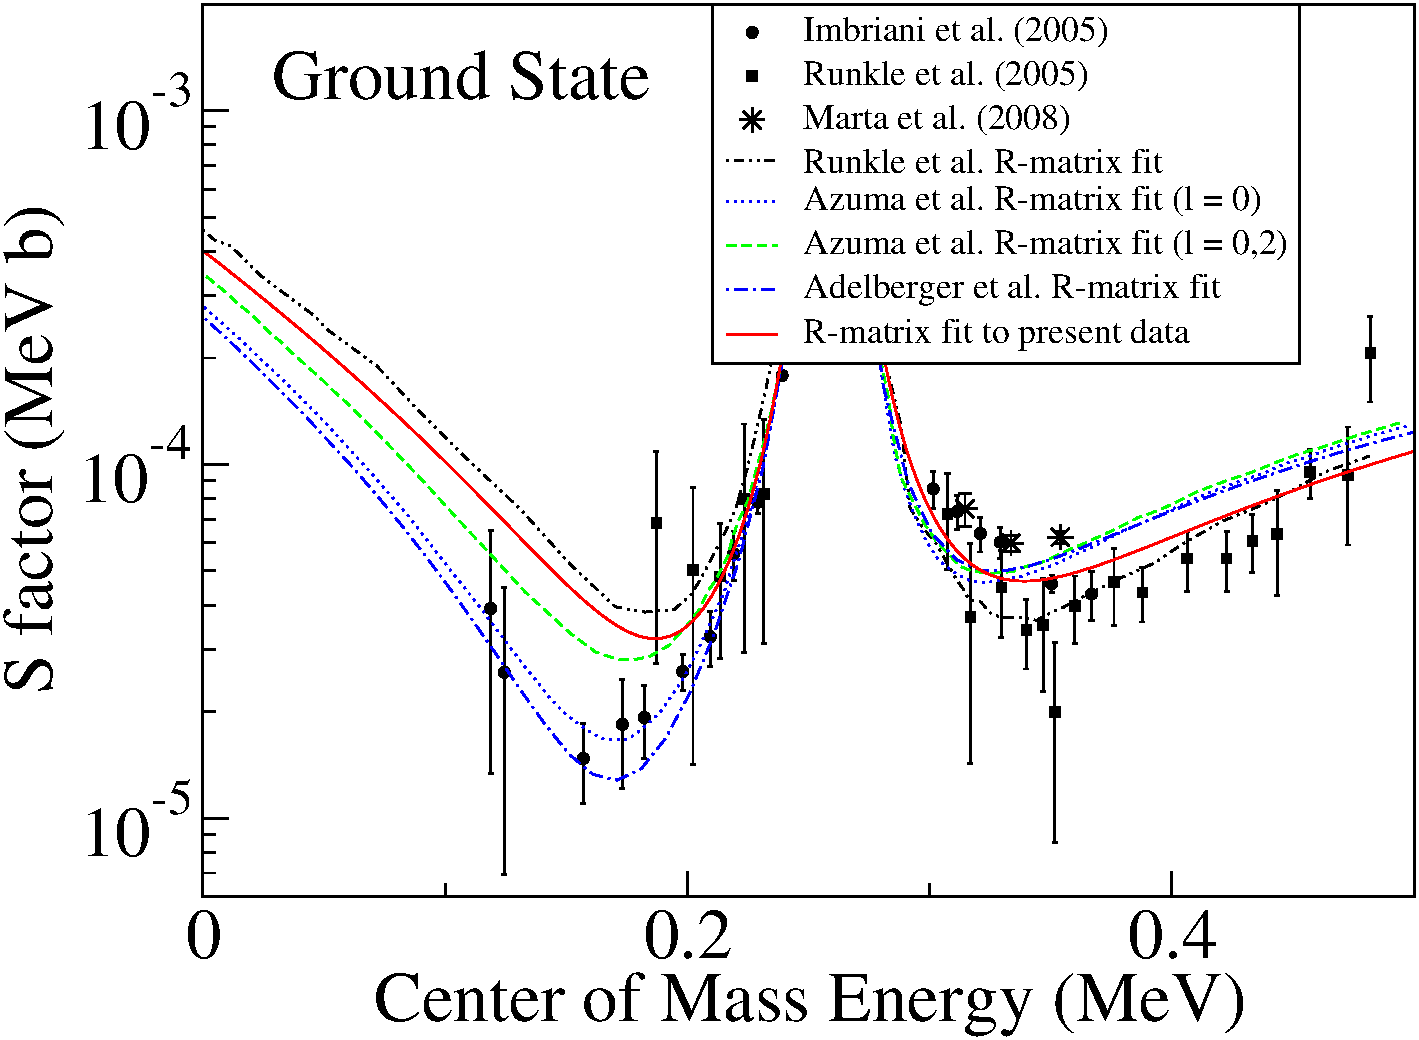
\includegraphics[width=\linewidth]{figures/qianSfactor.pdf}
\caption{$R$-matrix extrapolation of the $S$-factor given in \cite{Li2016}. The authors identified the major sources of uncertainty as the uncertainty as the DC/R$\rightarrow$gs primary transition, the DC/R$\rightarrow$6.17 MeV level primary transition, and the $\Gamma$ width of the 6.79 MeV state. Of these, the latter is the dominant term. This figure highlights the effects that these uncertainties have on low-energy extrapolations, varying by nearly a factor of two. }
\label{fig: QianRmatrix}
\end{figure}

The Wagner \textit{et al.} study attempted to remedy this, providing an independent cross check of the ground state and 6.79 MeV capture transitions in the proton energy range of $E_{p}$ = 366–1289 keV, overlapping with the low-energy data sets. In the study, the authors found $S$-factors elevated significantly above those of any previous measurement for both of the transitions measured. Due to this, their results for the extrapolated $S(0)$ and contributions from the DC/R$\rightarrow$6.79 MeV transition agree with those from Li \textit{et al.}, but they are unable to draw conclusions about the ground state transition or any of the other, weaker transitions. Ultimately, this means that their results were unable to address any of the major uncertainties left plaguing the situation. 



\subsection{Lifetime}
\label{sec: lifetimeLiterature}


The $\Gamma$ width of the 6.79 MeV subthreshold state is the dominant uncertainty on the total $S$-factor at zero energy, as illustrated by Fig. \ref{fig: QianRmatrix}. The literature to date on the lifetimes/widths of the important levels in $\ce{^{15}O}$ are summarized in Table \ref{table: lifetimes}. Some of the values present in the table are those extracted as a fit parameter from $R$-matrix analyses, instead of experimental measurements \cite{Schroder1987, Angulo2001, Formicola2004, Runkle2005, Marta2008, Azuma2010, Adelberger2011b}. By having a dominant term of the calculation be a floating fit parameter, accuracy and reliability in the extrapolations are lost. Therefore, determination of this quantity experimentally is critical. 


\begin{table}[]
\thisfloatpagestyle{plain}
\caption{SUMMARY OF PREVIOUS LIFETIME/WIDTH MEASUREMENTS FOR IMPORTANT STATES IN $^{15}$O}
\centering
\begin{threeparttable}
\begin{tabular}{lllll}
\hline
                                                   & $\tau_{6.79}$ fs       & $\tau_{6.17}$ fs       & $\tau_{5.18}$ fs      & $\Gamma^{6.79}$ (eV)    \\ \hline
Gill \textit{et al.} \cite{Gill1968}               & $< 28$                 & $< 2.5$                & 8.2 $\pm$ 1.0         & $--$                    \\
Schr{\"o}der \textit{et al.} \cite{Schroder1987}   & $--$                   & $--$                   & $--$                  & 6.3                     \\
Bertone \textit{et al.}$^{a}$ \cite{Bertone2001}   & $1.60^{+0.75}_{-0.72}$ & $2.10^{+1.33}_{-1.32}$ & $9.67^{+1.34}_{1.24}$ & $0.41^{+0.34b}_{-0.13}$ \\
Angulo \textit{et al.} \cite{Angulo2001}           & $--$                   & $--$                   & $--$                  & 1.75 $\pm$ 0.60$^{c}$   \\
Yamada \textit{et al.} \cite{Yamada2004}           & $0.69^{+1.10}_{-0.69}$ & $--$                   & $--$                  & $0.95^{+0.60}_{-0.95}$  \\
Formicola \textit{et al.} \cite{Formicola2004}     & $--$                   & $--$                   & $--$                  & 0.8 $\pm$ 0.4$^{c}$     \\
Sch{\"u}rmann \textit{et al.}$^{b}$ \cite{Schurmann2008} & $< 0.77$               & $< 0.77$               & 8.4 $\pm$ 1.0         & $> 0.85$                \\
Azuma \textit{et al.} \cite{Azuma2010}             & $--$                   & $--$                   & $--$                  & 2.38$^{c}$              \\
Adelberger \textit{et al.} \cite{Adelberger2011}   & $--$                   & $--$                   & $--$                  & 3.25$^{c}$              \\
Michelagnoli$^{a,d}$ \cite{Michelagnoli2013}        & $< 1.0$                & $--$                   & $--$                  & $> 0.66$                \\
Galinski \textit{et al.}$^{b}$ \cite{Galinski2014}  & $< 1.8$                & $< 2.5$                & $--$                  & $> 0.44$                \\ \hline
\end{tabular}
\begin{tablenotes}
\small 
\item A summary of previous lifetime/width measurements for important states in $\ce{^{15}O}$. a) Measurements reported with 90\% confidence limit. b) Measurements reported with 68.3\% confidence limit. c) Reported value calculated from $R$-matrix analysis. d) Reported in Ph.D. thesis, not peer reviewed.
\end{tablenotes}
\end{threeparttable}
\label{table: lifetimes}
\end{table}

There are only five measurements of the lifetime or width of the 6.79 MeV state ''directly'' \cite{Bertone2001, Yamada2004, Schurmann2008, Galinski2014, Michelagnoli2013}, highlighted in red in Table \ref{table: lifetimes}, and they are unfortunately disparate in their extracted values and have relatively large errors. This is primarily due to the difficulty in measuring the lifetime, thought to be below one femtosecond, and at the edge of the feasibility of current techniques. Four of the measurements \cite{Bertone2001, Schurmann2008, Galinski2014, Michelagnoli2013} performed the measurement by the Doppler Shift Attenuation Method (DSAM) while the other used Coulomb Excitation to measure the state's width.

The first measurement was performed in 2001 by Bertone \textit{et al.}, using the DSAM to determine the lifetime of the state. This technique will be discussed in further detail later. The authors populated the state through resonant capture of protons in the $E_{p}$ = 278 keV state and observed the decaying $\gamma$-rays at three different angles. The measured lifetime for the 6.79 MeV state was determined to be $\tau = 1.60^{+0.75}_{-0.72}$ fs, corresponding to a width of $\Gamma = 0.41^{+0.34}_{-0.13}$ eV (determined by Equation \ref{eqn: width to lifetime}), where the uncertainties reported correspond to a 90\% confidence limit. 

At RIKEN, in 2004, Yamada \textit{et al.} performed a measurement of the radiative width via Coulomb Excitation experiment \cite{Yamada2004} as an independent verification of the Bertone result. For this, $\ce{^{15}O}$ nuclei were produced by fragmentation of an $\ce{^{16}O}$ beam incident on a $\ce{^{9}Be}$ target and then inelastically scattered off of a thick lead target. The de-excitation $\gamma$-rays were detected with an array of NaI (Tl doped) scintillation detectors. In order to disentangle the 6.79 MeV peak of interest from the 6.86 MeV peak in their spectrum, the authors compared the experimentally obtained spectrum from with the results of a Monte Carlo simulation. Due to the poor energy resolution of the detector system, the authors ultimately had difficulty separating the peaks and only reported an upper bound on the width, $\Gamma = 0.95^{+0.60}_{-0.95}$ eV, and a corresponding lifetime of $\tau = 0.69 ^{+1.10}_{-0.69}$ fs. 

Four years later, Sch{\"u}rmann \textit{et al.} published a new measurement of the lifetime using the DSAM technique and an improved experimental setup \cite{Schurmann2008}. This measurement used a single high-purity germanium (HPGe) detector on a rotating track and measuring at many more angles ranging from $40 - 116^{\degree}$, allowing for a check of asymmetries around the $90^{\degree}$ point and reducing systematic uncertainties from the use of different detectors. Similar to the Bertone measurement \cite{Bertone2001}, the authors populated the state of interest via the resonance at $E_{p} = 278$ keV in the $^{14}$N$\left( p,\gamma \right) ^{15}$O reaction. In contrast to the Bertone result and similar to the Yamada work, the authors in this case could not recommend a finite value for the measured lifetime, obtaining a lifetime upper limit of $\tau < 0.77$ fs, also to 68.3\% confidence. 

In another attempt to determine the lifetime, Galinski \textit{et al.} performed another DSAM measurement at the TRIUMF facility \cite{Galinski2014}. The major difference this time, however, was that the reaction occurred in inverse kinematics (i.e. one where the heavier reaction input is accelerated towards the stationary, lighter one), emulating a result from over 50 years ago \cite{Gill1968}. The $\ce{^{15}O}$ in this experiment were produced via the $\ce{^{3}He}(\ce{^{16}O},\alpha)\ce{^{15}O}$ reaction with a $\ce{^{3}He}$-implanted gold-foil and the de-excitation $\gamma$-rays were detected with a clover HPGe detector (a single detector containing four separate Ge crystals) and filtered in coincidence with the reaction product $\alpha$'s. The authors performed a Bayesian line-shape analysis of the spectra and could not find a definite lifetime. As such, the authors recommended upper limit given by experimental uncertainties of $\tau < 1.8$ fs with a 68.3\% confidence limit. The authors, however, acknowledge that their result was statistics limited.

The final measurement of this lifetime comes from an unpublished doctoral dissertation by Michelagnoli in 2013 \cite{Michelagnoli2013}. Similar to Galinski \textit{et al.}, this measurement was done in inverse kinematics, with the $d(\ce{^{14}N},\ce{^{15}O})n$ reaction. The $\gamma$ rays from this measurement were detected with the state-of-the-art AGATA Demonstrator array using $\gamma$-ray tracking for precision angular data and a lineshape analysis of the data was performed by comparing with the results of a Monte Carlo simulation in the Geant4 software. This work also obtained only an upper-bound on the lifetime, $\tau < 1.0$ fs with a 68.3\% confidence limit. While this result is consistent with other literature values, it should nonetheless be taken with a grain of salt as it has not been peer-reviewed. 

In aggregate, these results are unsatisfactory, with an error that is still uncomfortably large. Particularly, the DSAM results (with the exception of Galinski \cite{Galinski2014}) neglected the systematic uncertainties from the stopping power of the targets in their ultimate lifetime calculation. The forward kinematics reactions \cite{Bertone2001, Schurmann2008} both used nitrogen-implanted tantalum-foils for the experiment (saturated to a composition of Ta$_{2}$N$_{3}$), but calculated the lifetimes assuming target densities and stopping powers equal to those of pure tantalum, calculated in SRIM \cite{Ziegler2010}. However, in this lifetime range, the deceleration of the $\ce{^{15}O}$ nuclei occurs in the region where the nitrogen is present in the lattice. Specifically, this means that the presence of the nitrogen has a significant effect on the actual stopping power. According to the authors of the respective works, the inclusion of accurate densities and stopping powers would have changed the inferred lifetimes of their works by 100\% \cite{Bertone2001} and 2\% \cite{Schurmann2008}, respectively. In both, the authors also independently measured the lifeitme of the 5.18 MeV state, with results agreeing with other literature values. Because of this, both sets of authors contend that their calculations are appropriate and accurate, which is a clear contradiction.





\section{Objective}
\label{sec: thesis outline}

The results of a series of experiments and subsequent analyses performed to better understand the low energy behavior of the $^{14}$N$\left( p,\gamma \right) ^{15}$O will be presented herein. These include the measurement of the $^{14}$N$\left( p,\gamma \right) ^{15}$O reaction at energies between 270 keV and 1200 keV undertaken at both the University of Notre Dame Nuclear Science Laboratory (NSL) and the Compact Accelerator System for Performing Astrophysical Research (CASPAR), located in the Sanford Underground Research Facility in the renovated Homestake Gold Mine in South Dakota. Additionally, a measurement of the lifetime of the 6.79 MeV level in $^{15}$O also at the NSL is also included in this work. These data will then be used in an $R$ Matrix calculation to provide a new determination of the $^{14}$N$\left( p,\gamma \right) ^{15}$O reaction rate.

The experimental techniques used in these measurements is presented in Chapter \ref{chap: experiment}, including specific details about each phase of the measurement. There is a brief overview of the standard equipment common to each of the measurements. Following this, the specific features of the different types of measurements and the facilities in which they were made will be presented in further detail. 

Chapters \ref{chap: data} - \ref{chap: lifetime} will present details on the different facets of the data reduction and analysis. The first of these, Chapter \ref{chap: data}, shows the data for $^{14}$N$\left( p,\gamma \right) ^{15}$O taken at the NSL and CASPAR while detailing the process by which the cross-section and astrophysical $S$-factor were extracted. Chapter \ref{chap: lifetime} focuses on the nuclear lifetimes, describing the codes that were developed and used to analyze the Doppler Shift in the $\gamma$-ray data to determine the lifetime of the states in $^{15}$O. The validity of the method is checked against other known $^{15}$O levels populated in the reaction, like the states at 5.18 MeV and 6.17 MeV, respectively.

The cross-section information and newly measured lifetime will be utilized in a new $R$-matrix analysis of the $^{14}$N$\left( p,\gamma \right) ^{15}$O reaction, presented in Chapter \ref{chap: r-matrix}. The new constraints these data provide on the low-energy behavior of the extrapolated $S$-factor will be provided, alongside a description of their impact to relevant astrophysical quantities.

Finally, Chapter \ref{chap: conclusions} presents an overview of the respective impacts of the measurements paired with future outlook. 

% % uncomment the following lines,
% if using chapter-wise bibliography
%
% \bibliographystyle{ndnatbib}
% \bibliography{example}



%
% Chapter 2
%

%
% Modified by Megan Patnott
% Last Change: Jan 18, 2013
%
%%%%%%%%%%%%%%%%%%%%%%%%%%%%%%%%%%%%%%%%%%%%%%%%%%%%%%%%%%%%%%%%%%%%%%%%
%
% Modified by Bryce Frentz
% Last Change: 2018
%
%%%%%%%%%%%%%%%%%%%%%%%%%%%%%%%%%%%%%%%%%%%%%%%%%%%%%%%%%%%%%%%%%%%%%%%%
%
% Sample Notre Dame Thesis/Dissertation
% Using Donald Peterson's ndthesis classfile
%
% Written by Jeff Squyres and Don Peterson
%
% Provided by the Information Technology Committee of
%   the Graduate Student Union
%   http://www.gsu.nd.edu/
%
% Nothing in this document is serious except the format.  :-)
%
% If you have any suggestions, comments, questions, please send e-mail
% to: ndthesis@gsu.nd.edu
%
%%%%%%%%%%%%%%%%%%%%%%%%%%%%%%%%%%%%%%%%%%%%%%%%%%%%%%%%%%%%%%%%%%%%%%%%

%
% Chapter 2
%

\chapter{Experimental setup and procedures}
\label{chap: experiment}

\section{Introduction}

This chapter is included to highlight some techniques and equipment commonly used in low-energy nuclear physics, with an emphasis on those used in this work. The discussion will be presented from the lens of the general to the specific, introducing general concepts for beam production and transport, acceleration systems, and radiation detection. Following the discussion of the scientific principles, I will detail the specifics of the equipment employed in this collective work. To that end, I will also highlight differences between the facilities and techniques employed when compared to common equipment for nuclear physics experiments


\section{Experimental Equipment}
\label{sec: equipment}



\subsection{Accelerators}
\label{sec: accelerators}

First and foremost, low-energy nuclear physics (generally understood to be the regime in which incident kinetic energies for reactions are below 1 GeV, often even as low as sub-MeV) requires particle acceleration systems in order to bring beams and targets together. The most common techniques for accelerating ions are 1) to use strong electrostatic fields for a straight-line acceleration, such as in the Van de Graaff accelerator, or 2)  by using a combination of electric and magnetic fields to accelerate the particles in cyclotron motion, aptly named a cyclotron. Van de Graaff accelerators are the most prominent of all accelerators, though, and are the type used in this work. 

The basic idea of a Van de Graaff accelerator is shown in Fig. \ref{fig: vdg principles}. The governing principle is that a beam of ions produced in an ion source (Section \ref{sec: ion sources}) are manipulated by additional electromagnetic elements (Section \ref{sec: beamline}) into an area of high electric potential. This high voltage is produced and maintained by continuously transporting positive charge from ground to a Faraday cage with a field free interior (referred to as the terminal, with voltage $V_{T}$). The positively charged ions, being in close proximity to the positively charged terminal feel a repulsive force, accelerating the ions out of the terminal and through the machine. Upon exiting the accelerator, the ions have energy

\begin{equation}
E_{ion} = qV_{T} = \dfrac{1}{2} m_{ion} v_{ion}^{2}
\label{eqn: accelerator}
\end{equation}

\noindent where $V_{T}$ again is the terminal voltage and $q$ is the charge state of the ion going through the accelerator, $m_{ion}$ is the mass of the ion, and $v_{ion}$ is the ion's velocity. When the terminal voltage is in MV, the beam energy is then provided in MeV. Specifically for the 5U accelerator, though, Equation \ref{eqn: accelerator} must be modified with an additional term. Inside the ion source, there is an electrostatic extractor, which transports the beam of ions out of the terminal and into the acceleration tube. With this correction, the beam energy for the 5U is given as

\begin{equation}
E_{ion} = q(V_{extractor} + V_{T}).
\label{eqn: beam energy}
\end{equation}

\begin{figure}
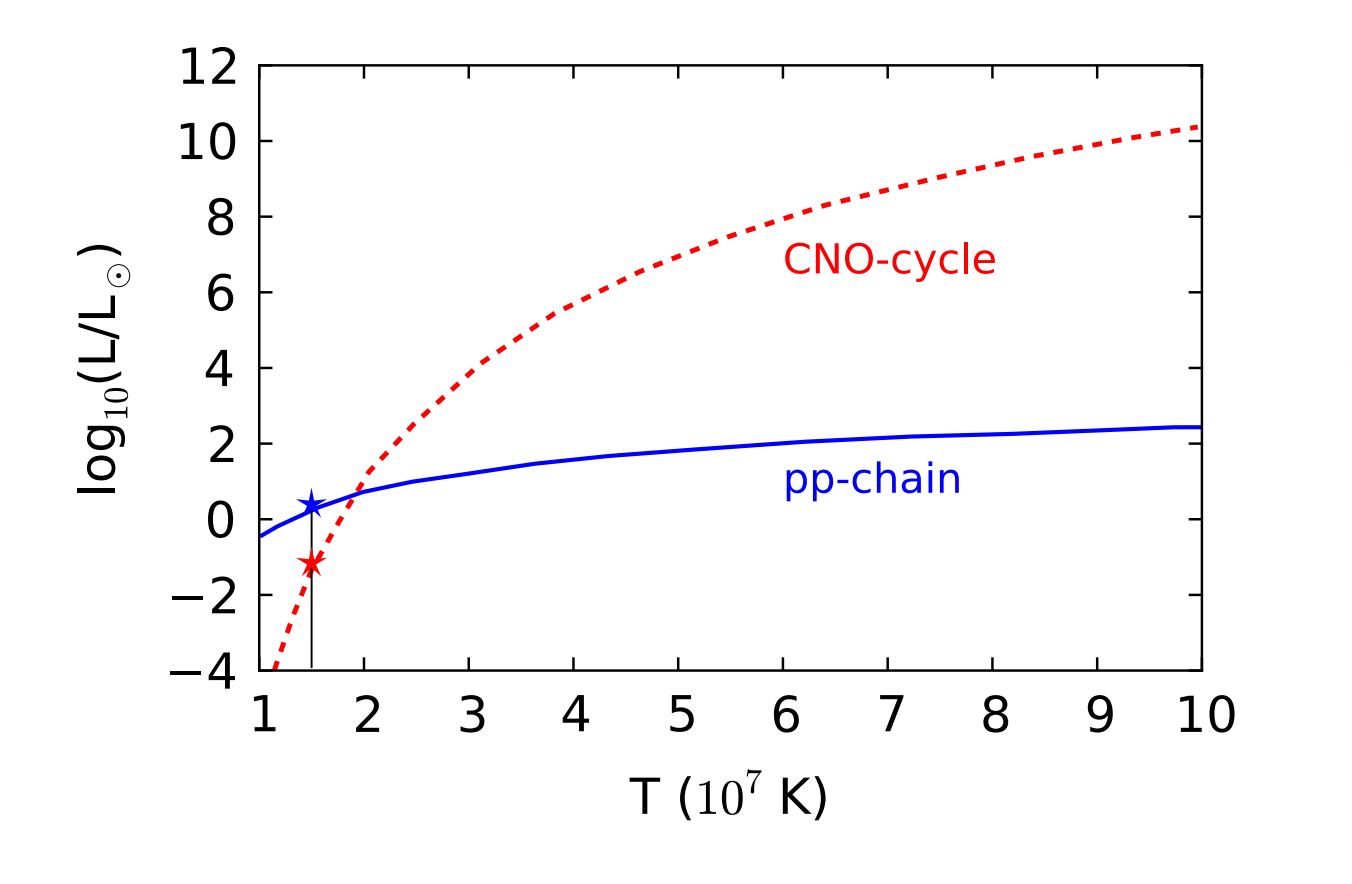
\includegraphics[width=\linewidth]{figures/energyProduction.png}
\label{fig: vdg principles}
\caption{A diagram of a Van de Graaff accelerator \cite{RolfsBook}. The charge transportation in this figure is shown with a belt, like the JN accelerator model at CASPAR, while the 5U accelerator at the NSL uses a Pelletron chain. }
\end{figure}

The charge is delivered to the terminal via a mechanical delivery system. The 5U Sta. Ana accelerator at the NSL uses four Pelletron chains cite{Herb1974}, each with its own power supply, while the JN Van de Graaff accelerator at CASPAR utilizes a rotating belt. In either case, the entire charging system is contained inside of a pressurized tank of insulating gas, SF$_{6}$ for the 5U and CO$_2$ for the JN, reducing the chance of a terminal discharge to ground from dielectric breakdown. This is not the only element to ensure the operational stability of the machine. The charging systems supply charge continuously to the terminal. However, charge is always being removed from the terminal via three primary pathways: 1) the beam of ions passing through the accelerator, 2) the resistive column, and 3) the corona system. In order to maintain stability, the currents that pass through these systems must always be in balance according to Kirchoff's Rule,

\begin{equation}
I_{chains} = I_{beam} + I_{column} + I_{corona}.
\end{equation}

\noindent The column is actually a series of equipotential hoops connected by equal resistors. Each conducting hoop provides a small step down in voltage from the terminal, ensuring that the beam of ions feel a smooth potential gradient throughout their acceleration. These can be seen in Fig. \ref{fig: column}, showing an interior view of Sta. Ana accelerator tank. 


\begin{figure}
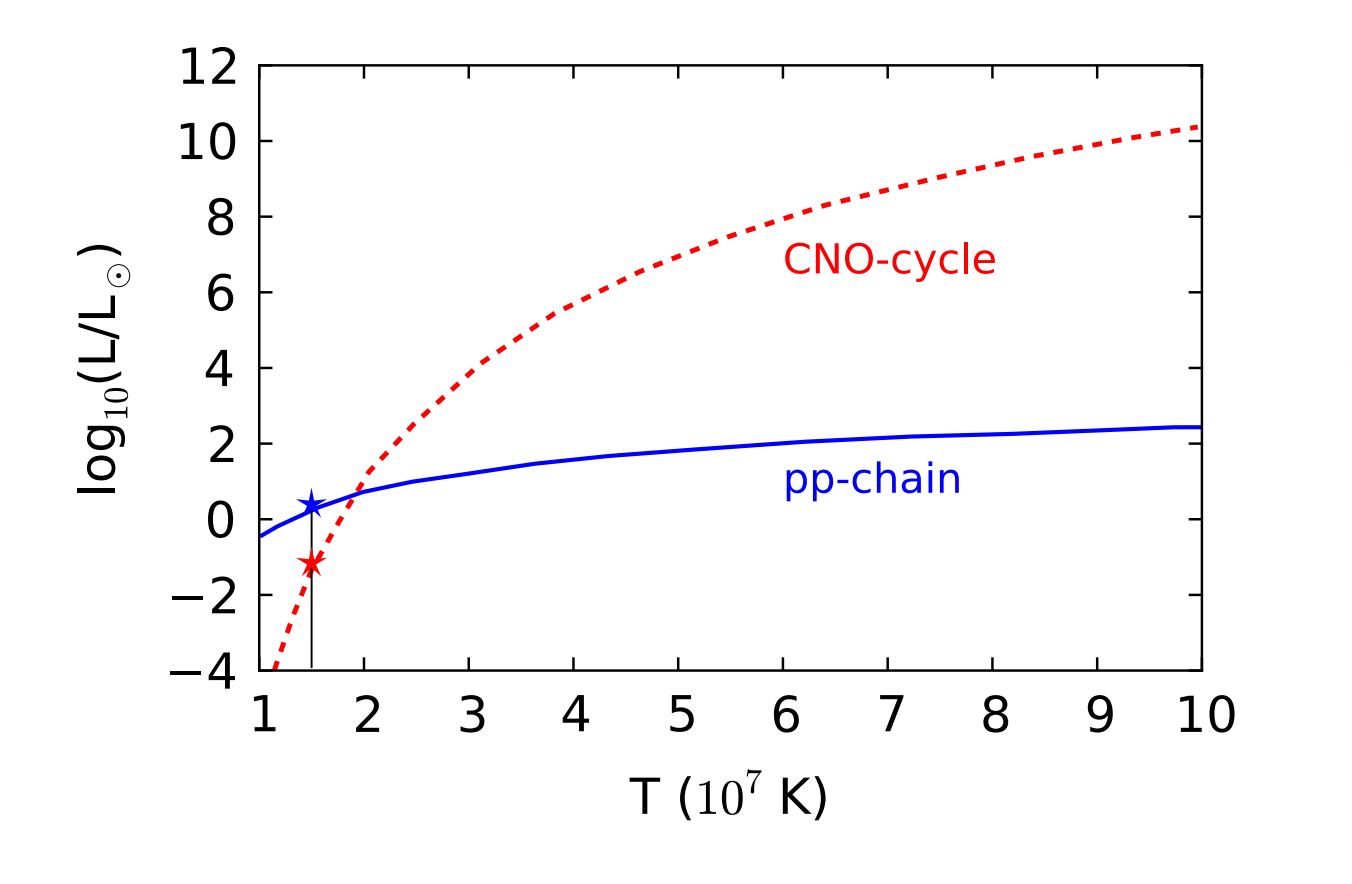
\includegraphics[width=\linewidth]{figures/energyProduction.png}
\label{fig: column}
\caption{View inside the Sta. Ana accelerator tank, showing the equipotential hoops as part of the column.}
\end{figure}


The corona system is the real workhorse maintaining the stability of the accelerator's charging systems. As small irregularities can be present between different links in the Pelletron chains or the belt itself, the corona system is responsible for precise second-by-second compensation. The mechanical part of the system consists of an arm with sharp metal points on the end which can be moved towards and away from the terminal to draw away current. On the back end, however, it also is controlled by a voltage feedback system to adjust the current draw, keeping the terminal at a constant voltage. The feedback for the system is provided either by an external reference through a generating voltmeter or from the beam itself as it passes through an analyzing dipole magnet at the exit of the accelerator. As the beam passes through the magnet it will pass through a set of slits. If $V_{T}$ changes slightly, the energy of the beam will subsequently change, impacting the balance of the beam on the exit slits. This change in current will be fed back to the corona system, which in turn will compensate by changing the charge delivered to the terminal in order to maintain the slit balance. With this, $V_{T}$ can be kept incredibly steady, within roughly 1 kV for every MV on the terminal. This is the biggest advantage of a Van de Graaff accelerator over a cyclotron. Intrinsically, this acceleration system makes nuclear experiments possible through monoenergetic beams. 


\subsection{Ion sources}
\label{sec: ion sources}

A key item for the successful operation of any accelerator is the ion source, which produces the beams of charged particles used in experiments. Generating such beams is not a trivial task and, as such, many methods have been developed for achieving this. The two types relevant to this work, however, are the Electron-Cyclotron Resonance (ECR) ion source, used in the Sta. Ana accelerator at the NSL, and the radio frequency (RF) ion source, utilized in the JN accelerator at CASPAR.  Both systems are housed within their respective accelerator terminals, which acts as a Faraday cage and shields the internal components from external fields. Additionally, both systems operate on the same basic principle, namely that a given gas is ionized through the use of electron collisions in the source, but the mode of electron excitation is different. 

For the specifics of the ECR system, the 5U employs a Pantechnik Nanogen 14.5 GHz ECR source. This utilizes the cyclotron resonance of electrons (as the name obviously implies) to produce and maintain a plasma.


\begin{figure}
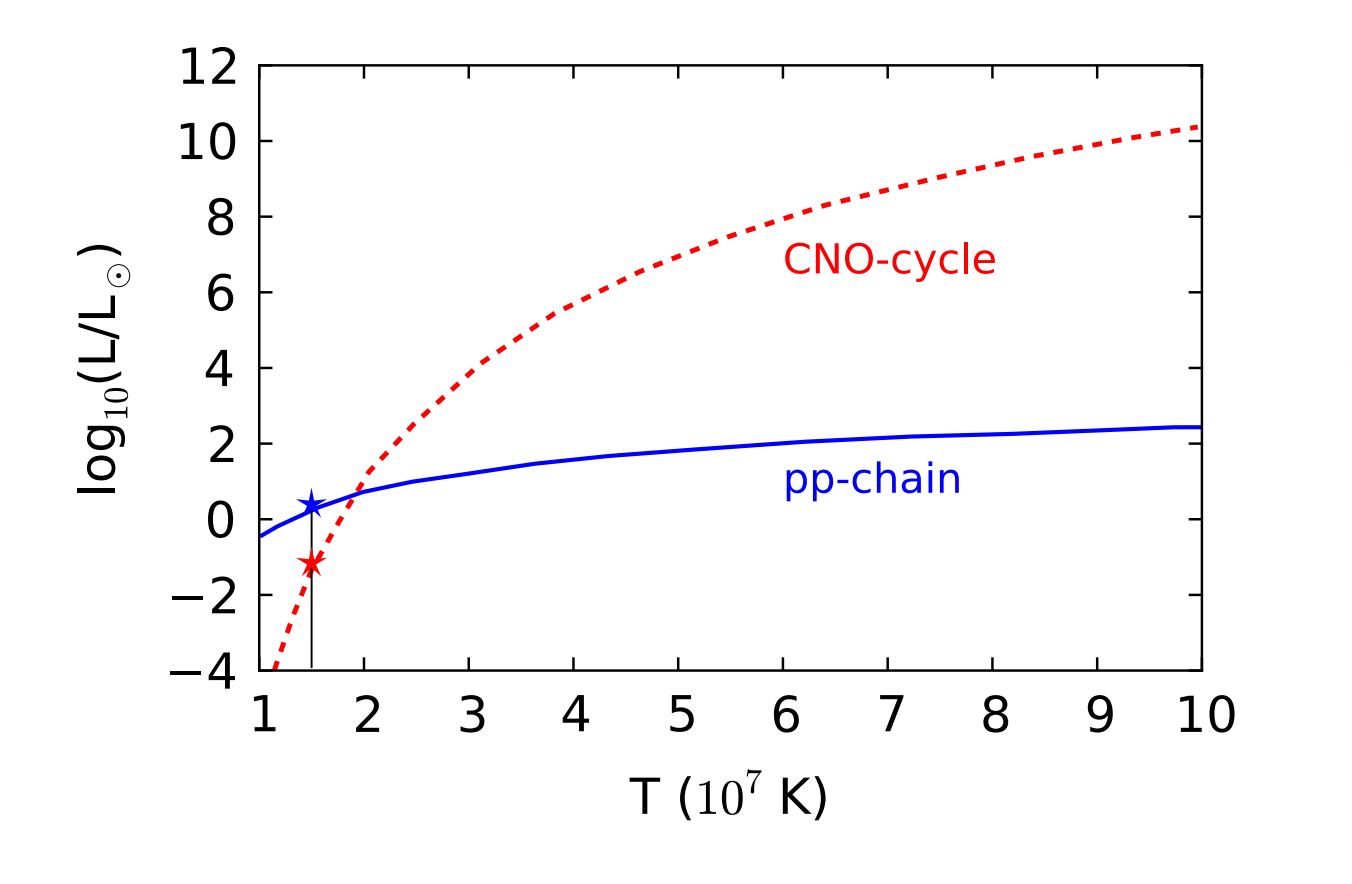
\includegraphics[width=\linewidth]{figures/energyProduction.png}
\label{fig: ecris}
\caption{Depiction of the interior of an ECR ion source with magnetic components labeled cite{Melin1997}. This example shows a source operating from left to right, with the gas and RF generator inputs depicted as well as the exit for the ions. As discussed in the text, the combination of magnets confines the plasma in the center as it is pushed from left to right and out of the source.}
\end{figure}


During operation, neutral gas (which includes the element to be accelerated as a component) is injected into a cavity surrounded by magnets. These magnets provide a superposition of axial and multipole fields in order to achieve a minimum at the center of the cavity increasing radially outwards with the goal of confining and stabilizing the generated ions. A cartoon depiction of such a system is presented in Fig. \ref{fig: ecris}. In order to generate the ions from neutral gas, a current is supplied to the chamber by a negative bias probe providing a constant supply of charge. From this, then, electrons are stripped and continually accelerated in cyclotron motion following the familiar cyclotron frequency relation:

\begin{equation}
\omega_{ecr} = \dfrac{e | B |_{ECR}}{m_{e}} = \omega_{rf}
\label{eqn: ecr}
\end{equation}

\noindent where $\omega_{ecr}$ is the frequency for the cyclotron resonance of electrons in a given magnetic field $B_{ECR}$, $e$ and $m_{e}$ are the charge and mass of the electron, respectively, and $\omega_{rf}$ is the frequency supplied by a radio radio-frequency (RF) power supply. This last term is included to highlight that during operation this is supplied externally and controlled in the use of the source in order to produce the plasma. After ionization, the magnetic configuration confines the plasma radially, while the axial magnetic field (provided by the extractor) pushes it through the cavity towards the exit of the source. Upon exiting the chamber and the Faraday cage of the terminal, the positive ions are next to a the positively charged terminal at high voltage, thus accelerating the ions. 

An ECR ion source has many advantages of over other common ion source designs. The primary advantage lies in its ability to deliver high-intensity beams (as much as hundreds of $\mu A$). For use in nuclear astrophysics experiments, such as the ones performed in this work, low cross sections are a problem to overcome, which is mitigated through this higher production. Additionally, due to the relatively simple restrictions on the inputs, these sources can provide a wide array of species, as they can produce beams of nearly anything that can be made into a gas, and exhibit long term stability, reliability, and longevity cite{Melin1997}.  On the other hand, however, ECR ion sources also have some disadvantages compared to other common sources. One main drawback is that the ions are produced through the production of a plasma, meaning they are not directly controlled by any operational parameter cite{Melin1997}. This leads to complicated tuning and sensitive operation, experimentally. Additionally, such sources are only capable of generating positive beams and can therefore only be utilized in single stage accelerators. Finally, due to the size of these ion sources and their necessary components, they are often impractical. In order to employ one in the Sta. Ana accelerator, the accelerator design had to be vertical. If the accelerator had been horizontal (like the other accelerators at the NSL) the torque generated by the ECR ion source would have shattered the acceleration column. Vertically, however, the source is stable inside the accelerator. Unfortunately, the choice to build and use the accelerator vertically is not one that every lab can make. 

The radio frequency (RF) ion source utilized at CASPAR operates on a very similar principle to the ECR ion source inside the Sta. Ana accelerator. A depiction of the RF ion source's components is given in Fig. \ref{fig: rfis}. In this case, the source chamber is a glass tube filled with a monoatomic gas, at CASPAR the only options are $\ce{^{1}H}$ and $\ce{^{4}He}$.  Electromagnetic coils are placed on both sides of this tube and generate RF waves in the tube, between the rings. In response to these waves, the electrons oscillate through and collide with the source gas, ionizing it. At the rear of the glass tube, an electrode supplies a constant, positive voltage (with respect to the terminal), forcing any ionized atoms towards the exit of the source. Upon leaving the source, as with the ECR ion source, the ions are accelerated because of their repulsion to the positively charged terminal. 

\begin{figure}
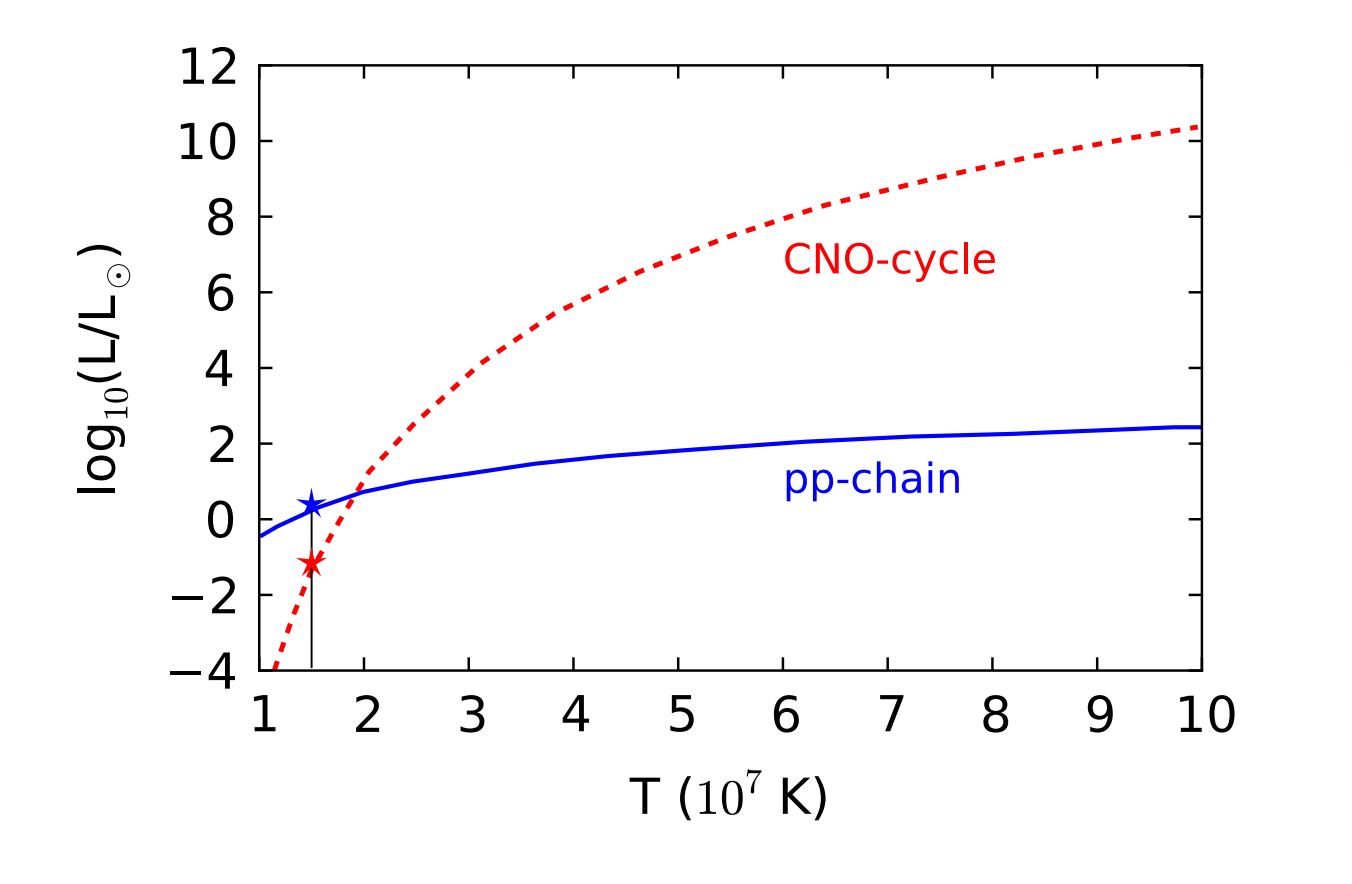
\includegraphics[width=\linewidth]{figures/energyProduction.png}
\label{fig: rfis}
\caption{Depiction of the interior of a RF ion source with magnetic components labeled cite{Li2015}. The coils on either side provide the field to ionize the gas, whereas the probe on top provides the field necessary to extract the ions from the chamber.}
\end{figure}

The RF ion source at CASPAR was also recently refurbished before installation, leaving it capable of beam production at even higher intensities than the ECR ion source inside the Sta. Ana accelerator. It can produce beams up to 150 $\mu A$, enabling similar high-intensity experiments. Another similarity to the ECR ion source is that it provides excellent operational stability and reliability. It does, however have significant drawbacks as well. The first and foremost of these is the degredation of the ion source canal. Operating the source causes a buildup on the exit canal of the source tube (higher intensity operation accelerates this process), necessitating significant maintenance. Additionally, the glass tube housing the plasma is quite sensitive. If power is supplied to the source when gas is not present, significant damage to the tube can occur. This is only mitigated with vigilant operation. The other major drawback is that the source is only capable of providing beams of two species (typically hydrogen and helium). In order to change the delivered species, a full tank opening and source alignment is required. 

Altogether, though, these sources are ideal for this work. They provide the necessary ion beams at high intensity, enabling the experiments. 




\subsection{Beam transport}
\label{sec: beamline}


Upon exiting the accelerator, the beam envelope contains a distribution of different masses, charges, and energies because the ion sources are indiscriminate in their production methods. For example, an ion source might produce some ionized diatomic gas, instead of monoatomic, like producing $\ce{^{1}H}+\ce{^{1}H}$ due to insufficient breakup of the source gas. However, all particles created in the same ionization state will have the same energy, dictated by Equation \ref{eqn: beam energy}. In order to filter such contaminants out of the beam, analyzing magnets are employed. These are typically 90$^{\deg}$ dipole magnets, also utilizing the cyclotron motion of ions in a magnetic field in order to select a given type of particle at a specific energy. These magnets are typically located at the exit of accelerators, and, due to their fixed size, have a fixed radius, $R_{am}$, through which a beam can pass. Therefore, for a given particle of mass $m$, energy $E$, and charge state $q$, the magnetic field, $B_{am}$, inside the analyzing magnet can be tuned to allow through only a specific particle/energy combination by

\begin{equation}
B_{am} = \dfrac{\sqrt{2 m E}}{q R_{am}} = \dfrac{\sqrt{2m}}{q R_{am}} \sqrt{E} = k \sqrt{E}
\label{eqn: analyzingMagnet}
\end{equation}

\noindent, where $k$ is a constant for a unique combination of particle and charge state. This separates the in-beam contaminants from the ions of experimental interest.  

In order to deliver the beam of ions to the target chamber and experimental hall, a series of steering and focusing elements are placed along the beam pipes. As the beam is self-repulsive due to it all being the same charge, these are necessary to contain the beam and keep its intensity at acceptable levels for experimental purposes. They also allow adjustment of the beam's position in order to deliver it to a specific experimental setup and allowing for simple transitions between different target locations. 

Vacuum systems are important components of the beam production and experimental operation. All experimental components, like the ion source chamber, acceleration tubes, target chamber, and connecting beam pipes need to be free of residual gas. If not, the beam quality would suffer dramatically, collisions of the beam with the remaining atmosphere would cause significant intensity and energy losses, preventing transport and, ultimately, the measurement. In order to maintain an experimental vacuum level (typically $\sim 10^{-7}$ Torr), a series of metal pipes run from the ion source to the target chamber. These are connected by air-tight gaskets and have isolating valves employed with high-vacuum pumps (cryogenic or turbomolecular) along the line. These enable easier maintenance or changing of experimental conditions without destroying the vacuum created through the entire beam line. Without high-vacuum, there would be additional adverse effects on the target quality. Contaminants, typically hydrocarbons, present in residual gas can accumulate on the surface of the target due to the beam heating the surface. This is unwanted, as it not only provides an additional layer of energy loss for the beam before interacting with the target but also a significant contaminant in experimental results due to carbon's high cross-section.

Besides maintaining clean, high-vacuum near a target, another common method for reducing the carbon build-up on experimental surfaces is to utilize a so called cold trap in front of a target. A cold trap is is a liquid nitrogen cooled copper pipe designed to be nearly the same size and shape as the beam pipe to prevent it from interfering with an experiment. An example of a cold trap like the one used in this work is shown in Fig. \ref{fig: setup}. The cold trap works much like a cryogenic pump. By cooling the copper pipe with liquid nitrogen, the residual hydrocarbons in the beam pipe and target chamber will condense on the surface of the pipe, trapping them before most can reach the target and cause carbon buildup. A common practice, which we also employed in this work, is to apply a negative voltage to the cold trap, forcing electrons scattered by the collision of the beam with the target back to the end of the chamber and providing an accurate reading of the amount of beam delivered to the target. 


\begin{figure}
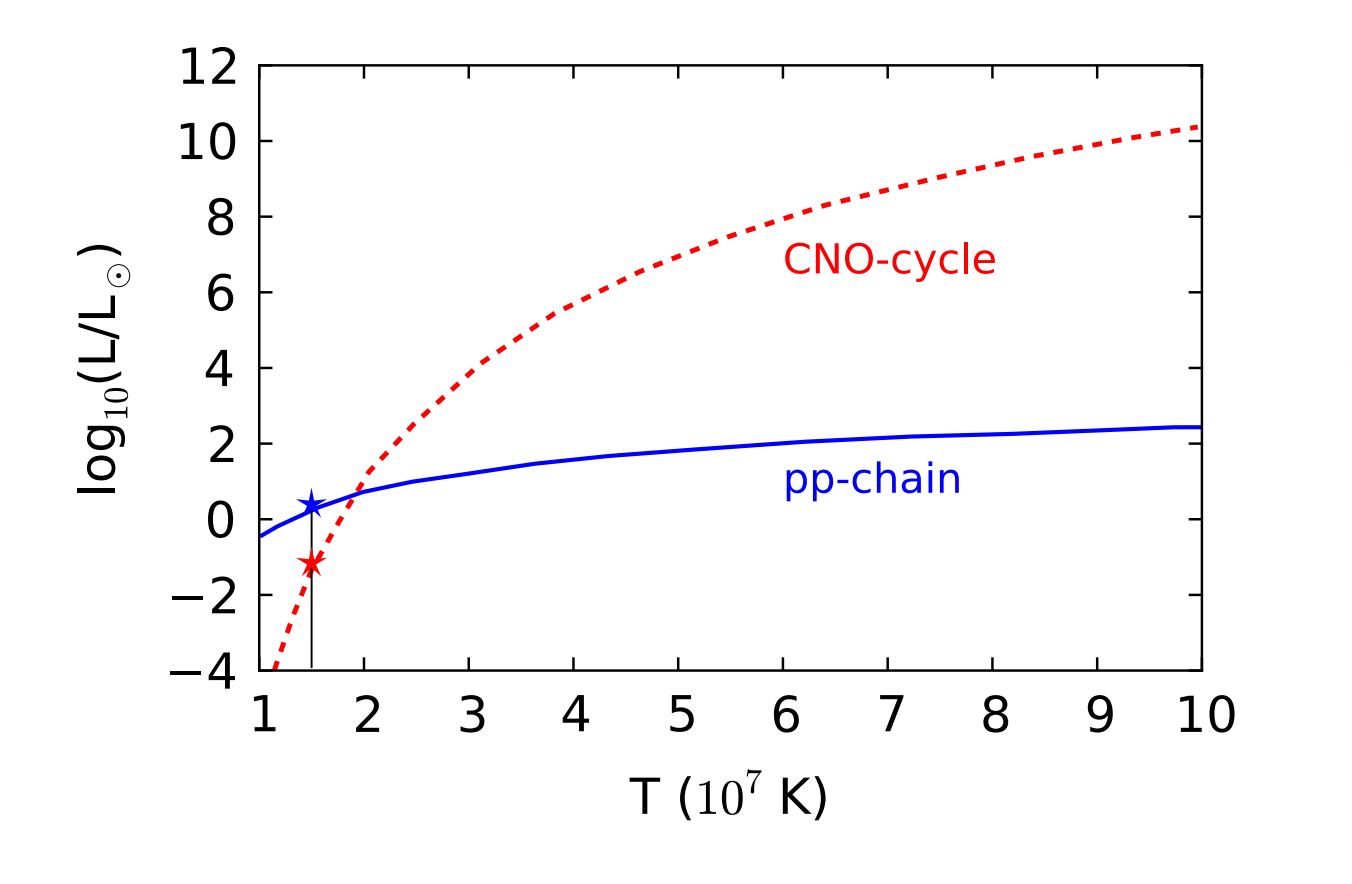
\includegraphics[width=\linewidth]{figures/energyProduction.png}
\label{fig: setup}
\caption{Depiction of the experimental setup used in this work, including the angled target holder, HPGe detector, and cold trap.}
\end{figure}



\subsection{Radiation detection}
\label{sec: detectors}

Generally speaking, the first step in the design of an experiment is understanding the necessary detection system to match the reaction. This is because, like a child trying to reconstruct a broken Lego set, measurements are done by measuring the products of a reaction and trying to work backwards to understand its form and function. In nuclear physics experiments, there are three primary classes of radiation to consider as the reaction products: 1) energetic charged particles, 2) neutrons, and 3) electromagnetic radiation (photons). Of these, the first class can be further subdivided into heavy ions, like the proton, $\alpha$ particle, or other nuclei, versus light particles, namely electrons. For all classifications of particles, they are detected primarily through energy deposition into another medium, with the specific interaction dependent on the type of particle. These methods will be introduced below, but the reader is referred to cite{KnollBook} for a complete discussion of radiation interaction with matter and subsequent detection techniques.  

For example, for charged particles in class 1, the dominant mechanism for energy deposition is through collisions with atomic electrons mediated by the electromagnetic force. As the particles pass through a medium, it generates an electromagnetic field in the surrounding space, which induces excitation in atomic electrons and even ionization if the energy is large enough. Each such interaction results in energy transfer from the incident particle to its neighborhood, slowing it to an eventual stop (usually). In many cases, the particle will stop inside the material, meaning that all of the energy was deposited. On the other hand, it is possible for the particle to pass outside of the medium due to its trajectory, meaning that only a fraction of the total energy from the particle will be deposited in the material. The path a particle traces through a medium is dependent primarily on its own properties, like mass, as heavier particles are more resistant to changes in momentum from interactions with atomic electrons, while an electron's path in a medium is typically chaotic, with significant scattering from interactions with other electrons. The detection medium thus plays little part in the detection of charged radiation.

Neutrons, by contrast, interact significantly differently with matter because of their electrically neutral state. Because they cannot react via the electromagnetic interaction, they can only exchange energy with their surrounding through the strong nuclear interaction. This implies that they will only have meaningful interactions with atomic nuclei inside of the detection material. This presents a significant challenge, however, as atomic nuclei occupy only a minuscule volume of space. This makes the medium in which the neutrons are detected much more important. In order to increase the probability of detection, the medium would ideally have a higher density, increasing the number of potential interaction sites for the neutron. Unfortunately, this can introduce another problem, as higher density materials are often those with higher mass nuclei as constituents. While such material will have a greater chance to interact with the incident neutrons, these heavy nuclei will not acquire significant energy in collisions due to conservation of energy and momentum, similar to how the momentum of heavy charged particles is largely unaffected by interactions with atomic electrons. As such, a neutron traveling in a high-density material with heavy nuclei may bounce chaotically many times before exiting the medium without depositing enough energy to produce a strong enough signal to be detected by the system's electronics. Therefore, in the detection of neutrons, the medium is almost always chosen to be composed of light elements, which are more favorable for the detection of neutrons as each collision will produce a more significant exchange of energy with the medium. Materials with a high neutron cross section, like boron on $\ce{^{3}He}$, are typically chosen as detection media. Due to the challenges of detecting high-energy (several MeV or greater) neutrons, a common technique for experiments involving neutrons is time-of-flight. In these cases, it is extremely unlikely to capture all of the neutron energy in a detection medium, so by measuring the time between neutron emission and interaction in a detector at a known distance the velocity, and kinetic energy, of the neutron is determined. This, however, necessitates a detailed understanding of the timing characteristics of a detector medium.

Finally, for quanta of electromagnetic radiation, or photons the interaction proceeds through yet different means. As an electrically neutral particle, photons do not interact with the medium in general and only at discrete points through the atomic electrons. As such, the interactions are much more probable than those of the neutron while being less than those of charged particles. Similar to charged particles, though, it is highly likely that photon interactions with matter result in a much higher chance to deposit all of the photon's energy in the medium. Clearly, by increasing the elemental number of the detection material's constituents, the probability of interaction with photons increases by increasing the number of possible interaction sites. As such, higher $Z$ materials are preferred for the detection of photons. 

On balance, there are three primary modes for photons to interact with matter: 1) the photoelectric effect, 2) Compton scattering, and 3) electron-positron pair production cite{KnollBook}. Fig. \ref{fig: radiationInteraction} illustrates these possible interactions and Fig. \ref{fig: gammaSpec} depicts the ways in which these effects manifest in measured spectra. 


\begin{figure}
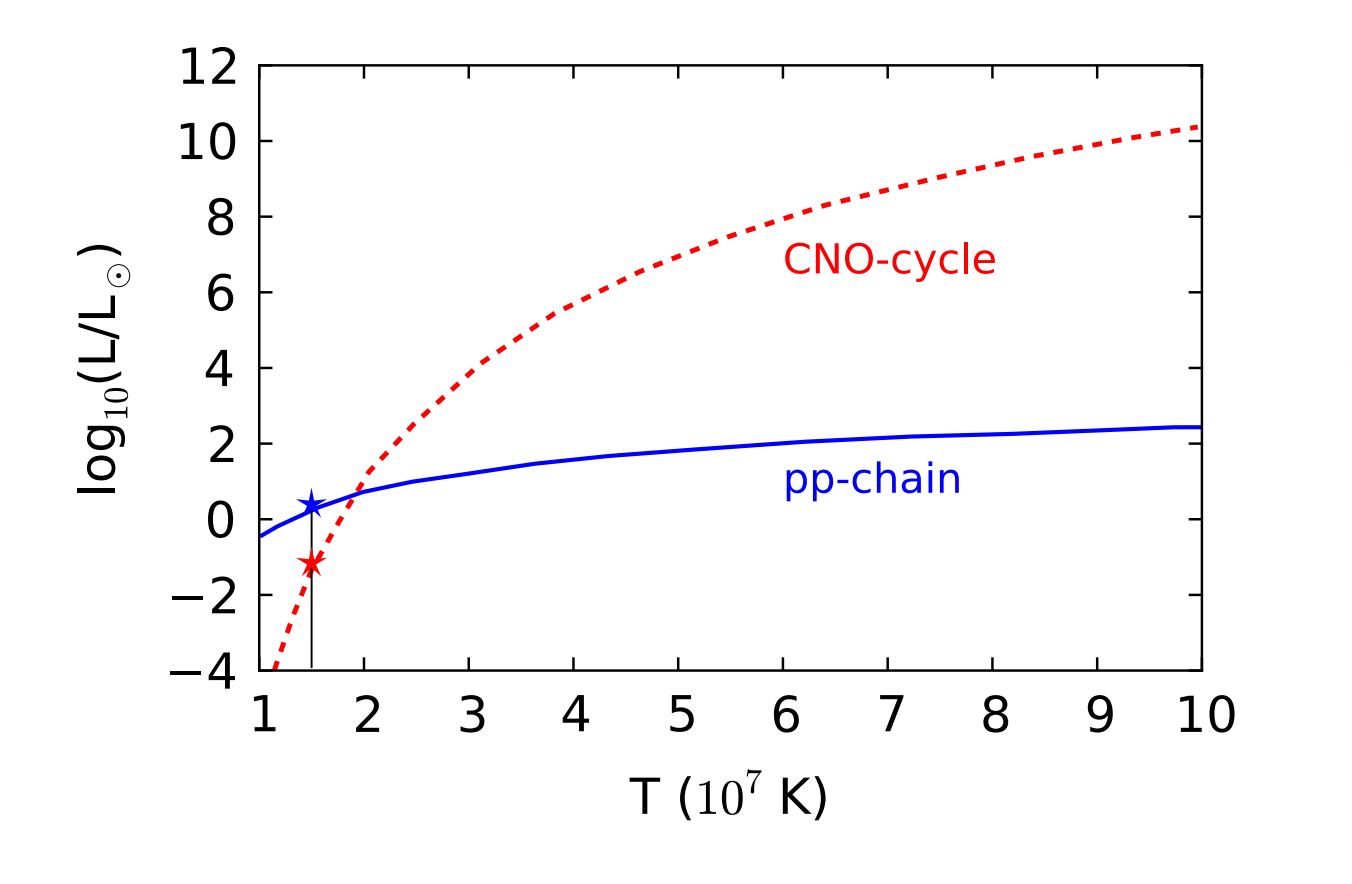
\includegraphics[width=\linewidth]{figures/energyProduction.png}
\label{fig: radiationInteraction}
\caption{Depiction of the modes for photons to interact with matter, showing a) the photoelectric effect, b) Compton scattering, and c) electron-positron pair production. }
\end{figure}


In photoelectric absorption, the photon transfers its energy to an atomic electron, leaving it in an excited state or ionizing it completely, where the electron deposits its energy like any other charged particle. If ejected, the electron will have energy $E_{e}$:

\begin{equation}
E_{e} = E_{\gamma} - E_{b}
\end{equation} 

\noindent where $E_{\gamma}$ is the incident photon energy and $E_{b}$ is the binding energy of the electron. In these cases, the electron is most likely ejected from the innermost atomic shell. For low-energy photons (below $\sim$1 MeV), this is the dominant interaction process cite{KnollBook}. 

Compton scattering is a similar process in that it also ends up producing an energetic electron inside the detection medium. In this type of interaction, a photon scatters inelastically from an atomic electron, imparting some of its energy to the electron and changing the momentum of both. Unlike the photoelectric effect, not all of the photon's energy is absorbed by the electron. As such, any of the interactions can occur again in the medium, like subsequent scatterings, full photoelectric absorption, or pair production, or the scattered photon could leave the material entirely. For the former conditions, the full energy of the photon will still (likely) be absorbed in the material. However, in the event that a subsequent scattered photon leaves a detection medium, this will manifest in the total energy measured in this event being lower than the true incident photon energy, artificially reducing the true signal and increasing the background. This is known as the Compton edge, which is shown in Fig \ref{fig: gammaSpec}. This effect is also the dominant effect in cases where the phtoon has a middle range of energies (between $\sim$ 1 - 6 MeV) cite{KnollBook}.

The final mechanism by which photons interact with matter is through electron-positron pair production, often shortened to just pair production. This occurs when a photon traveling spontaneously transforms into a matter-antimatter pair, the electron and positron, respectively.  This effect is induced by an interaction with a virtual photon from the electromagnetic field in the space the real photon is traveling. For this to occur, the photon's energy must be greater than the rest mass-energy of the pair, namely 1.022 MeV for electron-positron. After creation, the pair will share the total original energy (less their rest mass-energy) and momentum of the photon in their subsequent kinetic energies and momenta. From this point, the electron will continue to scatter and deposit energy in the normal manner for charged particles, while the positron will annihilate with one of the atomic electrons in the surrounding material, creating to diametrically opposed gamma-rays at 511 keV. With these, there are three potential outcomes: 1) the two new photons will interact with the surrounding medium through the processes already detailed, depositing their energy, and resulting in the total deposition of the initial photon's energy in the detection medium; 2) one of the new 511 keV photons will leave the detector without interacting and result in a deposition of the total initial energy less 511 keV; 3) both of the subsequent 511 keV photons leave the detector, resulting in an energy deposition of the total initial photon's energy minus 1.022 MeV. The two situations where a subsequent photon leaves the material are more comon with higher initial photon energies, manifesting in their own peaks in a measured spectrum. These are called escape peaks, shown in Fig. \ref{fig: gammaSpec}, with the single escape peak being when one photon leaves the medium and the double arising when both 511 keV photons escape the system. Whereas the full deposition of the photons energy is also shown in that spectrun and known as the full-energy peak. 

\begin{figure}
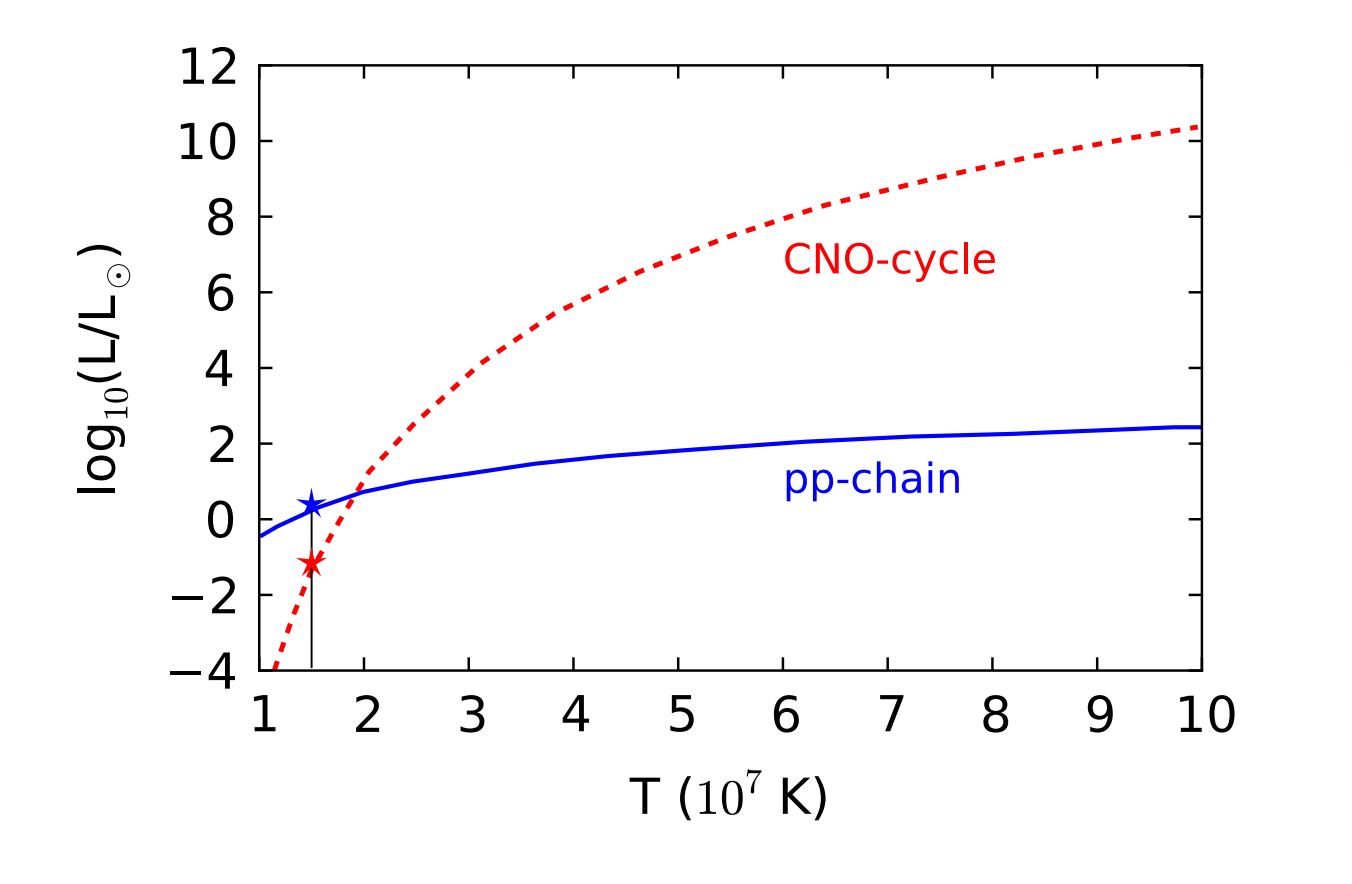
\includegraphics[width=\linewidth]{figures/energyProduction.png}
\label{fig: gammaSpec}
\caption{Cartoon depiction of an example experimental spectrum for photon interactions. Artifacts from the ways in which photons interact with matter are highlighted in the spectrum and are common in experimental gamma spectra  }
\end{figure}


This work is concerned ultimately with measuring photons as reaction products and employed high-purity germanium (HPGe) semiconducting detectors for that purpose. These are characterized by having a relatively small band gap between the electrons within the valence and conducting bands. When photons enter the Ge crystal, they excite electrons across the band gap from the valence to the conducting band, leaving behind vacancies, known as holes, in the valence band. These excited electron-hole pairs feel an electric field supplied by the detector's bias voltage, causing them to drift to the charge collection electrodes at the end of the crystal, resulting in an electric current pulse. Since HPGe has a small band gap, around 0.7 eV (depending on impurities) cite{KnollBook}, it requires constant cooling of the medium by liquid nitrogen in order to reduce the number of electron-hole pairs created by thermal excitations in the valence band. However, by cooling these detectors, HPGe becomes extremely useful because of the large number of charge carries produced by the small band gap in an energy deposition event, giving superior energy resolution. It is for this reason that HPGe detectors are ubiquitous in nuclear physics laboratories around the world - even those shown in movies. Comparatively though, HPGe detectors are more expensive and (typically) less efficient than NaI detectors, which are the other primary type of photon detector, so they are not which downsides to use as well. 

Thus, in every experiment it is important to anticipate reaction outcomes when planning what type of radiation detection system to employ. As stated, this work was concerned with the measurement of high-energy photons from a nuclear reaction, so we chose to use HPGe detectors for their superior resolution.




\section{Cross-section measurements}
\label{sec: cs experiment}

This set of data was taken over the course of five* separate experiments. The first occurred at the University of Notre Dame's Nuclear Science Laboratory (NSL) in January of 2018 and covered the proton energy range of E$_{p}$ = 800 - 1200 keV. The experiment was then continued at the Compact Accelerator System for Performing Nuclear Astrophysics (CASPAR) facility at the Sanford Underground Research Facility located in Lead, South Dakota in three increments: February 2018, May 2018, and August / September 2018. These measurements covered the energy range from E$_{p}$ = 270 - 1100 keV, in order to measure the $^{14}$N$\left( p,\gamma \right) ^{15}$O reaction cross-section to compare the performance of the CASPAR facility to an above-ground laboratory.


\subsection{Experiment at Notre Dame}
\label{sec: expND}

The goal of this experiment was to measure the $^{14}$N$\left( p,\gamma \right) ^{15}$O reaction cross-section in a low energy range of the Sta. Ana accelerator, proton energy range of E$_{p}$ = 800 - 1200 keV, to provide a self consistent data set with which to compare the results of a measurement at CASPAR and test experimental procedures before moving to the more challenging environment at CASPAR. The setup used in this experimental phase is depicted in Fig. \ref{fig: setup}. In order to reduce confounding effects, it was also used identically at CASPAR. 

In this measurement, the $\gamma$-rays were observed with a coaxial p-type HPGe detector rated with 130\% relative efficiency (relative to the efficiency of a 3" $\cross$ 3" NaI detector with 1332 keV $\gamma$-rays). Five mm of lead shielding was placed in front of the crystal's face to reduce the number of low-energy x-rays entering the detector (<100 keV photon energy) because they increase the dead time in the electronics decreasing processing time for signals of interest. The detector was placed at an angle of 55$^{\deg}$ in order to minimize any angular distribution effects on the cross section, as that is the minimum of the second order Legendre polynomial which describes the angular behavior of the cross section. The detector was placed on a sliding, isolating platform, enabling it's distance to the target to be easily changed. Measurements were primarily taken with the detector in close geometry, with only 2 mm between the target and lead shielding (closer would have resulted in them touching on the corner because of their different orientation) but some were measured in far geometry, up to 25.4 cm between the target and lead shielding. This was done to provide a reference for the effects of summing on our detector response at high energies, which will be discussed further in following chapter. Additionally, a more detailed description of all targets used in this work will be presented in the next chapter, but for completeness, this portion of the experiment utilized a solid, TiN target. 


\subsection{The CASPAR facility}
\label{sec: caspar}

In an attempt to extend the data range down to the lowest possible energies and provide a proof-of-principle for the facility, a second phase of the experiment was performed at the CASPAR facility. CASPAR is the Compact Accelerator System for Performing Astrophysical Research, located on the 4850 ft level of the Sanford Underground Research Facility, and is the first underground accelerator facility in the United States. This facility was originially the Homestake Gold Mine in Western South Dakota, just outside (and underneath) the town of Lead. It is also the location of the famous Ray Davis underground neutrino experiment in which the solar neutrino problem was identified cite{DavisExperiment}. The accelerator located at the facility is the recently refurbished JN Van de Graaff, which had been employed at the NSL since its arrival in the early 2000's. Fig. \ref{fig: casparPictures} shows some pictures of the facility.


\begin{figure}
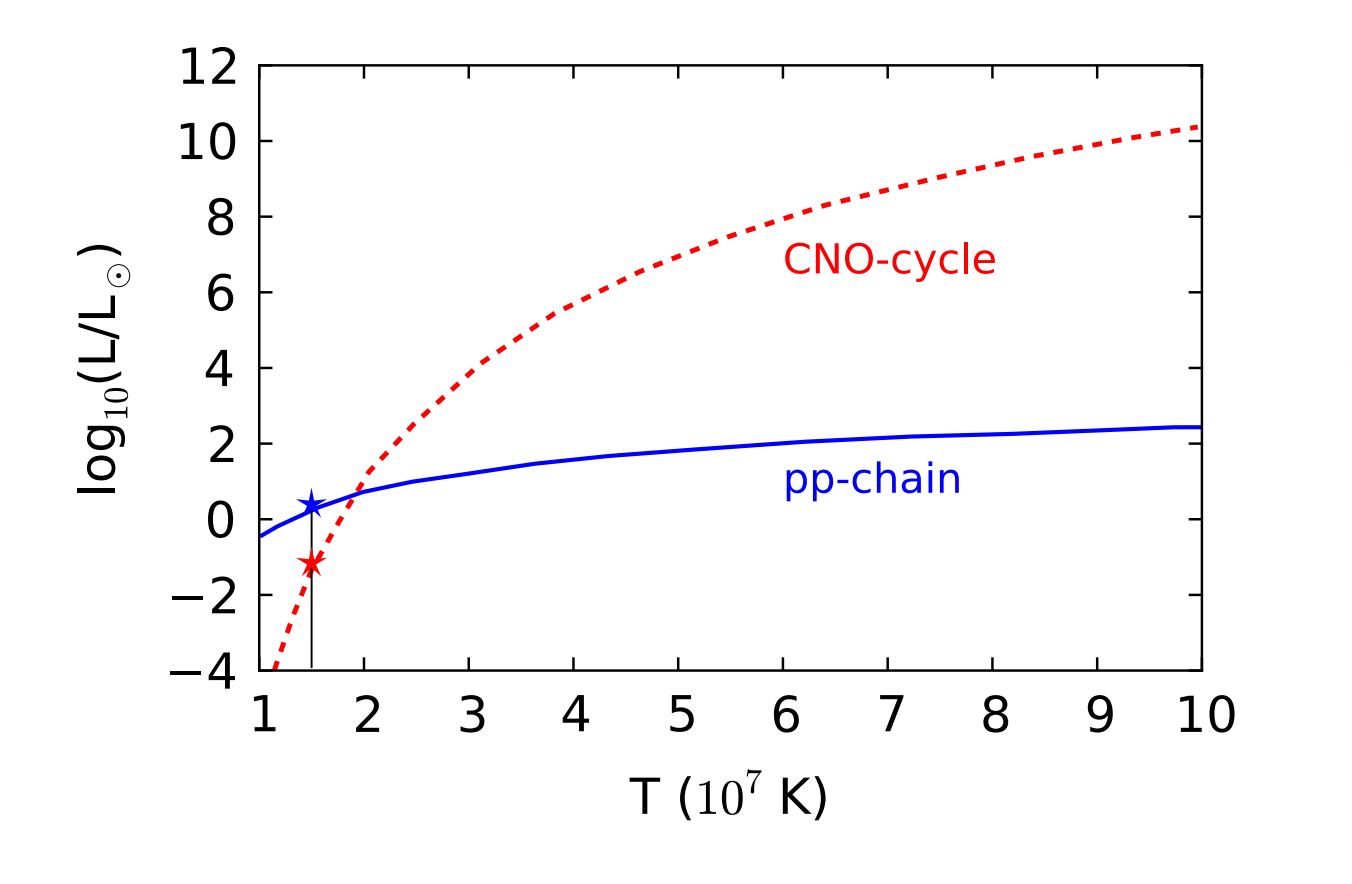
\includegraphics[width=\linewidth]{figures/energyProduction.png}
\label{fig: casparPictures}
\caption{Pictures of the CASPAR facility. }
\end{figure}



Some of the problems with performing low-energy nuclear astrophysics measurements were detailed in Section \ref{sec: thermonuclear reaction rates}. The most significant of these is the diminishing cross section at astrophysically relevant energies due to Coulomb repulsion. There are a number of techniques for mitigating this problem: 1) extrapolating from higher energy with techniques like $R$-matrix (see Section \ref{sec: r-matrix}), 2) increasing the reaction yield with high-intensity accelerators and targets, 3) performing long term measurements to enable measurements of ridiculously low cross section reactions, and 4) drastically reduce cosmic background to increase the signal to background ratio and prevent these events from hiding a signal of interest. Of these, CASPAR is equipped to employ the solutions of 2, 3, and 4. In Section \ref{sec: ion sources}, the RF ion source utilized inside the JN accelerator was described, but the useful feature is that it can deliver proton and $\alpha$ beams up to 150 $\mu A$, increasing the experimental yield dramatically. Additionally, without the constraints and competition of multiple running groups, which is the reality at larger labs like the NSL or the National Superconducting Cyclotron Laboratory at Michigan State University, the facility is able to measure a reaction as long as necessary (five weeks in this case). Finally, with nearly a mile of rock cover above the facility provided by the mountains, the facility has excellent passive shielding. The background reduction compared to a surface laboratory like the NSL is shown in Fig. \ref{fig: backgroundComparison}. Strictly speaking, due to the high content of the uranium and thorium decay chains in the surrounding rock, the radiogenic background (that at energies below $\sim$2.6 MeV) is actually higher at the CASPAR facility than the surface. This, however, can be (and is) addressed by adding additional lead shielding around the detector crystal. Taken together, these features advance CASPAR beyond the capabilities of other laboratories performing nuclear astrophysics experiments and make it particularly useful. It's for these reasons that it was chosen to perform the low-energy phase of this work. 


\begin{figure}
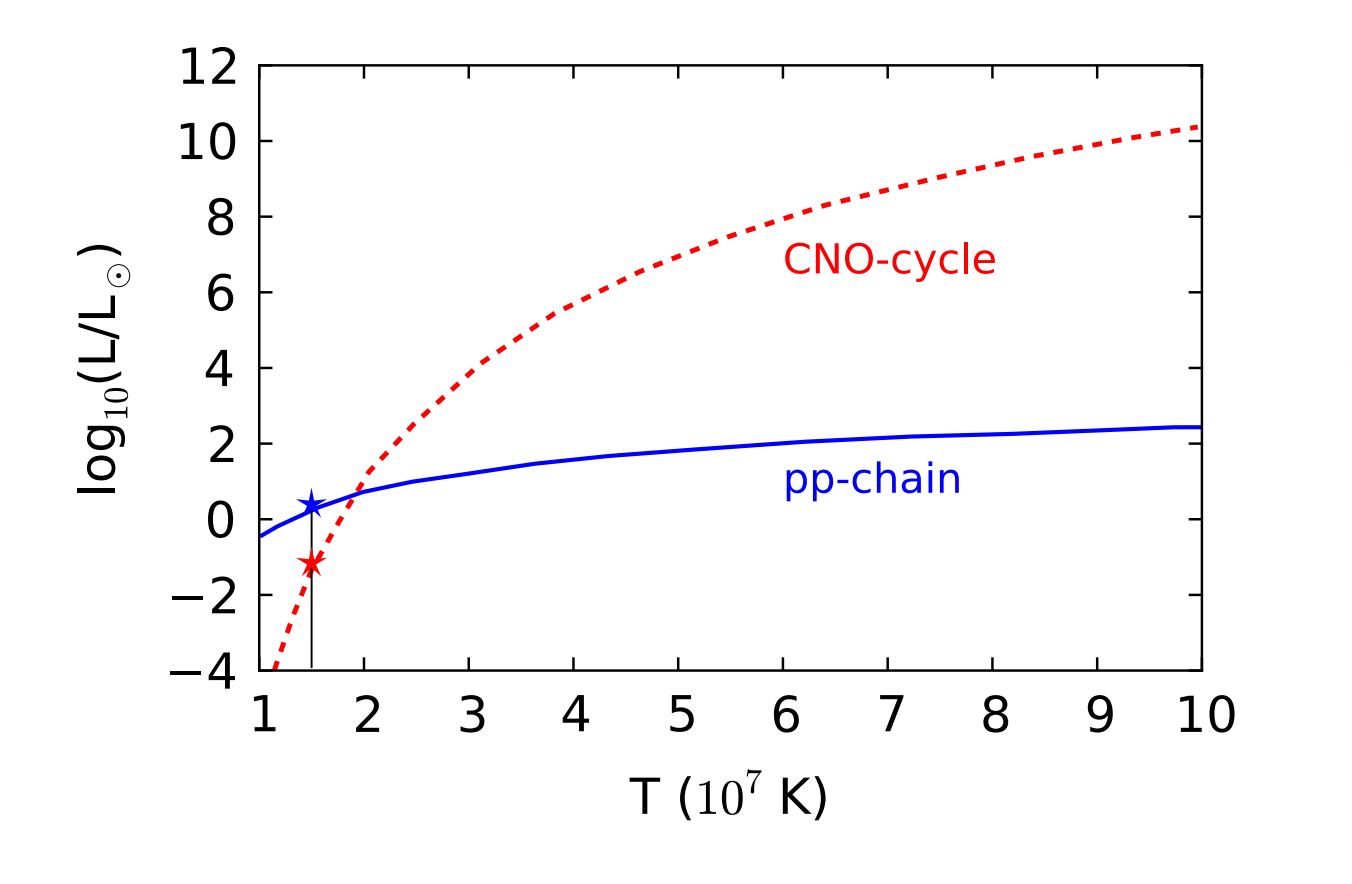
\includegraphics[width=\linewidth]{figures/energyProduction.png}
\label{fig: backgroundComparison}
\caption{Background $\gamma$ spectrum taken at the NSL, CASPAR, and CASPAR utilizing passive lead shielding, with a) showing the full spectrum and b) showing a subset of the spectrum at low energies to highlight the radiogenic background, which is higher at CASPAR without lead shielding. Clearly, the facility provides a prodigious reduction of cosmogenic background, making the facility advantageous for low-energy nuclear astrophysics experiments.}
\end{figure}

Additionally, the JN accelerator at CASPAR expands on the potential measurement range compared to the LUNA II facility, the other preeminent underground nuclear astrophysics laboratory in the world cite{Formicola2005}. The two have similar background reduction due to their environments and equal capacity to perform extensive measurements. However, until the LUNA MV facility is completed cite{something}, CASPAR's expanded energy regime allows its measurements to overlap with those performed at surface laboratories, unlike LUNA II, making it the ideal facility for low-energy nuclear astrophysics. 

The measurements at CASPAR were undertaken over the course of five weeks in February 2018, May 2018, and August / September 2018. These covered the proton energy range from E$_{p}$ = 270 - 1100 keV, overlapping with the measurements at the NSL. As stated in Section \ref{sec: expND}, the equipment like detector, electronics, and overall setup used in this campaign was the same as what was used at the NSL. The only significant different was the different targets used in this experiment. These were sputtered ZrN targets of varying thickness (\textbf{TARGET THICKNESSES}) produced specifically for this experiment in Bochum, Germany. Given the high intensity of the beam delivered at CASPAR, these were constantly monitored for degredation and carbon buildup to reduce target effects on the measurement. 





\section{Lifetime measurement}
\label{sec: lifetime experiment}

\subsection{The Doppler-Shift Attsenuation Method for lifetime measurements}
\label{sec: DSAM}


Nuclear lifetimes are important observables to measure because they provide a link to understanding the strong nuclear force. They are necessary to determine the reduced transition probabilities which are one of the most important probes of nuclear structure and the forces governing the behavior of nuclei.The Doppler Shift Attenuation Method (DSAM) is a well characterized method for determining the lifetimes of excited nuclear states that decay via gamma emission in the range of 10$^{-11}$ - 10$^{-15}$ s \cite{Blaugrund1966}. The ranges where DSAM is applicable are compared with other common methods for determining nuclear lifetimes in Fig. \ref{fig: lifetimeRanges}. 


\begin{figure}
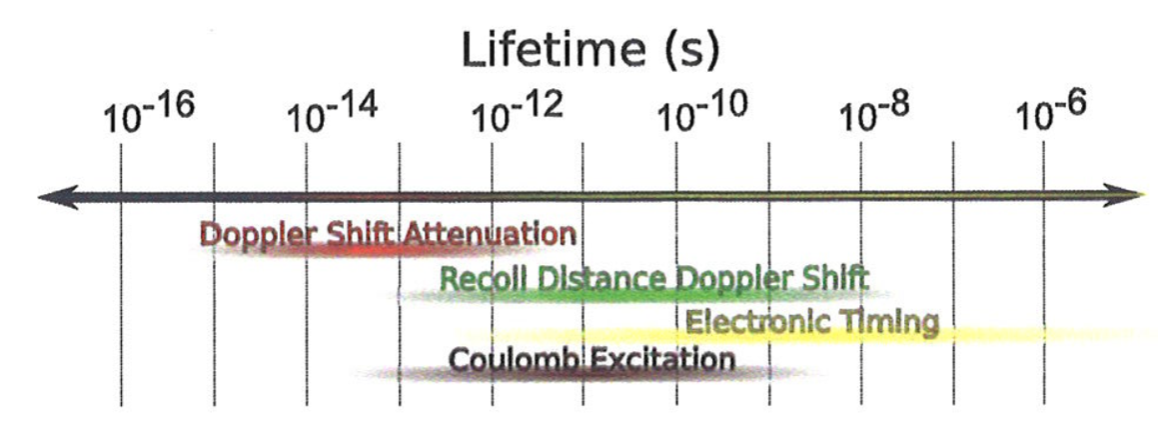
\includegraphics[width=\linewidth]{figures/lifetimeTechniques.png}
\label{fig: lifetimeRanges}
\caption{Ranges over which the different lifetime measuring techniques are valid (Obtained via personal communication with M.K. Smith in 2017). \textbf{CHANGE THIS REFERENCE}}
\end{figure}


The basic idea of DSAM is to produce an excited nucleus inside of a dense target in which the reaction product will decay. The de-excitation of the nucleus then takes place either while the nucleus is slowing down or after it stops, depending on the lifetime of the specific state and the stopping within the target. Then, as is true with the classical Doppler shift, the energy of the emitted $\gamma$-rays are shifted depending on their emission angle relative to the motion of their source, the decaying nucleus. Thus, $\gamma$'s emitted at different velocities during the slow-down and detected at given angles will have a spread of energies. Specifically, for a given nucleus decaying at a time $t$ with a speed of $v(t)$, the Doppler shifted energy of the gamma ray, $E_{\gamma}$, is 

\begin{equation}
E_{\gamma} = E_{0} \left(1 + \dfrac{v(t)}{c} \cos (\theta)   \right),
\label{eqn: doppler1}
\end{equation}

\noindent where $E_{0}$ is the energy of the decay for a nucleus at rest, $c$ is the speed of light, and $\theta$ is the lab angle between the momentum vectors of the decaying nucleus and gamma ray, respectively. A depiction of this scenario is given in Fig. \ref{fig: decay}.

\begin{figure}
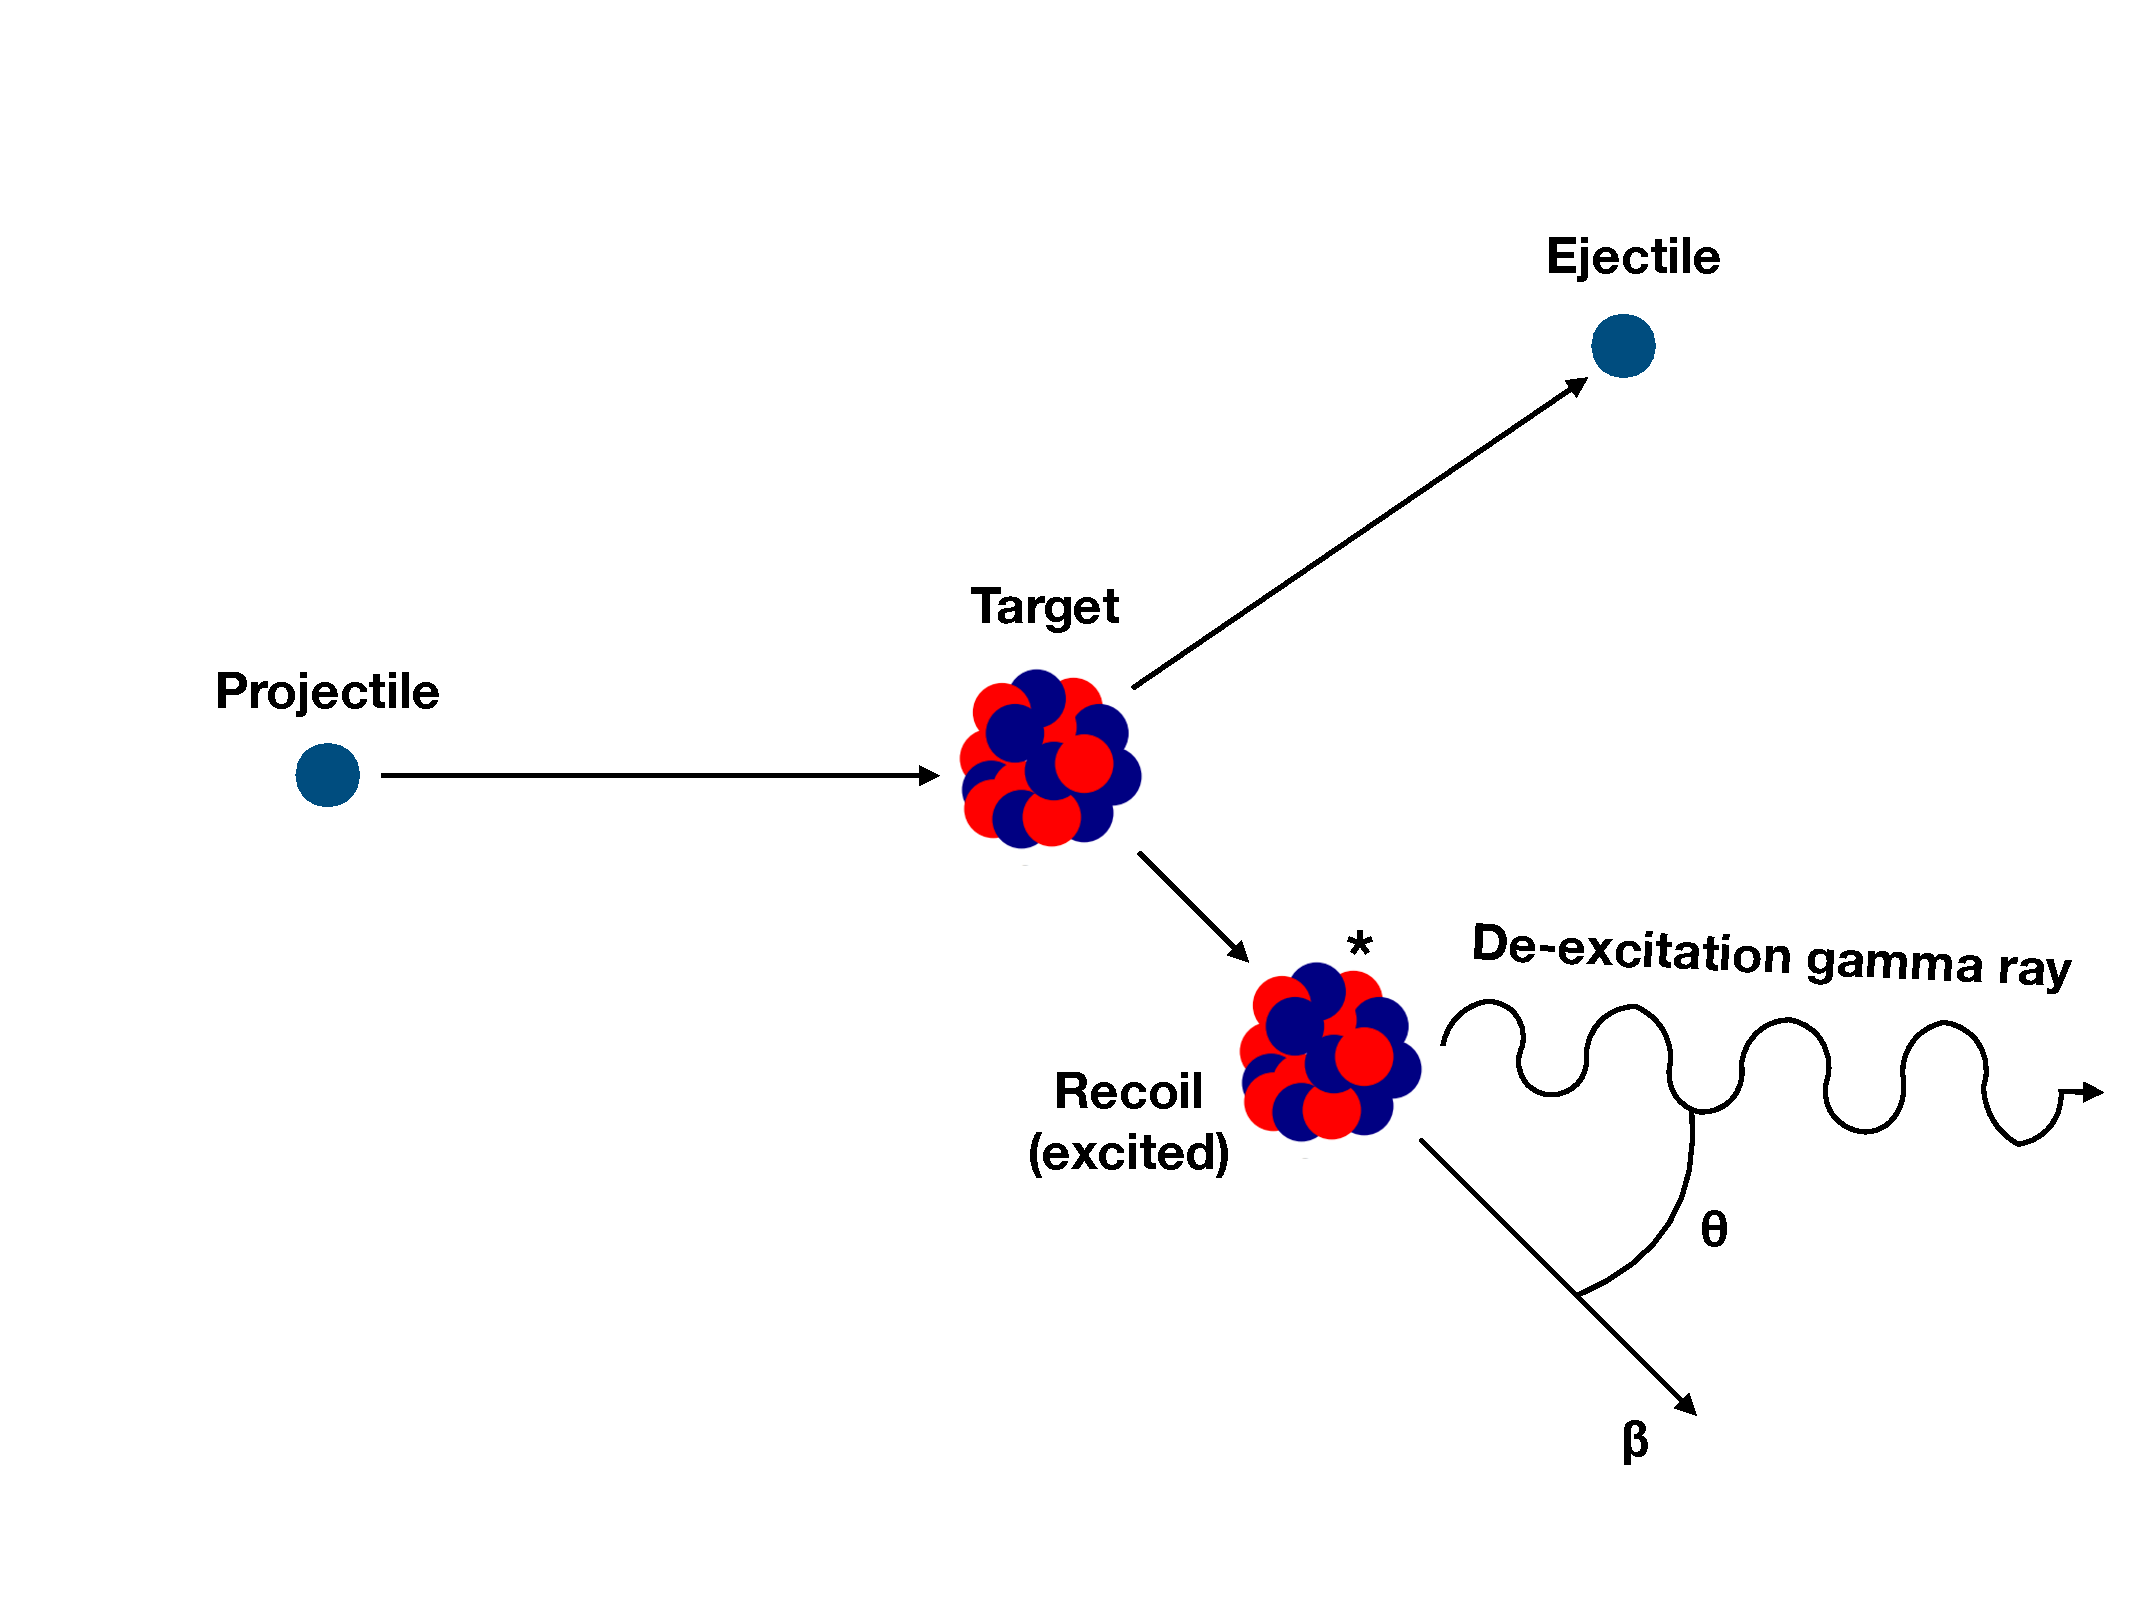
\includegraphics[width=\linewidth]{figures/decay.pdf}
\label{fig: decay}
\caption{A generic nuclear reaction showing the creation of an excited nucleus and subsequent decay, causing a Doppler shift in the measured energy of the $\gamma$ ray.}
\end{figure}


As the nuclear decay process is statistical in nature, the measured spectrum of gamma energies for a particular transition is a continuous distribution of energies from the unshifted, rest energy peak to the maximally Doppler shifted peak. As Equation \ref{eqn: doppler1} was specific to a single transition, it is necessary to consider the entire sample of decays measured. By defining the average velocity of all nuclei at the time of decay, $\overline{v}$, the initial velocity of all recoiling nuclei, $v_{0}$, and their ratio, $F(\tau)$, called the attenuation factor, it is possible to relate the behavior of the entire distribution to the lifetime of the state. This is 

\begin{equation}
E_{\gamma} = E_{0} \left(1 + F(\tau) \beta_{0} \cos (\theta)   \right),
\label{eqn: dopplerFull}
\end{equation}

\noindent where $\beta_{0} = v_{0}/c$ is the relativistic velocity factor. $F(\tau)$ therefore provides an analytical relation between the nuclear lifetime and the measured Doppler shift, given by Blaugrund in 1966 \cite{Blaugrund1966} as

\begin{equation}
F(\tau) \beta_{0} = \dfrac{1}{\tau} \int_{0}^{\infty} \beta(t) \exp \left( \dfrac{t}{\tau} \right) dt,
\end{equation} 

\noindent where $\beta(t) = v(t)/c$ is the time dependent relativistic velocity factor. The devil, however, is in the details of calculating $\beta(t)$, since it is reliant on stopping powers of the nuclei in the target material, implying an accurate knowledge of the target composition and population pattern of the nucleus. In some cases the feeding is not well known and for nearly all cases, there is an estimated uncertainty in the assessment of stopping powers of materials to be at least 10\%.

It is important to note that the Doppler shift can either increase or decrease the energy of the measured $\gamma$ ray, depending on whether the emitted gamma ray is at forward or backward angles relative to the nucleus' motion. Fig. \ref{fig: dopplerShift} shows the Doppler effect on a measured $\gamma$ spectrum, shifting the energy according to the measured angle. It is evident that the lifetime of a particular excited state has a dramatic effect on the location and shape of this distribution, for the longer a specific lifetime is, the broader its measured distribution will be (and vice versa) while the shift in the centroid of the peak will be lower than that of short lifetimes where the nucleus has a relatively higher velocity upon decay. 

\begin{figure}
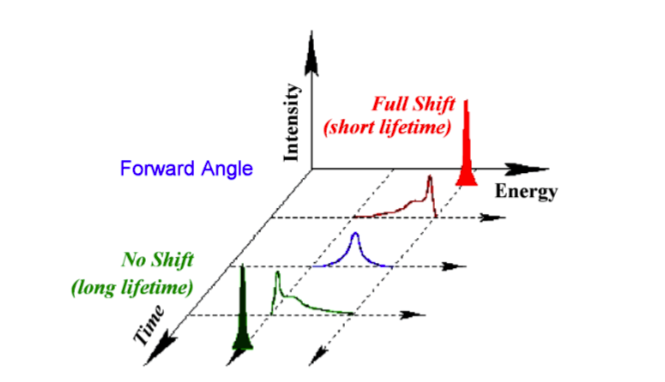
\includegraphics[width=\linewidth]{figures/dopplerEffects.png}
\label{fig: dopplerShift}
\caption{The effect of the nuclear lifetime on the measured gamma spectrum for a given experimental scenario \cite{Schimpf2011}. In forward angles, the $\gamma$'s energy is shifted to higher values, while the the measured energy of the $\gamma$ is lower at backward angles, with the maximum shift in either direction coming when the $\gamma$ is emitted in a direction parallel to the motion of the decaying nucleus. A $\gamma$ emitted at $90^{\deg}$ is unshifted and unbroadened. }
\end{figure}

Therefore, by performing a lineshape analysis on the distribution of the measured $\gamma$'s and a mapping of the distribution's shift with angle one can determine the nuclear lifetime. The procedure for the Doppler shift determination is particularly straightforward. By plotting the resulting centroids measured for the gamma distribution vs the $\cos(\theta)$, one should obtain a straight line, the slope of which is the product $E_{0} \beta_{0} F(\tau)$. So, for a given experimental approach with the same reaction and targets, this slope and therefore attenuation factor should match. This was not the case for the Bertone \textit{et al.} and Sch{\"u}rmann \textit{et al.} works \cite{Bertone2001, Schurmann2008}, where the authors used the same reaction on ostensibly the same targets and reached incongruous $F(\tau)$ values. 
 

\subsection{Target production}
\label{sec: implantation}


Why Implantation
Seuthe
How did we produce them and why


\subsection{Measurement at Notre Dame}
\label{sec: lifetimeND}


How did we do it
Highlight similarities and differences to previous measurements.




% % uncomment the following lines,
% if using chapter-wise bibliography
%
% \bibliographystyle{ndnatbib}
% \bibliography{example}


%
% Chapter 3
%

%
% Modified by Megan Patnott
% Last Change: Jan 18, 2013
%
%%%%%%%%%%%%%%%%%%%%%%%%%%%%%%%%%%%%%%%%%%%%%%%%%%%%%%%%%%%%%%%%%%%%%%%%
%
% Modified by Bryce Frentz
% Last Change: 2018
%
%%%%%%%%%%%%%%%%%%%%%%%%%%%%%%%%%%%%%%%%%%%%%%%%%%%%%%%%%%%%%%%%%%%%%%%%
%
% Sample Notre Dame Thesis/Dissertation
% Using Donald Peterson's ndthesis classfile
%
% Written by Jeff Squyres and Don Peterson
%
% Provided by the Information Technology Committee of
%   the Graduate Student Union
%   http://www.gsu.nd.edu/
%
% Nothing in this document is serious except the format.  :-)
%
% If you have any suggestions, comments, questions, please send e-mail
% to: ndthesis@gsu.nd.edu
%
%%%%%%%%%%%%%%%%%%%%%%%%%%%%%%%%%%%%%%%%%%%%%%%%%%%%%%%%%%%%%%%%%%%%%%%%

%
% Chapter 3
%

\chapter{Cross section data reduction and analysis}
\label{chap: data}

\section{Introduction}

In aggregate, the data taken at both the CASPAR and NSL experiments consists of $\gamma$-ray energy data from the $^{14}$N$\left( p,\gamma \right) ^{15}$O reaction, observed with a single, 130\% HPGe detector placed at $55^{\degree}$ relative to the beam direction. These data were collected for reactions over the combined proton energy range of 270 - 1200 keV. The primary interest of these experiments was monitoring the R/DC$\rightarrow$GS transition and the R/DC$\rightarrow$6.79 MeV + 6.79 MeV$\rightarrow$GS transition sequence. As such, the energies of the concerned photons ranged in energy from $\sim$600 keV up to $\sim$8500 keV. This chapter details the processes by which this data is gathered and turned into an experimental cross section.

\section{Angular corrections}
\label{sec: angularCorrections}

The angular distribution of a cross section, $W$, can be described by

\begin{equation}
W_{\text{exp}} = a_{0} \left(1 + \sum_{i = 1}^{n} a_{i} Q_{i} P_{i} ( \cos (\theta) )    \right)
\end{equation}

\noindent where $a_{i}$ are the angular distribution coefficients, $Q_{i}$ are correction factors due to the finite size of a given detector, and the $P_{i} ( \cos (\theta) )$ are the Legendre polynomials of order $i$. For the conditions of this work, odd numbered terms as well as those of order higher than 2 give negligible contribution to the angular distribution. Therefore, the resulting angular distribution of this reaction is of the form

\begin{equation}
W_{\text{exp}} = a_{0} + a_{2} Q_{2} P_{2} ( \cos (\theta) ).
\end{equation}

Experimentally, to address any effects arising from an angular distribution of this form, the detector was placed at $55^{\degree}$. This is the zero of the 2nd order Legendre polynomial, thereby minimizing any effects on the cross section arising from the detector's angle. Simultaneously, this means that no correction of the data is necessary.


\section{Energy calibration}
\label{sec: energy calibration}

Detectors are calibrated with $\gamma$-rays of well-known energy from room background, given radioactive sources, like $^{137}$Cs or $^{60}$Co, and well-studied nuclear reactions, like $^{27}$Al($p, \gamma$)$^{28}$Si. The reactions are utilized in concert with the radioactive sources because no natural sources of radioactivity provide $\gamma$'s with energy higher than 3.6 MeV, whereas the $^{27}$Al($p, \gamma$)$^{28}$Si reaction provides $\gamma$ ray energies up to 10.7 MeV, ensuring that the detector is well calibrated over the entire energy range for $\gamma$'s that will be seen in the $^{14}$N$\left( p,\gamma \right) ^{15}$O reaction. The exact relationship between the the channel number in the acquisition system analog-to-digital converter (ADC) and the incident photon energy, $E_{\gamma}$, is characterized by the standard linear relationship

\begin{equation}
E_{\gamma} = m \times \text{Channel} + b
\end{equation}

\noindent where $m$ is simply the slope and $b$ the offset of the fit. For a HPGe detector, a linear relationship is sufficient and appropriate to describe the ADC response. However, this process was redone for every phase of the experiment because slightly different gains applied to the ADC's and signal amplifiers provide a different relationship in the electronics. Therefore, despite using the same detector, each phase of the experiment required its own energy calibration, an example of which is shown in Fig.\ \ref{fig: energyCalibration} for the CASPAR setup.


\begin{figure}
\centering
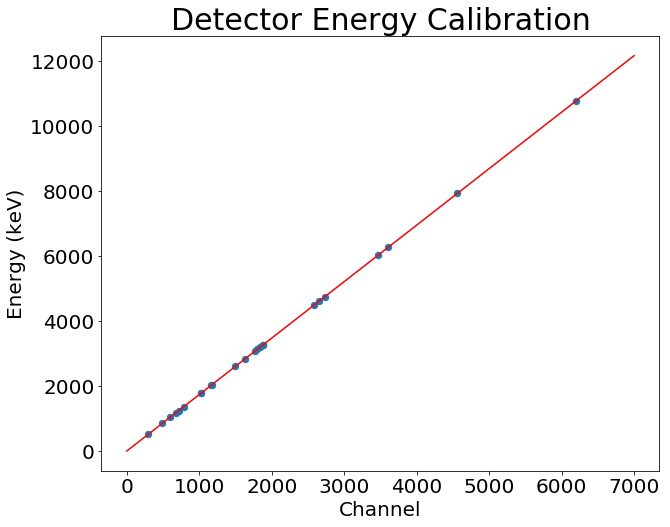
\includegraphics[width=0.8\linewidth]{figures/detEnergyCalibration.png}
\caption{Energy calibration curve for the HPGe detector taken at CASPAR. The calibration incorporated natural background, radioactive sources, and the products from the $^{27}$Al($p, \gamma$)$^{28}$Si reaction. }
\label{fig: energyCalibration}
\end{figure}





\section{Efficiency}
\label{sec: efficiency}

Efficiency is a term that can, in different contexts, have many different meanings. However, in experimental physics it is known to be the ratio for the response of an instrument to the actual physical quantity for which it is employed to measure. In these cases, it is the ratio between the photons recorded and those emitted in a given event. For this experiment, both the total efficiency, $\eta^{TOT}$, and the full-energy peak (FEP) efficiency, $\eta^{fep}$, were required. The total efficiency is the probability that the $\gamma$ ray enters and deposits any amount of energy within the detector, while, on the other hand, the FEP efficiency is the probability that the full energy of an emitted $\gamma$ ray will be deposited within the detector. As both efficiency types are dependent on the physical geometry of the system, they are determined for each experimental setup in turn. 

\subsection{Total efficiency}
\label{subsec: totEff}

The total efficiency of a detector / source geometry is the probability that a given photon from the source will enter and deposit any amount of energy within the detector. For extremely simple geometries, the total efficiency can be calculated following the approach laid out in Debertin and Helmer \cite{DebertinHelmerBook},

\begin{equation}
\eta^{TOT} = \dfrac{1}{4\pi} \int \left(1 - e^{-\mu x} \right) d\Omega
\end{equation}

\noindent where $\mu$ is the energy and absorber dependent attenuation coefficient, x is the position from the detector face, and the integration takes place over the solid angle of the detector from the front to the back. This formulation makes it abundantly clear that $\eta^{TOT}$ is so highly dependent on the geometry of the setup. 

However, in practice, there is no analytic formulation of the total efficiency because one needs to account for any potential scattering of $\gamma$-rays off of any surrounding material, like the shielding or target chamber, for example. Additionally, when measuring the total efficiency for a given setup, the presence of multiple decays from physical sources provides additional complications.

So, one can use the summing-out correction effects within one's data to determine the total efficiency of the detector. For each line in a spectrum, a ratio of the intensities in close and far geometries can be obtained, $R_{i} = I_{\gamma}^{close} / I_{\gamma}^{far}$, where $I$ is the measured intensity of the $\gamma$-ray. Further discussion on this point will follow in Sec. \ref{sec: summing}, but ultimately, this ratio can be used to determine the total efficiency. For transitions with summing present, this ratio is deflated by a factor because of the lost counts in the relevant peaks. Mathematically, this is expressed as

\begin{equation}
I_{\gamma}^{close} = R_{true} C_{out} I_{\gamma}^{far} = R_{true} (1-\eta^{tot}) I_{\gamma}^{far}
\end{equation}

\noindent where $R_{true}$ is the true, geometric difference between the near and far data without summing effects, $C_{out}-(1-\eta^{TOT})$ is the summing-out effect, and $eta^{TOT}$ is the total efficiency. For our data, the $R_{true}$ ratio was obtained by measuring the monoenergetic, isotropic decay from $^{12}$C($p, \gamma$)$^{13}$N reaction at 2365 keV. Thus, the $i$th transition's near/far ratio in the nitrogen data (which would contain summing effects) would allow us to determine the total efficiency by 

\begin{equation}
 I_{\gamma}^{close} = R_{i} I_{\gamma}^{far}
\end{equation}

\begin{equation}
R_{i} I_{\gamma}^{far} = R_{true} (1-\eta^{TOT}) I_{\gamma}^{far}
\end{equation}

\begin{equation}
\Rightarrow (1-\eta^{TOT}) = \dfrac{R_{i}}{R_{true}}.
\end{equation}


% Therefore, most commonly the total efficiency is determined using single-line radioactive sources, like $^{137}$Cs, with well known activity. In this case, when accounting for the ever-present background, the total efficiency is the total number of counts in a spectrum divided by the total number of decays occurring during the measurement time, which can be easily calculated with the radioactive decay law

%\begin{equation}
%N(t) = N_{0} e^{- \lambda t} \hfill A(t) = A_{0} e^{- \lambda t},
%\end{equation}

%\noindent where $N(t)$ is the number of nuclei remaining after time $t$, $N_{0}$ is the initial number of radioactive nuclei, $\lambda$ is the radioactive decay constant for a given nucleus, $A(t)$ is the activity of the source at time $t$ compared to the activity at time $t=0$ of $A_{0}$. The decay constant, $\lambda$, can be calculated from either the nuclear lifetime, $\tau$, or the decay half-life, $t_{1/2}$, as

%\begin{equation}
%\lambda = \dfrac{1}{\tau} \hfill \lambda = \dfrac{\text{ln}(2)}{t_{1/2}}.
%\end{equation}

%\noindent This is how the total efficiency for the detector systems was determined at 662 keV, the $\gamma$ energy from the decay of $^{137}$Cs.



\begin{figure}
\centering
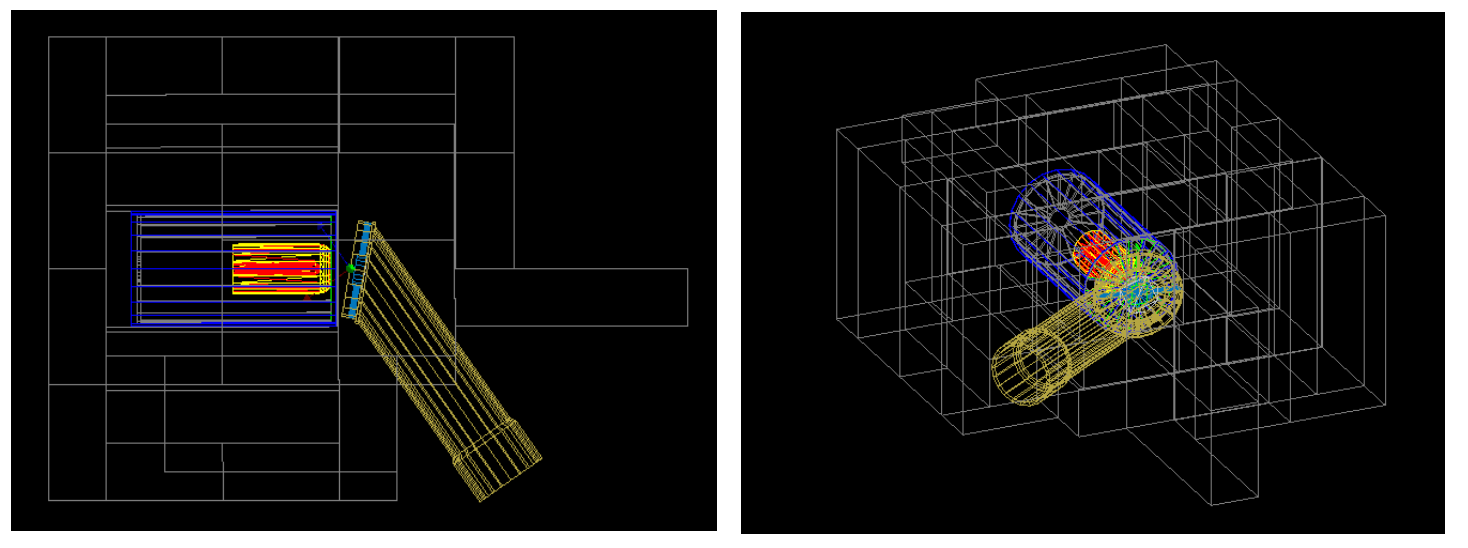
\includegraphics[width=\linewidth]{figures/shieldingSimulation.png}
\caption{Simulation of the experimental setup at CASPAR, including the target chamber (in gold), water cooling (in light blue), HPGe detector (in dark blue), and lead bricks for shielding (in gray). Both pictures are of the same experimental setup from different angles to convey the layout. Simulating this setup is necessary to determine the total efficiency of the experimental setup. In this determination, a single-line $\gamma$ source is placed at the target location and its decays simulated for a variety of energies, allowing a determination of the total efficiency at each.}
\label{fig: simulatedSetup}
\end{figure}


\begin{figure}
\centering
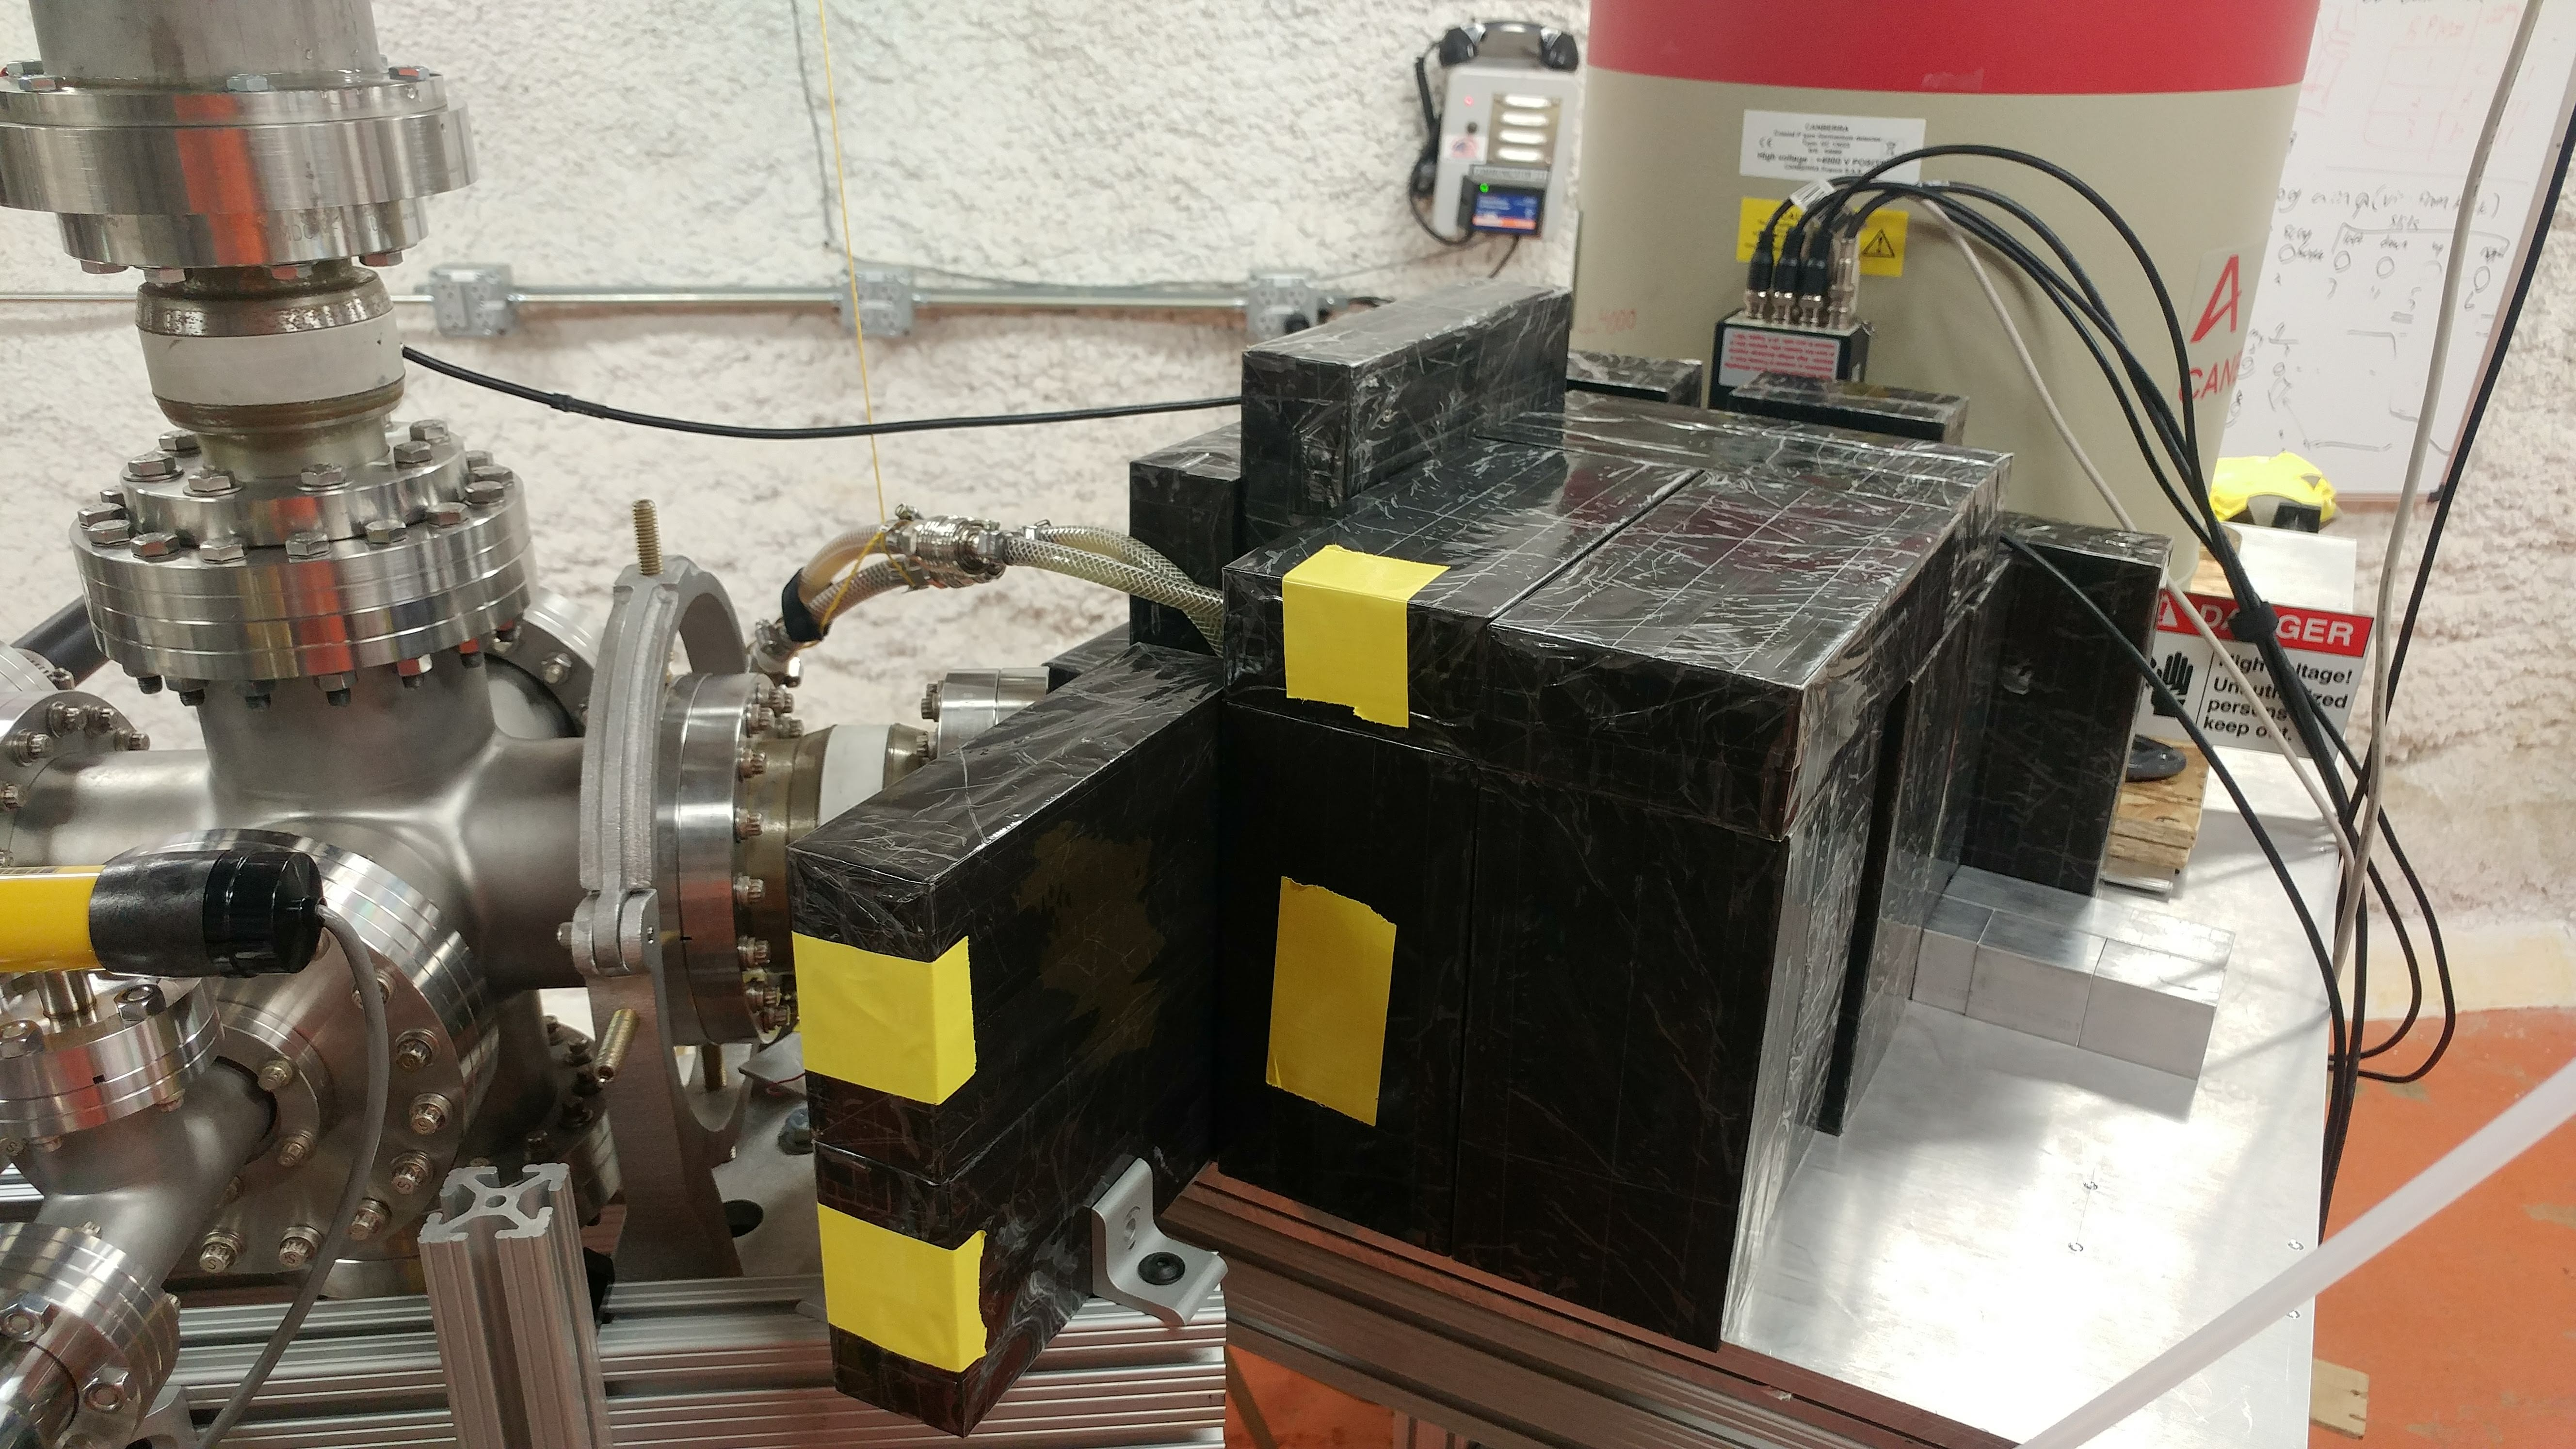
\includegraphics[width=0.8\linewidth]{figures/shieldingPicture.jpg}
\caption{A picture of the experimental setup at CASPAR, showing the lead shielding around the detector and target chamber. This figure is provided for comparison to the simulated setup to prove its accuracy. }
\label{fig: actualSetup}
\end{figure} 

To extend $\eta^{TOT}$ to the whole range of energies relevant to the experiments, the experimental setup (including the target chamber, water cooling, and shielding) was built and simulated in Geant4 \cite{Agostinelli2003}, an example of the simulation for the CASPAR setup is shown in Fig.\ \ref{fig: simulatedSetup} where the actual setup is given in Fig.\ \ref{fig: actualSetup} for comparison. Then, a single-line emission source was recreated at the target location and simulated 10,000,000 decays, recording the deposited energy inside the detector. The energy of the source was changed and simulated at energies of 662, 1300, 2000, 3000, 4000, 6000, 7000, 8000, and 10000 keV to cover the entire range of $\gamma$ ray energies present in the $^{14}$N$\left( p,\gamma \right) ^{15}$O reaction. 

Geant4 simulations are highly sensitive to detailed, accurate recreations of all aspects of the setup, including the beamline meters away or the internal structure of the detector (which isn't known). Therefore, the simulation's output was used in conjunction with the measured total efficiency data point to determine an accurate curve of the total efficiency across all experimentally relevant energies, shown in Fig.\ \ref{fig: totalEfficiency}.

\begin{figure}
\thisfloatpagestyle{plain}
\centering
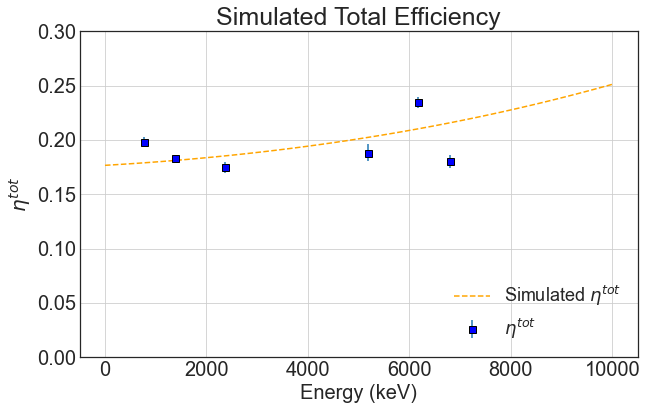
\includegraphics[width=\linewidth]{figures/totalEfficiency.png}
\caption{The total efficiency of the HPGe in the CASPAR setup across all relevant energies. The points are obtained from the transitions in the $^{14}$N$\left( p,\gamma \right) ^{15}$O reaction while the line is determined from a Geant4 simulation across the relevant energies to interpolate the total efficiency. Further details can be found in Sec. \ref{subsec: totEff}. }
\label{fig: totalEfficiency}
\end{figure}



\subsection{Peak efficiency}

The full-energy peak (FEP) efficiency, on the other hand, is the probability that the full energy of a given photon will be recorded within the detector. Mathematically, this is

\begin{equation}
\eta^{FEP} = \dfrac{n(E)}{R(E)}
\end{equation}

\noindent where $n(E)$ is the count rate in the measured peak at an energy, $E$, where $R(E)$ is the rate at which photons of energy $E$ are emitted from the source \cite{DebertinHelmerBook}. From this point, if not specified, efficiency as a term is used to denote the FEP efficiency whereas the total efficiency will always be named explicitly. 

Determining the efficiency for a given setup is necessary for each geometry since, like the total efficiency, it is related to the specific source-detector geometry; it is not an intrinsic property of a given detector. In this campaign of experiments, the efficiency was determined each time with a combination of radioactive sources, like $^{137}$Cs, $^{60}$Co, and $^{152}$Eu, and well-known nuclear resonances, like $^{14}$N$\left( p,\gamma \right) ^{15}$O at $E_{p}$ = 278 keV and the $^{27}$Al($p, \gamma$)$^{28}$Si resonance at $E_{p}$ = 992 keV. These reactions were chosen because, much like the energy calibration, these extend the detector's measured efficiency to a much higher energy range (up to 10.7 MeV) compared to radioactive sources. 

From radioactive sources, the detector's efficiency at a given $\gamma$ ray energy, $\eta^{FEP}(E_{\gamma})$, can be determined with

\begin{equation}
\eta^{FEP} (E_{\gamma}) = \dfrac{N_{\gamma}}{A(t) B_{\gamma} t_{live} C_{i}},
\end{equation}

\noindent where $N_{\gamma}$ is the measured number of counts in the full energy peak, $A(t)$ is the source's activity at the time of the measurement, $B_{gamma}$ is the branching ratio for the specific decay, $t_{live}$ is the live time of the measurement, and $C_{i}$ are the correction factors, if necessary. For nuclear resonances, on the other hand, $\eta^{FEP} (E_{gamma})$ is 

\begin{equation}
\eta^{FEP} (E_{\gamma}) = \dfrac{N_{\gamma}}{q B_{\gamma} R C_{i}},
\end{equation}

\noindent where $q$ is the collected charge and

\begin{equation}
R = \dfrac{\lambda_{r}^{2}}{\pi} \dfrac{\omega \gamma}{\epsilon_{sp}} \dfrac{M + m}{M} \tan^{-1} \left( \dfrac{\Delta E}{\Gamma}  \right)
\label{eqn: resonanceFactor}
\end{equation}

\noindent with $\lambda_{r}$ is the proton's de Broglie wavelength at the resonance energy, $\omega \gamma$ is the resonance strength (as defined in Chapter \ref{chap: introduction}), $\epsilon_{sp}$ is the stopping power of the target at the resonance energy, $M$ is the target atomic mass, $m$ is the projectile atomic mass, $\Delta E$ is the thickness of the target, and $\Gamma$ is the resonance width. 

For this determination, the branching ratios for the 278 keV resonance in $^{14}$N$\left( p,\gamma \right) ^{15}$O were taken from Daigle \textit{et al.} \cite{Daigle2016} where for the 992 keV resonance in $^{27}$Al($p, \gamma$)$^{28}$Si they were obtained from Antilla \textit{et al.} \cite{Antilla1977} and those from the 406 keV resonance in $^{27}$Al($p, \gamma$)$^{28}$Si are taken from Powell \textit{et al.} \cite{Powell1998}. The efficiencies were then fit with 

\begin{equation}
\eta^{FEP} = \exp \left(  \sum_{i=0}^{3} a_{i} ( \ln (E_{\gamma}))^{2}    \right),
\end{equation}

\noindent where the $a_{i}$ are fit coefficients and $E_{\gamma}$ is the $\gamma$-ray energy and the independent variable in the fit. An example of this determination for the CASPAR setup in both the close and far geometries can be seen in Fig. \ref{fig: efficiency}, with the percentage residuals shown in Fig. \ref{fig: effResiduals}. In both calculations, only statistical errors were included in the fit and the highest energy point was excluded due to summing effects, which will be discussed in more detail in the next section. This can be clearly seen as the highest energy point at close distance (1.1 cm from target) is off by an inordinately large factor. For a reference, measurements were also taken at 25.24 cm away from the target chamber, making the summing effects negligible and for these far distance data, the fit follows the data nearly perfectly. The curve for the near position efficiency, which was used in the subsequent cross-section analysis, was obtained by taking the far distance fit (which had no summing effects present) and scaling by a geometric factor to account for the difference in solid angle subtended by the detector in the two configurations. As was discussed in Section \ref{sec: angularCorrections}, the angular effects for the data are negligible and the efficiency reactions were isotropic, so correcting for the solid angle alone is sufficient. 


\begin{figure}
\centering
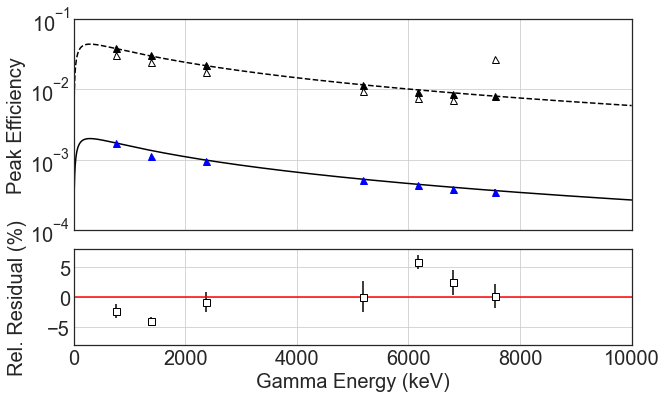
\includegraphics[width=\linewidth]{figures/efficiencyAndResiduals.png}
\caption{Top panel: detector efficiency as a function of $\gamma$-ray energy for the measurement at CASPAR in both close and far geometries, obtained from the $^{14}$N$\left( p,\gamma \right) ^{15}$O reaction. At the far distance between the detector and the target, summing effects are negligible. Therefore, the efficiency in far distance was fitted and scaled by the geometric factor to account for solid angle difference between the close and far geometries. The filled in close distance have been corrected for summing effects.  Bottom panel: relative residuals between the corrected data and the efficiency curve at the detector distance of 1.0 cm.    }
\label{fig: efficiency}
\end{figure}




\section{Summing corrections}
\label{sec: summing}

Summing corrections need to be applied to data due to data-recording phenomena manifesting in measured spectra. There are two different ways in which the recorded data can be affected, the so-called summing-in and summing-out effects, and these are more pronounced when measurements happen with the detector and source in close proximity or with simple reaction product decay structures, as in the case in the $^{14}$N$\left( p,\gamma \right) ^{15}$O reaction.


\begin{figure}
\centering
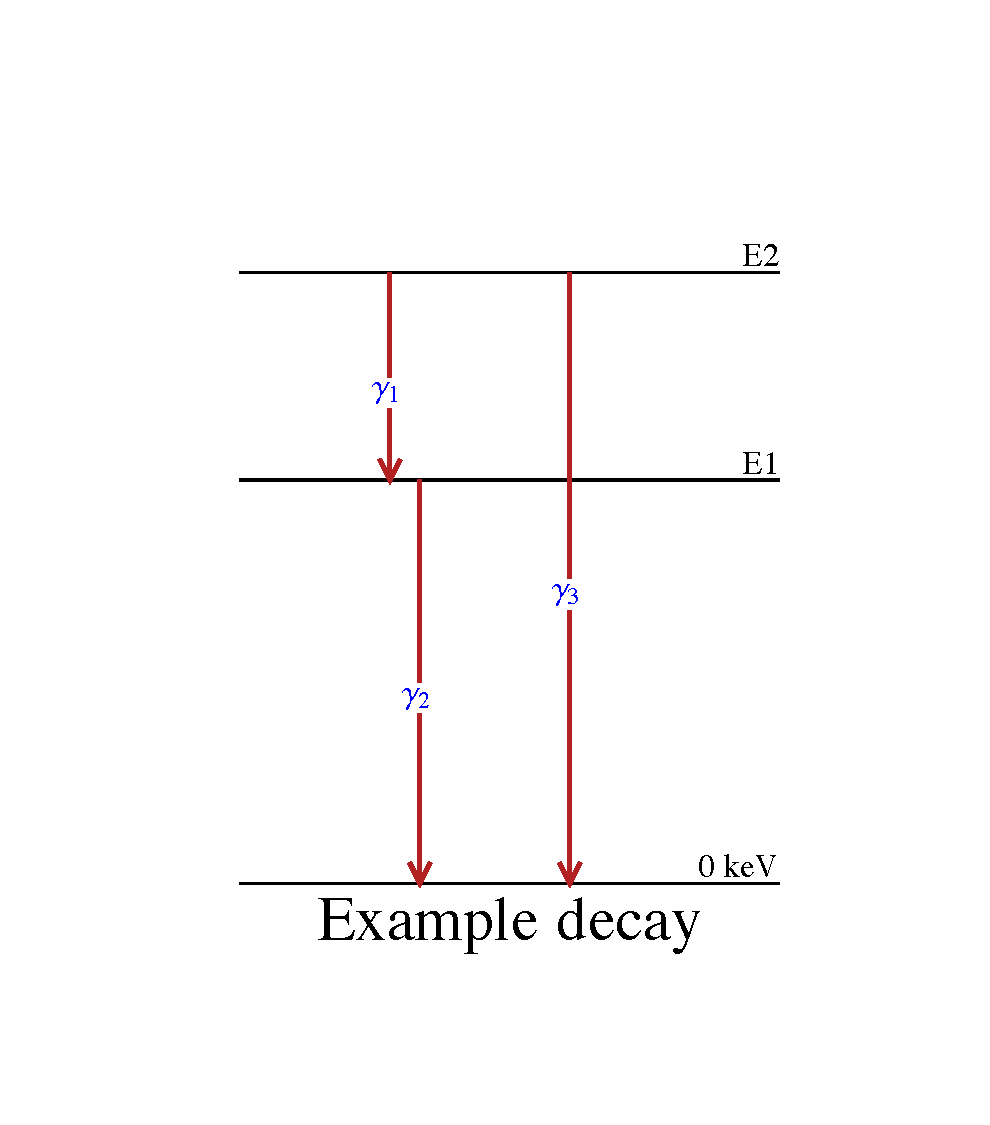
\includegraphics[width=0.7\linewidth]{figures/simpleScheme.pdf}
\caption{Example cascade nuclear decay for demonstrating summing effects (see text for details). }
\label{fig: simpleDecay}
\end{figure}

For a simple nuclear decay, like that in Fig. \ref{fig: simpleDecay}, summing manifests in a measured spectrum in two different ways. If any portion of the energy from $\gamma_{1}$ is deposited in the detector simultaneous with $\gamma_{2}$, the the resultant recorded event will have an energy higher than either individual $\gamma$-ray and, therefore, will appear at a different energy in the spectrum. Consequently, $\gamma_{2}$'s count rate will be artificially lowered. By the same logic, the count rate for $\gamma_{1}$ will also be artificially dropped. This loss of counts in the peaks recorded at energies $E_{1}$ and $E_{2}$ is known as the summing-out effect. As an extension of this thought experiment, if the full energy of both $\gamma_{1}$ and $\gamma_{2}$ is deposited in the detector at the same time the resulting measured energy will match $E_{3}$, artificially inflating the count rate of that peak. This increase is called the summing-in effect.

To correct for these effects, the probability of measuring a different energy than expected must be taken into account. For a situation where there is no summing, the rate of $\gamma$ rays is simply the yield

\begin{equation}
Y_{i} = R B_{i} \eta^{FEP}_{i},
\end{equation}

\noindent where $R$ is the normalization from Equation \ref{eqn: resonanceFactor}, $B$ is the branching ratio, and $\eta^{FEP}$ is the FEP efficiency. However, when summing-out occurs, the yield is artificially dropped by the factor $R B \eta^{FEP}_{1} \eta^{TOT}_{2}$, which is the probability of counting the full energy of $\gamma_{1}$ along with any part of $\gamma_{2}$. Mathematically, this observed yield for both $\gamma_{1}$ and $\gamma_{2}$ is

\begin{align}
Y_{1} &= R B_{1} \eta_{1} - R B_{1} \eta_{1} \eta^{tot}_{2} \\
        &= R B_{1} \eta_{1} \left( 1 - \eta^{tot}_{2} \right) \\
Y_{2} &= R B_{2} \eta_{2} \left( 1 - \eta^{tot}_{1} \right).
\end{align}

\noindent Then, in order to correct for this, the ratio of the true emitted $\gamma$'s to the observed rate for $\gamma_{1}$ is

\begin{equation}
\dfrac{Y_{1}}{Y^{obs}_{1}} = \dfrac{1}{1 - \eta^{tot}_{2}} = C_{1},
\end{equation}

\noindent where the $C_{i}$ is the correction factor. The same relation holds for $\gamma_{2}$. This makes clear why the total efficiency is so important: without it, summing-out is not an effect which can be corrected. For $\gamma_{3}$, however, the situation requires the total energy deposition of $\gamma_{1}$ and $\gamma_{2}$ at the same time, so correcting for summing-in requires the FEP efficiency. This is

\begin{equation}
Y_{3} = R B_{3} \eta_{3} + R B_{1} \eta_{1} \eta_{2}
\end{equation} 

\noindent where the second term includes $B_{1}$ because the decay chain has to start with $\gamma_{1}$. By the same token, the correction factor for summing-in is

\begin{equation}
C_{3} = \dfrac{Y_{3}}{Y_{3}^{obs}} = \dfrac{1}{1 + \left( \dfrac{B_{1} \eta_{1} \eta_{2}} {B_{3} \eta_{3}}  \right)}.
\end{equation}


With a more complicated nuclear level scheme, the summing corrections become more difficult to apply accurately. A more detailed treatment of the necessary methods can be found in \cite{DebertinHelmerBook}. This is primarily due to more complicated feeding and the presence of multiple decays from a given level. In general, the correction is for the $i$th level is

\begin{align}
C_{i} &= 1 + C_{i}^{in} - C_{i}^{out} \\
C_{i}^{in} &= \sum_{m,n} \dfrac{B_{m} p_{n} \eta_{m} \eta_{n}}{B_{i} \eta_{i}} \\
C_{i}^{out} &= \sum_{j,k} p_{k} \eta_{k}^{tot} + \dfrac{B_{j} p_{i} \eta_{j}^{tot}}{B_{i}}
\end{align}




\begin{figure}
\thisfloatpagestyle{plain}
\hspace{-2cm}
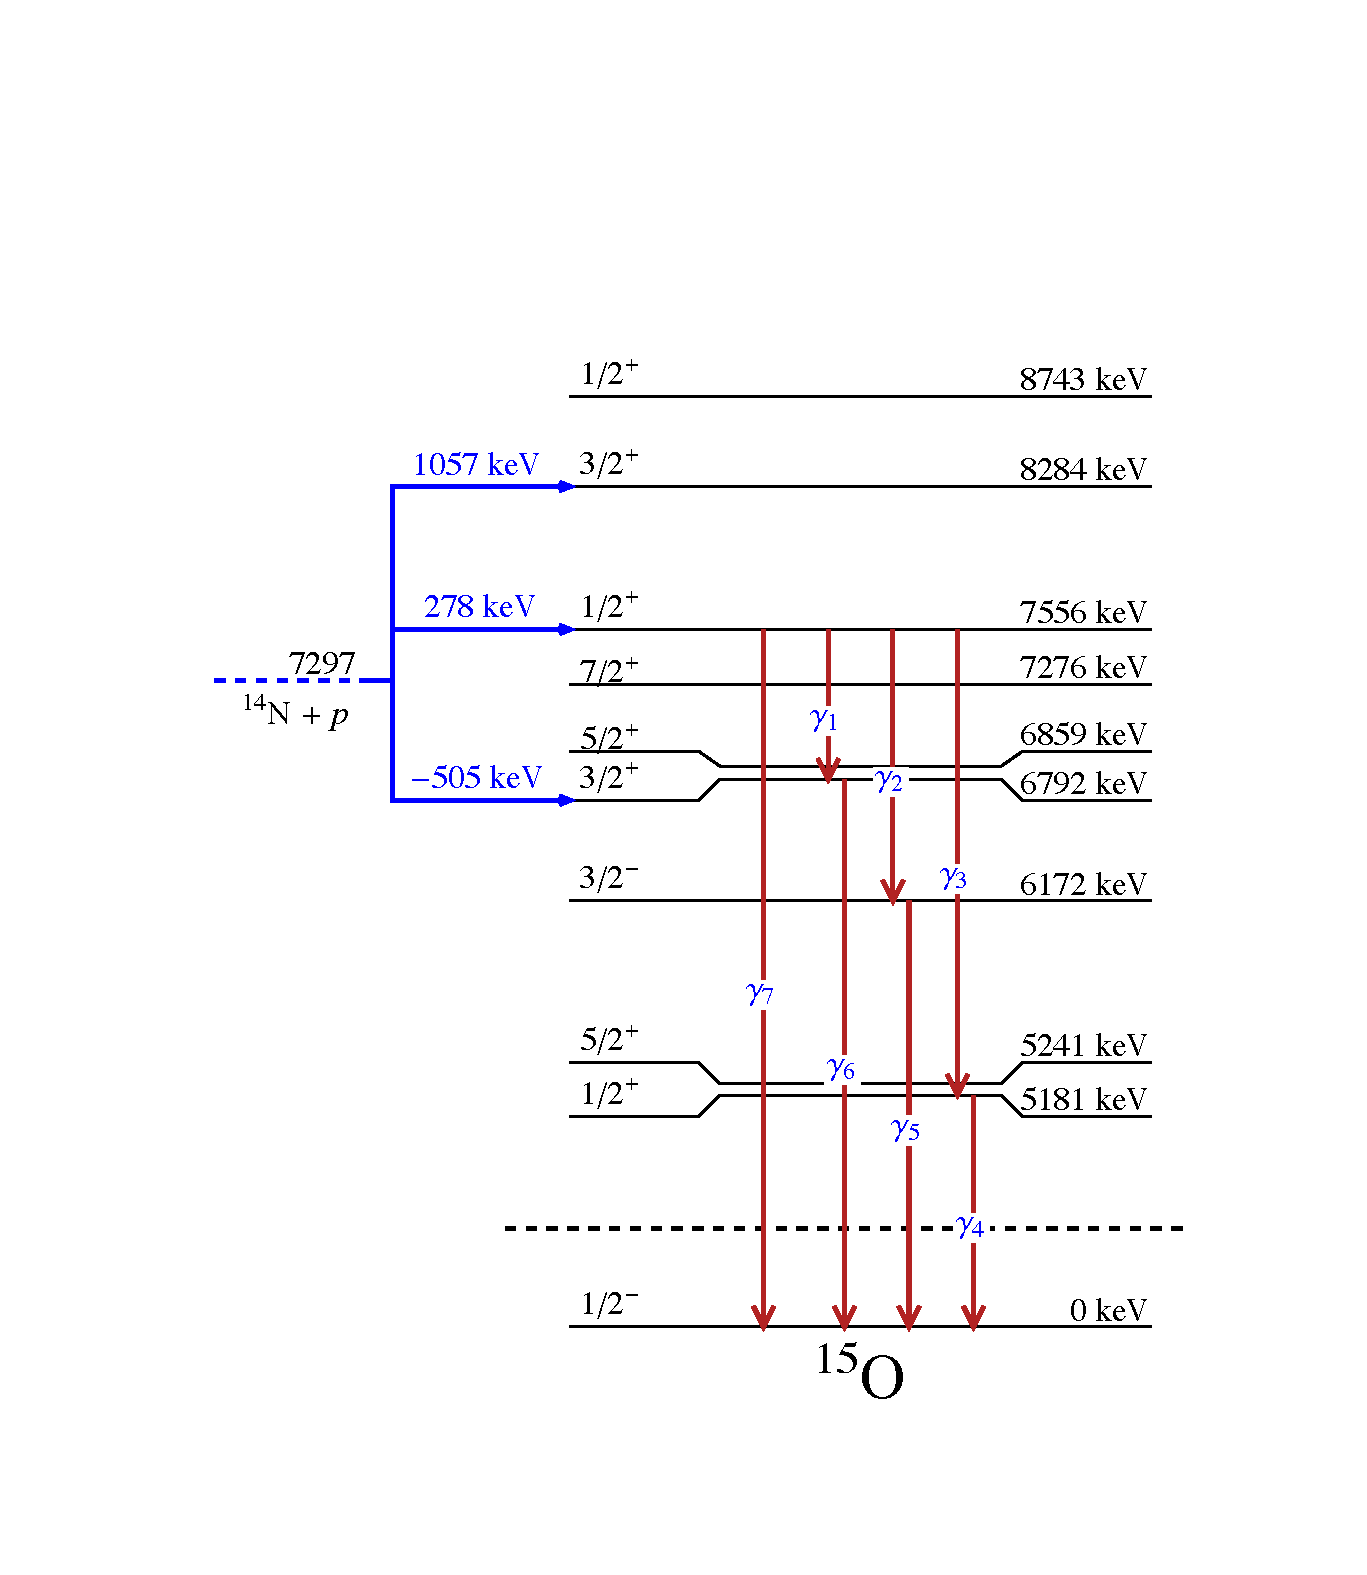
\includegraphics[width=1.0\linewidth]{figures/summingOxygenDecays.pdf}
\caption[All decays from the 278 keV proton resonance in the $^{14}$N$\left( p,\gamma \right) ^{15}$O reaction. Other than the resonance level, all decays are sequential, with the levels having only one decay directly to ground state. Of note, this then means that the total energy for each decay sequence matches the direct transition, $\gamma_{7}$, so it must be corrected for summing-in effects from all the other branches.]
{{\small All decays from the 278 keV proton resonance in the $^{14}$N$\left( p,\gamma \right) ^{15}$O reaction. Other than the resonance level, all decays are sequential, with the levels having only one decay directly to ground state. Of note, this then means that the total energy for each decay sequence matches the direct transition, $\gamma_{7}$, so it must be corrected for summing-in effects from all the other branches. }}
\label{fig: summingOxygen}
\end{figure}

\noindent where the $p_{i}$ are the probability of feeding. Fortunately, for the $^{15}$O nucleus, all intermediate decays have a branching ratio of 100\%, as can be seen in Fig.\ \ref{fig: summingOxygen}. The summing out corrections in each case can then be

\begin{equation}
C_{i}^{out} = 1 - \eta^{tot}_{j},
\end{equation}

\noindent where the $i$ and $j$ denote the $\gamma$ rays feeding into and decaying from the state, respectively (like $\gamma_{1}$ and $\gamma_{6}$ for example). For this measurement, the summing-out effect for every transition falls in the range of 28 - 32 \% for all of the relevant $\gamma$'s. %Fig.\ \ref{fig: sumOutRange} shows this, depicting the summing out correction across the range of relevant gamma energies in this experiment. 


%\begin{figure}
%		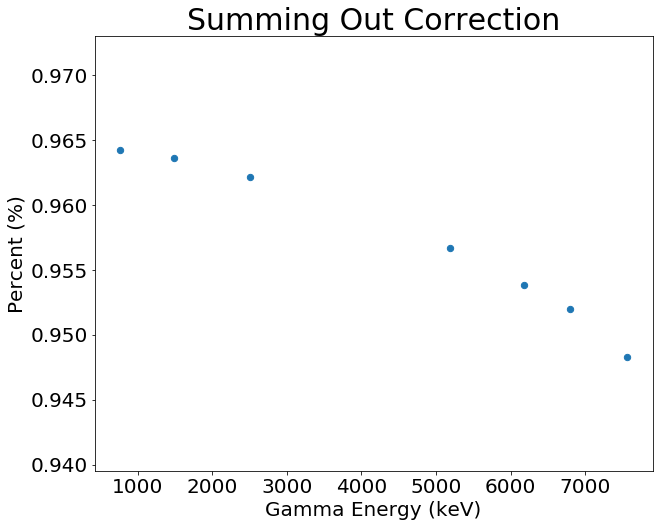
\includegraphics[width=1.0\linewidth]{figures/sumOutRange.png}
%	\caption[The summing out correction as a function of incident $\gamma$-ray energy. This figure shows the percentage of gammas recorded to the true incident number.]
%	{{\small The summing out correction as a function of incident $\gamma$-ray energy. This figure shows the percentage of gammas recorded to the true incident number.}}
%	\label{fig: sumOutRange}
%\end{figure}


Conversely, only the R/DC$\rightarrow$GS transition needs to be corrected for summing-in effects as the total energy of the other decay branches matches the energy of $\gamma_{7}$, and, as such, should be a larger effect since the true branch to the ground state is $\sim 1.5$\% \cite{Daigle2016}. The observed yield of $\gamma_{7}$ in this case will be

\begin{equation}
Y_{7} = R B_{7} \eta_{7} + R B_{1} \eta_{1} \eta_{6} +  R B_{2} \eta_{2} \eta_{5} + R B_{3} \eta_{3} \eta_{4} .
\end{equation}

\noindent From this, then, the correction factor for the ground state transition will necessarily be

\begin{equation}
C_{7}^{in} = 1 + \dfrac{B_{1} \eta_{1} \eta_{6} + B_{2} \eta_{2} \eta_{5} + B_{3} \eta_{3} \eta_{4} }{B_{7} \eta_{7}}.
\end{equation}

\noindent In this measurement, this correction is quite large, as expected. It was determined to be an approximately 80\% correction to the ground state transition in the energy range near the 278 keV resonance and as much as 61\% off the resonance.

There is a second method for calculating the summing-in correction which was also employed. This relies on the measured efficiency being taken at different distances to the source of the $\gamma$ rays on the resonance. In close geometry, the solid angle of the detector is much larger when viewed from the source and summing is present (which can be seen from the highest energy data point in the detector efficiency plot, Fig.\ \ref{fig: efficiency}). However, at a larger distance, in this case 25.4 cm, the solid angle of the detector is significantly smaller but summing-in effects are not present in the detector. Therefore, the ratio of efficiencies between the close and far distance measurements when accounting for the difference in detector solid angle is the necessary summing-in correction. 


\begin{figure}
\centering
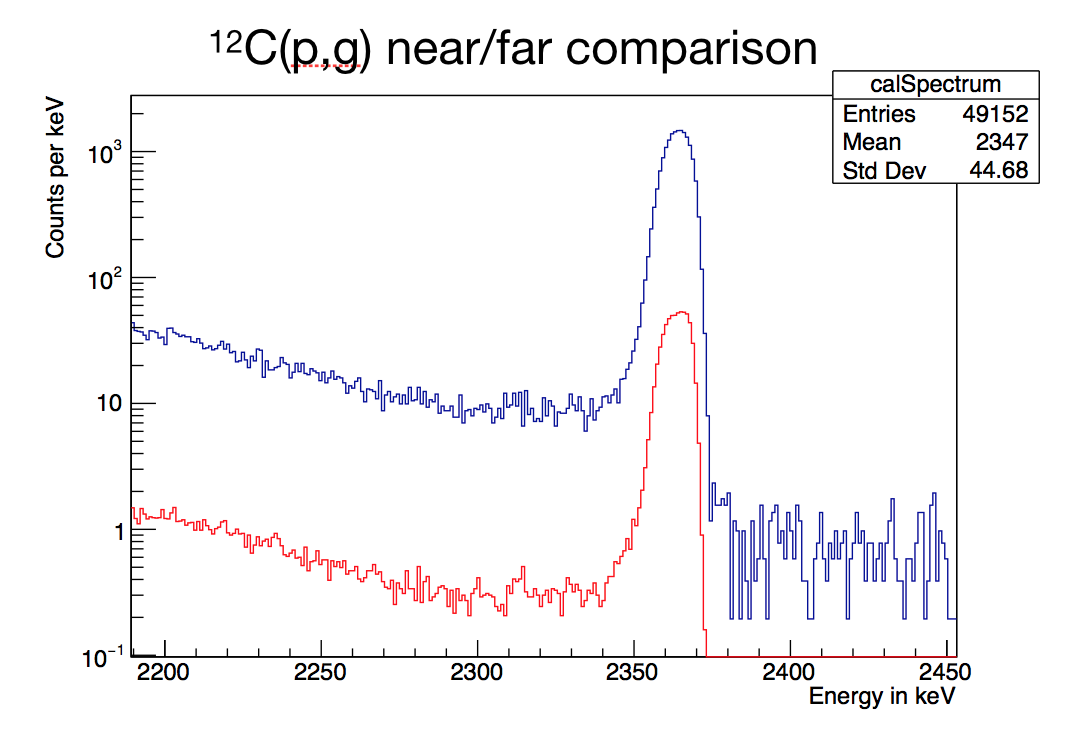
\includegraphics[width=\linewidth]{figures/carbonComparison.png}
\caption{Spectra from the $^{12}$C$\left( p,\gamma \right) ^{13}$N reaction obtained at CASPAR. The ratio of counts in the near (blue) and far (red) spectra gives us a ratio with which to correct between the near/far efficiencies. }
\label{fig: 12cpg}
\end{figure}

More accurately than calculating the solid angle geometrically, the near/far correction factor can be determined using another set of measurements with the $^{12}$C$\left( p,\gamma \right) ^{13}$N reaction. For this method, the reaction decays via a single $\gamma$ at 2.37 MeV and requires no additional correction for summing. This means that the difference between the data taken in near/far distances is due to the geometric effects and allows us to relate the efficiencies between the two measurement distances without the need for correcting for summing-out or summing-in. Spectra from the $^{12}$C$\left( p,\gamma \right) ^{13}$N reaction taken at CASPAR are shown in Fig.\ \ref{fig: 12cpg}. The ratio of counts in these two peaks gives a near/far ratio of $R_{c} = 27.8$. Using this ratio, we scale up the fitted far-efficiencies and the difference between this and the ground state peak provides the needed summing-in correction. For our data, the summing-in correction was found to be 74.6\% for the ground state transition. This agrees well with the numerically determined method in the resonance range where they overlap. This serves as good cross-validation of the summing-in correction when applying it to all of the ground state transition data.







\section{Target characterization}
\label{sec: targetCharacterization}

In order to ultimately determine the nuclear cross section and the astrophysical $S$-factor for a given reaction, the number of active atoms in the target must be known. As a reminder, the nuclear cross is a probability of interaction. The number of possible reaction sites must be known. The targets used in these measurements were sputtered TiN and ZrN targets, backed by Ta and W, respectively. By performing an energy scan over a known, thin resonance with the targets it is possible to determine the number of active atoms in the target. 

Fig. \ref{fig: yieldRes} presents a typical example of a resonance scan, which is just the measured excitation function over a resonance. This one was taken at CASPAR with the 278 keV resonance in $^{14}$N$\left( p,\gamma \right) ^{15}$O with ZrN target (\# 5) by monitoring the R $\rightarrow$ 6.79 MeV transition. Even for a monoenergetic beam, there is still a small gaussian distribution of energies encompassed in the beam (see Chapter \ref{chap: experiment} for more details). When the high energy tail of this distribution reaches the low energy side of the resonance, the measured yield from that resonance will appear. Further increasing the beam energy implies that more of the energy distribution of the beam reaches the resonance energy and the yield continues to increase. This low-energy side of the scan is referred to as the front edge and contains the intrinsic information about the resonance as well as the beam distribution. The true resonance energy, $E_{r}$ is found halfway up the front edge, 50\% of the maximum yield, because at this point a symmetric beam distribution would be half above and half below the resonance in energy. Similarly, the slope of the front edge details the energy spread in the beam, with a broader distribution corresponding to a lower slope and a tighter distribution providing a sharp front edge. 

For the incident beam particles that are above the resonance energy, they will lose energy traveling through the target and drop to energies within the resonance width and proceed through resonant capture. The maximum yield for such a scan will occur when the entire beam distribution is at an energy such that either a maximum of the ions are within the resonance width or the energy loss in the target brings a maximum number of the ions into that same range.  This maximum is known as the plateau and is the flat portion at the top of the curve in Fig. \ref{fig: yieldRes}. As a target's thickness increases the thicker this plateau becomes, since the ions will have a greater energy loss within the active target material, allowing them to decrease to resonance energy from higher and higher starting energies. For an infinitely thick target, the resonance plateau would never decrease again on the high side, because the beam would always lose enough energy to fall back into the resonance while still in the active target material. 

When targets are not infinitely thick, however, the beam energy can be increased to a point where the energy loss of the ions will eventually be such that the energy of the ions is still above the resonance width when leaving the active target material, meaning the reaction no longer proceeds through the resonant capture mechanism. When this happens, the yield starts to decrease from the level of the plateau. By a similar argument to the beam distribution leading to increased yield on the front edge, the yield on the back edge (where the plateau decreases again) drops because of the same distribution effects. The slope of this decrease is affected by the target material (leading to different energy losses) and the homogeneity (or lack thereof) of the active material. The full-width half-maximum (FWHM) of this excitation curve represents the target thickness in terms of energy loss, $\Delta E$. 



\begin{figure}
\thisfloatpagestyle{plain}
		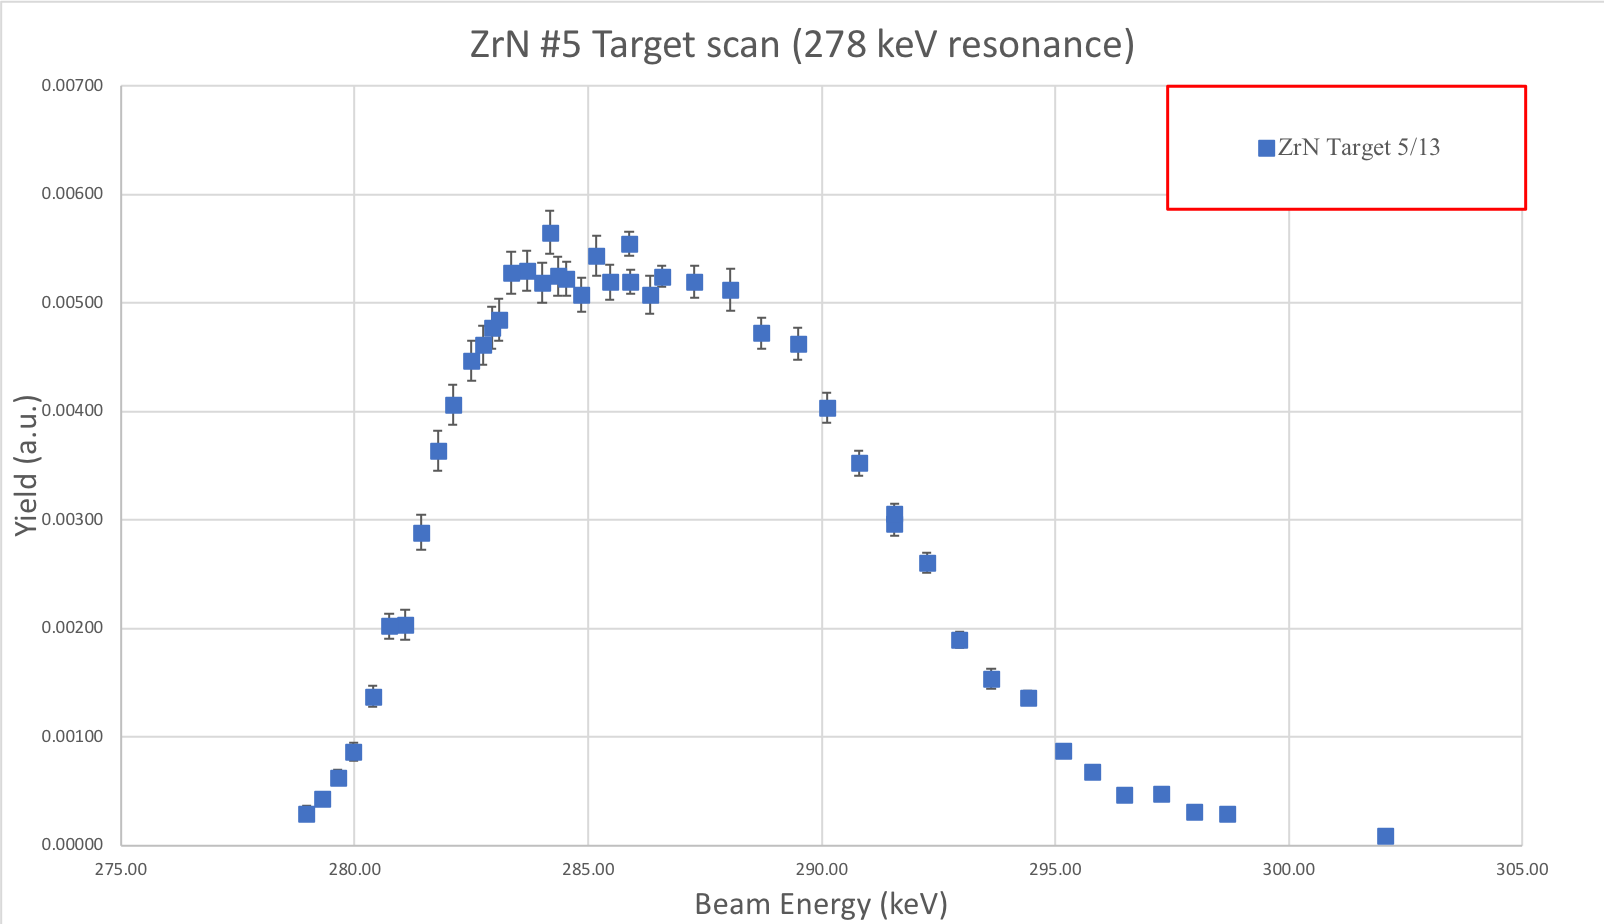
\includegraphics[width=1.0\linewidth]{figures/resScan.png}
	\caption{Resonance scan (measured Excitation curve over a resonance) taken at CASPAR with the 278 keV resonance in $^{14}$N$\left( p,\gamma \right) ^{15}$O with ZrN target (\# 5). This shows typical behavior of an energy scan over a thin resonance and from a measurement like this, the number of nitrogen atoms in the target can be determined (see text for details).}
	\label{fig: yieldRes}
\end{figure}


%There are two main methods by which the number of active atoms in a target can be determined, both of which rely on experimental scans over a thin resonance.  The targets used in these measurements were sputtered TiN and ZrN targets backed with Ta and W. 

For such a thin resonance occurring at $E_{r}$, the stopping power of the target, $\epsilon(E)$, the de Broglie wavelength, $\lambda$, and the partial widths $\Gamma_{i}$ do not change appreciably over the resonance energy. This allows the maximum yield, at $E_{0}$, to be calculated using \cite{IliadisBook}

\begin{align}
Y(E_{0}) &= \int_{E_{0}-\Delta E}^{E_{0}} \dfrac{1}{\epsilon(E)} \dfrac{\lambda^{2}}{4 \pi} \omega \dfrac{\Gamma_{a}\Gamma_{b}}{(E_{0}-E)^{2} = \Gamma^{2}/4} dE \\
           &= \dfrac{\lambda_{r}^{2}}{2 \pi} \dfrac{\omega \gamma}{\epsilon_{r}} \left[ \tan^{-1} \left(\dfrac{E_{0} - E_{r}}{\Gamma/2}  \right) - \tan^{-1} \left(  \dfrac{E_{0} - E_{r} - \Delta E}{\Gamma/2} \right)  \right].
\end{align}

Then, with some further algebraic reduction \cite{IliadisBook}, one can show

\begin{align}
E_{0} &= E_{r} + \dfrac{\Delta E}{2} \\
 Y_{max} &= \dfrac{\lambda_{r}^{2}}{\pi} \dfrac{\omega \gamma}{\epsilon_{r}} \arctan \left(\dfrac{\Delta E}{\Gamma} \right) \\
 FWHM &= \sqrt{\Gamma^{2} + \Delta E^{2}} \\
 n &= \dfrac{\Delta E}{\epsilon_{r}}, \label{eqn: targetNuclei1}
\end{align}

\noindent where $n$ is the number density of target atoms, atoms per unit area. When the target thickness, $\Delta E$ is much bigger than the resonance width, $\Gamma$, the FHWM of the resonance scan is simply the target thickness. Thus, by selecting thin resonances and determining the energy loss from their scans, like that in Fig.\ \ref{fig: yieldRes}, the number density of of active nuclei in the target can be determined with Equation \ref{eqn: targetNuclei1}. This method is useful because it does not rely on any external efficiency calibrations or corrections (since such a correction would apply to the entire curve equally, not changing the FWHM and, therefore, the thickness). Thus, this method is effective and appropriate for a uniform target material with known stoichiometry. 

The stopping powers used for these determinations were calculated using the James F. Ziegler's industry standard SRIM program, \cite{Ziegler2010}. The output from this program provides the discrete values for the stopping power of a user specified target material over a range of user specified energies. Using the stopping powers at the resonance energy in units of (eV / (atoms/cm$^{2}$)) and the overall uncertainty in the calculations of 4.6\% \cite{Ziegler2010} the number of target atoms can be determined for each resonance scan. Table \ref{tbl: targetAtoms} summarizes the results for this calculation and gives the initial number density of nitrogen atoms for the targets used throughout this experiment. 


\begin{table}[]
\caption{NITROGEN CONTENT OF TARGETS}
\centering
\begin{threeparttable}
\begin{tabular}{ll}
\toprule
Target & $n$ $\left(10^{17} \text{atoms / cm}^{2} \right)$ \\ \midrule
TiN    & 7.070 $\pm$ 0.566                        \\
ZrN \#5  & 5.647 $\pm$ 0.450                        \\
ZrN \#1  & 5.777 $\pm$ 0.466                        \\
ZrN \#12 & 10.480 $\pm$ 0.834                       \\ \bottomrule
\end{tabular}
\begin{tablenotes}
\small
\item Active nitrogen target atoms for each of the targets used as a part of this measurement. 
\end{tablenotes}
\end{threeparttable}
\label{tbl: targetAtoms}
\end{table}


However, by delivering more beam to the targets, more of the active material is removed and the targets degrade. In order to account for this effect, multiple resonance scans were taken using the different targets at different points in the experiments in order to determine the number of active target atoms throughout the measurement. By taking the initial scans as baseline values and comparing the target thickness as a function of charge delivered a linear relationship can be deduced. Fig.\ \ref{fig: targetThicknesses} shows the deterioration of the targets as a function of the delivered charge throughout the experiment and the linear fits to these data. These relationships can then be used to independently correct the individual measured runs for the accumulated charge on the target up to that particular point. 

\begin{figure}
\thisfloatpagestyle{plain}
     \centering
        \begin{subfigure}[b]{0.475\textwidth}
            \centering
            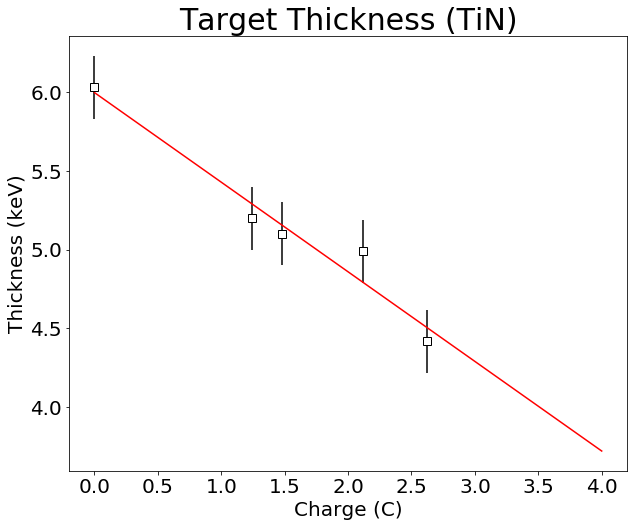
\includegraphics[width=\textwidth]{figures/targetThickness0.png}
            \caption[TiN sputtered target]%
            {{\small TiN sputtered target}}    
            \label{fig: target0}
        \end{subfigure}
        \hfill
        \begin{subfigure}[b]{0.475\textwidth}  
            \centering 
            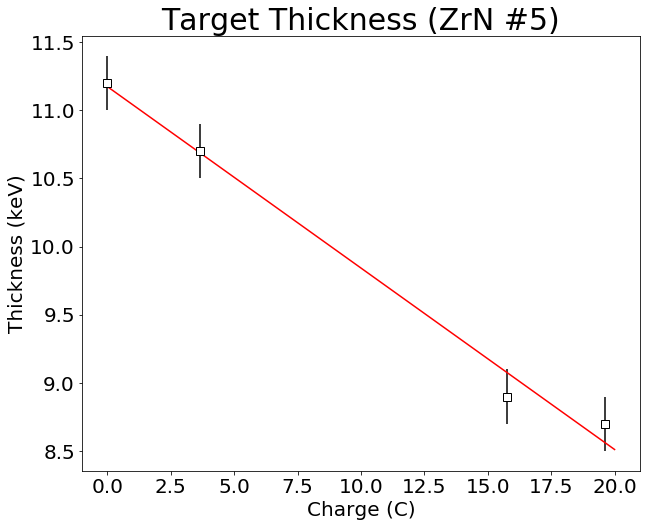
\includegraphics[width=\textwidth]{figures/targetThickness5.png}
            \caption[ZrN sputtered target 5]%
            {{\small ZrN sputtered target 5}}    
            \label{fig: target5}
        \end{subfigure}
        \vskip\baselineskip
        \begin{subfigure}[b]{0.475\textwidth}   
            \centering 
            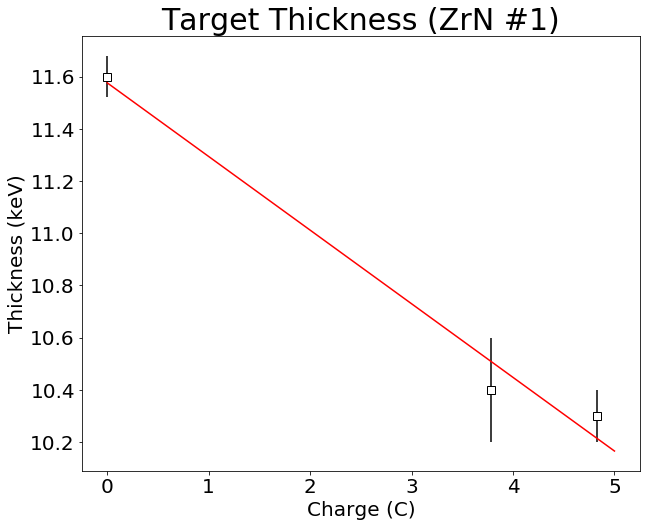
\includegraphics[width=\textwidth]{figures/targetThickness1.png}
            \caption[ZrN sputtered target 1]%
            {{\small ZrN sputtered target 1}}    
            \label{fig: target1}
        \end{subfigure}
        \quad
        \begin{subfigure}[b]{0.475\textwidth}   
            \centering 
            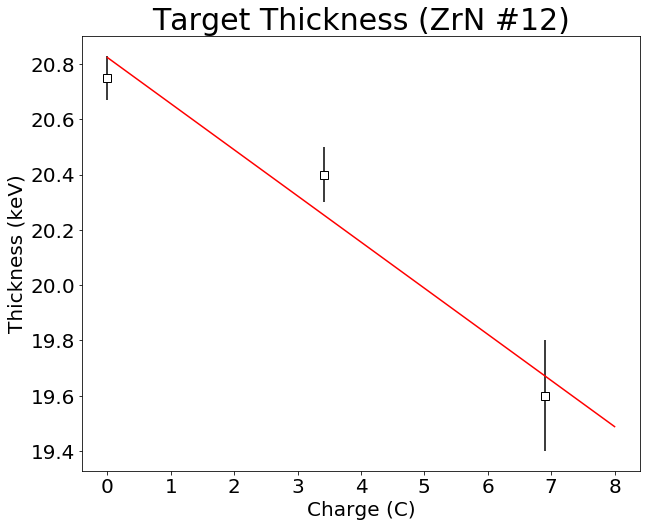
\includegraphics[width=\textwidth]{figures/targetThickness12.png}
            \caption[ZrN sputtered target 12]%
            {{\small ZrN sputtered target 12}}    
            \label{fig: target12}
        \end{subfigure}
        \caption[ The thicknesses of the various targets used in this experiment as a function of the charge delivered. This shows the deterioration of the targets through the course of the experiment where the thickness was monitored by scanning known resonances. ]
        {\small The thicknesses of the various targets used in this experiment as a function of the charge delivered. This shows the deterioration of the targets through the course of the experiment where the thickness was monitored by scanning known resonances. } 
        \label{fig: targetThicknesses}
\end{figure}




\section{Cross section determination}
\label{sec: cross-section}


In the following analysis, the differential cross section determination for each of the measured transitions follows the same procedure with the different individual correction factors for each of the transitions. Therefore, without loss of generality, they all occur according to the following procedure.

The yield of each transition, $Y_{i}$, is the number of reactions per incident projectile (protons, in this case). It was calculated by 

\begin{equation}
Y_{i} = \dfrac{N_{\gamma} C_{in}}{\eta N_{p} C_{out}},
\label{eqn: yieldCalc}
\end{equation}

\noindent where $N_{\gamma}$ is the measured number of $\gamma$-rays at the energy corresponding to the transition of interest, $C_{in}$ and $C_{out}$ are the summing in and out corrections, respectively, $N_{p}$ is the number of protons measured on target throughout the run, and $\eta$ is the detector efficiency at the measured $\gamma$ ray energy, $E_{\gamma}$. The uncertainty in this yield arises from the uncertainties in the counts of the $\gamma$-ray peak and the efficiency. In the case of the off-resonance region of the cross section, the uncertainty in the number of counts is the dominant term. These uncertainties are propagated through the yield calculation for each individual data point.

The experimental yield at a given incident proton energy, $Y(E_{p})$, corresponds to the differential cross section, $\dfrac{d \sigma}{d \Omega}$, integrated over the target thickness, $\Delta E$:

\begin{equation}
Y(E_{p}) = \int_{E_{p} - \Delta E}^{E_{p}} \dfrac{d \sigma(E)}{d \Omega} \dfrac{1}{\epsilon(E_{p})} dE,
\label{eqn: yieldCS}
\end{equation}

\noindent where, again, $\epsilon$ is the target's stopping power at the incident proton energy. 

For a thick target, the yield on top of a resonance can be written as

\begin{equation}
Y_{max}(\infty) = \dfrac{\lambda_{R}^{2}}{2} \dfrac{\omega \gamma}{\epsilon_{R}},
\end{equation}

\noindent where $\lambda_{R}$ is the de Broglie wavelength in the center-of-mass system and $\omega \gamma$ is the resonance strength. 



In determining the cross section for non-resonant regions, the thin target relation is useful because the cross section is approximately constant over the target thickness. The yield for such situation, then, becomes

\begin{equation}
Y_{NR}(E) = \dfrac{d \sigma}{d \Omega} \dfrac{\Delta(E_{p})}{\epsilon(E_{p})}
\end{equation}

\noindent where $\Delta(E_{p})$ is the target thickness in terms of energy for an incident beam of energy $E_{p}$ and NR denotes non-resonant. This can be rearranged in terms of the cross section

\begin{equation}
\dfrac{d \sigma}{d \Omega} = \dfrac{Y_{NR} \epsilon(E_{p})}{\Delta(E_{p})} = \dfrac{Y_{NR}}{N_{T}} = \dfrac{N_{\gamma}C_{in}} {\eta  N_{p} C_{out} N_{T}},
\label{eqn: thinTargetCS}
\end{equation}

\noindent where $N_{T}$ is the number of active target nuclei (in this case, nitrogen). In order to make calculations easier, this can be further reduced by factoring the infinitely-thick yield from resonance measurements by

\begin{eqnarray}
\dfrac{d \sigma}{d \Omega} &=& \dfrac{Y_{NR} \epsilon(E_{p})}{\Delta(E_{p})} \dfrac{Y_{max}(\infty)}{Y_{max}(\infty)} \\
   &=& \dfrac{\lambda_{R}^{2}}{2} \dfrac{\omega \gamma}{\epsilon_{R}} \dfrac{\epsilon(E_{p})}{\Delta(E_{p})} \dfrac{Y_{NR}}{Y_{max}(\infty)} \\
   &=& \dfrac{\lambda_{R}^{2}}{2} \dfrac{\omega \gamma}{\Delta(E_{p})} \dfrac{Y_{NR}}{Y_{max}(\infty)} 
\end{eqnarray}

\noindent This allows an experimental determination of the cross section by using only the de Broglie wavelength, which can be calculated from the experimental parameters, the resonance strength, which has been previously determined \cite{Imbriani2005, Daigle2016}, the target thickness, and the relative yields between non-resonant capture data with the yield on a known resonance (in this case, the $E_{p}$ = 278 keV resonance). 


This is the method by which the differential cross section of the $^{14}$N$\left( p,\gamma \right) ^{15}$O reaction was determined for the different transitions. The uncertainty on this differential cross section was calculated for each individual point by propagating the uncertainty in the number of nitrogen atoms with the uncertainty in the calculated yields. This also took into account the loss of nitrogen within the targets over the course of the experiment (see Sec.\ \ref{sec: targetCharacterization} for details). The resulting differential cross sections are shown in Figs.\ \ref{fig: cs679_targs} and \ref{fig: csGS_targs}. 



\begin{figure}
\thisfloatpagestyle{plain}
		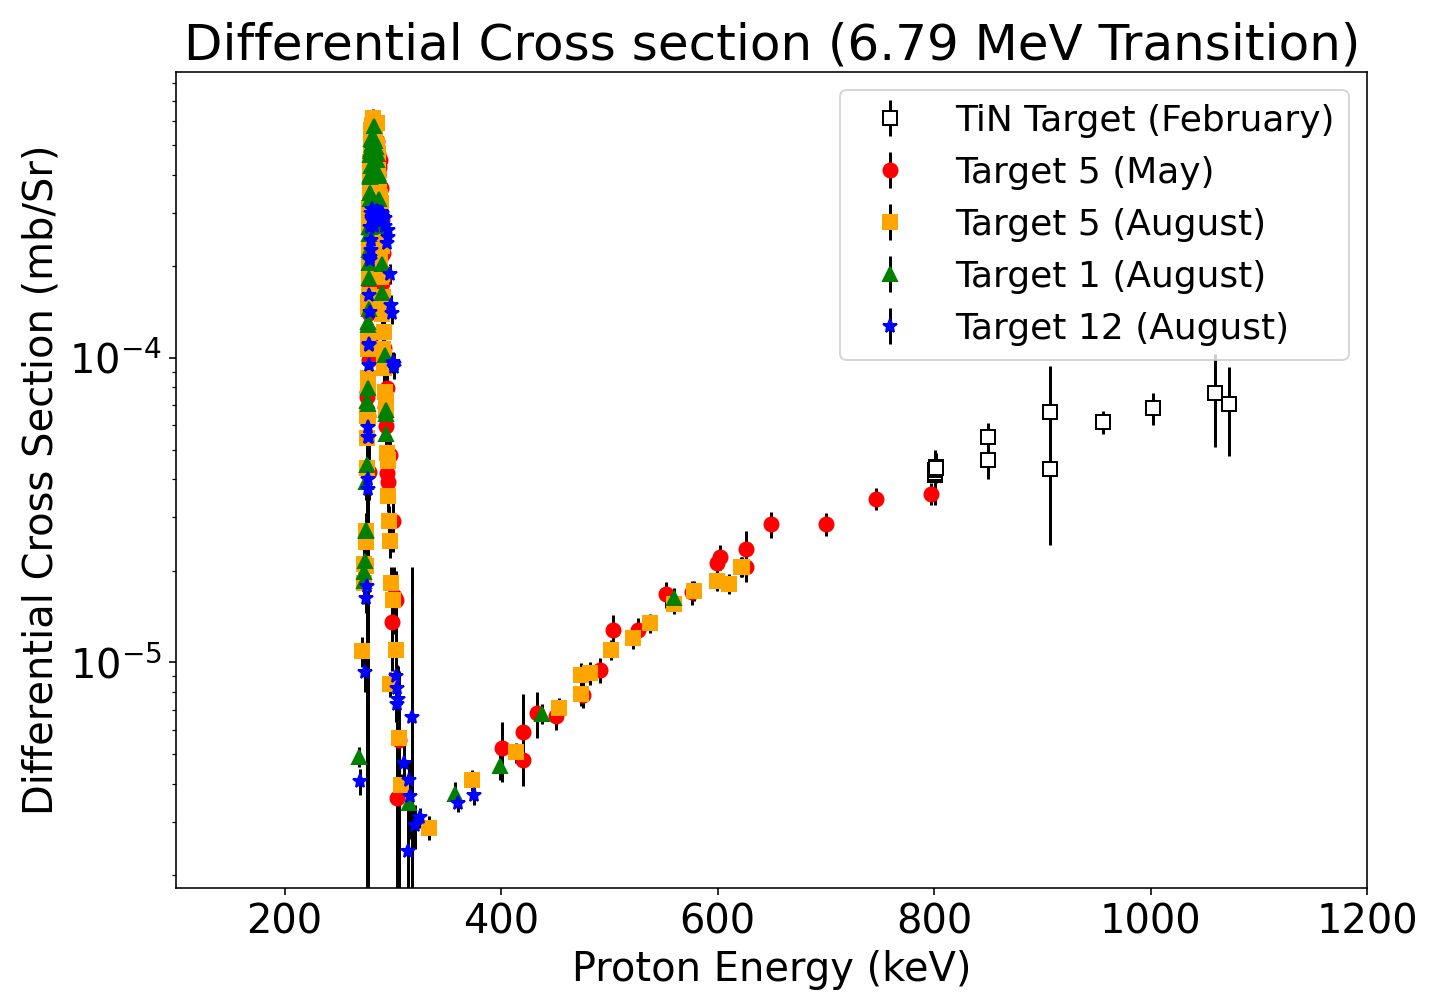
\includegraphics[width=1.0\linewidth]{figures/cs679_targs.png}
	\caption{Differential cross section for the 6.79 MeV transition in the $^{14}$N$\left( p,\gamma \right) ^{15}$O reaction, separated by the target used in measurements, showing the overlapping measurements and agreement between them. The target labels are nominal and do not represent the properties of the target, but targets 1 and 5 were the same thickness while target 12 was roughly double.}
	\label{fig: cs679_targs}
\end{figure}

\begin{figure}
\thisfloatpagestyle{plain}
		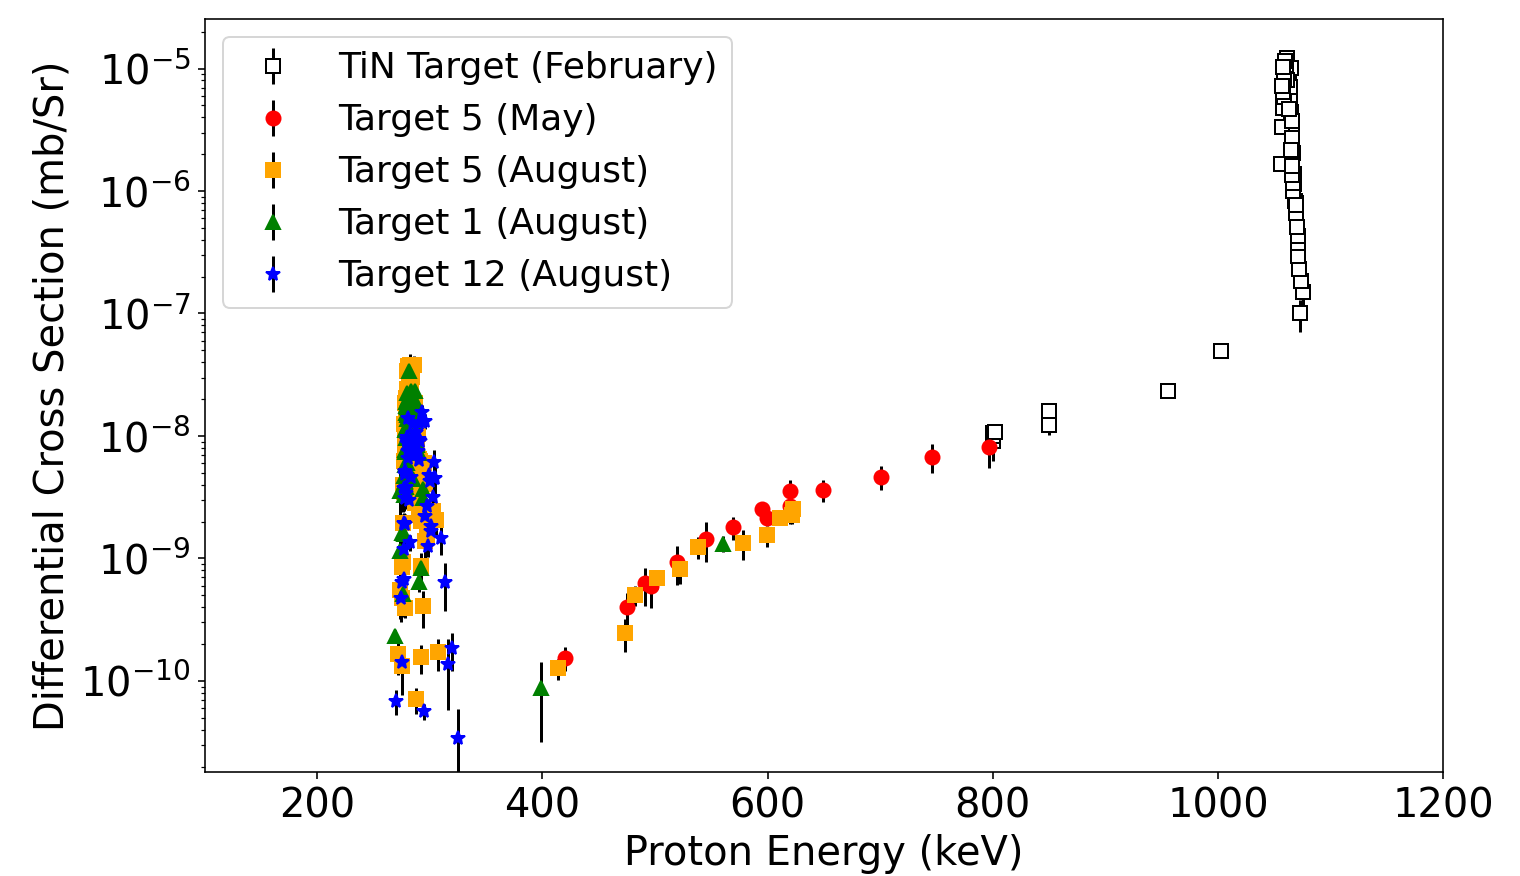
\includegraphics[width=1.0\linewidth]{figures/cs_gs_targs.png}
	\caption{Differential cross section for the ground state transition in the $^{14}$N$\left( p,\gamma \right) ^{15}$O reaction, separated by the target used in measurement, showing the overlapping measurements and agreement between them. The target labels are nominal and do not represent the properties of the target, but targets 1 and 5 were the same thickness while target 12 was roughly double.}
	\label{fig: csGS_targs}
\end{figure}




In order to move from differential measurements to a total cross section or total $S$-factor, as well as extrapolate to the Gamow window, an $R$-matrix calculations were performed with the \texttt{AZURE2} software \cite{Azuma2010}. A full description of this and incorporating the lifetime results into this analysis are presented later in Chapter \ref{chap: r-matrix}. Within the calculations, our data and the data from \citet{Li2016} are treated as differential. To compare our results alongside those from literature data \cite{Schroder1987, Imbriani2005, Runkle2005, Li2016, Wagner2018}, we scaled the resulting $S$-factors by $4\pi$ for plotting only.  These comparisons can be seen in the series of Figs.\ \ref{fig: full679} - \ref{fig: lowGS}. 


For the 6.79 MeV transition, the data are shown in Fig.~\ref{fig: full679} - \ref{fig: low679}. Our measurement agrees well with the data from \citet{Schroder1987} and \citet{Li2016} coming in from higher energies but is lower than the data from \citet{Wagner2018}. Our highest uncertainty data points overlap with the data from \citet{Wagner2018} but are otherwise discrepant. Our results agree well with the literature data in the lower-energy region where the results from LUNA \cite{Formicola2004, Imbriani2005, Marta2008, Marta2011} and LENA \cite{Runkle2005} made their measurements. Some of our data shows higher uncertainties at lower energies than other, measured data, but they agree well. Unlike the ground state data, the measurements for this transition stop at $\sim 1$ MeV. The runs at these energies were not done long enough to have appreciable statistics in the 6.79 peak. The resonance at this energy populates the ground state strongly and that was the focus of the measurement at those energies. This same lack of statistics is why the data points at 850 keV and 1000 keV also have comparatively larger uncertainties. These features can be seen highlighted in Fig.\ \ref{fig: highCompare679}, while the measured $S$-factor data for this transition in different energy regimes is plotted in Figs.\ \ref{fig: full679}, \ref{fig: highCompare679}, and \ref{fig: low679}.


\begin{figure}
\thisfloatpagestyle{plain}
		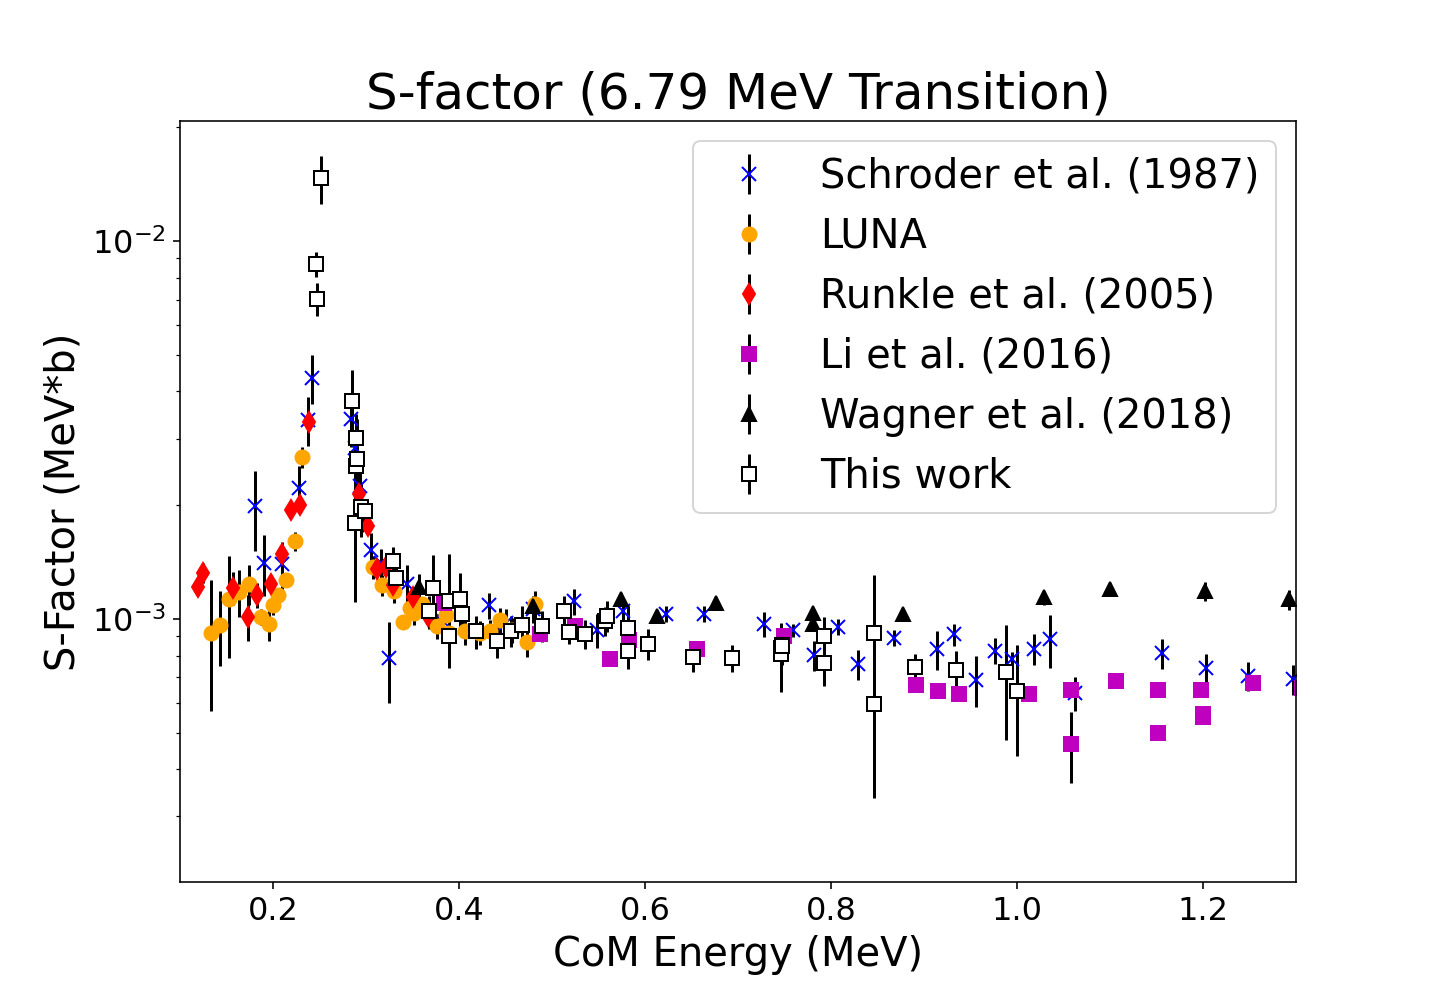
\includegraphics[width=1.0\linewidth]{figures/full679.png}
	\caption{$S$-factor for the 6.79 MeV transition in the $^{14}$N$\left( p,\gamma \right) ^{15}$O reaction for the entire energy range measured in this experiment. Also plotted are data from \cite{Schroder1987, Formicola2004, Imbriani2005, Runkle2005, Marta2008, Marta2011, Li2016, Wagner2018} for comparison. The LUNA data specifically represents the measurements \cite{Formicola2004, Imbriani2005, Marta2008, Marta2011}. Our data and that from \citet{Li2016} were both calculated as differential $S$-factors but scaled up by a factor of $4\pi$ for plotting purposes.  }
	\label{fig: full679}
\end{figure}

\begin{figure}
\thisfloatpagestyle{plain}
		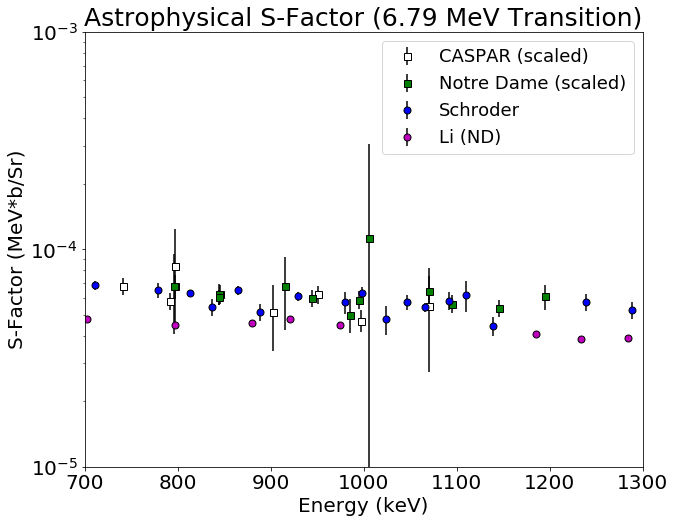
\includegraphics[width=1.0\linewidth]{figures/highCompare679.png}
	\caption{Differential cross section for the 6.79 MeV transition in the $^{14}$N$\left( p,\gamma \right) ^{15}$O reaction, highlighting the high energy region to compare the data taken at CASPAR to literature data in this region. The literature data plotted are taken from \cite{Schroder1987, Li2016, Wagner2018} for comparison. Our data and that from \citet{Li2016} were both calculated as differential $S$-factors but scaled up by a factor of $4\pi$ for plotting purposes.  }
	\label{fig: highCompare679}
\end{figure}

\begin{figure}
\thisfloatpagestyle{plain}
		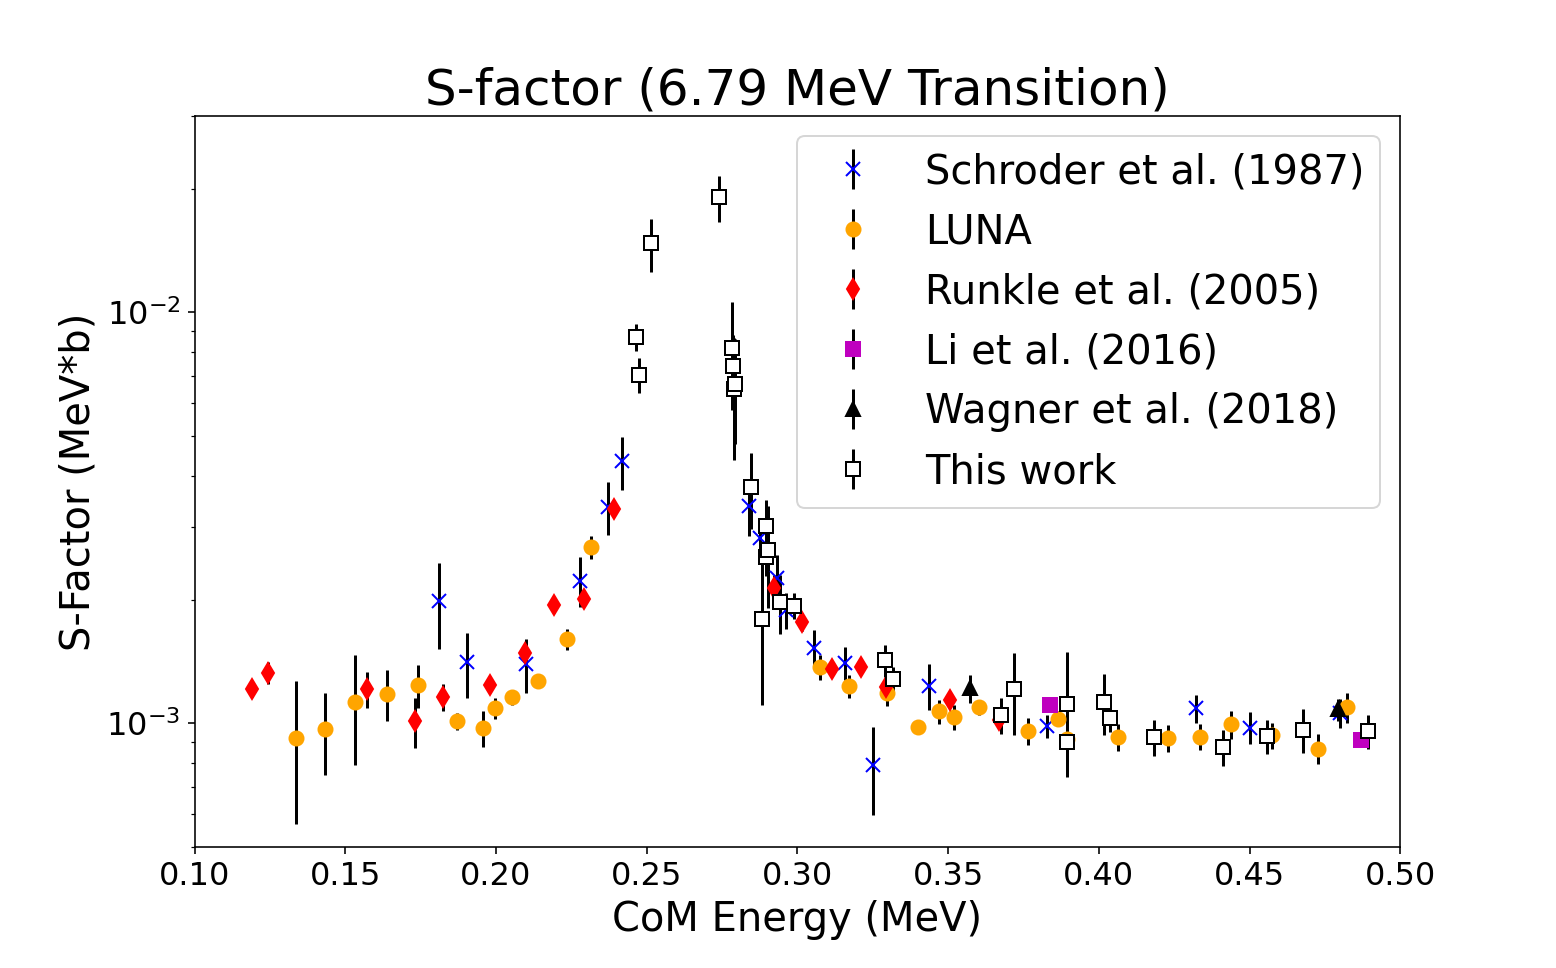
\includegraphics[width=1.0\linewidth]{figures/low679.png}
	\caption{Differential cross section for the 6.79 MeV transition in the $^{14}$N$\left( p,\gamma \right) ^{15}$O reaction, showing the behavior at low energy. Also plotted are data from \cite{Schroder1987, Formicola2004, Imbriani2005, Runkle2005, Marta2008, Marta2011, Li2016, Wagner2018} for comparison. The LUNA data specifically represents the measurements \cite{Formicola2004, Imbriani2005, Marta2008, Marta2011}. Our data and that from \citet{Li2016} were both calculated as differential $S$-factors but scaled up by a factor of $4\pi$ for plotting purposes. }
	\label{fig: low679}
\end{figure}

For the ground state transition, the data is shown in Figs.~\ref{fig: fullGS} - \ref{fig: lowGS} alongside those from Refs. \cite{Schroder1987, Formicola2004, Imbriani2005, Runkle2005, Marta2008, Marta2011, Li2016, Wagner2018}. Our measurement is in very good agreement with all reported literature data. At energies above 800 keV, shown in Fig. \ref{fig: highCompareGS}, our data overlaps perfectly with that from \citet{Schroder1987} and \citet{Li2016}. Our measured $S$-factor drops below the other reported measurements between 800 keV and 600 keV. At energies below this point, our data agrees well with the published data from \citet{Runkle2005} and the LUNA data \cite{Formicola2004, Imbriani2005, Marta2008, Marta2011}, although it has larger uncertainties. In the region between 300-500 keV, right above the resonance, our data continues to agree well with literature. However, our data becomes noticably sparser in this energy regime. WIth such low statistics in the data for these points, most had uncertainties greater than 100\% after accounting for all sources of uncertainty and were excluded. The few points that we were able to successfully take below the 278 keV resonance are in good agreement with the data taken by the LUNA group. Overall, this data shows higher uncertainties than the literature data and our own  6.79 MeV transition data. This is because this is a much more weakly populated transition and it was not feasible to run long enough to achieve appreciable statistics in the $\gamma$-ray data at these energies. Therefore, they have uncertainties dominated by the rate of measured $\gamma$'s in the experiment. Ultimately, this is a robust data set showing excellent agreement with previously published data.





\begin{figure}
\thisfloatpagestyle{plain}
		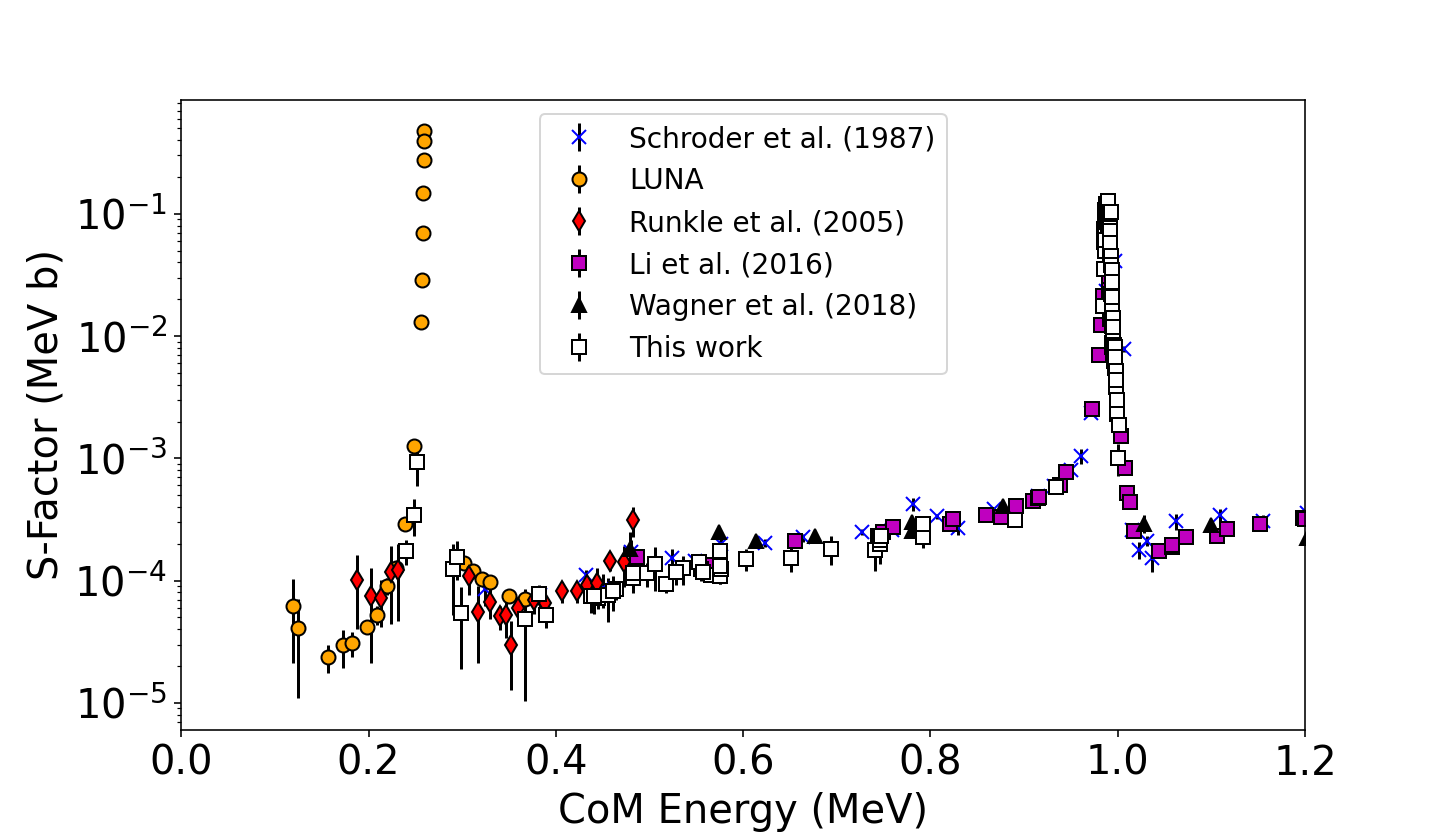
\includegraphics[width=1.0\linewidth]{figures/full_gs.png}
	\caption{Differential $S$-factor for the ground state transition in the $^{14}$N$\left( p,\gamma \right) ^{15}$O reaction for the entire energy range measured in this experiment. Also plotted are data from \cite{Schroder1987, Formicola2004, Imbriani2005, Runkle2005, Marta2008, Marta2011, Li2016, Wagner2018} for comparison. The LUNA data specifically represents the measurements \cite{Formicola2004, Imbriani2005, Marta2008, Marta2011}. Our data and that from \citet{Li2016} were both calculated as differential $S$-factors but scaled up by a factor of $4\pi$ for plotting purposes. }
	\label{fig: fullGS}
\end{figure}

%\begin{figure}
%\thisfloatpagestyle{plain}
%		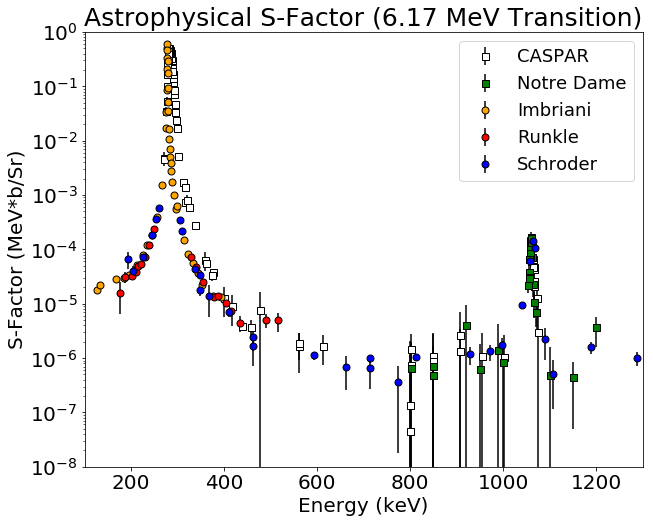
\includegraphics[width=1.0\linewidth]{figures/full617.png}
%	\caption{Differential $S$-factor for the 6.17 MeV transition in the $^{14}$N$\left( p,\gamma \right) ^{15}$O reaction for the entire energy range measured in this experiment. Also plotted are data from \cite{Schroder1987, Imbriani2005, Runkle2005, Li2016} for comparison.  }
%	\label{fig: full617}
%\end{figure}



\begin{figure}
\thisfloatpagestyle{plain}
		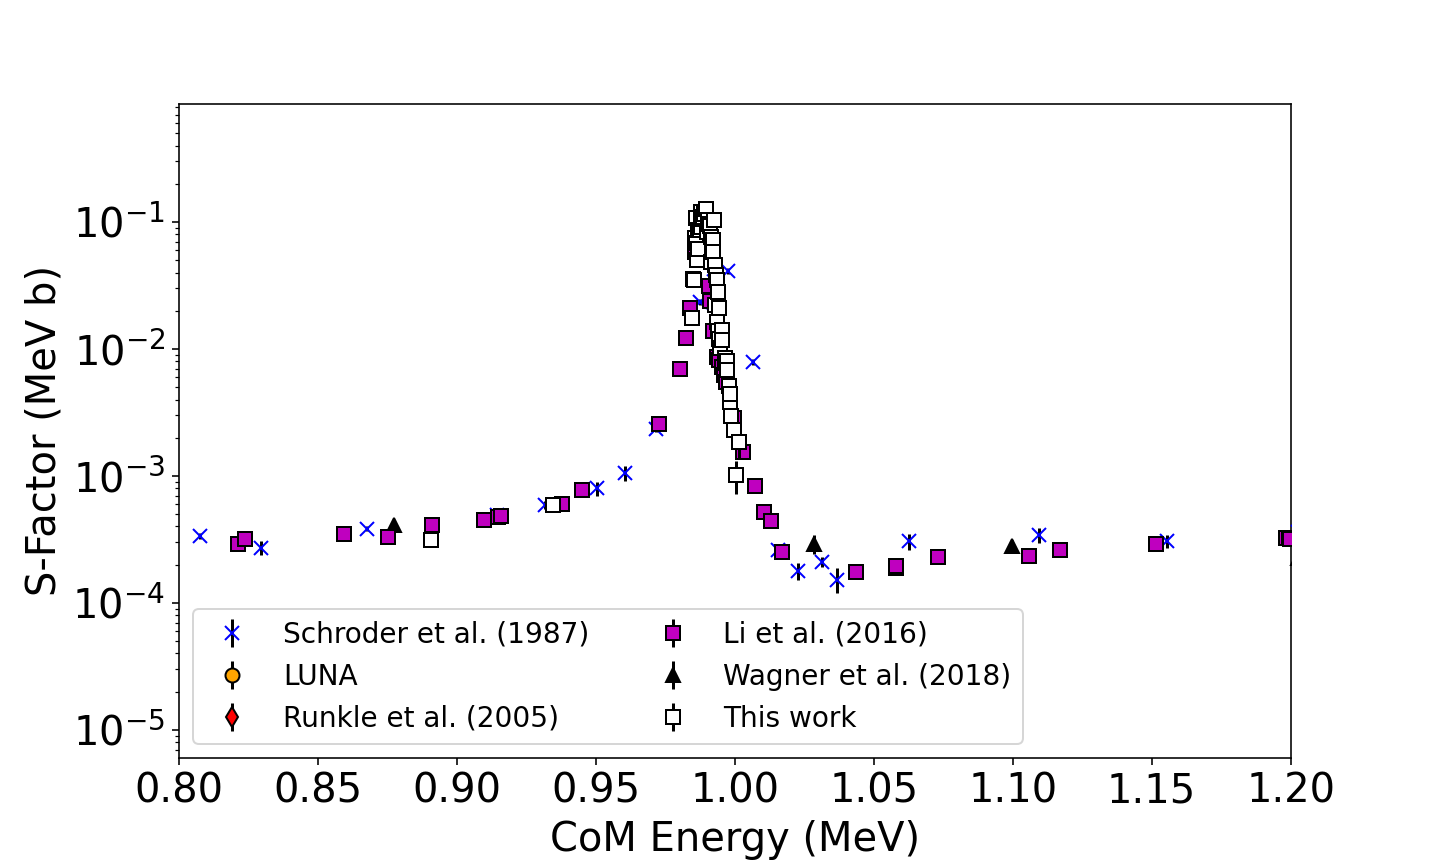
\includegraphics[width=1.0\linewidth]{figures/high_gs.png}
	\caption{Differential cross section for the ground state transition in the $^{14}$N$\left( p,\gamma \right) ^{15}$O reaction highlighting the high energy region to compare the data taken at CASPAR to literature data in the same region. Also plotted are data from \cite{Schroder1987, Li2016, Wagner2018} for comparison. Our data and that from \citet{Li2016} were both calculated as differential $S$-factors but scaled up by a factor of $4\pi$ for plotting purposes.  }
	\label{fig: highCompareGS}
\end{figure}

%\begin{figure}
%\thisfloatpagestyle{plain}
%		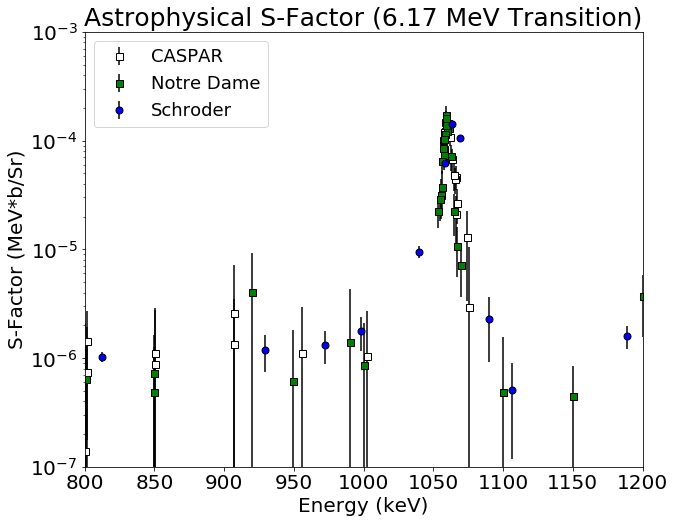
\includegraphics[width=1.0\linewidth]{figures/highCompare617.png}
%	\caption{Differential cross section for the 6.17 MeV transition in the $^{14}$N$\left( p,\gamma \right) ^{15}$O reaction highlighting the high energy region to compare the data taken at the NSL to CASPAR, showing the efficacy of the facility. Also plotted are data from \cite{Schroder1987, Li2016} for comparison.  }
%	\label{fig: highCompare617}
%\end{figure}


\begin{figure}
\thisfloatpagestyle{plain}
		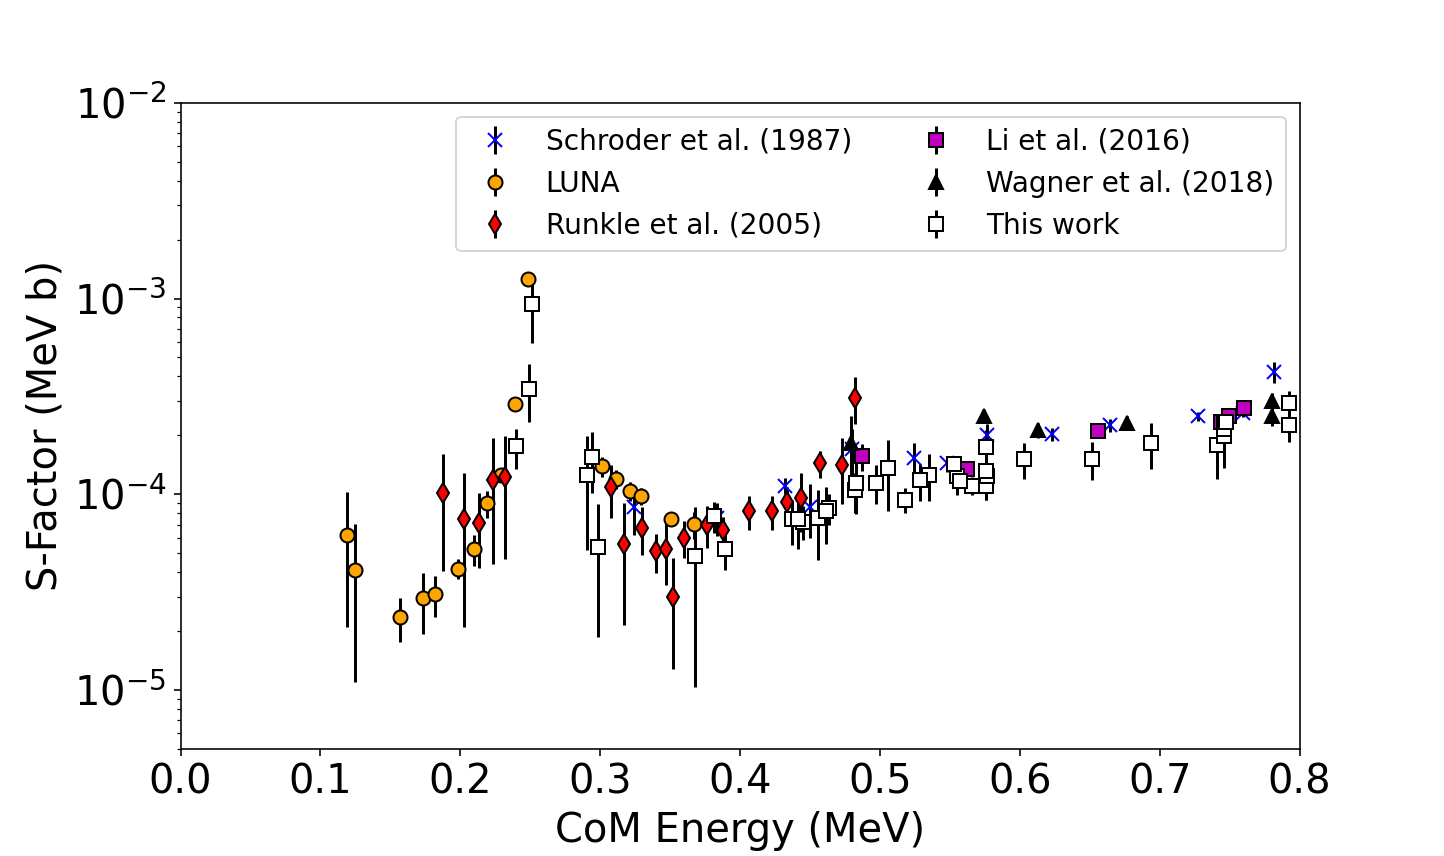
\includegraphics[width=1.0\linewidth]{figures/low_mid_gs.png}
	\caption{Differential cross section for the ground state transition in the $^{14}$N$\left( p,\gamma \right) ^{15}$O reaction, primarily detailing the off resonance region measured at CASPAR in this experiment. Also plotted are data from \cite{Schroder1987, Imbriani2005, Runkle2005, Li2016} for comparison. The LUNA data specifically represents the measurements \cite{Formicola2004, Imbriani2005, Marta2008, Marta2011}. Our data and that from \citet{Li2016} were both calculated as differential $S$-factors but scaled up by a factor of $4\pi$ for plotting purposes.    }
	\label{fig: midGS}
\end{figure}



\begin{figure}
\thisfloatpagestyle{plain}
		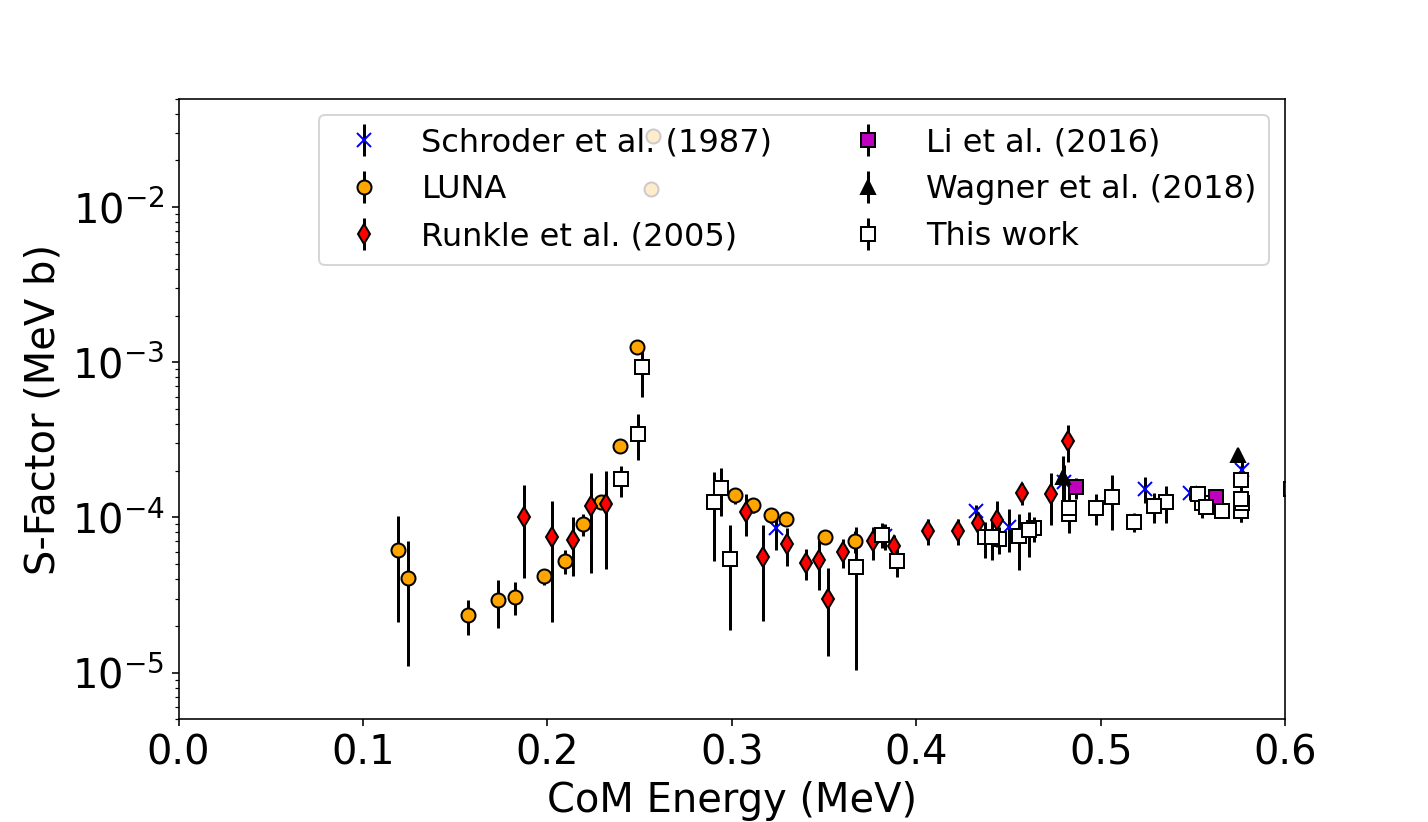
\includegraphics[width=1.0\linewidth]{figures/low_gs.png}
	\caption{Differential cross section for the ground state transition in the $^{14}$N$\left( p,\gamma \right) ^{15}$O reaction, showing the behavior of the $S$-factor at low energy. Also plotted are data from \cite{Schroder1987, Imbriani2005, Runkle2005, Li2016} for comparison. The LUNA data specifically represents the measurements \cite{Formicola2004, Imbriani2005, Marta2008, Marta2011}. Our data and that from \citet{Li2016} were both calculated as differential $S$-factors but scaled up by a factor of $4\pi$ for plotting purposes. }
	\label{fig: lowGS}
\end{figure}

%\begin{figure}
%\thisfloatpagestyle{plain}
%		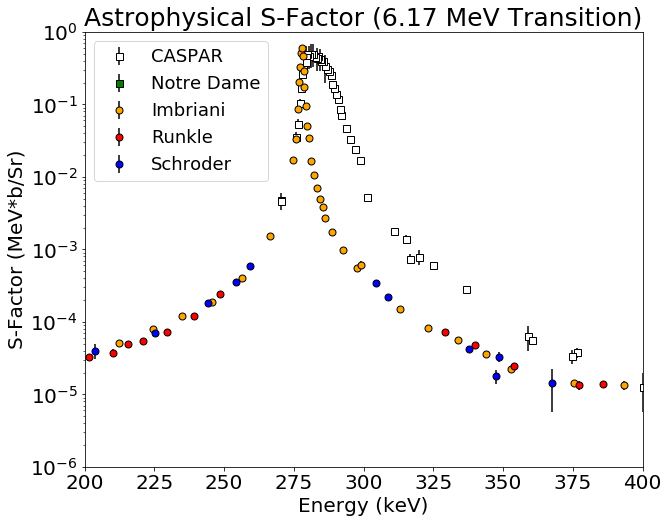
\includegraphics[width=1.0\linewidth]{figures/low617.png}
%	\caption{Differential cross section for the 6.17 MeV transition in the $^{14}$N$\left( p,\gamma \right) ^{15}$O reaction, showing the behavior of the $S$-factor at low energy. Also plotted are data from \cite{Schroder1987, Imbriani2005, Runkle2005, Li2016} for comparison. }
%	\label{fig: low617}
%\end{figure}

% % uncomment the following lines,
% if using chapter-wise bibliography
%
% \bibliographystyle{ndnatbib}
% \bibliography{example}


%
% Chapter 4
%

%
% Modified by Megan Patnott
% Last Change: Jan 18, 2013
%
%%%%%%%%%%%%%%%%%%%%%%%%%%%%%%%%%%%%%%%%%%%%%%%%%%%%%%%%%%%%%%%%%%%%%%%%
%
% Modified by Sameer Vijay
% Last Change: Tue Jul 26 2005 13:00 CEST
%
%%%%%%%%%%%%%%%%%%%%%%%%%%%%%%%%%%%%%%%%%%%%%%%%%%%%%%%%%%%%%%%%%%%%%%%%
%
% Sample Notre Dame Thesis/Dissertation
% Using Donald Peterson's ndthesis classfile
%
% Written by Jeff Squyres and Don Peterson
%
% Provided by the Information Technology Committee of
%   the Graduate Student Union
%   http://www.gsu.nd.edu/
%
% Nothing in this document is serious except the format.  :-)
%
% If you have any suggestions, comments, questions, please send e-mail
% to: ndthesis@gsu.nd.edu
%
%%%%%%%%%%%%%%%%%%%%%%%%%%%%%%%%%%%%%%%%%%%%%%%%%%%%%%%%%%%%%%%%%%%%%%%%


%
% Chapter 4
%


\chapter{Lifetime Measurements}
\label{chap: lifetime}

This chapter presents the details of the analysis used for the determination of the lifetime of the 6.79 MeV state, the 5.18 MeV state, and the 6.17 MeV state in $^{15}$O. These data resulted from a nine-day long experiment at the university of Notre Dame Nuclear Science Laboratory in August 2019. This measurement used protons from the 5U Sta. Ana accelerator for the $^{14}$N(p,$\gamma$)$^{15}$O reaction at beam energies ranging from 1 MeV to 1.6 MeV. Further description of this experimental setup, targets, and methodology can be found in Chapter \ref{chap: experiment}.	

\section{Determining a nuclear lifetime}
\label{sec: lifetime determination}

For this analysis, a new DSAM program was written to simulate the expected Doppler shift and lineshape. This approach, as will be outlined shortly, follows the Monte Carlo (MC) technique for simulating physical phenomena with the sampling of random numbers. A full reproduction of the code is provided for reference in Appendix \ref{appendix: codes}. 

The MC technique is simple enough in idea and a powerful tool across the fields of physics and mathematics: to numerically estimate phenomena by studying their effects with reasonably sampled, random numbers. In other words, the aim is to build a probability distribution that is proportional to some function, $P(x)$, which spans the interval $[x_{min}, x_{max}]$, using random numbers in the range [0,1]. To start, take the integral of the function over some subset of its total range,

\begin{equation}
I(x) = \int_{x_{min}}^{x} P(x') dx',
\label{eqn: mcStart}
\end{equation}

\noindent where $x_{min} \leq x \leq x_{max}$. Normalizing this integral to the integral over the complete range,

\begin{equation}
I_{norm}(x) = \dfrac{I(x)}{I(x_{max})} = \dfrac{\int_{x_{min}}^{x} P(x') dx'}{\int_{x_{min}}^{x_{max}} P(x') dx'},
\end{equation}

\noindent creates the desired relationship, since the integrated probability is itself a random variable and the normalization guarantees its range is confined to [0, 1]. This is shown when evaluating $I_{norm}$ at the extremes of its domain,

\begin{equation}
I_{norm} (x_{min}) = \dfrac{\int_{x_{min}}^{x_{min}} P(x') dx'}{\int_{x_{min}}^{x_{max}} P(x') dx'} = 0
\end{equation}

\noindent and

\begin{equation}
I_{norm} (x_{max}) = \dfrac{\int_{x_{min}}^{x_{max}} P(x') dx'}{\int_{x_{min}}^{x_{max}} P(x') dx'} = 1.
\end{equation}

\noindent Finally, then, to utilize this relationship in the MC technique, $I_{norm}$ is evaluated for a specific function and ultimately inverted to produce a response in the original function, $P(x)$, as a function of a randomly generated number in the range of [0, 1].

Specifically, the case of interest in this work involves the modeling of exponential decay,

\begin{equation}
P(x) = e^{-\lambda x},
\end{equation}

\noindent where $\lambda$ is the width and inversely proportional to the lifetime, $\lambda = 1/ \tau$. In this context, the domain of input variable, $x$, is [0, $\infty$], as the decay can occur at any time. Utilizing this in the formulation starting with Equation \ref{eqn: mcStart},

\begin{equation}
I(x) = \int_{0}^{x} e^{-\lambda x'} dx' = \frac{1}{\lambda} (1 - e^{-\lambda x}),
\end{equation}

\begin{equation}
I(x_{min}) = I(0) = 0,
\end{equation}

\begin{equation}
I(x_{max}) = I(\infty) = 1/\lambda,
\end{equation}

\noindent and, ultimately, 

\begin{equation}
I_{norm}(x) = \frac{\lambda^{-1}(1 - e^{-\lambda x})}{\lambda^{-1}} = (1 - e^{-\lambda x}).
\label{eqn: exponentialGenerator}
\end{equation}

\noindent An example of this approach is plotted for reference in Fig.\ \ref{fig: expoGen}. This plots Equation \ref{eqn: exponentialGenerator} for the arbitrary choice of $\lambda$=50 to demonstrate the operational principles. The range of this function's response is limited to [0, 1], as it approaches 1 asymptotically. While the input variable, decay time, is only plotted to 0.1 in this figure, the behavior does not change at higher values and was only chosen to highlight this method. Now, a random number, $r$, can be generated on the range [0, 1], i.e.\ within the range of $I_{norm}(x)$, and this curve can be used to look up and identify a value for the specific decay time, $x$. 



\begin{figure}
\thisfloatpagestyle{plain}
\centering
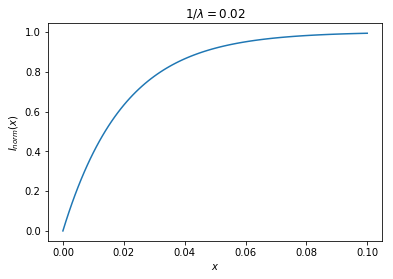
\includegraphics[width=0.85\linewidth]{figures/expoDecayGenerator.png}
\caption{An example of the Monte Carlo method for constructing a relationship between a function and the random number generator. This plots the $I_{norm}(x)$ of Equation \ref{eqn: exponentialGenerator} for an arbitrary choice of $\lambda = 50$ to demonstrate the technique. The range of the response of this function is limited to [0, 1] asymptotically, while the input variable of decay time is unrestricted. }
\label{fig: expoGen}
\end{figure}


However, this can be more instructive to invert the function and create a relationship to output a decay time for a randomly generated $r$ and a given width and lifetime, $\lambda$ and $\tau$, respectively.  This is done as,

\begin{equation}
r = 1 - e^{-\lambda x} \Rightarrow e^{\lambda x} = \dfrac{1}{1-r} \Rightarrow x = \dfrac{1}{\lambda} \ln \left( \frac{1}{1-r} \right).
\label{eqn: rand}
\end{equation}

\noindent The above relationship is then used to simulate a decaying nucleus. By selecting a random number within [0, 1] one can determine the corresponding decay time of a nucleus with a given lifetime from Equation \ref{eqn: rand}. For a large amount of randomly generated numbers, the general behavior of the initial function, exponential decay in this case, can be simulated and studied. An example of this is shown in Fig.\ \ref{fig: simExample} for 100,000 such events. The total behavior can be stored and compared with the original decay law. To do this, however, the simulated histogram must be normalized to match the properties of the original function, $P(x)$.  Namely, the survival cannot be greater than 1, and, indeed, $P(0) = 1$. Therefore, by normalizing the whole histogram to the value of the first histogram bin, the simulated decay curve can be compared to the function from which it was generated. As Fig.\ \ref{fig: simCompare} demonstrates, this is a effective and faithful method of simulating these natural phenomena. 


\begin{figure}
\centering
\includegraphics[width=0.85\linewidth]{figures/simExample.png}
\caption{An example of the Monte Carlo method for a simulated decay curve. For 100,000 simulated nuclear decays with a $\lambda$=50, the MC method generates the given histogram of decay times.  }
\label{fig: simExample}
\end{figure}


\begin{figure}
\thisfloatpagestyle{plain}
\centering
\includegraphics[width=\linewidth]{figures/simCompareExample.png}
\caption{An example of the Monte Carlo method for a simulated decay curve. For 100,000 simulated nuclear decays with a $\lambda$=50, the MC method generates the given histogram of decay times.  }
\label{fig: simCompare}
\end{figure}


It is upon these principles and this derived formulation that the experimentally measured nuclear lifetimes were extracted. A full reproduction of the code is provided for reference in Appendix \ref{appendix: codes}. The important components of the code are illustrated in Fig.\ \ref{fig: simSteps} and the logic of the code is as follows:


\begin{figure}
\thisfloatpagestyle{plain}
\centering
\includegraphics[width=\linewidth]{figures/simSteps.pdf}
\caption{The major steps of the Monte Carlo DSAM simulation for each $\gamma$ ray event. The details of the process are provided in the text, with a complete reproduction of the code also included in Appendix \ref{appendix: codes}.}
\label{fig: simSteps}
\end{figure}


\begin{enumerate}
\item First, recoil ion travel paths were calculated with the SRIM software \cite{Ziegler2010} (another Monte Carlo simulation) for each target material, accounting for the nitrogen present. For this, the reaction recoil energy was calculated and used as the input energy of the ion. The initial energy was randomly assigned to a reasonable range based on the energy loss in the target before reaching the implanted depth of nitrogen. All recoils were assumed to have initial velocity parallel to the incident beam axis. Then, the software calculates the path of the ions travel, recording the the ion's energy, the location of each collision, and the stopping power felt at that position. These tracks are randomly generated for 10,000 different ions. The standard SRIM output is sufficient in this case as the energy regime for this reaction is not high enough to warrant relativistic corrections, like the methods of \cite{Galinski2014, Michelagnoli2013}. 
\item Next, based on the information from the SRIM output, further information about each ion's travel is calculated. Specifically, utilizing the position of each interaction, the particle's trajectory is calculated between each collision. Using the ion's energy at each point, the speed is calculated. Then, ultimately using these data, the time for each interaction (in femtoseconds) is determined. This provides a complete picture of any single ion's calculated motion through the target material. As these are not relativistic quantities, standard freshman kinematics relations are all that is necessary to calculate this information.
\item Of the 10,000 tracks for which the information has been calculated, randomly select one to be the specific decaying ion's path. 
\item Choose a specific nuclear lifetime for the decaying nuclear state to simulate and angle of detection. The angles chosen to simulate were the same as the angles used in the measurement for a direct comparison. 
\item Using the relationship in Equation \ref{eqn: rand} and the specified nuclear lifetime from the previous step, randomly generate a decay time for the recoiling nucleus.  
\item At the given, generated decay time, the code looks up the calculated information for the previous and subsequent collisions. From these, it interpolates between the two interactions to find the position and velocity of the decaying nucleus. 
\item Calculate, explicitly, the Doppler shifted energy, $E_{\gamma}$, from a nucleus decaying at this time, with a specified velocity, $\beta = v/c$, and with the gamma being observed by a detector at a specified angle, $\theta$,

\begin{equation}
E_{\gamma} = E_{\gamma}^{0} ( 1 + \beta \cos (\theta)) \times R
\label{eqn: doppSim}
\end{equation}

\noindent where $R$ represents a correction to account for the detector size and resolution, determined from the experimental spectra, and $E_{\gamma}^{0}$ is the unshifted $\gamma$ ray energy. At this point, it is important to note that as this measurement was not intended to calculate a cross-section, the detection efficiency is not included in this simulation. 
\item The code then records the energy of this measured $\gamma$-ray and adds it to a histogram for it's specific decay time, measured angle, and target material. This behavior is illustrated in Fig.\ \ref{fig: simulatedSingle}, which shows the simulated energy deposition histograms at each of the angles.

\begin{figure}
\thisfloatpagestyle{plain}
\centering
\includegraphics[width=\linewidth]{figures/simulatedSingle.png}
\caption{Simulated energy deposition histograms for the Mo target implantation material with a nuclear lifetime of $\tau=0.5$ fs from the decay of the 6792 keV state in $^{15}$O. Each histogram represents the detection of the 50,000 of the decaying $\gamma$-rays at the angle specified. As all the histograms share common axis bounds, the Doppler shift with angle can clearly be seen. The plot for 0 degree shows the maximum shifted gamma ray, where the unshifted photons arrive at 6792 keV in the 90 degree histogram, matching the real data. A plot of all shifts together is shown later, in Fig.\ \ref{fig: simulatedAll}. The shifting down of the peak with respect to angle shows the Doppler Shift in action.}
\label{fig: simulatedSingle}
\end{figure}

\item The code then returns to Step 3 and repeats this simulation for 50,000 decays for each detection angle, lifetime, and target material combination. An even clearer example of the Doppler shift within this MC simulation is presented in Fig.\ \ref{fig: simulatedAll}. This presents one specific lifetime, $\tau=0.5$ fs, with the Mo backing to show all the simulated $\gamma$'s on one plot. This shows the boost in energy at forward angles ($\theta < 90 \degree$) and the reduction in energy at backward angles ($\theta > 90 \degree$). 


\begin{figure}
\thisfloatpagestyle{plain}
\centering
\includegraphics[width=\linewidth]{figures/simAllAngles.png}
\caption{Simulated energy deposition histogram for all detection angles. This plot was produced from the decay of $^{15}$O through the 6.79 MeV state with the Mo backing material and lifetime $\tau=0.5$ fs, where each color represents a different detection angle. Clearly illustrated in this figure is the Doppler shift of the $\gamma$ ray energies with changing angle, the relationship upon which the entire DSA method is predicated. After each peak in this figure is fit with a Gaussian, the centroids were used to determine the energy shift as a function of angle. Under these simulated conditions, the maximum shift is roughly 26 keV. The unshifted photons are also detected at 6792 keV, exactly matching experimental conditions.}
\label{fig: simulatedAll}
\end{figure}


\item These aggregate histograms are all used to determine the peak locations since they are the shifted peaks. This establishes the direct link between the gamma's energy and angle. Therefore, the relationship between shifted $\gamma$ ray energy at each of the conditions for lifetime, angle, and material is determined in this way. 
\item At this point, takes all of this information from each combination to plot a relationship between the observed energy in the detector vs. $\cos(\theta)$, as is done in the experiment. Each is fit with a line, the slope of which contains the attenuation factor information. An example of this process is illustrated in Fig.\ \ref{fig: simSlopes}, showing all of the combinations of lifetime and angle for the Mo target simulations.

\begin{landscape}
\begin{figure}
\thisfloatpagestyle{plain}
\centering
\includegraphics[width=0.7\linewidth]{figures/simSlopes.png}
\caption{Determining the relationship between shifted peak energy and $\cos(\theta)$ for all simulated Mo lifetime combinations. This provides the output of the slopes for each simulated condition, allowing one to establish a relationship between the slopes and the attenuation factor. More details are provided in the text. }
\label{fig: simSlopes}
\end{figure}
\end{landscape}

These slopes are then normalized to the slope for a maximally shifted distribution, which is calculated from the reaction parameters. This normalized slope value is the attenuation factor, which can be experimentally determined. With this then, a relationship has been fabricated between the attenuation factor, $F(\tau)$, and the nuclear lifetime, $\tau$. An example of this relationship is shown in Fig.\ \ref{fig: attFacExample}. 
\item With the experimentally determined attenuation factors and uncertainties, the code calculates the corresponding lifetime and uncertainties, allowing one to ultimately determine the lifetime of an experimentally measured Doppler shift. 
\end{enumerate}

\begin{figure}
\thisfloatpagestyle{plain}
\centering
\includegraphics[width=\linewidth]{figures/attFacExample.png}
\caption{The calculated attenuation factors, $F(\tau)$, for the various experimental backings, as a function of the nuclear lifetime, $\tau$. This example of their relationship shows the various targets used in the measurement  and the response in the range of very short lifetimes, $\tau < 5$ fs, for the 6.79 MeV state in $^{15}$O. }
\label{fig: attFacExample}
\end{figure}



\section{Systematic errors and uncertainties}
\label{sec: systematicErrors}

This section details the instances and sources of systematic errors and uncertainties that arose in this treatment of the data and how they were managed.

\begin{enumerate}
\item In describing the SRIM software, Ziegler \textit{et al}.\ quoted the uncertainties in the programs stopping powers as 5\% \cite{Ziegler2010}. This was propagated through to an uncertainty in the initial energy of the recoiling ion paths as generated by SRIM for use in the MC simulation. This, ultimately, manifests in the distributions of $\gamma$ ray energies produced in the simulation and does not need to be otherwise included explicitly in this calculation. 
\item A significant difference between this procedure and other, previous methods for calculating the lifetimes is that this is not an analytical expression of the parameters and is only a numerical calculation. As a matter of fact, this is only a discrete calculation at values chosen across the relevant lifetime landscape. Therefore, these attenuation factors require an external fit to provide the final relationship. To minimize any artificial bias from the choice of simulated lifetimes, the lifetimes were chosen to range across the entire expected range of values and beyond to ensure that the relationship is robust in the relevant lifetime ranges. 
\item When considering the nominal angles of the detector placement in the measurement, it is critical that these be accurate to the target or they will introduce artificial changes in the Doppler shift relation. Put another way, if the target is not located at the axis of rotation for the detector, there will be an additional difference in the angles, causing inaccurate $F(\tau)$ determinations. To ensure that the target is at the axis of rotation for the detector, spectra were obtained at $\pm$ 90$\degree$. At both angles, $E_{\gamma}$ should be unshifted, since this angle is perpendicular to the motion of the recoiling nuclei. Therefore, the spectra at these angles should, and do, lie exactly on top of each other. This is presented in Fig.\ \ref{fig: pm90}. The agreement of these spectra demonstrates that the target was located at the center of the measurement apparatus and guarantees that the measured angles are accurate.

\begin{figure}
\thisfloatpagestyle{plain}
\centering
\includegraphics[width=\linewidth]{figures/pm90comparison.pdf}
\caption{Measured energy spectrum of the 6.79 MeV transition at $\pm$90$\degree$. At these two angles, the energy of the $\gamma$ ray is not Doppler shifted and so the fact that both spectra show perfect agreement indicates that there is no systematic effect in our measurement from inaccurate angular determination of the detector's positions.}
\label{fig: pm90}
\end{figure}


\item In fitting the peaks present in the spectra, the centroid, area, and width are extracted after removing a linear background contribution from the spectrum. The background was fit separately from the peak using regions surrounding the peak of interest to increase the fidelity of the background estimation. Fig.\ \ref{fig: bgfit} demonstrates this procedure. In this high-energy region of the spectrum, a linear background is a reasonable assumption, as the background always is quite small and peaks are typically well isolated from each other. 

\begin{figure}
\thisfloatpagestyle{plain}
\centering
\includegraphics[width=0.7\linewidth]{figures/bgFit.pdf}
\caption{The stopped $\gamma$ ray peak as an example of the background subtraction method. The regions surrounding the peak of interest (marked by the black, vertical lines) are fit with a linear term to describe the background underneath the peak, which is fit separately with a Gaussian. }
\label{fig: bgfit}
\end{figure}

\item Due to experimental time constraints, the low dose implanted Ta target was only measured with two angles. Since two points define a line completely, the data give no measure of uncertainty. Therefore, this was ultimately excluded from subsequent analysis.
\item Compared to the cross section measurements, the number of $^{14}$N($p,\gamma)^{15}$O reactions that occur is not necessary for the lifetime determination, only the shift of the gamma's peak in the spectrum. As such, correcting the spectrum for efficiency or dead-time are unnecessary, as both effects only adjust the number of counts in a spectrum. Particularly when considering a small range of energies (like the 20 keV under a peak), efficiency effects are consistent across the peak range. Similarly, as dead-time effects are not energy dependent, they do not introduce any mis-shaping or artificial shifting of the peak.
%\item Orthogonal distance relation
\item The measurement uncertainties in the angle and centroid energy of the $\gamma$ peaks are represented as X and Y uncertainties, respectively, in evaluating the Doppler shift as function of angle. These are then propagated through a fit of the slope as the uncertainty on that fit parameter. As traditional least-squares fitting relies only on uncertainty in the Y position of data, these were fit with a method called Orthogonal Distance Regression (ODR), which incorporates point uncertainties in both the X and Y directions for the fit. Therefore, the slopes and uncertainties extracted by this ODR method have a higher fidelity compared with the traditional least-squares method. 
\end{enumerate}

\section{Lifetime of the 5.18 MeV state in $^{15}$O}
\label{sec: lifetime518}

The experimental Doppler shift of the $\gamma$ ray peaks for this decay can be seen in Fig.\ \ref{fig: shift518}. This figure displays the spectra for all of the measurements with different target materials and plots the spectra of different angular measurements together. This figure directly shows the shifting $\gamma$ ray peak for each of the angles measured in this work. Each of these were then fit with a Gaussian and underlying linear background, as described in Sec.\ \ref{sec: systematicErrors}, to determine their centroid and uncertainty. 


\begin{figure}
\thisfloatpagestyle{plain}
\centering
\includegraphics[width=0.6\linewidth]{figures/shifts518.png}
\caption{The Doppler shifted spectra taken during this measurement for the 5.18 MeV state. a) shows the spectra from the Mo implanted target, b) depicts the spectra from the Ta implanted target, and c) gives the spectra from the W implanted target.Within these, the Doppler shift boosting the energy of the $\gamma$ ray peak  with a change in angle can be clearly seen. }
\label{fig: shift518}
\end{figure}


With the measured energies of the $\gamma$-rays and their uncertainties, the relationship between the cosine of the measurement angle, $\cos(\theta)$, and the observed energies, $E_{\gamma}$, were determined for each of the target materials. This was achieved by fitting a straight line to the data with ODR, accounting for uncertainties in X and Y. Recall, the slope of this line is related to the experimentally measured attenuation factor, $F(\tau)$, which contains the lifetime information. These relationships are plotted in Fig.\ \ref{fig: doppler518} and their corresponding extracted $F(\tau)$ values are provided in Table \ref{table: afTau518}. The attenuation factor for this state with the Mo implanted target was $F(\tau)_{\text{Mo}} = 0.904 \pm 0.013$, $F(\tau)_{\text{Ta}} = 0.911 \pm 0.016$ with the Ta implanted target, and $F(\tau)_{\text{W}} = 0.912 \pm 0.015$ with the W implanted targets.


\begin{figure}
\thisfloatpagestyle{plain}
\centering
\includegraphics[width=\linewidth]{figures/doppler518.png}
\caption{The relationship between the measured angle, $\cos(\theta)$, and the measured $\gamma$ peak energy, $E_{\gamma}$ of the 5.18 MeV state for the a) Mo target, b) Ta target, and c) W target. The slopes, which contain the information about the attenuation factor, $F(\tau)$, and ultimately the lifetime, $\tau$, were determined with Orthogonal Distance Regression (see text for details). }
\label{fig: doppler518}
\end{figure}


\begin{table}[]
\thisfloatpagestyle{plain}
\caption{ATTENUATION FACTORS AND LIFETIMES OF THE 5.18 MeV STATE MEASURED IN THIS WORK}
\centering
\begin{threeparttable}
\begin{tabular}{@{}lllll@{}}
\toprule
                   & Mo Target  & Ta Target & W Target & Weighted Average \\ \midrule
$F(\tau)_{5.18}$   & $9.040 \pm 0.013$     & $0.911 \pm 0.016$   & $9.120 \pm 0.015$   &                  \\
$\tau_{5.18}$ (fs) & $7.1^{+4.8}_{-2.3}$ & $7.1 \pm 5.5$       & $8.0 \pm 6.7$      & $7.3 \pm 3.2$    \\ \bottomrule
\end{tabular}
\begin{tablenotes}
\small 
\item A summary of the attenuation factors and lifetime measurements for the 5.18 MeV state in $\ce{^{15}O}$. All measurements are listed with their corresponding target material and the weighed average for the lifetime is also provided. To note, it is not possible to take a weighted average of the attenuation factor because the response of the attenuation factor to lifetime is highly dependent on the target material, so only an average of the extracted lifetimes are accurate.
\end{tablenotes}
\end{threeparttable}
\label{table: afTau518}
\end{table}

For this state, the attenuation factor curves, which relates the nuclear lifetime to the $F(\tau)$ values, are shown for each target material in Fig.\ \ref{fig: attFacs518}. It is through this relationship that the measured lifetimes are determined. From the measured attenuation factors, the measured lifetimes for this state are $\tau_{\text{Mo}} = 7.1^{+4.8}_{-2.3}$ fs with the Mo implanted target, $\tau_{\text{Ta}} = 7.1 \pm 5.5$ fs with the Ta implanted target, and $\tau_{\text{W}} = 8.0 \pm 6.7$ fs from the W implanted target. The weighted average of these measurements is $\overline{\tau} = 7.3 \pm 3.2$ fs. These values, as well as existing literature measurements of the lifetime of this state, are presented in Fig.\ \ref{fig: lifetimes518} and are summarized in Table \ref{table: afTau518}. As can be seen, these new measurements have significantly higher uncertainties than previous measurements of this state's lifetime. This large uncertainty arises in part from the double escape peak at $E_{\gamma} = 5150$ keV (from the $E_{\gamma} = 6172$ keV full energy peak) that complicates the background determination (and therefore the peak centroids for the Doppler Shift). This, taken in combination with the flat response of the attenuation factor to lifetime in this range (as can be seen in Fig.\ \ref{fig: attFacs518}) makes for a less certain determination of the lifetime. Due to this, even a small error of 1-2\% in the $F(\tau)$ compounds into a larger uncertainty in the measured lifetime. Ultimately, this means that we have a less precise value than those of Refs.\ \cite{Bertone2001, Schurmann2008, Gill1968} but we still show good agreement with all three of those reported values.


\begin{figure}
\thisfloatpagestyle{plain}
\centering
\includegraphics[width=\linewidth]{figures/attFac518.png}
\caption{The calculated attenuation factors, $F(\tau)$, for the various experimental backings, as a function of the nuclear lifetime, $\tau$, for the 5.18 MeV state in $^{15}$O. While the low dose Ta target is included in the calculation, it was excluded for a lifetime determination (see Section \ref{sec: systematicErrors} for details). }
\label{fig: attFacs518}
\end{figure}


\begin{figure}
\thisfloatpagestyle{plain}
\centering
\includegraphics[width=\linewidth]{figures/lifetimes518.png}
\caption{Measured lifetimes and the weighted average lifetime of the 5.18 MeV state in $^{15}$O determined in this work alongside literature values. The TUNL measurement is Ref.\ \cite{Bertone2001} and the Bochum measurement is Ref.\ \cite{Schurmann2008}. On the whole, our measured values are less precise than the other literature values, but agree well with those same reports. Our measurements for this state were made less precise because the peak was on the shoulder of another, making the centroid determination more uncertain.}
\label{fig: lifetimes518}
\end{figure}



\section{Lifetime of the 6.17 MeV state in $^{15}$O}
\label{sec: lifetime617}


The experimental Doppler shift of the $\gamma$ ray peaks for this decay can be seen in Fig.\ \ref{fig: shift617}. This figure displays the spectra for all of the measurements with different target materials and plots the spectra of different angular measurements together. This figure directly shows the shifting $\gamma$ ray peak for each of the angles measured in this work. Each of these were then fit with a Gaussian and underlying linear background, as described in Sec.\ \ref{sec: systematicErrors}, to determine their centroid and uncertainty. 


\begin{figure}
\thisfloatpagestyle{plain}
\centering
\includegraphics[width=0.6\linewidth]{figures/shifts617.png}
\caption{The Doppler shifted spectra taken during this measurement for the 6.17 MeV state. a) shows the spectra from the Mo implanted target, b) depicts the spectra from the Ta implanted target, and c) gives the spectra from the W implanted target.Within these, the Doppler shift boosting the energy of the $\gamma$ ray peak  with a change in angle can be clearly seen. }
\label{fig: shift617}
\end{figure}


With the measured energies of the $\gamma$-rays and their uncertainties, the relationship between the cosine of the measurement angle, $\cos(\theta)$, and the observed energies, $E_{\gamma}$, were determined for each of the target materials. This was achieved by fitting a straight line to the data with ODR, accounting for uncertainties in X and Y. Recall, the slope of this line is related to the experimentally measured attenuation factor, $F(\tau)$, which contains the lifetime information. These relationships are plotted in Fig.\ \ref{fig: doppler617} and their corresponding extracted $F(\tau)$ values are provided in Table \ref{table: afTau617}. The attenuation factor for this state with the Mo implanted target was $F(\tau)_{\text{Mo}} = 0.992 \pm 0.014$, $F(\tau)_{\text{Ta}} = 0.976 \pm 0.017$ with the Ta implanted target, and $F(\tau)_{\text{W}} = 0.988 \pm 0.016$ with the W implanted targets.


\begin{figure}
\thisfloatpagestyle{plain}
\centering
\includegraphics[width=\linewidth]{figures/doppler617.png}
\caption{The relationship between the measured angle, $\cos(\theta)$, and the measured $\gamma$ peak energy, $E_{\gamma}$ of the 6.17 MeV state for the a) Mo target, b) Ta target, and c) W target. The slopes, which contain the information about the attenuation factor, $F(\tau)$, and ultimately the lifetime, $\tau$, were determined with Orthogonal Distance Regression (see text for details). }
\label{fig: doppler617}
\end{figure}

\begin{table}[]
\thisfloatpagestyle{plain}
\caption{ATTENUATION FACTORS AND LIFETIMES OF THE 6.17 MeV STATE MEASURED IN THIS WORK}
\centering
\begin{threeparttable}
\begin{tabular}{@{}lllll@{}}
\toprule
                   & Mo Target & Ta Target & W Target  & Weighted Average \\ \midrule
$F(\tau)_{6.17}$   & $0.992 \pm 0.014$   & $0.976 \pm 0.017$   & $0.988 \pm 0.016$   &                  \\
$\tau_{6.17}$ (fs) & $0.4^{+0.7}_{-0.4}$ & $1.4 \pm 1.0$       & $0.6^{+0.9}_{-0.6}$ & $0.7 \pm 0.5$    \\ \bottomrule
\end{tabular}
\begin{tablenotes}
\small 
\item A summary of the attenuation factor and lifetime measurements for the 6.17 MeV state in $\ce{^{15}O}$. All measurements are listed with their corresponding target material and their weighed average is provided. To note, it is not possible to take a weighted average of the attenuation factor because the response of the attenuation factor to lifetime is highly dependent on the target material, so only an average of the extracted lifetimes are accurate.
\end{tablenotes}
\end{threeparttable}
\label{table: afTau617}
\end{table}

For this state, the attenuation factor curves, which relates the nuclear lifetime to the $F(\tau)$ values, are shown for each target material in Fig.\ \ref{fig: attFacs617}. It is through this relationship that the measured lifetimes are determined. From the measured attenuation factors, the measured lifetimes for this state are $\tau_{\text{Mo}} = 0.4^{+0.7}_{-0.4}$ fs with the Mo implanted target, $\tau_{\text{Ta}} = 1.4 \pm 1.0$ fs with the Ta implanted target, and $\tau_{\text{W}} = 0.6^{+0.9}_{-0.6}$ fs from the W implanted target. The weighted average of these measurements is $\overline{\tau} = 0.7 \pm 0.5$ fs. These values, as well as existing literature measurements of the lifetime of this state, are presented in Fig.\ \ref{fig: lifetimes617} and are summarized in Table \ref{table: afTau617}. For this state, we report a significantly more precise value than those of Refs.\ \cite{Bertone2001, Schurmann2008, Galinski2014}. We show only a minimal agreement within uncertainty to the TUNL measurement \cite{Bertone2001}. Our reported value is engulfed entirely within the upper bound placed by \cite{Galinski2014} and lies just within the edge of the upper bound reported in \cite{Schurmann2008}, with a significant overlap on our uncertainty range. Our value, thus, aligns most agreeably with that of Sch{\"u}rmann \textit{et al.} \cite{Schurmann2008}.


\begin{figure}
\thisfloatpagestyle{plain}
\centering
\includegraphics[width=\linewidth]{figures/attFac617.png}
\caption{The calculated attenuation factors, $F(\tau)$, for the various experimental backings, as a function of the nuclear lifetime, $\tau$, for the 6.17 MeV state in $^{15}$O. While the low dose Ta target is included in the calculation, it was excluded for a lifetime determination (see Section \ref{sec: systematicErrors} for details).}
\label{fig: attFacs617}
\end{figure}


\begin{figure}
\thisfloatpagestyle{plain}
\centering
\includegraphics[width=\linewidth]{figures/lifetimes617.png}
\caption{Measured lifetimes and the weighted average lifetime of the 5.18 MeV state in $^{15}$O determined in this work alongside literature values. The TUNL measurement is Ref.\ \cite{Bertone2001}, the Bochum measurement is Ref.\ \cite{Schurmann2008}, and the TRIUMF measurement is Ref.\ \cite{Galinski2014}. Here, our results are more precise and agree very well with the measurements of Sch{\"u}rmann \textit{et al.} \cite{Schurmann2008} and Galinski \textit{et al.} \cite{Galinski2014}, while also showing weak agreement with the measurement reported by Ref.\ \cite{Bertone2001}. The measurements reported by \citet{Schurmann2008} and \citet{Galinski2014} are only upper limits, so they are represented only as that bound in this figure.}
\label{fig: lifetimes617}
\end{figure}



\section{Lifetime of the 6.79 MeV state in $^{15}$O}
\label{sec: lifetime679}


The experimental Doppler shift of the $\gamma$ ray peaks for this decay can be seen in Fig.\ \ref{fig: shift679}. This figure displays the spectra for all of the measurements with different target materials and plots the spectra of different angular measurements together. This figure directly shows the shifting $\gamma$ ray peak for each of the angles measured in this work. Each of these were then fit with a Gaussian and underlying linear background, as described in Sec.\ \ref{sec: systematicErrors}, to determine their centroid and uncertainty. 


\begin{figure}
\thisfloatpagestyle{plain}
\centering
\includegraphics[width=0.6\linewidth]{figures/shifts679.png}
\caption{The Doppler shifted spectra taken during this measurement for the 6.79 MeV state. a) shows the spectra from the Mo implanted target, b) depicts the spectra from the Ta implanted target, and c) gives the spectra from the W implanted target.Within these, the Doppler shift boosting the energy of the $\gamma$ ray peak  with a change in angle can be clearly seen. }
\label{fig: shift679}
\end{figure}


With the measured energies of the $\gamma$-rays and their uncertainties, the relationship between the cosine of the measurement angle, $\cos(\theta)$, and the observed energies, $E_{\gamma}$, were determined for each of the target materials. This was achieved by fitting a straight line to the data with ODR, accounting for uncertainties in X and Y. Recall, the slope of this line is related to the experimentally measured attenuation factor, $F(\tau)$, which contains the lifetime information. These relationships are plotted in Fig.\ \ref{fig: doppler679} and their corresponding extracted $F(\tau)$ values are provided in Table \ref{table: afTau679}. The attenuation factor for this state with the Mo implanted target was $F(\tau)_{\text{Mo}} =0.995 \pm 0.019$, $F(\tau)_{\text{Ta}} = 0.983 \pm 0.019$ with the Ta implanted target, and $F(\tau)_{\text{W}} = 0.978 \pm 0.015$ with the W implanted targets.


\begin{figure}
\thisfloatpagestyle{plain}
\centering
\includegraphics[width=\linewidth]{figures/doppler679.png}
\caption{The relationship between the measured angle, $\cos(\theta)$, and the measured $\gamma$ peak energy, $E_{\gamma}$ of the 6.79 MeV state for the a) Mo target, b) Ta target, and c) W target. The slopes, which contain the information about the attenuation factor, $F(\tau)$, and ultimately the lifetime, $\tau$, were determined with Orthogonal Distance Regression (see text for details). }
\label{fig: doppler679}
\end{figure}

\begin{table}[]
\thisfloatpagestyle{plain}
\caption{ATTENUATION FACTORS AND LIFETIMES OF THE 6.79 MeV STATE MEASURED IN THIS WORK}
\centering
\begin{threeparttable}
\begin{tabular}{@{}lllll@{}}
\toprule
                   & Mo Target & Ta Target & W Target & Weighted Average \\ \midrule
$F(\tau)_{6.79}$   & $0.995 \pm 0.019$   & $ 0.983 \pm 0.019$  & $0.978 \pm 0.015$  &                  \\
$\tau_{6.79}$ (fs) & $0.2^{+0.7}_{-0.2}$ & $0.7^{+0.9}_{-0.7}$ & $0.9 \pm 0.6$      & $0.6 \pm 0.4$    \\ \bottomrule
\end{tabular}
\begin{tablenotes}
\small 
\item A summary of the attenuation factor and lifetime measurements for the 6.79 MeV state in $\ce{^{15}O}$. All measurements are listed with their corresponding target material and their weighed average is provided. To note, it is not possible to take a weighted average of the attenuation factor because the response of the attenuation factor to lifetime is highly dependent on the target material, so only an average of the extracted lifetimes are accurate.
\end{tablenotes}
\end{threeparttable}
\label{table: afTau679}
\end{table}


For this state, the attenuation factor curves, which relates the nuclear lifetime to the $F(\tau)$ values, are shown for each target material in Fig.\ \ref{fig: attFacs679}. It is through this relationship that the measured lifetimes are determined. From the measured attenuation factors, the measured lifetimes for this state are $\tau_{\text{Mo}} = 0.2^{+0.7}_{-0.2}$ fs with the Mo implanted target, $\tau_{\text{Ta}} = 0.7^{+0.9}_{-0.7}$ fs with the Ta implanted target, and $\tau_{\text{W}} = 0.9 \pm 0.6$ fs from the W implanted target. The weighted average of these measurements is $\overline{\tau} = 0.6 \pm 0.4$ fs. These values, as well as existing literature measurements of the lifetime of this state, are presented in Fig.\ \ref{fig: lifetimes679} and are summarized in Table \ref{table: afTau679}. For this state, as with the 6.17 MeV state, we obtain the most precise measured value. In another similarity to the 6.17 MeV state, our individual measurements and weighted average all lie on the edge of the range reported by Bertone \textit{et al.} \cite{Bertone2001}, while they agree much more concretely with those measurements reported in Refs.\ \cite{Schurmann2008, Galinski2014, Michelagnoli2013}. 


\begin{figure}
\thisfloatpagestyle{plain}
\centering
\includegraphics[width=\linewidth]{figures/attFac679.png}
\caption{The calculated attenuation factors, $F(\tau)$, for the various experimental backings, as a function of the nuclear lifetime, $\tau$, for the 6.79 MeV state in $^{15}$O. While the low dose Ta target is included in the calculation, it was excluded for a lifetime determination (see Section \ref{sec: systematicErrors} for details). Our measurements of this state provide the most precise lifetime determination. Similar to our measurement of the 6.17 MeV state, the individually measured points as well as their weighted average agree well with the results from Sch{\"u}rmann \textit{et al.} \cite{Schurmann2008} and Galinski \textit{et al.} \cite{Galinski2014} and overlapping, albeit less well, with Ref.\ \cite{Bertone2001}.}
\label{fig: attFacs679}
\end{figure}


\begin{figure}
\thisfloatpagestyle{plain}
\centering
\includegraphics[width=\linewidth]{figures/lifetimes679.png}
\caption{Measured lifetimes and the weighted average lifetime of the 5.18 MeV state in $^{15}$O determined in this work alongside literature values. The TUNL measurement is Ref.\ \cite{Bertone2001}, the Bochum measurement is Ref.\ \cite{Schurmann2008}, the TRIUMF measurement is Ref.\ \cite{Galinski2014}, and the Michelagnoli measurement comes from Ref.\ \cite{Michelagnoli2013}. Those final three reported measurements are only upper limits, so they are represented only as that bound in this figure.}
\label{fig: lifetimes679}
\end{figure}


\section{Summary}
\label{sec: lifetimeSummary}

The $^{14}$N$(p,\gamma)^{15}$O reaction was used to populate excited states at 5.18 MeV, 6.17 MeV, and 6.79 MeV in $^{15}$O. The nitrogen targets were made by implantation on backings of Mo, Ta, and W in order to gauge the effect of different backing materials for the lifetime determination. The Doppler shift of the $\gamma$-rays emitted by the decaying recoils were measured using the different targets and at seven different angles. A Monte Carlo simulation was applied to reproduce the experimental shifts and extract the lifetimes from the measured attenuation factors. By using multiple implanted targets of different backings, we were able to take a weighted average of our measurements to reduce the overall systematic uncertainty. Additionally, the Monte Carlo approach allowed us to recreate the depth profile of implanted targets with a high degree of accuracy, making the subsequent analysis based on the target composition more robust. The simulation also propagates uncertainties throughout every step, allowing it to reflect the experimental conditions more accurately. This is an improvement over previous measurements and their treatment of their targets.


\begin{table}[]
\thisfloatpagestyle{plain}
\caption{MEASURED LIFETIMES AND COMPARISON WITH PREVIOUS MEASUREMENTS}
\begin{center}
\begin{threeparttable}
\begin{tabular}{lllll}
\toprule
$E_{x}$ (keV) & Present       & Ref. \cite{Bertone2001}  & Ref. \cite{Schurmann2008} & Ref. \cite{Galinski2014} \\
\midrule
5181          & $7.5 \pm 3.0$ & 9.67$^{+1.34}_{-1.24}$ & 8.40$\pm$1.00            & -                       \\
6172          & $0.7 \pm 0.5$ & 2.10$^{+1.33}_{-1.32}$  & $< 0.77$                 & $< 2.5$                 \\
6793          & $0.6 \pm 0.4$ & 1.60$^{+0.75}_{-0.72}$  & $< 0.77$                 & $< 1.8$    \\ \bottomrule
\end{tabular}
\begin{tablenotes}
\small 
\item A summary of the lifetimes (all given in fs) for the excited states in $^{15}$O determined in this work and how they compare with those of previous measurements. 
\end{tablenotes}
\end{threeparttable}
\label{table: lifetimesSummary}
\end{center}
\end{table}

The results show no evidence of systematic variations with previous measurements arising from the choice of backing materials. This work shows a larger uncertainty for the lifetime of the 5.18 MeV state but agrees within the uncertainties of the previous measurements. For the other transitions at 6.17 MeV and 6.79 MeV, the present measurement agrees well with the values reported in previous works. Our work represents another finite measurement for the lifetime of the 6.79 MeV state, like reported by \citet{Bertone2001}. This work, however, is in agreement with the limits provided by \citet{Schurmann2008} and \citet{Galinski2014} and provides even more stringent constraints on the level lifetimes. The discrepancies in previous measurements were resolved in this measurement with three different backings. All of our reported lifetimes are given in comparison with those of previous measurements in Table \ref{table: lifetimesSummary}.



% % uncomment the following lines,
% if using chapter-wise bibliography
%
% \bibliographystyle{ndnatbib}
% \bibliography{example}


%
% Chapter 5
%

%
% Modified by Megan Patnott
% Last Change: Jan 18, 2013
%
%%%%%%%%%%%%%%%%%%%%%%%%%%%%%%%%%%%%%%%%%%%%%%%%%%%%%%%%%%%%%%%%%%%%%%%%
%
% Modified by Sameer Vijay
% Last Change: Tue Jul 26 2005 13:00 CEST
%
%%%%%%%%%%%%%%%%%%%%%%%%%%%%%%%%%%%%%%%%%%%%%%%%%%%%%%%%%%%%%%%%%%%%%%%%
%
% Sample Notre Dame Thesis/Dissertation
% Using Donald Peterson's ndthesis classfile
%
% Written by Jeff Squyres and Don Peterson
%
% Provided by the Information Technology Committee of
%   the Graduate Student Union
%   http://www.gsu.nd.edu/
%
% Nothing in this document is serious except the format.  :-)
%
% If you have any suggestions, comments, questions, please send e-mail
% to: ndthesis@gsu.nd.edu
%
%%%%%%%%%%%%%%%%%%%%%%%%%%%%%%%%%%%%%%%%%%%%%%%%%%%%%%%%%%%%%%%%%%%%%%%%


%
% Chapter 5
%


\chapter{R-matrix analysis}
\label{chap: r-matrix}

An $R$-matrix analysis was performed to analyze the effects of the new lifetime and cross sections measurements described earlier. Such an analysis can be used to transform the cross sections into $S$-factors, which removes the Coulomb repulsion component of the cross-section and provides higher fidelity extrapolations to astrophysical energies. The $^{14}$N$(p,\gamma)^{15}$O system is ideal for $R$-matrix analysis because it is comprised of light nuclei with a discrete level structure at relatively low energies. While there are many programs available for performing $R$-matrix fits, we use the \texttt{AZURE2} code \cite{Azuma2010}, which was also used for similar, previous measurements \cite{Li2016}. 

\section{Impact of new lifetimes}
\label{sec: lifetime fit}

Following the analysis of \citet{Li2016}, the width of the 6.79 MeV state in $^{15}$O  was previously the largest source of uncertainty in the low-energy extrapolations of the cross section. A set of $R$-matrix fits was employed to explore the impact of our newly measured lifetimes. To isolate the effects of our measurement, we selected discrete lifetimes within our uncertainty range for the lifetime of the 6.79 MeV state in $^{15}$O, converted them to their equivalent radiative width, and used those level width values throughout the fit and extrapolation. This collection of fits, therefore, serves primarily as an illustration of the ways in which these new lifetime measurements impact the low energy extrapolations of the cross section.

In the fits presented here, the information about the levels was taken from  \citet{Ajzenberg-Selove1991} or \citet{Daigle2016} where updated. A channel radius of 5.5 fm was adopted for this work, which matches the analyses done by Refs.~\cite{Adelberger2011, Li2016, Wagner2018}. Information about the levels and their parameters as used in \texttt{AZURE2} are contained in Table~\ref{table: fitParams}. 


\begin{table*}[]
\thisfloatpagestyle{plain}
\caption{PARAMETERS USED IN THE $R$-MATRIX FITS FOR EXPLORING THE IMPACT OF NEWLY MEASURED LIFETIMES}
\begin{center}
\begin{threeparttable}
\begin{tabular}{c  c  c  c  c  c  c}
\toprule
$E_x$ (Ref.~\cite{Ajzenberg-Selove1991}) &   $E_x$ (fit) & $J^\pi$ & Channel & l & s & ANC (fm$^{-1/2}$) / $\Gamma$ (eV)\\ 
\midrule
0.0 & 0.0	& 1/2$^-$ &	$^{14}$N+p &	1&	1/2&	{0.23}\\
	&	&	    &    $^{14}$N+p &	1&	3/2&	{7.4} \\
%5.183(1) & \textbf{5.183}&	1/2$^+$&	$^{14}$N+p&	0&	1/2&	\textbf{0.33}\\
%	&	&		    &$^{15}$O+$\gamma_{0.00}$  &	E1&	1/2&	\textbf{0.0784}\\
%5.2409(3) & \textbf{5.2409}&	5/2$^+$&	$^{14}$N+p &	2&	1/2&	\textbf{0.23}\\
%                &	&		  & $^{14}$N+p &	2&	3/2&	\textbf{0.24}\\
%	 			&	&	 &$^{15}$O+$\gamma_{0.00}$	&M2&	1/2&	\textbf{0.0002}\\
%6.1763(17) & \textbf{6.1763}&	3/2$^-$& $^{14}$N+p &	1&	1/2&	\textbf{0.47}\\
%				&	&	& $^{14}$N+p	&1	&3/2	&\textbf{0.53}\\
%				&	&	&$^{15}$O+$\gamma_{0.00}$	&M1	&1/2&	\textbf{0.865}\\
6.7931(17) & {6.7931}&	3/2$^+$ & $^{14}$N+p &	0&	3/2&	{4.75}\\
	&	&	     &  $^{15}$O+$\gamma_{0.00}$	&  E1  &	1/2&	\textbf{2.50$^{\text{a}}$}\\
%	& &       &  $^{15}$O+$\gamma_{6.17}$	&  E1  &	3/2&{-0.002}\\
%6.8594(9) & \textbf{6.8594}&	5/2$^+$&	$^{14}$N+p&	2&	1/2&\textbf{0.39}\\
%	&		&    &     $^{14}$N+p&	2&	3/2&	\textbf{0.42}\\
%	&		&    &     $^{15}$O+$\gamma_{5.24}$&	M1&	5/2&	\textbf{0.04}\\
%7.2759(6) & \textbf{7.2759}&	7/2$^+$&	$^{14}$N+p &	2&	3/2&	\textbf{1541}\\
%	&		&    &     $^{15}$O+$\gamma_{5.24}$&	M1&	5/2&	\textbf{0.00099}\\
\hline
%7.5565(4) & 7.5563	&	1/2$^+$	&	$^{14}$N+p	&	0	&	1/2	&	\textbf{1.0$\times$10$^3$}	\\
%	&	&	&	$^{15}$O+$\gamma_{0.00}$	&	E1	&	1/2	&	\textbf{0.61$\times$10$^{-3}$}\\
%	&	&	&	$^{15}$O+$\gamma_{6.79}$	&	M1	&	3/2	&	\textbf{8.22$\times$10$^{-3}$}\\
%	&	&	&	$^{15}$O+$\gamma_{5.18}$	&	M1	&	1/2	&	\textbf{0.006}\\
%	&	&	&	$^{15}$O+$\gamma_{6.17}$	&	E1	&	3/2	&	\textbf{0.0254}\\
8.2840(5)& \textbf{8.2848}&	3/2$^+$	&	$^{14}$N+p	&	2	&	1/2	&	{-92.2}\\
	&	&	&	$^{14}$N+p	&	0	&	3/2	&	\textbf{4.013$\times$10$^3$}\\
	&	&	&	$^{14}$N+p	&	2	&	3/2	&	{-509}\\
	&	&	&	$^{15}$O+$\gamma_{0.00}$	&	E1	&	1/2	&	\textbf{0.244}\\
%	&	&	&	$^{15}$O+$\gamma_{5.18}$	&	M1	&	1/2	&	{0.01}\\
%	&	&	&	$^{15}$O+$\gamma_{5.24}$	&	M1	&	5/2	&	{0.2}\\
%	&	&	&	$^{15}$O+$\gamma_{6.17}$	&	E1	&	3/2	&	{-4$\times$10$^{-3}$}\\
%	&	&	&	$^{15}$O+$\gamma_{6.86}$	&	M1	&	5/2	&	{0.01}\\
%8.743(6) & \textbf{8.7502}&	1/2$^+$	&	$^{14}$N+p	&	0	&	1/2	&	\textbf{35.726$\times$10$^3$}\\
%	&	&	&	$^{15}$O+$\gamma_{5.18}$	&	M1	&	1/2	&	\textbf{-0.2}\\
%	&	&	&	$^{15}$O+$\gamma_{6.17}$	&	E1	&	3/2	&	\textbf{0.0827}\\
%8.922(2) & \textbf{8.9219}&	5/2$^+$	&	$^{14}$N+p	&	2	&	3/2	&	\textbf{3.8$\times$10$^3$}\\
%	&	&	&	$^{15}$O+$\gamma_{6.79}$	&	M1	&	3/2	&	\textbf{0.003}\\
8.9821(17) & {8.98}&	5/2$^-$	&	$^{14}$N+p	&	1	&	3/2	&	\textbf{-5.872$\times$10$^3$}\\
	&	&	&	$^{15}$O+$\gamma_{0.00}$	&	E2	&	1/2	&	\textbf{-0.303}\\
	&	&	&	$^{15}$O+$\gamma_{6.79}$	&	E1	&	3/2	&	{-0.001}\\
9.484(8) & \textbf{9.488}&	3/2$^+$	&	$^{14}$N+p	&	2	&	1/2	&	{77.69$\times$10$^3$}	\\
	&	&	&	$^{14}$N+p	&	0	&	3/2	&	\textbf{126.685$\times$10$^3$}	\\
	&	&	&	$^{14}$N+p	&	2	&	3/2	&	{-7.822$\times$10$^3$}\\
	&	&	&	$^{15}$O+$\gamma_{0.00}$	&	E1	&	1/2	&	\textbf{6.92}\\
%	&	&	&	$^{15}$O+$\gamma_{6.86}$	&	M1	&	5/2	&	{0.2}\\
9.488(3) & {9.4905}&	5/2$^-$	&	$^{14}$N+p	&	3	&	1/2	&	{0.979$\times$10$^3$}\\
	&	&	&	$^{14}$N+p	&	1	&	3/2	&	{-6.576$\times$10$^3$}\\
	&	&	&	$^{14}$N+p	&	3	&	3/2	&	{-0.985$\times$10$^3$}\\
	&	&	&	$^{15}$O+$\gamma_{0.00}$	&	E2	&	1/2	&	\textbf{-0.307}\\
	&	&	&	$^{15}$O+$\gamma_{6.79}$	&	E1	&	3/2	&	{-0.0123}\\
9.609(2) & {9.6075}&	3/2$^-$	&	$^{14}$N+p	&	1	&	3/2	&	\textbf{-13.821$\times$10$^3$}\\
	&	&	&	$^{15}$O+$\gamma_{0.00}$	&	M1	&	1/2	&	\textbf{1.24}\\
     &	&	&	$^{15}$O+$\gamma_{6.79}$	&	E1	&	3/2	&	{-0.044}\\
%	&	&	&	$^{15}$O+$\gamma_{5.24}$	&	E1	&	5/2	&	{0.095}\\
%10.2817 & \textbf{10.2817}	&	5/2$^+$	&	$^{14}$N+p	&	2	&	3/2	&	\textbf{17.292$\times$10$^3$}\\
%	&	&	&	$^{15}$O+$\gamma_{6.79}$	&	M1	&	3/2	&	\textbf{0.2}\\	
%	&	&	&	$^{15}$O+$\gamma_{6.86}$	&	M1	&	5/2	&	\textbf{-0.4}\\	
%10.480 & \textbf{10.4675}	&	3/2$^-$	&	$^{14}$N+p	&	1	&	1/2	&	\textbf{28.998$\times$10$^3$}\\
%	&	&	&	$^{14}$N+p	&	1	&	3/2	&	\textbf{9.652$\times$10$^3$}\\
%	&	&	&	$^{15}$O+$\gamma_{0.00}$	&	M1	&	1/2	&	\textbf{-0.404}\\	
%	&	&	&	$^{15}$O+$\gamma_{6.79}$	&	E1	&	3/2	&	\textbf{0.1}\\
%	&	&	&	$^{15}$O+$\gamma_{6.86}$	&	E1	&	5/2	&	\textbf{0.1}\\
%10.506 & \textbf{10.5313}&	3/2$^+$	&	$^{14}$N+p	&	0	&	3/2	&	\textbf{205$\times$10$^3$}\\
%	&	&	&	$^{15}$O+$\gamma_{0.00}$	&	E1	&	1/2	&	\textbf{-0.195}\\
%	&	&	&	$^{15}$O+$\gamma_{6.79}$	&	M1	&	3/2	&	\textbf{0.3}\\
%	&	&	&	$^{15}$O+$\gamma_{6.86}$	&	M1	&	5/2	&	\textbf{-0.4}\\
%10.9288 & \textbf{10.9288}&	7/2$^+$	&	$^{14}$N+p	&	2	&	3/2	&	\textbf{56.948$\times$10$^3$}\\
%	&	&	&	$^{15}$O+$\gamma_{6.79}$	&	E2&	3/2	&	\textbf{1}\\
%11.218(3) & 11.217(2)& 3/2$^+$&	$^{14}$N+p	&	0	&	3/2	&	\textbf{40$\times$10$^3$}\\
%	&	&	&	$^{15}$O+$\gamma_{0.00}$	&	E1	&	1/2	& 5.21	\\   	
& {15}	&	3/2$^+$	&	$^{14}$N+p	&	0	&	3/2	&	\textbf{4.722$\times$10$^6$}\\
	&	&	&	$^{15}$O+$\gamma_{0.00}$	&	E1	&	1/2	&	\textbf{327.3}	\\
%& \textbf{15}	&	5/2$^+$	&	$^{14}$N+p	&	2	&	1/2	&	\textbf{1.452$\times$10$^7$}\\
\bottomrule
\end{tabular}
\begin{tablenotes}
\small 
\item Levels used in the \textit{R}-matrix fits. Bold values indicate parameters which were allowed to vary during the fit. The signs on the partial widths and ANCs indicates the relative interferences. The dividing line demarcates the proton separation energy at $E_x$ = 7.2968(5) MeV \cite{Ajzenberg-Selove1991}. Levels where all parameters are fixed are not shown in this table for brevity but were included in the fits. a) Indicates the partial width of the 6.79 MeV state, measured in this experiment to between $\Gamma$ = 0.66 - 3.29 eV. For each individual fit, this width was fixed. However, between each fit, this width was varied to different values within our range to explore how the uncertainty in this measurement affects the low energy extrapolation. These different fits are shown in Fig.\ \ref{fig: rmatrixRange} and are otherwise identical.
\end{tablenotes}
\end{threeparttable}
\label{table: fitParams}
\end{center}
\end{table*}  



The cross-section data utilized in the fitting routine were from measurements at LUNA \cite{Formicola2004, Imbriani2005, Marta2008, Marta2011}, TUNL \cite{Runkle2005}, Bochum \cite{Schroder1987}, and the University of Notre Dame \cite{Li2016}. All of these data sets were left without scaling during the fits. The Bochum data from \citet{Schroder1987} were corrected as detailed in SFII \cite{Adelberger2011}. Additionally, the data used from \citet{Li2016} are a differential cross section taken at 45$\degree$ and are treated as such in the fits. This dataset was scaled by a factor of 4$\pi$ in the plotting only to compare to the angle integrated data. 



\begin{figure}[h!]
\includegraphics[width=1.0\linewidth]{./figures/lifetimeEffects.png}
\caption{$R$-Matrix fits exploring the uncertainty of our lifetime measurements to the low energy extrapolation. The width of the 6.79 MeV excited state in $^{15}$O is fixed during each fit and changed in each subsequent iteration to another value within our uncertainty range. This clearly shows that even though our lifetime result provides the most stringent limitation on the lifetime of this state, it still has an outsized effect on the low energy behavior of this reaction. The Schr{\"{o}}der et al.~data are from \cite{Schroder1987}, while the LUNA data represents the measurements \cite{Formicola2004, Imbriani2005, Marta2008, Marta2011}, the Runkle et al.~data are from \cite{Runkle2005}, and the Li et al.~data are from \cite{Li2016}. Of these, the data used from \citet{Li2016} are differential and were treated as such in the fitting but scaled up by 4$\pi$ for plotting purposes.}
\label{fig: rmatrixRange}
\end{figure}


\begin{figure}[h!]
\includegraphics[width=1.0\linewidth]{./figures/bestFits.png}
\caption{$R$-matrix fits comparing our best fit with the lifetimes to those performed in previous works. Our fit used a lifetime value for the 6.79 MeV excited state in $^{15}$O within our measured range range, $\Gamma=2.75$ where the fits to the data provide good agreement with data above and below the 278 keV resonance. This plot is limited to the low energy region. The Schr{\"{o}}der et al.~data are from \cite{Schroder1987}, while the LUNA data represents the measurements of \cite{Formicola2004, Imbriani2005, Marta2008, Marta2011}, the Runkle et al.~data are from \cite{Runkle2005}, and the Li et al.~data are from \cite{Li2016}. Of these, the data used from \citet{Li2016} are differential and were treated as such in the fitting but scaled up by 4$\pi$ for plotting purposes. The fits from previous works come from Refs.~\cite{Runkle2005, Azuma2010, Adelberger2011, Li2016}.}
\label{fig: rmatrixClose}
\end{figure}

In examining the capture to the ground state in $^{15}$O, the $R$-matrix fits show the effect of our lifetime measurement. Specifically, in Fig.~\ref{fig: rmatrixRange}, we present fits showing the whole range of lifetimes for the 6.79 MeV state of $\tau = 0.6 \pm 0.4$. This shows that despite this measurement providing the most stringent limit on the lifetime, this range still translates into dramatic changes in the low energy behavior of the $S$-factor. Our fits, however, agree well with the capture data and previous studies. One of the best fits using our lifetimes is shown alongside fits from Refs.~\cite{Runkle2005, Azuma2010, Adelberger2011, Li2016} in Fig.~\ref{fig: rmatrixClose}. 

While the experimental results limit the previous uncertainty range in the lifetime data, this $R$-matrix analysis clearly demonstrates that it remains too large for solely reducing uncertainty in the extrapolation for the low energy range cross section of the ground state transition.

\section{Complete fit}
\label{sec: complete fit}


Since our new lifetime measurements still do not significantly limit the extrapolated uncertainty of the low-energy cross section, an $R$-matrix analysis was used to fit all the ground state and the 6.79 MeV transition differential cross section data measured in the current experiment, incorporating the new lifetimes, and an exhaustive set of previously measured data, which includes both cross section data and elastic scattering data. This, then, provides significantly greater constraint than the lifetime alone and ensures the most robust fit and extrapolation for the low-energy behavior of the $^{14}$N$(p,\gamma)^{15}$O reaction.

Similar to the fits for examining the lifetime's effects, the information about the levels was obtained from  \citet{Ajzenberg-Selove1991} or \citet{Daigle2016} where they had been updated. A channel radius of 5.5 fm was adopted for the fits, which matches the analyses done by Refs.~\cite{Adelberger2011, Li2016, Wagner2018}. Information about the levels and their parameters as used in \texttt{AZURE2} are contained in Table~\ref{table: fitParamsFullFit}. 


\begin{table*}[]
\thisfloatpagestyle{plain}
\caption{PARAMETERS USED IN THE COMPLETE $R$-MATRIX FIT}
\begin{center}
\begin{threeparttable}
\begin{tabular}{c  c  c  c  c  c  c}
\toprule
$E_x$ (Ref.~\cite{Ajzenberg-Selove1991}) &   $E_x$ (fit) & $J^\pi$ & Channel & l & s & ANC (fm$^{-1/2}$) / $\Gamma$ (eV)\\ 
\midrule
0.0 & 0.0	& 1/2$^-$ &	$^{14}$N+p &	1&	1/2&	{0.23}\\
	&	&	    &    $^{14}$N+p &	1&	3/2&	{7.4} \\
%5.183(1) & \textbf{5.183}&	1/2$^+$&	$^{14}$N+p&	0&	1/2&	\textbf{0.33}\\
%	&	&		    &$^{15}$O+$\gamma_{0.00}$  &	E1&	1/2&	\textbf{0.0784}\\
%5.2409(3) & \textbf{5.2409}&	5/2$^+$&	$^{14}$N+p &	2&	1/2&	\textbf{0.23}\\
%                &	&		  & $^{14}$N+p &	2&	3/2&	\textbf{0.24}\\
%	 			&	&	 &$^{15}$O+$\gamma_{0.00}$	&M2&	1/2&	\textbf{0.0002}\\
%6.1763(17) & \textbf{6.1763}&	3/2$^-$& $^{14}$N+p &	1&	1/2&	\textbf{0.47}\\
%				&	&	& $^{14}$N+p	&1	&3/2	&\textbf{0.53}\\
%				&	&	&$^{15}$O+$\gamma_{0.00}$	&M1	&1/2&	\textbf{0.865}\\
6.7931(17) & {6.7931}&	3/2$^+$ & $^{14}$N+p &	0&	3/2&	{4.75}\\
	&	&	     &  $^{15}$O+$\gamma_{0.00}$	&  E1  &	1/2&	\textbf{2.50$^{\text{a}}$}\\
%	& &       &  $^{15}$O+$\gamma_{6.17}$	&  E1  &	3/2&{-0.002}\\
%6.8594(9) & \textbf{6.8594}&	5/2$^+$&	$^{14}$N+p&	2&	1/2&\textbf{0.39}\\
%	&		&    &     $^{14}$N+p&	2&	3/2&	\textbf{0.42}\\
%	&		&    &     $^{15}$O+$\gamma_{5.24}$&	M1&	5/2&	\textbf{0.04}\\
%7.2759(6) & \textbf{7.2759}&	7/2$^+$&	$^{14}$N+p &	2&	3/2&	\textbf{1541}\\
%	&		&    &     $^{15}$O+$\gamma_{5.24}$&	M1&	5/2&	\textbf{0.00099}\\
\hline
%7.5565(4) & 7.5563	&	1/2$^+$	&	$^{14}$N+p	&	0	&	1/2	&	\textbf{1.0$\times$10$^3$}	\\
%	&	&	&	$^{15}$O+$\gamma_{0.00}$	&	E1	&	1/2	&	\textbf{0.61$\times$10$^{-3}$}\\
%	&	&	&	$^{15}$O+$\gamma_{6.79}$	&	M1	&	3/2	&	\textbf{8.22$\times$10$^{-3}$}\\
%	&	&	&	$^{15}$O+$\gamma_{5.18}$	&	M1	&	1/2	&	\textbf{0.006}\\
%	&	&	&	$^{15}$O+$\gamma_{6.17}$	&	E1	&	3/2	&	\textbf{0.0254}\\
8.2840(5)& \textbf{8.2848}&	3/2$^+$	&	$^{14}$N+p	&	2	&	1/2	&	{-92.2}\\
	&	&	&	$^{14}$N+p	&	0	&	3/2	&	\textbf{4.013$\times$10$^3$}\\
	&	&	&	$^{14}$N+p	&	2	&	3/2	&	{-509}\\
	&	&	&	$^{15}$O+$\gamma_{0.00}$	&	E1	&	1/2	&	\textbf{0.244}\\
%	&	&	&	$^{15}$O+$\gamma_{5.18}$	&	M1	&	1/2	&	{0.01}\\
%	&	&	&	$^{15}$O+$\gamma_{5.24}$	&	M1	&	5/2	&	{0.2}\\
%	&	&	&	$^{15}$O+$\gamma_{6.17}$	&	E1	&	3/2	&	{-4$\times$10$^{-3}$}\\
%	&	&	&	$^{15}$O+$\gamma_{6.86}$	&	M1	&	5/2	&	{0.01}\\
%8.743(6) & \textbf{8.7502}&	1/2$^+$	&	$^{14}$N+p	&	0	&	1/2	&	\textbf{35.726$\times$10$^3$}\\
%	&	&	&	$^{15}$O+$\gamma_{5.18}$	&	M1	&	1/2	&	\textbf{-0.2}\\
%	&	&	&	$^{15}$O+$\gamma_{6.17}$	&	E1	&	3/2	&	\textbf{0.0827}\\
%8.922(2) & \textbf{8.9219}&	5/2$^+$	&	$^{14}$N+p	&	2	&	3/2	&	\textbf{3.8$\times$10$^3$}\\
%	&	&	&	$^{15}$O+$\gamma_{6.79}$	&	M1	&	3/2	&	\textbf{0.003}\\
8.9821(17) & {8.98}&	5/2$^-$	&	$^{14}$N+p	&	1	&	3/2	&	\textbf{-5.872$\times$10$^3$}\\
	&	&	&	$^{15}$O+$\gamma_{0.00}$	&	E2	&	1/2	&	\textbf{-0.303}\\
	&	&	&	$^{15}$O+$\gamma_{6.79}$	&	E1	&	3/2	&	{-0.001}\\
9.484(8) & \textbf{9.488}&	3/2$^+$	&	$^{14}$N+p	&	2	&	1/2	&	{77.69$\times$10$^3$}	\\
	&	&	&	$^{14}$N+p	&	0	&	3/2	&	\textbf{126.685$\times$10$^3$}	\\
	&	&	&	$^{14}$N+p	&	2	&	3/2	&	{-7.822$\times$10$^3$}\\
	&	&	&	$^{15}$O+$\gamma_{0.00}$	&	E1	&	1/2	&	\textbf{6.92}\\
%	&	&	&	$^{15}$O+$\gamma_{6.86}$	&	M1	&	5/2	&	{0.2}\\
9.488(3) & {9.4905}&	5/2$^-$	&	$^{14}$N+p	&	3	&	1/2	&	{0.979$\times$10$^3$}\\
	&	&	&	$^{14}$N+p	&	1	&	3/2	&	{-6.576$\times$10$^3$}\\
	&	&	&	$^{14}$N+p	&	3	&	3/2	&	{-0.985$\times$10$^3$}\\
	&	&	&	$^{15}$O+$\gamma_{0.00}$	&	E2	&	1/2	&	\textbf{-0.307}\\
	&	&	&	$^{15}$O+$\gamma_{6.79}$	&	E1	&	3/2	&	{-0.0123}\\
9.609(2) & {9.6075}&	3/2$^-$	&	$^{14}$N+p	&	1	&	3/2	&	\textbf{-13.821$\times$10$^3$}\\
	&	&	&	$^{15}$O+$\gamma_{0.00}$	&	M1	&	1/2	&	\textbf{1.24}\\
     &	&	&	$^{15}$O+$\gamma_{6.79}$	&	E1	&	3/2	&	{-0.044}\\
%	&	&	&	$^{15}$O+$\gamma_{5.24}$	&	E1	&	5/2	&	{0.095}\\
%10.2817 & \textbf{10.2817}	&	5/2$^+$	&	$^{14}$N+p	&	2	&	3/2	&	\textbf{17.292$\times$10$^3$}\\
%	&	&	&	$^{15}$O+$\gamma_{6.79}$	&	M1	&	3/2	&	\textbf{0.2}\\	
%	&	&	&	$^{15}$O+$\gamma_{6.86}$	&	M1	&	5/2	&	\textbf{-0.4}\\	
%10.480 & \textbf{10.4675}	&	3/2$^-$	&	$^{14}$N+p	&	1	&	1/2	&	\textbf{28.998$\times$10$^3$}\\
%	&	&	&	$^{14}$N+p	&	1	&	3/2	&	\textbf{9.652$\times$10$^3$}\\
%	&	&	&	$^{15}$O+$\gamma_{0.00}$	&	M1	&	1/2	&	\textbf{-0.404}\\	
%	&	&	&	$^{15}$O+$\gamma_{6.79}$	&	E1	&	3/2	&	\textbf{0.1}\\
%	&	&	&	$^{15}$O+$\gamma_{6.86}$	&	E1	&	5/2	&	\textbf{0.1}\\
%10.506 & \textbf{10.5313}&	3/2$^+$	&	$^{14}$N+p	&	0	&	3/2	&	\textbf{205$\times$10$^3$}\\
%	&	&	&	$^{15}$O+$\gamma_{0.00}$	&	E1	&	1/2	&	\textbf{-0.195}\\
%	&	&	&	$^{15}$O+$\gamma_{6.79}$	&	M1	&	3/2	&	\textbf{0.3}\\
%	&	&	&	$^{15}$O+$\gamma_{6.86}$	&	M1	&	5/2	&	\textbf{-0.4}\\
%10.9288 & \textbf{10.9288}&	7/2$^+$	&	$^{14}$N+p	&	2	&	3/2	&	\textbf{56.948$\times$10$^3$}\\
%	&	&	&	$^{15}$O+$\gamma_{6.79}$	&	E2&	3/2	&	\textbf{1}\\
%11.218(3) & 11.217(2)& 3/2$^+$&	$^{14}$N+p	&	0	&	3/2	&	\textbf{40$\times$10$^3$}\\
%	&	&	&	$^{15}$O+$\gamma_{0.00}$	&	E1	&	1/2	& 5.21	\\   	
& {15}	&	3/2$^+$	&	$^{14}$N+p	&	0	&	3/2	&	\textbf{4.722$\times$10$^6$}\\
	&	&	&	$^{15}$O+$\gamma_{0.00}$	&	E1	&	1/2	&	\textbf{327.3}	\\
%& \textbf{15}	&	5/2$^+$	&	$^{14}$N+p	&	2	&	1/2	&	\textbf{1.452$\times$10$^7$}\\
\bottomrule
\end{tabular}
\begin{tablenotes}
\small 
\item Levels used in the complete \textit{R}-matrix fit to the whole set of data. Bold values indicate parameters which were allowed to vary during the fit. The signs on the partial widths and ANCs indicates the relative interferences. The dividing line demarcates the proton separation energy at $E_x$ = 7.2968(5) MeV \cite{Ajzenberg-Selove1991}. Levels where all parameters are fixed are not shown in this table for brevity but were included in the fits.
\item \textbf{THIS NEEDS TO BE CHANGED FOR THE NEW FITS WHEN THEY'VE BEEN COMPLETED}
\end{tablenotes}
\end{threeparttable}
\label{table: fitParams}
\end{center}
\end{table*}  



The cross-section data utilized in the fitting routine were from measurements at LUNA \cite{Formicola2004, Imbriani2005, Marta2008, Marta2011}, TUNL \cite{Runkle2005}, Bochum \cite{Schroder1987}, and the University of Notre Dame \cite{Li2016}. All of these data sets were left without scaling during the fits. The Bochum data from \citet{Schroder1987} were corrected as detailed in SFII \cite{Adelberger2011}. Additionally, the data used from \citet{Li2016} are a differential cross section taken at 45$\degree$ and are treated as such in the fits. This dataset was scaled by a factor of 4$\pi$ in the plotting only to compare to the angle integrated data. We chose to exclude the data from \citet{Wagner2018} in the fitting due to its large disagreement to other measurements. This data was, however, shown in plots alongside the other data to show their relation.

This elastic scattering data incorporated in this analysis were from....

\textbf{FROM HERE, ONCE THE SUMMING CORRECTIONS TO THE GROUND STATE HAVE BEEN COMPLETE I NEED TO FINISH THE FITS. THIS WILL THEN LET ME DISCUSS HOW THESE NEW DATA IMPACT THE FITS AND HOW THE EXTRAPOLATION TO LOW ENERGIES BEHAVES. I THINK THAT IS ALL THAT IS LEFT TO FINISH THIS SECTION.}

The extrapolations of the $S$-factors to zero energy for both measured transitions were calculated with the parameters from the \texttt{AZURE2} fit. From these, we recommend values of $S_{6.79}(0) = XXX$ keV b, which is very robust with all fits and agrees well with previous measurements. Furthermore, we recommend $S_{gs}(0) = XXX$ keV b which \textbf{RELATES TO OTHER MEASUREMENTS SOMEHOW}. 


% % uncomment the following lines,
% if using chapter-wise bibliography
%
% \bibliographystyle{ndnatbib}
% \bibliography{example}


%
% Chapter 6
%

%
% Modified by Megan Patnott
% Last Change: Jan 18, 2013
%
%%%%%%%%%%%%%%%%%%%%%%%%%%%%%%%%%%%%%%%%%%%%%%%%%%%%%%%%%%%%%%%%%%%%%%%%
%
% Modified by Sameer Vijay
% Last Change: Tue Jul 26 2005 13:00 CEST
%
%%%%%%%%%%%%%%%%%%%%%%%%%%%%%%%%%%%%%%%%%%%%%%%%%%%%%%%%%%%%%%%%%%%%%%%%
%
% Sample Notre Dame Thesis/Dissertation
% Using Donald Peterson's ndthesis classfile
%
% Written by Jeff Squyres and Don Peterson
%
% Provided by the Information Technology Committee of
%   the Graduate Student Union
%   http://www.gsu.nd.edu/
%
% Nothing in this document is serious except the format.  :-)
%
% If you have any suggestions, comments, questions, please send e-mail
% to: ndthesis@gsu.nd.edu
%
%%%%%%%%%%%%%%%%%%%%%%%%%%%%%%%%%%%%%%%%%%%%%%%%%%%%%%%%%%%%%%%%%%%%%%%%


%
% Chapter 6
%

\chapter{Results and conclusions}
\label{chap: conclusions}



\section{Lifetime measurements}
\label{sec: resultsLifetime}

In this work, we measured the lifetimes of the excited states in $^{15}$O at $E_{x}$ = 5.18 MeV, 6.17 MeV, and 6.79 MeV. The $^{14}$N$(p,\gamma)^{15}$O reaction was used to populate the excited states of $^{15}$O. The nitrogen targets were made by implantation on backings of Mo, Ta, and W in order to examine the effect of different backing materials for the lifetime determination. The Doppler shift of the $\gamma$-rays emitted by the decaying recoils were measured using the different targets and at seven different angles. A Monte Carlo simulation was applied to reproduce the experimental shifts and extract the lifetimes from the measured attenuation factors. By using multiple implanted targets of different backings, we were able to take a weighted average of our measurements to reduce the overall systematic uncertainty. Additionally, the Monte Carlo approach allowed us to recreate the depth profile of implanted targets with a high degree of accuracy, making the subsequent analysis based on the target composition more robust. The simulation also propagates uncertainties throughout every step, allowing it to reflect the experimental conditions more accurately. This is an improvement over previous measurements and their treatment of their targets.


\begin{table}[]
\thisfloatpagestyle{plain}
\caption{MEASURED LIFETIMES AND COMPARISON WITH PREVIOUS MEASUREMENTS}
\begin{center}
\begin{threeparttable}
\begin{tabular}{llllll}
\toprule
$E_{x}$ (keV) & Present       & Ref. \cite{Bertone2001}  & Ref. \cite{Schurmann2008} & Ref. \cite{Galinski2014} & Ref. \cite{Sharma2020} \\
\midrule
5181          & $7.5 \pm 3.0$ & 9.67$^{+1.34}_{-1.24}$ & 8.40$\pm$1.00            & -  & 10.45$^{+2.07}_{-2.21}$                      \\
6172          & $0.7 \pm 0.5$ & 2.10$^{+1.33}_{-1.32}$  & $< 0.77$                 & $< 2.5$   & $< 1.22$              \\
6793          & $0.6 \pm 0.4$ & 1.60$^{+0.75}_{-0.72}$  & $< 0.77$                 & $< 1.8$  & $< 1.18$       \\ \bottomrule
\end{tabular}
\begin{tablenotes}
\small 
\item A summary of the lifetimes (all given in fs) for the excited states in $^{15}$O determined in this work and how they compare with those of previous measurements. 
\end{tablenotes}
\end{threeparttable}
\label{table: lifetimesConclusion}
\end{center}
\end{table}

The results show no evidence of systematic variations with previous measurements arising from the choice of backing materials. This work shows a larger uncertainty for the lifetime of the 5.18 MeV state but agrees within the uncertainties of the previous measurements. For the other transitions at 6.17 MeV and 6.79 MeV, the present measurement agrees well with the values reported in previous works. Our work represents another finite measurement for the lifetime of the 6.79 MeV state, like reported by \citet{Bertone2001}. This work, however, is in agreement with the limits provided by \citet{Schurmann2008}, \citet{Galinski2014}, and \citet{Sharma2020} while providing even more stringent constraints on the level lifetimes. The discrepancies in previous measurements were resolved in this measurement with three different backings. All of our reported lifetimes are given in comparison with those of previous measurements in Table \ref{table: lifetimesConclusion}.


\section{Cross section results}
\label{sec: csResults}

The excitation function of the $^{14}$N$(p,\gamma)^{15}$O reaction has been measured with a HPGe detector from $E_{p}$ = 0.27 to 1.07~MeV for the ground state and 6.79~MeV transitions at the CASPAR facility. These measurements bridge the gap between low-energy measurements of this reaction \cite{Formicola2004, Imbriani2005, Marta2008, Marta2011, Runkle2005} and those at high energy \cite{Schroder1987, Li2016}. The differential cross section and $S$-factor from these new measurements were determined. It was also determined that it was most appropriate to treat the corrected data from \cite{Schroder1987} as differential when used in the $R$-matrix fits. Ultimately, the present results agreed well with measurements of \cite{Schroder1987, Imbriani2005, Runkle2005, Marta2011, Li2016, Wagner2018} across the energy range in question for both transitions, with the notable exception that the same enhancement in the 6.79 MeV transition seen in \citet{Wagner2018} could not be confirmed here. 

While these measurements carried higher uncertainties than prior data, this is due primarily to time constraints and they could all be reduced to comparable levels by taking more data. This work demonstrates the effectiveness of the CASPAR facility and its capacity for further, astrophysically relevant measurements. 

A multichannel $R$-matrix analysis was performed simultaneously for both the ground state and $E_x$ = 6.79~MeV transitions. Incorporating recent results for the lifetime of the excited state at 6.79~MeV \cite{Frentz2021}, we find the extrapolated resulting zero-energy $S$-factor components for each of the two transitions are $S_{g.s.}(0) = 0.33_{-0.08}^{+0.16}$ keV b and $S_{6.79}(0) = 1.24 \pm 0.09 $ keV b. These reported uncertainties reflect the fact that there are clear, systematic differences between the measured low-energy data of \citet{Imbriani2005} and \citet{Runkle2005} that are not being effectively captured in the $R$-matrix fit. These uncertainties were thus chosen to align our results to those prior measurements. 

The value for the $S_{6.79}(0)$ overlaps exactly with that of \citet{Wagner2018} and in between the reported values of \citet{Li2016} and the previously accepted value from \citet{Adelberger2011}. Overall, this indicates that this transition's extrapolation is quite robust to the addition of new data, even with some discrepancies like that coming from the elevated cross sections at the high-energy end of \citet{Wagner2018}. For the ground state zero-energy extrapolation, $S_{g.s.}(0)$, is higher than that presented in either \citet{Wagner2018} or \citet{Adelberger2011}, but still lower than from \citet{Li2016}. This enhancement in the zero-energy $S$-factor supports the recent Solar CNO Neutrino measurement reported by the Borexino group \cite{agostini2020direct}.


The approach taken here for the study of the $^{14}$N$(p,\gamma)^{15}$O reaction has succeeded in combining both the efforts of an improved lifetime measurement and new cross section data in underground accelerator experiments. The combination of these two complementary measurements allows us to suggest an enhancement to the low-energy behavior of the $^{14}$N$(p,\gamma)^{15}$O reaction, confirming the higher rate observed in the recent Borexino neutrino measurements \cite{agostini2020direct}. 


\section{$^{14}$N$\left( p,\gamma \right) ^{15}$O reaction outlook}
\label{sec: outlook}

At this point, there are still uncertainties concerning the low-energy behavior of the $^{14}$N$\left( p,\gamma \right) ^{15}$O reaction. A longer measurement of the capture to ground state at energies lower than the LUNA measurement would be the best method to reduce the uncertainties. Beyond that, the region immediately above the $E_{p}$ = 278 keV resonance in the $^{14}$N$\left( p,\gamma \right) ^{15}$O reaction is immensely difficult due to the diffusion of nitrogen into target backings. With how strong the resonance is when compared to the direct capture for the ground state, any amount of nitrogen that diffuses into the backing will cause an elevation in the data at energies above the resonance. Longer term measurements with more systematic studies in that immediate region specifically, from approximately $E_{p}$ = 300 - 400 keV, could provide a more concrete understanding of the resonance at 278 keV and the behavior of the reaction below. Additionally, taking more data at low energies below the 278 keV resonance coinciding with the LUNA measurements or perhaps exploring even lower reaction energies, which might be possible at the new LUNA-MV or JUNA facilities, would provide further confirmation and constraint. 

In terms of doing a better measurement of the important lifetimes, our work shows that any improvement to be gained would require more data. This work has shown that taking more measurements with even more varying targets would allow for an even more precise measurements, especially when taken in aggregate as a weighted average. A measurement with a state-of-the-art detection array with gamma tracking, like GRETINA at FRIB, could potentially provide enough angular precision to give further constraint on these extremely low lifetimes. However, as was seen, it would take a drastic reduction in the lifetime uncertainty to provide a meaningful constraint on the low-energy reaction cross-section. Such a reduction is likely to be impossible without state-of-the-art facilities due to the lifetime's proximity to the DSAM technique's limit. Our method of combining measurements of varied backing materials with a weighted average, however, is a powerful approach and has pushed conventional DSAM techniques to their lowest limit, providing further clarity about the nature of the $^{14}$N$\left( p,\gamma \right) ^{15}$O reaction. 



% % uncomment the following lines,
% if using chapter-wise bibliography
%
% \bibliographystyle{ndnatbib}
% \bibliography{example}


%
% Chapter 7
%

%%
% Modified by Megan Patnott
% Last Change: Jan 18, 2013
%
%%%%%%%%%%%%%%%%%%%%%%%%%%%%%%%%%%%%%%%%%%%%%%%%%%%%%%%%%%%%%%%%%%%%%%%%
%
% Modified by Sameer Vijay
% Last Change: Tue Jul 26 2005 13:00 CEST
%
%%%%%%%%%%%%%%%%%%%%%%%%%%%%%%%%%%%%%%%%%%%%%%%%%%%%%%%%%%%%%%%%%%%%%%%%
%
% Sample Notre Dame Thesis/Dissertation
% Using Donald Peterson's ndthesis classfile
%
% Written by Jeff Squyres and Don Peterson
%
% Provided by the Information Technology Committee of
%   the Graduate Student Union
%   http://www.gsu.nd.edu/
%
% Nothing in this document is serious except the format.  :-)
%
% If you have any suggestions, comments, questions, please send e-mail
% to: ndthesis@gsu.nd.edu
%
%%%%%%%%%%%%%%%%%%%%%%%%%%%%%%%%%%%%%%%%%%%%%%%%%%%%%%%%%%%%%%%%%%%%%%%%


%
% Chapter 7
%

\chapter{Results and conclusions}
\label{chap: conc}


% % uncomment the following lines,
% if using chapter-wise bibliography
%
% \bibliographystyle{ndnatbib}
% \bibliography{example}



%
% Appendix (optional)
%

\appendix

%
% Modified by Sameer Vijay
% Last Change: Wed Jul 27 2005 13:00 CEST
%
%%%%%%%%%%%%%%%%%%%%%%%%%%%%%%%%%%%%%%%%%%%%%%%%%%%%%%%%%%%%%%%%%%%%%%%%
%
% Sample Notre Dame Thesis/Dissertation
% Using Donald Peterson's ndthesis classfile
%
% Written by Jeff Squyres and Don Peterson
%
% Provided by the Information Technology Committee of
%   the Graduate Student Union
%   http://www.gsu.nd.edu/
%
% Nothing in this document is serious except the format.  :-)
%
% If you have any suggestions, comments, questions, please send e-mail
% to: ndthesis@gsu.nd.edu
%
%%%%%%%%%%%%%%%%%%%%%%%%%%%%%%%%%%%%%%%%%%%%%%%%%%%%%%%%%%%%%%%%%%%%%%%%

%%%%%%%%%%%%%%%%%%%%%%%%%%%%%%%%%%%%%%%%%%%%%%%%%%%%%%%%%%%%%%%%%%%%%%%%
%
% Appendix
%
%%%%%%%%%%%%%%%%%%%%%%%%%%%%%%%%%%%%%%%%%%%%%%%%%%%%%%%%%%%%%%%%%%%%%%%%

\chapter{GNU GENERALISMS}

\section{Definitions}

Several definitions are presented in Table~\ref{tbl:defs} to show both
how to do rotated, line-spanning tables, as well as to define some
commonly used Gnu terms.

\begin{landscape}
\begin{table}
\centering
\caption{Commonly used \NoCaseChange{Gnu} Terms \label{tbl:defs}}
\begin{tabular}{lp{5in}}
\toprule
Term & \multicolumn{1}{c}{Definition} \\
\midrule
Gnu & Small furry animal that is related to the squirrel 
(although they won't admit it). \\
LoG & Abbreviation for the ``Leader of Gnus''.  See
Chapter~\ref{chap:golfing}. \\
Twizzlers & Red, twisty candy that is among the most favorite of Gnu
foods.  Gnus frequently appear overly cute and friendly to humans
bearing twizzler packages.  This is known as ``trolling for twizzlers''
among the Gnus. \\
\bottomrule
\end{tabular}
\end{table}
\end{landscape}

Finally, Table~\ref{tbl:rotated-rankings} shows the top ten Gnus from
Table~\ref{tbl:votes} ranked in order by their aggregate score (along
with some of the raters' comments).  This follows a long-standing Gnu
tradition of self-improvement through public announcement of score
(which some associate with military
origins~\citep{galmira98:_gnus_milit}).  Indeed, this very table has
been observed in the Gnu lodge where it was posted for peer review
\citep{gairley2000}.


\begin{landscape}
% set the caption width to be somewhat short since our table is narrow
% Notice the special commands that we use here to get the right line in the
% table.  Using \hrule is *not* the Right Thing to do here -- use
% \cmidrule.  We use the LaTeX \newcommand simply for convenience.
%
% The longtable package does some nasty voodoo to make \hline work OK.
% So on with the goods
\setlength\LTcapwidth{4.5in}
\begin{longtable}{lcp{4.5in}}
% Note that after the caption line we remove 2em worth of space but in the
% longtable of Chapter 2 we only remove 1em.  This is because a normal 
% \toprule has no space above it, but here we are using cmidrule which does 
% have padding above which we must account for.
  \caption{Top Ten \NoCaseChange{Gnus} From
    Table~\NoCaseChange{\ref{tbl:votes}} With Reviewer Comments.
    \NoCaseChange{Gnus} are Listed Below in Alphabetic Order.
    \label{tbl:rotated-rankings} }\\
  \toprule
  Candidate & Aggregate score & \multicolumn{1}{c}{Reviewer Comments}\\
  \midrule
\endfirsthead
  \caption[]{{\em Continued}} \\  % Just like in Chp. 2
  \midrule
  Candidate & Aggregate score & \multicolumn{1}{c}{Reviewer Comments}\\
  \midrule
\endhead
\endfoot
  \bottomrule
\endlastfoot
George & 7.6 & George is an excellent candidate for the LoG.
  Slightly low C, but hopefully, this 7.6 will be high enough! \\
Glen & 7.2 & A little weak on AM and Fr, but good scores overall.  One
  or two more years of experience should be enough. \\
Goldie & 7.0 & Dismal score in Fr; suspect it had something to do with
  strenuous weight loss program this past year. \\
Gillian & 6.9 & Excellent C, but a little shabby on the Fu.  Suggest
  more roughage. \\
Gibby & 6.9 & Reasonable scores, but need to work on Fr.  Gibby is
  definitely not a morning Gnu. \\ 
Genaveve & 6.5 & Very low Fr; perhaps more coffee?  Suggest practicing
  ``cute faces'' in the mirror several hours per day.  \\
Giovani & 6.2 & Very low Fr; suspect hanging out with Genaveve too
  much. \\
Gina & 6.2 & Mediochre Fu, somewhat low AM.  Perhaps a future in
  marketing or advertising? \\
Garrick & 6.2 & Fairly low AM.  Fu could be better as well; buy a
  comb.  And a mirror.  Immediately.  \\
Gardenia & 6.0 & Dismal AM; very low Fu.  Seems to care more about
  meeting agendas than personal appearance. \\
\end{longtable}
\end{landscape}


% % uncomment the following lines,
% if using chapter-wise bibliography
%
% \bibliographystyle{ndnatbib}
% \bibliography{example}



%
% Back stuff
%

 \backmatter
 \bibliographystyle{nddiss2e} % The standard abbrvnat style should be acceptable. Also provided with both the advanced and standard
% \bibliography{example}       % distributions are nddiss2e and nddiss2enoarticletitles style options.
 \bibliography{dissertationBibliography}


\end{document}

% End of ``example.tex''
